\documentclass[a4paper]{book}
\usepackage{a4wide}
\usepackage{makeidx}
\usepackage{fancyhdr}
\usepackage{graphicx}
\usepackage{multicol}
\usepackage{float}
\usepackage{alltt}
\usepackage{doxygen}
\makeindex
\setcounter{tocdepth}{1}
\setlength{\footrulewidth}{0.4pt}
\begin{document}
\begin{titlepage}
\vspace*{7cm}
\begin{center}
{\Large Visualizer Reference Manual\\[1ex]\large v1.0}\\
\vspace*{1cm}
{\large Generated by Doxygen 1.2.18}\\
\vspace*{0.5cm}
{\small Fri Jun 11 09:50:10 2004}\\
\end{center}
\end{titlepage}
\clearemptydoublepage
\pagenumbering{roman}
\tableofcontents
\clearemptydoublepage
\pagenumbering{arabic}
\chapter{Visualizer Namespace Index}
\section{Visualizer Namespace List}
Here is a list of all namespaces with brief descriptions:\begin{CompactList}
\item\contentsline{section}{{\bf dg} }{\pageref{namespacedg}}{}
\end{CompactList}

\chapter{Visualizer Hierarchical Index}
\section{Visualizer Class Hierarchy}
This inheritance list is sorted roughly, but not completely, alphabetically:\begin{CompactList}
\item \contentsline{section}{dg::Camera}{\pageref{classdg_1_1Camera}}{}
\item \contentsline{section}{dg::Color}{\pageref{classdg_1_1Color}}{}
\item \contentsline{section}{dg::Hypertexture}{\pageref{classdg_1_1Hypertexture}}{}
\item \contentsline{section}{dg::Image}{\pageref{classdg_1_1Image}}{}
\item \contentsline{section}{dg::Light}{\pageref{structdg_1_1Light}}{}
\item \contentsline{section}{dg::Matrix}{\pageref{classdg_1_1Matrix}}{}
\item \contentsline{section}{dg::Operator\-Spec}{\pageref{structdg_1_1OperatorSpec}}{}
\item \contentsline{section}{dg::Polygonizer}{\pageref{classdg_1_1Polygonizer}}{}
\item \contentsline{section}{dg::Ray\-Tracer}{\pageref{classdg_1_1RayTracer}}{}
\item \contentsline{section}{dg::Set$<$ TYPE $>$}{\pageref{classdg_1_1Set}}{}
\item \contentsline{section}{dg::Timer}{\pageref{classdg_1_1Timer}}{}
\item \contentsline{section}{dg::Vector}{\pageref{classdg_1_1Vector}}{}
\item \contentsline{section}{dg::Window}{\pageref{classdg_1_1Window}}{}
\begin{CompactList}
\item \contentsline{section}{dg::Visualizer}{\pageref{classdg_1_1Visualizer}}{}
\end{CompactList}
\item \contentsline{section}{swap}{\pageref{classstd_1_1swap}}{}
\end{CompactList}

\chapter{Visualizer Compound Index}
\section{Visualizer Compound List}
Here are the classes, structs, unions and interfaces with brief descriptions:\begin{CompactList}
\item\contentsline{section}{{\bf dg::Camera} }{\pageref{classdg_1_1Camera}}{}
\item\contentsline{section}{{\bf dg::Color} }{\pageref{classdg_1_1Color}}{}
\item\contentsline{section}{{\bf dg::Hypertexture} }{\pageref{classdg_1_1Hypertexture}}{}
\item\contentsline{section}{{\bf dg::Image} }{\pageref{classdg_1_1Image}}{}
\item\contentsline{section}{{\bf dg::Light} }{\pageref{structdg_1_1Light}}{}
\item\contentsline{section}{{\bf dg::Matrix} }{\pageref{classdg_1_1Matrix}}{}
\item\contentsline{section}{{\bf dg::Operator\-Spec} }{\pageref{structdg_1_1OperatorSpec}}{}
\item\contentsline{section}{{\bf dg::Polygonizer} }{\pageref{classdg_1_1Polygonizer}}{}
\item\contentsline{section}{{\bf dg::Ray\-Tracer} }{\pageref{classdg_1_1RayTracer}}{}
\item\contentsline{section}{{\bf dg::Set$<$ TYPE $>$} }{\pageref{classdg_1_1Set}}{}
\item\contentsline{section}{{\bf dg::Timer} }{\pageref{classdg_1_1Timer}}{}
\item\contentsline{section}{{\bf dg::Vector} ({\bf Vector} {\rm (p.\,\pageref{classdg_1_1Vector})} - Generic 3D mathematical {\bf Vector} {\rm (p.\,\pageref{classdg_1_1Vector})} class)}{\pageref{classdg_1_1Vector}}{}
\item\contentsline{section}{{\bf dg::Visualizer} }{\pageref{classdg_1_1Visualizer}}{}
\item\contentsline{section}{{\bf dg::Window} }{\pageref{classdg_1_1Window}}{}
\end{CompactList}

\chapter{Visualizer File Index}
\section{Spark File List}
Here is a list of all files with brief descriptions:\begin{CompactList}
\item\contentsline{section}{{\bf Sp\-Allocate.h} }{\pageref{SpAllocate_8h}}{}
\item\contentsline{section}{{\bf Sp\-Copy\-To\-Texture3d.h} }{\pageref{SpCopyToTexture3d_8h}}{}
\item\contentsline{section}{{\bf Sp\-Copy\-To\-Texture3d\-Fb.h} }{\pageref{SpCopyToTexture3dFb_8h}}{}
\item\contentsline{section}{{\bf Sp\-Copy\-To\-Texture\-Fb.h} }{\pageref{SpCopyToTextureFb_8h}}{}
\item\contentsline{section}{{\bf Sp\-Gl\-Headers.h} }{\pageref{SpGlHeaders_8h}}{}
\item\contentsline{section}{{\bf Sp\-Gl\-Manager.cpp} }{\pageref{SpGlManager_8cpp}}{}
\item\contentsline{section}{{\bf Sp\-Gl\-Manager.h} }{\pageref{SpGlManager_8h}}{}
\item\contentsline{section}{{\bf Sp\-Glsl\-Fragment\-Program.cpp} }{\pageref{SpGlslFragmentProgram_8cpp}}{}
\item\contentsline{section}{{\bf Sp\-Glsl\-Fragment\-Program.h} }{\pageref{SpGlslFragmentProgram_8h}}{}
\item\contentsline{section}{{\bf Sp\-Glsl\-Manager.cpp} }{\pageref{SpGlslManager_8cpp}}{}
\item\contentsline{section}{{\bf Sp\-Glsl\-Manager.h} }{\pageref{SpGlslManager_8h}}{}
\item\contentsline{section}{{\bf Sp\-Glsl\-Vertex\-Program.cpp} }{\pageref{SpGlslVertexProgram_8cpp}}{}
\item\contentsline{section}{{\bf Sp\-Glsl\-Vertex\-Program.h} }{\pageref{SpGlslVertexProgram_8h}}{}
\item\contentsline{section}{{\bf Sp\-Glut\-Headers.h} }{\pageref{SpGlutHeaders_8h}}{}
\item\contentsline{section}{{\bf Sp\-Glut\-Key\-Bindings.h} }{\pageref{SpGlutKeyBindings_8h}}{}
\item\contentsline{section}{{\bf Sp\-Glut\-Window.cpp} }{\pageref{SpGlutWindow_8cpp}}{}
\item\contentsline{section}{{\bf Sp\-Gpu\-Program.cpp} }{\pageref{SpGpuProgram_8cpp}}{}
\item\contentsline{section}{{\bf Sp\-Gpu\-Program.h} }{\pageref{SpGpuProgram_8h}}{}
\item\contentsline{section}{{\bf Sp\-Grid\-Sg.h} }{\pageref{SpGridSg_8h}}{}
\item\contentsline{section}{{\bf Sp\-Key\-Bindings.h} }{\pageref{SpKeyBindings_8h}}{}
\item\contentsline{section}{{\bf Sp\-Maths.cpp} }{\pageref{SpMaths_8cpp}}{}
\item\contentsline{section}{{\bf Sp\-Maths.h} }{\pageref{SpMaths_8h}}{}
\item\contentsline{section}{{\bf Sp\-Matrix.h} }{\pageref{SpMatrix_8h}}{}
\item\contentsline{section}{{\bf Sp\-Multi\-Textured\-Grid\-Sg.h} }{\pageref{SpMultiTexturedGridSg_8h}}{}
\item\contentsline{section}{{\bf Sp\-Multi\-Textured\-Quad\-Sg.h} }{\pageref{SpMultiTexturedQuadSg_8h}}{}
\item\contentsline{section}{{\bf Sp\-Parameter.cpp} }{\pageref{SpParameter_8cpp}}{}
\item\contentsline{section}{{\bf Sp\-Parameter.h} }{\pageref{SpParameter_8h}}{}
\item\contentsline{section}{{\bf Sp\-Parameter\-Set.cpp} }{\pageref{SpParameterSet_8cpp}}{}
\item\contentsline{section}{{\bf Sp\-Parameter\-Set.h} }{\pageref{SpParameterSet_8h}}{}
\item\contentsline{section}{{\bf Sp\-Procedural.cpp} }{\pageref{SpProcedural_8cpp}}{}
\item\contentsline{section}{{\bf Sp\-Procedural.h} }{\pageref{SpProcedural_8h}}{}
\item\contentsline{section}{{\bf Sp\-Quad\-Sg.h} }{\pageref{SpQuadSg_8h}}{}
\item\contentsline{section}{{\bf Sp\-Random.cpp} }{\pageref{SpRandom_8cpp}}{}
\item\contentsline{section}{{\bf Sp\-Random.h} }{\pageref{SpRandom_8h}}{}
\item\contentsline{section}{{\bf Sp\-Reference.h} }{\pageref{SpReference_8h}}{}
\item\contentsline{section}{{\bf Sp\-Resource\-Path.cpp} }{\pageref{SpResourcePath_8cpp}}{}
\item\contentsline{section}{{\bf Sp\-Resource\-Path.h} }{\pageref{SpResourcePath_8h}}{}
\item\contentsline{section}{{\bf Sp\-Stream\-Basis.h} }{\pageref{SpStreamBasis_8h}}{}
\item\contentsline{section}{{\bf Sp\-Stream\-Buffer.cpp} }{\pageref{SpStreamBuffer_8cpp}}{}
\item\contentsline{section}{{\bf Sp\-Stream\-Buffer.h} }{\pageref{SpStreamBuffer_8h}}{}
\item\contentsline{section}{{\bf Sp\-Stream\-Feedback.h} }{\pageref{SpStreamFeedback_8h}}{}
\item\contentsline{section}{{\bf Sp\-Stream\-Geometry.h} }{\pageref{SpStreamGeometry_8h}}{}
\item\contentsline{section}{{\bf Sp\-Stream\-Input.h} }{\pageref{SpStreamInput_8h}}{}
\item\contentsline{section}{{\bf Sp\-Stream\-Operator.cpp} }{\pageref{SpStreamOperator_8cpp}}{}
\item\contentsline{section}{{\bf Sp\-Stream\-Operator.h} }{\pageref{SpStreamOperator_8h}}{}
\item\contentsline{section}{{\bf Sp\-Stream\-Output.h} }{\pageref{SpStreamOutput_8h}}{}
\item\contentsline{section}{{\bf Sp\-Stream\-Viewer.h} }{\pageref{SpStreamViewer_8h}}{}
\item\contentsline{section}{{\bf Sp\-String.cpp} }{\pageref{SpString_8cpp}}{}
\item\contentsline{section}{{\bf Sp\-String.h} }{\pageref{SpString_8h}}{}
\item\contentsline{section}{{\bf Sp\-Textured\-Grid\-Sg.h} }{\pageref{SpTexturedGridSg_8h}}{}
\item\contentsline{section}{{\bf Sp\-Textured\-Quad\-Sg.h} }{\pageref{SpTexturedQuadSg_8h}}{}
\item\contentsline{section}{{\bf Sp\-Timer.cpp} }{\pageref{SpTimer_8cpp}}{}
\item\contentsline{section}{{\bf Sp\-Timer.h} }{\pageref{SpTimer_8h}}{}
\item\contentsline{section}{{\bf Sp\-Tuple.h} }{\pageref{SpTuple_8h}}{}
\item\contentsline{section}{{\bf Sp\-Turbulence\-Op.cpp} }{\pageref{SpTurbulenceOp_8cpp}}{}
\item\contentsline{section}{{\bf Sp\-Turbulence\-Op.h} }{\pageref{SpTurbulenceOp_8h}}{}
\item\contentsline{section}{{\bf Sp\-Vertex\-Noise\-Sb.cpp} }{\pageref{SpVertexNoiseSb_8cpp}}{}
\item\contentsline{section}{{\bf Sp\-Vertex\-Noise\-Sb.h} }{\pageref{SpVertexNoiseSb_8h}}{}
\item\contentsline{section}{{\bf Sp\-Window.cpp} }{\pageref{SpWindow_8cpp}}{}
\item\contentsline{section}{{\bf Sp\-Window.h} }{\pageref{SpWindow_8h}}{}
\end{CompactList}

\chapter{Visualizer Namespace Documentation}
\section{dg Namespace Reference}
\label{namespacedg}\index{dg@{dg}}


\subsection*{Compounds}
\begin{CompactItemize}
\item 
class {\bf Camera}
\item 
class {\bf Color}
\item 
class {\bf Hypertexture}
\item 
class {\bf Image}
\item 
struct {\bf Light}
\item 
class {\bf Matrix}
\item 
struct {\bf Operator\-Spec}
\item 
class {\bf Polygonizer}
\item 
class {\bf Ray\-Tracer}
\item 
class {\bf Set}
\item 
class {\bf Timer}
\item 
class {\bf Vector}
\begin{CompactList}\small\item\em {\bf Vector} {\rm (p.\,\pageref{classdg_1_1Vector})} - Generic 3D mathematical {\bf Vector} {\rm (p.\,\pageref{classdg_1_1Vector})} class.\item\end{CompactList}\item 
class {\bf Visualizer}
\item 
class {\bf Window}
\end{CompactItemize}
\subsection*{Typedefs}
\begin{CompactItemize}
\item 
typedef bool {\bf Bool}
\item 
typedef char {\bf Char}
\item 
typedef unsigned char {\bf UChar}
\item 
typedef signed short {\bf Short}
\item 
typedef unsigned short {\bf UShort}
\item 
typedef signed int {\bf Int}
\item 
typedef unsigned int {\bf UInt}
\item 
typedef signed long {\bf Long}
\item 
typedef unsigned long {\bf ULong}
\item 
typedef float {\bf Float}
\item 
typedef double {\bf Double}
\item 
typedef signed char {\bf Int8}
\item 
typedef signed short {\bf Int16}
\item 
typedef signed long {\bf Int32}
\item 
typedef unsigned char {\bf UInt8}
\item 
typedef unsigned short {\bf UInt16}
\item 
typedef unsigned long {\bf UInt32}
\item 
typedef float {\bf Real32}
\item 
typedef double {\bf Real64}
\item 
typedef float {\bf Real}
\item 
typedef {\bf Real}($\ast$ {\bf Operator} )({\bf Real} f\-X, {\bf Real} f\-Y, {\bf Real} f\-Z)
\item 
typedef {\bf Set}$<$ {\bf Light} $\ast$ $>$ {\bf Light\-Set}
\end{CompactItemize}
\subsection*{Enumerations}
\begin{CompactItemize}
\item 
enum {\bf Error\-Type} \{ {\bf ERROR\_\-IGNORE}, 
{\bf ERROR\_\-CONTINUE}, 
{\bf ERROR\_\-ABORT}
 \}
\end{CompactItemize}
\subsection*{Functions}
\begin{CompactItemize}
\item 
{\bf Color} {\bf operator $\ast$} ({\bf Real} f\-Scalar, const {\bf Color} \&rk\-V)
\item 
{\bf Color} {\bf Clamp} (const {\bf Color} \&rk\-V, {\bf Real} f\-Min, {\bf Real} f\-Max)
\item 
bool {\bf Is\-Na\-N} ({\bf Real} f\-V)
\item 
bool {\bf Is\-Inf} ({\bf Real} f\-V)
\item 
{\bf Real} {\bf Validate} ({\bf Real} f\-V)
\item 
{\bf Real} {\bf Torus} ({\bf Real} f\-X, {\bf Real} f\-Y, {\bf Real} f\-Z)
\item 
{\bf Real} {\bf Sphere} ({\bf Real} f\-X, {\bf Real} f\-Y, {\bf Real} f\-Z)
\item 
{\bf Real} {\bf Blob} ({\bf Real} f\-X, {\bf Real} f\-Y, {\bf Real} f\-Z)
\item 
{\bf Real} {\bf Tri\-Blob} ({\bf Real} f\-X, {\bf Real} f\-Y, {\bf Real} f\-Z)
\item 
{\bf Real} {\bf Threads} ({\bf Real} f\-X, {\bf Real} f\-Y, {\bf Real} f\-Z)
\item 
{\bf Real} {\bf Cloth} ({\bf Real} f\-X, {\bf Real} f\-Y, {\bf Real} f\-Z)
\item 
{\bf Real} {\bf Quadric} ({\bf Real} f\-A, {\bf Real} f\-B, {\bf Real} f\-C)
\item 
{\bf Real} {\bf Super\-Ellipsoid} ({\bf Real} f\-X, {\bf Real} f\-Y, {\bf Real} f\-Z, {\bf Real} f\-N1, {\bf Real} f\-N2)
\item 
{\bf Real} {\bf Heart} ({\bf Real} f\-X, {\bf Real} f\-Y, {\bf Real} f\-Z)
\item 
{\bf Real} {\bf Klein\-Bottle} ({\bf Real} f\-X, {\bf Real} f\-Y, {\bf Real} f\-Z)
\item 
{\bf Real} {\bf Tri\-Connect} ({\bf Real} f\-X, {\bf Real} f\-Y, {\bf Real} f\-Z)
\item 
{\bf Real} {\bf Quad\-Connect} ({\bf Real} f\-X, {\bf Real} f\-Y, {\bf Real} f\-Z)
\item 
{\bf Real} {\bf Ripples} ({\bf Real} f\-X, {\bf Real} f\-Y, {\bf Real} f\-Z)
\item 
{\bf Real} {\bf Voronoi\-Bumps} ({\bf Real} f\-X, {\bf Real} f\-Y, {\bf Real} f\-Z)
\item 
{\bf Real} {\bf Spherical\-Shell} ({\bf Real} f\-X, {\bf Real} f\-Y, {\bf Real} f\-Z)
\item 
{\bf Real} {\bf Spherical\-Falloff} ({\bf Real} f\-X, {\bf Real} f\-Y, {\bf Real} f\-Z)
\item 
{\bf Real} {\bf Egg\-Shell} ({\bf Real} f\-X, {\bf Real} f\-Y, {\bf Real} f\-Z)
\item 
{\bf Real} {\bf Egg\-Falloff} ({\bf Real} f\-X, {\bf Real} f\-Y, {\bf Real} f\-Z)
\item 
{\bf Real} {\bf Turbulent\-Space} ({\bf Real} f\-X, {\bf Real} f\-Y, {\bf Real} f\-Z)
\item 
{\bf Real} {\bf Turbulent\-Sphere} ({\bf Real} f\-X, {\bf Real} f\-Y, {\bf Real} f\-Z)
\item 
{\bf Real} {\bf Erfc} ({\bf Real} f\-X)
\item 
{\bf Real} {\bf Log\-Gamma} ({\bf Real} f\-X)
\item 
{\bf Real} {\bf Radians} ({\bf Real} f\-Deg)
\item 
{\bf Real} {\bf Degrees} ({\bf Real} f\-Rad)
\item 
{\bf Real} {\bf Abs} ({\bf Real} f\-Value)
\item 
{\bf Real} {\bf Ceil} ({\bf Real} f\-Value)
\item 
{\bf Real} {\bf Clamp} ({\bf Real} f\-V, {\bf Real} f\-Min, {\bf Real} f\-Max)
\item 
{\bf Real} {\bf Exp} ({\bf Real} f\-Value)
\item 
{\bf Real} {\bf Floor} ({\bf Real} f\-Value)
\item 
{\bf Real} {\bf Inv\-Sqrt} ({\bf Real} f\-Value)
\item 
{\bf Real} {\bf Log} ({\bf Real} f\-Value)
\item 
{\bf Real} {\bf Pow} ({\bf Real} f\-Base, {\bf Real} f\-Exponent)
\item 
{\bf Real} {\bf Cub} ({\bf Real} f\-Value)
\item 
{\bf Real} {\bf Square} ({\bf Real} f\-Value)
\item 
{\bf Real} {\bf Sqr} ({\bf Real} f\-Value)
\item 
{\bf Real} {\bf Sqrt} ({\bf Real} f\-Value)
\item 
{\bf Real} {\bf Sign} ({\bf Real} f\-Value)
\item 
{\bf Real} {\bf Gamma} ({\bf Real} f\-X)
\item 
{\bf Real} {\bf Gaussian} ({\bf Real} f\-X, {\bf Real} f\-Std\-Dev)
\item 
{\bf Real} {\bf Min} ({\bf Real} f\-X, {\bf Real} f\-A)
\item 
{\bf Real} {\bf Max} ({\bf Real} f\-X, {\bf Real} f\-A)
\item 
{\bf Real} {\bf Mod} ({\bf Real} f\-X, {\bf Real} f\-A)
\item 
{\bf Real} {\bf Frac} (const {\bf Real} f\-X)
\item 
{\bf Real} {\bf Step} ({\bf Real} f\-X, {\bf Real} f\-A)
\item 
{\bf Real} {\bf Erf} ({\bf Real} f\-X)
\item 
{\bf Real} {\bf Arc\-Cosine} ({\bf Real} f\-Value)
\item 
{\bf Real} {\bf Arc\-Sine} ({\bf Real} f\-Value)
\item 
{\bf Real} {\bf Arc\-Tangent} ({\bf Real} f\-Value)
\item 
{\bf Real} {\bf Arc\-Tangent} ({\bf Real} f\-Y, {\bf Real} f\-X)
\item 
{\bf Real} {\bf Cosine} ({\bf Real} f\-Value)
\item 
{\bf Real} {\bf Sine} ({\bf Real} f\-Value)
\item 
{\bf Real} {\bf Tangent} ({\bf Real} f\-Value)
\item 
{\bf Real} {\bf Cubic\-Span} ({\bf Real} f\-X, const {\bf Real} af\-C[4], const {\bf Real} af\-M[4][4])
\item 
{\bf Real} {\bf Bicubic\-Span} ({\bf Real} f\-U, {\bf Real} f\-V, {\bf Real} af\-Basis[4][4])
\item 
void {\bf Make\-Bicubic\-Matrix} ({\bf Real} af\-G[4][4], {\bf Real} af\-M[4][4], {\bf Real} af\-C[4][4])
\item 
void {\bf Info} (const char $\ast$ac\-Message,...) PRINT\_\-FUNC
\item 
void {\bf Notice} (const char $\ast$ac\-Message,...) PRINT\_\-FUNC
\item 
void {\bf Warning} (const char $\ast$ac\-Message,...) PRINT\_\-FUNC
\item 
void {\bf Error} (const char $\ast$ac\-Message,...) PRINT\_\-FUNC
\item 
void {\bf Severe} (const char $\ast$ac\-Message,...) PRINT\_\-FUNC
\item 
{\bf Real} {\bf Spline} ({\bf Real} f\-X, {\bf UInt} ui\-Knots, {\bf Real} $\ast$apk\-Knots, const {\bf Real} af\-B[4][4]=Catmull\-Rom\-Basis)
\item 
{\bf Real} {\bf Cell\-Noise} ({\bf Real} f\-X, {\bf Real} f\-Y, {\bf Real} f\-Z)
\item 
{\bf Real} {\bf Gradient\-Noise} ({\bf Real} f\-X, {\bf Real} f\-Y, {\bf Real} f\-Z)
\item 
{\bf Real} {\bf Value\-Noise} ({\bf Real} f\-X, {\bf Real} f\-Y, {\bf Real} f\-Z, const {\bf Real} af\-B[4][4]=Catmull\-Rom\-Basis)
\item 
{\bf Real} {\bf Fractional\-Brownian\-Motion} ({\bf Real} f\-X, {\bf Real} f\-Y, {\bf Real} f\-Z, {\bf Real} f\-Increment=0.5f, {\bf Real} f\-Lacunarity=2.0345f, {\bf Real} f\-Octaves=4.0f)
\item 
{\bf Real} {\bf Turbulence} ({\bf Real} f\-X, {\bf Real} f\-Y, {\bf Real} f\-Z, {\bf Real} f\-Increment=0.5f, {\bf Real} f\-Lacunarity=2.0345f, {\bf Real} f\-Octaves=4.0f)
\item 
{\bf Real} {\bf Mono\-Fractal} ({\bf Real} f\-X, {\bf Real} f\-Y, {\bf Real} f\-Z, {\bf Real} f\-Increment=0.5f, {\bf Real} f\-Lacunarity=2.0345f, {\bf Real} f\-Octaves=4.0f)
\item 
{\bf Real} {\bf Multi\-Fractal} ({\bf Real} f\-X, {\bf Real} f\-Y, {\bf Real} f\-Z, {\bf Real} f\-Increment=0.5f, {\bf Real} f\-Lacunarity=2.0345f, {\bf Real} f\-Octaves=4.0f)
\item 
{\bf Real} {\bf Hybrid\-Multi\-Fractal} ({\bf Real} f\-X, {\bf Real} f\-Y, {\bf Real} f\-Z, {\bf Real} f\-Increment=0.25f, {\bf Real} f\-Lacunarity=2.0345f, {\bf Real} f\-Offset=0.7f, {\bf Real} f\-Gain=1.0f, {\bf Real} f\-Octaves=4.0f)
\item 
{\bf Real} {\bf Ridged\-Multi\-Fractal} ({\bf Real} f\-X, {\bf Real} f\-Y, {\bf Real} f\-Z, {\bf Real} f\-Increment=0.9f, {\bf Real} f\-Lacunarity=2.0345f, {\bf Real} f\-Threshold=0.5f, {\bf Real} f\-Offset=1.0f, {\bf Real} f\-Octaves=4.0f)
\item 
{\bf Real} {\bf Filtered\-Turbulence} ({\bf Real} f\-X, {\bf Real} f\-Y, {\bf Real} f\-Z, {\bf Real} f\-Filter\-Width, {\bf Real} f\-Increment=0.5f, {\bf Real} f\-Lacunarity=2.0345f, {\bf Real} f\-Octaves=4.0f)
\item 
{\bf Real} {\bf Filtered\-FBM} ({\bf Real} f\-X, {\bf Real} f\-Y, {\bf Real} f\-Z, {\bf Real} f\-Filter\-Width, {\bf Real} f\-Increment=0.5f, {\bf Real} f\-Lacunarity=2.0345f, {\bf Real} f\-Octaves=4.0f)
\item 
{\bf Real} {\bf Voronoi\-Noise} ({\bf Real} f\-X, {\bf Real} f\-Y, {\bf Real} f\-Z, {\bf Real} f\-Jitter, {\bf Real} \&rf\-OX, {\bf Real} \&rf\-OY, {\bf Real} \&rf\-OZ)
\item 
{\bf Real} {\bf Default\-Turbulence} ({\bf Real} f\-X, {\bf Real} f\-Y, {\bf Real} f\-Z)
\item 
{\bf Real} {\bf Default\-FBM} ({\bf Real} f\-X, {\bf Real} f\-Y, {\bf Real} f\-Z)
\item 
{\bf Real} {\bf Default\-Mono\-Fractal} ({\bf Real} f\-X, {\bf Real} f\-Y, {\bf Real} f\-Z)
\item 
{\bf Real} {\bf Default\-Multi\-Fractal} ({\bf Real} f\-X, {\bf Real} f\-Y, {\bf Real} f\-Z)
\item 
{\bf Real} {\bf Default\-Ridged\-Multi\-Fractal} ({\bf Real} f\-X, {\bf Real} f\-Y, {\bf Real} f\-Z)
\item 
{\bf Real} {\bf f\-Bm} ({\bf Real} f\-X, {\bf Real} f\-Y, {\bf Real} f\-Z, {\bf Real} f\-Increment=0.5f, {\bf Real} f\-Lacunarity=2.0345f, {\bf Real} f\-Octaves=4.0f)
\item 
{\bf Real} {\bf r} ({\bf Int} i\-X)
\item 
{\bf Int} {\bf p} ({\bf Int} i\-X)
\item 
{\bf Int} {\bf Hash} ({\bf Int} i\-X, {\bf Int} i\-Y, {\bf Int} i\-Z)
\item 
{\bf Real} {\bf Lattice} ({\bf Int} i\-X, {\bf Int} i\-Y, {\bf Int} i\-Z)
\item 
{\bf Real} {\bf Gradient} ({\bf Int} i\-X, {\bf Int} i\-Y, {\bf Int} i\-Z, {\bf Real} f\-X, {\bf Real} f\-Y, {\bf Real} f\-Z)
\item 
{\bf Real} {\bf Bias} ({\bf Real} f\-X, {\bf Real} f\-A)
\item 
{\bf Real} {\bf Gain} ({\bf Real} f\-X, {\bf Real} f\-A)
\item 
{\bf Real} {\bf Cubic} ({\bf Real} f\-T)
\item 
{\bf Real} {\bf Quintic} ({\bf Real} f\-T)
\item 
{\bf Real} {\bf Lerp} ({\bf Real} f\-T, {\bf Real} f\-A, {\bf Real} f\-B)
\item 
{\bf Real} {\bf Box\-Step} ({\bf Real} f\-X, {\bf Real} f\-A, {\bf Real} f\-B)
\item 
{\bf Real} {\bf Smooth\-Step} ({\bf Real} f\-A, {\bf Real} f\-B, {\bf Real} f\-X)
\item 
{\bf Real} {\bf Pulse} ({\bf Real} f\-X, {\bf Real} f\-A, {\bf Real} f\-B)
\item 
{\bf Real} {\bf Box\-Pulse} ({\bf Real} f\-X, {\bf Real} f\-A, {\bf Real} f\-B)
\item 
{\bf Real} {\bf Smooth\-Pulse} ({\bf Real} f\-X, {\bf Real} f\-A, {\bf Real} f\-B)
\item 
{\bf Real} {\bf Filtered\-Abs} ({\bf Real} f\-X, {\bf Real} f\-DX)
\item 
{\bf Real} {\bf Catmull\-Rom\-Noise} ({\bf Real} f\-X, {\bf Real} f\-Y, {\bf Real} f\-Z)
\item 
{\bf Real} {\bf Hermite\-Noise} ({\bf Real} f\-X, {\bf Real} f\-Y, {\bf Real} f\-Z)
\item 
{\bf Real} {\bf Cardinal\-Noise} ({\bf Real} f\-X, {\bf Real} f\-Y, {\bf Real} f\-Z)
\item 
{\bf Real} {\bf BSpline\-Noise} ({\bf Real} f\-X, {\bf Real} f\-Y, {\bf Real} f\-Z)
\item 
{\bf Real} {\bf Filtered\-Gradient\-Noise} ({\bf Real} f\-X, {\bf Real} f\-Y, {\bf Real} f\-Z, {\bf Real} f\-Filter\-Width)
\item 
void {\bf Seed\-Random} ({\bf ULong} seed)
\item 
{\bf UInt} {\bf Random\-Int} (void)
\item 
{\bf Real} {\bf Random\-Unit\-Real} (void)
\item 
{\bf Real} {\bf Random\-Unit\-Open\-Real} (void)
\item 
{\bf Real} {\bf Random\-Symmetric\-Real} (void)
\item 
{\bf Real} {\bf Random\-Interval\-Real} ({\bf Real} f\-Min, {\bf Real} f\-Max)
\item 
{\bf Color} {\bf Ambient} (const {\bf Color} \&rk\-Light\-Color)
\item 
{\bf Color} {\bf Diffuse} (const {\bf Vector} \&rk\-Surface\-Normal, const {\bf Vector} \&rk\-Light\-Dir, const {\bf Color} \&rk\-Light\-Color)
\item 
{\bf Color} {\bf Specular} (const {\bf Vector} \&rk\-Surface\-Normal, const {\bf Vector} \&rk\-View\-Dir, const {\bf Vector} \&rk\-Light\-Dir, const {\bf Color} \&rk\-Light\-Color, {\bf Real} f\-Roughness)
\item 
{\bf Color} {\bf Lambertian} (const {\bf Vector} \&rk\-Surface\-Normal, const {\bf Vector} \&rk\-Light\-Dir, const {\bf Color} \&rk\-Light\-Color, const {\bf Color} \&rk\-Base\-Color, {\bf Real} f\-Ambient=1.0, {\bf Real} f\-Diffuse=0.8)
\item 
{\bf Color} {\bf Phong} (const {\bf Vector} \&rk\-Surface\-Normal, const {\bf Vector} \&rk\-View\-Dir, const {\bf Vector} \&rk\-Light\-Dir, const {\bf Color} \&rk\-Light\-Color, const {\bf Color} \&rk\-Base\-Color, {\bf Real} f\-Ambient=1.0, {\bf Real} f\-Diffuse=0.8, {\bf Real} f\-Specular=0.5, {\bf Real} f\-Roughness=0.1)
\item 
{\bf Real} {\bf Ray\-Sphere} ({\bf Real} f\-EX, {\bf Real} f\-EY, {\bf Real} f\-EZ, {\bf Real} f\-IX, {\bf Real} f\-IY, {\bf Real} f\-IZ, {\bf Real} f\-Radius, {\bf Real} f\-Epsilon, {\bf Real} \&rf\-T0, {\bf Real} \&rf\-T1)
\item 
{\bf Real} {\bf Ray\-Sphere} (const {\bf Vector} \&rk\-Pos, const {\bf Vector} \&rk\-Ray\-Dir, {\bf Real} f\-Radius, {\bf Real} f\-Epsilon, {\bf Real} \&rf\-T0, {\bf Real} \&rf\-T1)
\item 
{\bf Vector} {\bf Face\-Forward} (const {\bf Vector} \&rk\-N, const {\bf Vector} \&rk\-I)
\item 
{\bf Vector} {\bf Face\-Forward} (const {\bf Vector} \&rk\-N, const {\bf Vector} \&rk\-I, const {\bf Vector} \&rk\-Ref)
\item 
{\bf Vector} {\bf operator $\ast$} ({\bf Real} f\-Scalar, const {\bf Vector} \&rk\-V)
\item 
{\bf Real} {\bf Dot} (const {\bf Vector} \&rk\-A, const {\bf Vector} \&rk\-B)
\item 
{\bf Vector} {\bf Cross} (const {\bf Vector} \&rk\-LHS, const {\bf Vector} \&rk\-RHS)
\item 
{\bf Vector} {\bf Min} (const {\bf Vector} \&rk\-A, const {\bf Vector} \&rk\-B)
\item 
{\bf Vector} {\bf Max} (const {\bf Vector} \&rk\-A, const {\bf Vector} \&rk\-B)
\item 
{\bf Vector} {\bf Normalize} (const {\bf Vector} \&rk\-V)
\item 
{\bf Vector} {\bf Min} (const {\bf Vector} \&rk\-V)
\item 
{\bf Vector} {\bf Max} (const {\bf Vector} \&rk\-V)
\item 
{\bf Color} {\bf Filtered\-Clown\-Color\-Volume} ({\bf Real} f\-X, {\bf Real} f\-Y, {\bf Real} f\-Z, {\bf Real} f\-Step\-Size)
\item 
{\bf Real} {\bf Clown\-Density\-Volume} ({\bf Real} f\-X, {\bf Real} f\-Y, {\bf Real} f\-Z)
\item 
{\bf Real} {\bf Cloud\-Density\-Volume} ({\bf Real} f\-X, {\bf Real} f\-Y, {\bf Real} f\-Z)
\item 
{\bf Real} {\bf Cumulus\-Density\-Volume} ({\bf Real} f\-X, {\bf Real} f\-Y, {\bf Real} f\-Z)
\item 
{\bf Real} {\bf Cell\-Cloud\-Density\-Volume} ({\bf Real} f\-X, {\bf Real} f\-Y, {\bf Real} f\-Z)
\item 
{\bf Real} {\bf Spherical\-Shell\-Density\-Volume} ({\bf Real} f\-X, {\bf Real} f\-Y, {\bf Real} f\-Z)
\item 
{\bf Real} {\bf Spherical\-Falloff\-Density\-Volume} ({\bf Real} f\-X, {\bf Real} f\-Y, {\bf Real} f\-Z)
\item 
{\bf Real} {\bf Egg\-Shell\-Density\-Volume} ({\bf Real} f\-X, {\bf Real} f\-Y, {\bf Real} f\-Z)
\item 
{\bf Real} {\bf Egg\-Falloff\-Density\-Volume} ({\bf Real} f\-X, {\bf Real} f\-Y, {\bf Real} f\-Z)
\item 
{\bf Real} {\bf Turbulent\-Space\-Density\-Volume} ({\bf Real} f\-X, {\bf Real} f\-Y, {\bf Real} f\-Z)
\item 
{\bf Real} {\bf Turbulent\-Sphere\-Density\-Volume} ({\bf Real} f\-X, {\bf Real} f\-Y, {\bf Real} f\-Z)
\item 
{\bf Real} {\bf Cloth\-Density\-Volume} ({\bf Real} f\-X, {\bf Real} f\-Y, {\bf Real} f\-Z)
\item 
{\bf Real} {\bf Filtered\-Clown\-Density\-Volume} ({\bf Real} f\-X, {\bf Real} f\-Y, {\bf Real} f\-Z, {\bf Real} f\-Step\-Size=0.1)
\item 
{\bf Real} {\bf Filtered\-Cloud\-Density\-Volume} ({\bf Real} f\-X, {\bf Real} f\-Y, {\bf Real} f\-Z, {\bf Real} f\-Step\-Size=0.1)
\item 
{\bf Real} {\bf Filtered\-Cumulus\-Density\-Volume} ({\bf Real} f\-X, {\bf Real} f\-Y, {\bf Real} f\-Z, {\bf Real} f\-Step\-Size=0.1)
\end{CompactItemize}


\subsection{Typedef Documentation}
\index{dg@{dg}!Bool@{Bool}}
\index{Bool@{Bool}!dg@{dg}}
\subsubsection{\setlength{\rightskip}{0pt plus 5cm}typedef bool dg::Bool}\label{namespacedg_a9}




Definition at line 36 of file Data\-Types.h.

Referenced by dg::Window::on\-Initialize(), dg::Visualizer::on\-Initialize(), dg::Window::on\-Startup(), dg::Visualizer::on\-Startup(), dg::Color::operator!=(), and dg::Color::operator==().\index{dg@{dg}!Char@{Char}}
\index{Char@{Char}!dg@{dg}}
\subsubsection{\setlength{\rightskip}{0pt plus 5cm}typedef char dg::Char}\label{namespacedg_a10}




Definition at line 37 of file Data\-Types.h.

Referenced by dg::Window::draw\-String(), and dg::Visualizer::draw\-Text().\index{dg@{dg}!Double@{Double}}
\index{Double@{Double}!dg@{dg}}
\subsubsection{\setlength{\rightskip}{0pt plus 5cm}typedef double dg::Double}\label{namespacedg_a19}




Definition at line 46 of file Data\-Types.h.\index{dg@{dg}!Float@{Float}}
\index{Float@{Float}!dg@{dg}}
\subsubsection{\setlength{\rightskip}{0pt plus 5cm}typedef float dg::Float}\label{namespacedg_a18}




Definition at line 45 of file Data\-Types.h.\index{dg@{dg}!Int@{Int}}
\index{Int@{Int}!dg@{dg}}
\subsubsection{\setlength{\rightskip}{0pt plus 5cm}typedef signed int dg::Int}\label{namespacedg_a14}




Definition at line 41 of file Data\-Types.h.

Referenced by dg::Window::draw\-Frame\-Rate(), dg::Window::draw\-String(), dg::Visualizer::draw\-Text(), dg::Polygonizer::evaluate(), Gradient\-Noise(), dg::Matrix::inverse(), dg::Window::on\-Key\-Down(), dg::Visualizer::on\-Key\-Down(), dg::Window::on\-Key\-Up(), dg::Window::on\-Mouse\-Click(), dg::Visualizer::on\-Mouse\-Click(), dg::Window::on\-Mouse\-Motion(), dg::Visualizer::on\-Mouse\-Motion(), dg::Window::on\-Move(), dg::Window::on\-Passive\-Motion(), dg::Window::on\-Reshape(), dg::Visualizer::on\-Reshape(), dg::Window::on\-Special\-Key\-Down(), dg::Visualizer::on\-Special\-Key\-Down(), dg::Window::on\-Special\-Key\-Up(), dg::Window::on\-Update(), dg::Color::operator $\ast$(), dg::Color::operator $\ast$=(), dg::Polygonizer::Polygonizer(), dg::Visualizer::setup\-Frustum(), Spline(), Value\-Noise(), and dg::Window::Window().\index{dg@{dg}!Int16@{Int16}}
\index{Int16@{Int16}!dg@{dg}}
\subsubsection{\setlength{\rightskip}{0pt plus 5cm}typedef signed short dg::Int16}\label{namespacedg_a21}




Definition at line 50 of file Data\-Types.h.\index{dg@{dg}!Int32@{Int32}}
\index{Int32@{Int32}!dg@{dg}}
\subsubsection{\setlength{\rightskip}{0pt plus 5cm}typedef signed long dg::Int32}\label{namespacedg_a22}




Definition at line 51 of file Data\-Types.h.\index{dg@{dg}!Int8@{Int8}}
\index{Int8@{Int8}!dg@{dg}}
\subsubsection{\setlength{\rightskip}{0pt plus 5cm}typedef signed char dg::Int8}\label{namespacedg_a20}




Definition at line 49 of file Data\-Types.h.\index{dg@{dg}!LightSet@{LightSet}}
\index{LightSet@{LightSet}!dg@{dg}}
\subsubsection{\setlength{\rightskip}{0pt plus 5cm}typedef {\bf Set}$<${\bf Light}$\ast$$>$ dg::Light\-Set}\label{namespacedg_a60}




Definition at line 21 of file Shading.h.\index{dg@{dg}!Long@{Long}}
\index{Long@{Long}!dg@{dg}}
\subsubsection{\setlength{\rightskip}{0pt plus 5cm}typedef signed long dg::Long}\label{namespacedg_a16}




Definition at line 43 of file Data\-Types.h.\index{dg@{dg}!Operator@{Operator}}
\index{Operator@{Operator}!dg@{dg}}
\subsubsection{\setlength{\rightskip}{0pt plus 5cm}typedef {\bf Real}($\ast$ dg::Operator)({\bf Real} f\-X, {\bf Real} f\-Y, {\bf Real} f\-Z)}\label{namespacedg_a49}




Definition at line 14 of file Operators.h.\index{dg@{dg}!Real@{Real}}
\index{Real@{Real}!dg@{dg}}
\subsubsection{\setlength{\rightskip}{0pt plus 5cm}typedef float dg::Real}\label{namespacedg_a28}




Definition at line 58 of file Data\-Types.h.

Referenced by dg::Vector::angle(), Bicubic\-Span(), Blob(), dg::Image::blur(), dg::Matrix::build\-Rotation(), dg::Camera::Camera(), Cell\-Noise(), Clamp(), Cloth(), dg::Color::Color(), Cubic\-Span(), Degrees(), Dot(), dg::Vector::dot(), dg::Window::draw\-Frame\-Rate(), dg::Window::draw\-Image(), Egg\-Falloff(), Egg\-Shell(), Erfc(), Filtered\-FBM(), Filtered\-Turbulence(), Fractional\-Brownian\-Motion(), dg::Matrix::from\-Axis\-To\-Angle(), dg::Camera::get\-Horizontal\-Fov(), dg::Polygonizer::get\-Normal(), dg::Camera::get\-Vertical\-Fov(), Gradient\-Noise(), Heart(), Hybrid\-Multi\-Fractal(), dg::Image::Image(), dg::Matrix::inverse(), Is\-Inf(), Is\-Na\-N(), Klein\-Bottle(), Lambertian(), dg::Vector::length(), dg::Vector::length\-Squared(), Log\-Gamma(), Make\-Bicubic\-Matrix(), dg::Polygonizer::march\-Cube(), dg::Polygonizer::march\-Tetra(), dg::Polygonizer::march\-Tetra\-Cube(), dg::Matrix::Matrix(), Max(), Min(), Mono\-Fractal(), Multi\-Fractal(), Normalize(), dg::Vector::normalize(), dg::Vector::operator $\ast$(), dg::Matrix::operator $\ast$(), operator $\ast$(), dg::Color::operator $\ast$(), dg::Vector::operator $\ast$=(), dg::Color::operator $\ast$=(), dg::Matrix::operator Real $\ast$$\ast$(), dg::Matrix::operator/(), Phong(), dg::Polygonizer::Polygonizer(), Quad\-Connect(), Quadric(), Radians(), Random\-Interval\-Real(), Random\-Symmetric\-Real(), Ray\-Sphere(), dg::Ray\-Tracer::render(), dg::Hypertexture::render(), dg::Image::resize(), Ridged\-Multi\-Fractal(), Ripples(), dg::Visualizer::set\-Background(), dg::Camera::set\-Horizontal\-Fov(), dg::Visualizer::set\-Lights(), dg::Visualizer::set\-Materials(), dg::Camera::setup(), dg::Visualizer::setup\-Camera(), dg::Visualizer::setup\-Frustum(), dg::Camera::set\-Vertical\-Fov(), Specular(), Sphere(), Spherical\-Falloff(), Spherical\-Shell(), Spline(), Super\-Ellipsoid(), Threads(), Torus(), Tri\-Blob(), Tri\-Connect(), Turbulence(), Turbulent\-Space(), Turbulent\-Sphere(), dg::Visualizer::update(), Validate(), Value\-Noise(), dg::Vector::Vector(), Voronoi\-Bumps(), Voronoi\-Noise(), and dg::Vector::x().\index{dg@{dg}!Real32@{Real32}}
\index{Real32@{Real32}!dg@{dg}}
\subsubsection{\setlength{\rightskip}{0pt plus 5cm}typedef float dg::Real32}\label{namespacedg_a26}




Definition at line 56 of file Data\-Types.h.\index{dg@{dg}!Real64@{Real64}}
\index{Real64@{Real64}!dg@{dg}}
\subsubsection{\setlength{\rightskip}{0pt plus 5cm}typedef double dg::Real64}\label{namespacedg_a27}




Definition at line 57 of file Data\-Types.h.\index{dg@{dg}!Short@{Short}}
\index{Short@{Short}!dg@{dg}}
\subsubsection{\setlength{\rightskip}{0pt plus 5cm}typedef signed short dg::Short}\label{namespacedg_a12}




Definition at line 39 of file Data\-Types.h.\index{dg@{dg}!UChar@{UChar}}
\index{UChar@{UChar}!dg@{dg}}
\subsubsection{\setlength{\rightskip}{0pt plus 5cm}typedef unsigned char dg::UChar}\label{namespacedg_a11}




Definition at line 38 of file Data\-Types.h.

Referenced by dg::Window::draw\-Image(), dg::Window::on\-Key\-Down(), dg::Visualizer::on\-Key\-Down(), and dg::Window::on\-Key\-Up().\index{dg@{dg}!UInt@{UInt}}
\index{UInt@{UInt}!dg@{dg}}
\subsubsection{\setlength{\rightskip}{0pt plus 5cm}typedef unsigned int dg::UInt}\label{namespacedg_a15}




Definition at line 42 of file Data\-Types.h.

Referenced by dg::Image::blur(), dg::Matrix::build\-Rotation(), Cell\-Noise(), dg::Visualizer::draw\-Hypertexture(), dg::Window::draw\-Image(), dg::Visualizer::draw\-Polygons(), dg::Visualizer::draw\-Raytraced(), dg::Window::draw\-String(), dg::Visualizer::draw\-Text(), Filtered\-FBM(), Filtered\-Turbulence(), Fractional\-Brownian\-Motion(), dg::Matrix::get\-Column(), dg::Camera::get\-Ray\-Dir(), dg::Matrix::get\-Row(), dg::Matrix::get\-Transpose(), Hybrid\-Multi\-Fractal(), dg::Image::Image(), dg::Matrix::inverse(), Make\-Bicubic\-Matrix(), Mono\-Fractal(), Multi\-Fractal(), dg::Visualizer::on\-Key\-Down(), dg::Window::on\-Mouse\-Click(), dg::Visualizer::on\-Mouse\-Click(), dg::Window::on\-Mouse\-Motion(), dg::Visualizer::on\-Mouse\-Motion(), dg::Matrix::operator $\ast$(), dg::Matrix::operator $\ast$=(), dg::Matrix::operator+(), dg::Matrix::operator+=(), dg::Matrix::operator-(), dg::Matrix::operator-=(), dg::Matrix::operator/(), Random\-Int(), dg::Ray\-Tracer::render(), dg::Hypertexture::render(), dg::Image::resize(), Ridged\-Multi\-Fractal(), dg::Visualizer::setup\-Ray\-Tracer(), Spline(), dg::Matrix::transpose(), and Turbulence().\index{dg@{dg}!UInt16@{UInt16}}
\index{UInt16@{UInt16}!dg@{dg}}
\subsubsection{\setlength{\rightskip}{0pt plus 5cm}typedef unsigned short dg::UInt16}\label{namespacedg_a24}




Definition at line 53 of file Data\-Types.h.\index{dg@{dg}!UInt32@{UInt32}}
\index{UInt32@{UInt32}!dg@{dg}}
\subsubsection{\setlength{\rightskip}{0pt plus 5cm}typedef unsigned long dg::UInt32}\label{namespacedg_a25}




Definition at line 54 of file Data\-Types.h.\index{dg@{dg}!UInt8@{UInt8}}
\index{UInt8@{UInt8}!dg@{dg}}
\subsubsection{\setlength{\rightskip}{0pt plus 5cm}typedef unsigned char dg::UInt8}\label{namespacedg_a23}




Definition at line 52 of file Data\-Types.h.\index{dg@{dg}!ULong@{ULong}}
\index{ULong@{ULong}!dg@{dg}}
\subsubsection{\setlength{\rightskip}{0pt plus 5cm}typedef unsigned long dg::ULong}\label{namespacedg_a17}




Definition at line 44 of file Data\-Types.h.

Referenced by Seed\-Random().\index{dg@{dg}!UShort@{UShort}}
\index{UShort@{UShort}!dg@{dg}}
\subsubsection{\setlength{\rightskip}{0pt plus 5cm}typedef unsigned short dg::UShort}\label{namespacedg_a13}




Definition at line 40 of file Data\-Types.h.

\subsection{Enumeration Type Documentation}
\index{dg@{dg}!ErrorType@{ErrorType}}
\index{ErrorType@{ErrorType}!dg@{dg}}
\subsubsection{\setlength{\rightskip}{0pt plus 5cm}enum dg::Error\-Type}\label{namespacedg_a204}


\begin{Desc}
\item[Enumeration values: ]\par
\begin{description}
\index{ERROR_IGNORE@{ERROR\_\-IGNORE}!dg@{dg}}\index{dg@{dg}!ERROR_IGNORE@{ERROR\_\-IGNORE}}\item[{\em 
{\em ERROR\_\-IGNORE}\label{namespacedg_a204a46}
}]\index{ERROR_CONTINUE@{ERROR\_\-CONTINUE}!dg@{dg}}\index{dg@{dg}!ERROR_CONTINUE@{ERROR\_\-CONTINUE}}\item[{\em 
{\em ERROR\_\-CONTINUE}\label{namespacedg_a204a47}
}]\index{ERROR_ABORT@{ERROR\_\-ABORT}!dg@{dg}}\index{dg@{dg}!ERROR_ABORT@{ERROR\_\-ABORT}}\item[{\em 
{\em ERROR\_\-ABORT}\label{namespacedg_a204a48}
}]\end{description}
\end{Desc}



Definition at line 40 of file Messages.h.

\subsection{Function Documentation}
\index{dg@{dg}!Abs@{Abs}}
\index{Abs@{Abs}!dg@{dg}}
\subsubsection{\setlength{\rightskip}{0pt plus 5cm}{\bf Real} dg::Abs ({\bf Real} {\em f\-Value})\hspace{0.3cm}{\tt  [inline]}}\label{namespacedg_a90}




Definition at line 127 of file Maths.h.

Referenced by dg::Matrix::build\-Rotation(), Erfc(), dg::Matrix::inverse(), Ridged\-Multi\-Fractal(), Threads(), and Turbulence().\index{dg@{dg}!Ambient@{Ambient}}
\index{Ambient@{Ambient}!dg@{dg}}
\subsubsection{\setlength{\rightskip}{0pt plus 5cm}{\bf Color} Ambient (const {\bf Color} \& {\em rk\-Light\-Color})\hspace{0.3cm}{\tt  [inline]}}\label{namespacedg_a172}




Definition at line 26 of file Shading.h.

Referenced by Lambertian(), and Phong().\index{dg@{dg}!ArcCosine@{ArcCosine}}
\index{ArcCosine@{ArcCosine}!dg@{dg}}
\subsubsection{\setlength{\rightskip}{0pt plus 5cm}{\bf Real} dg::Arc\-Cosine ({\bf Real} {\em f\-Value})\hspace{0.3cm}{\tt  [inline]}}\label{namespacedg_a111}




Definition at line 237 of file Maths.h.

Referenced by dg::Matrix::build\-Rotation().\index{dg@{dg}!ArcSine@{ArcSine}}
\index{ArcSine@{ArcSine}!dg@{dg}}
\subsubsection{\setlength{\rightskip}{0pt plus 5cm}{\bf Real} dg::Arc\-Sine ({\bf Real} {\em f\-Value})\hspace{0.3cm}{\tt  [inline]}}\label{namespacedg_a112}




Definition at line 252 of file Maths.h.\index{dg@{dg}!ArcTangent@{ArcTangent}}
\index{ArcTangent@{ArcTangent}!dg@{dg}}
\subsubsection{\setlength{\rightskip}{0pt plus 5cm}{\bf Real} dg::Arc\-Tangent ({\bf Real} {\em f\-Y}, {\bf Real} {\em f\-X})\hspace{0.3cm}{\tt  [inline]}}\label{namespacedg_a114}




Definition at line 272 of file Maths.h.\index{dg@{dg}!ArcTangent@{ArcTangent}}
\index{ArcTangent@{ArcTangent}!dg@{dg}}
\subsubsection{\setlength{\rightskip}{0pt plus 5cm}{\bf Real} dg::Arc\-Tangent ({\bf Real} {\em f\-Value})\hspace{0.3cm}{\tt  [inline]}}\label{namespacedg_a113}




Definition at line 267 of file Maths.h.

Referenced by dg::Camera::get\-Horizontal\-Fov(), and dg::Camera::get\-Vertical\-Fov().\index{dg@{dg}!Bias@{Bias}}
\index{Bias@{Bias}!dg@{dg}}
\subsubsection{\setlength{\rightskip}{0pt plus 5cm}{\bf Real} dg::Bias ({\bf Real} {\em f\-X}, {\bf Real} {\em f\-A})\hspace{0.3cm}{\tt  [inline]}}\label{namespacedg_a150}




Definition at line 193 of file Procedural.h.

Referenced by Threads().\index{dg@{dg}!BicubicSpan@{BicubicSpan}}
\index{BicubicSpan@{BicubicSpan}!dg@{dg}}
\subsubsection{\setlength{\rightskip}{0pt plus 5cm}{\bf Real} dg::Bicubic\-Span ({\bf Real} {\em f\-U}, {\bf Real} {\em f\-V}, {\bf Real} {\em af\-Basis}[4][4])}\label{namespacedg_a119}




Definition at line 78 of file Maths.cpp.

References Real.\index{dg@{dg}!Blob@{Blob}}
\index{Blob@{Blob}!dg@{dg}}
\subsubsection{\setlength{\rightskip}{0pt plus 5cm}{\bf Real} dg::Blob ({\bf Real} {\em f\-X}, {\bf Real} {\em f\-Y}, {\bf Real} {\em f\-Z})}\label{namespacedg_a68}




Definition at line 28 of file Implicits.cpp.

References Exp(), Real, and Sqr().\index{dg@{dg}!BoxPulse@{BoxPulse}}
\index{BoxPulse@{BoxPulse}!dg@{dg}}
\subsubsection{\setlength{\rightskip}{0pt plus 5cm}{\bf Real} dg::Box\-Pulse ({\bf Real} {\em f\-X}, {\bf Real} {\em f\-A}, {\bf Real} {\em f\-B})\hspace{0.3cm}{\tt  [inline]}}\label{namespacedg_a158}




Definition at line 269 of file Procedural.h.\index{dg@{dg}!BoxStep@{BoxStep}}
\index{BoxStep@{BoxStep}!dg@{dg}}
\subsubsection{\setlength{\rightskip}{0pt plus 5cm}{\bf Real} dg::Box\-Step ({\bf Real} {\em f\-X}, {\bf Real} {\em f\-A}, {\bf Real} {\em f\-B})\hspace{0.3cm}{\tt  [inline]}}\label{namespacedg_a155}




Definition at line 243 of file Procedural.h.\index{dg@{dg}!BSplineNoise@{BSplineNoise}}
\index{BSplineNoise@{BSplineNoise}!dg@{dg}}
\subsubsection{\setlength{\rightskip}{0pt plus 5cm}{\bf Real} dg::BSpline\-Noise ({\bf Real} {\em f\-X}, {\bf Real} {\em f\-Y}, {\bf Real} {\em f\-Z})\hspace{0.3cm}{\tt  [inline]}}\label{namespacedg_a164}




Definition at line 294 of file Procedural.h.\index{dg@{dg}!CardinalNoise@{CardinalNoise}}
\index{CardinalNoise@{CardinalNoise}!dg@{dg}}
\subsubsection{\setlength{\rightskip}{0pt plus 5cm}{\bf Real} dg::Cardinal\-Noise ({\bf Real} {\em f\-X}, {\bf Real} {\em f\-Y}, {\bf Real} {\em f\-Z})\hspace{0.3cm}{\tt  [inline]}}\label{namespacedg_a163}




Definition at line 289 of file Procedural.h.\index{dg@{dg}!CatmullRomNoise@{CatmullRomNoise}}
\index{CatmullRomNoise@{CatmullRomNoise}!dg@{dg}}
\subsubsection{\setlength{\rightskip}{0pt plus 5cm}{\bf Real} dg::Catmull\-Rom\-Noise ({\bf Real} {\em f\-X}, {\bf Real} {\em f\-Y}, {\bf Real} {\em f\-Z})\hspace{0.3cm}{\tt  [inline]}}\label{namespacedg_a161}




Definition at line 279 of file Procedural.h.\index{dg@{dg}!Ceil@{Ceil}}
\index{Ceil@{Ceil}!dg@{dg}}
\subsubsection{\setlength{\rightskip}{0pt plus 5cm}{\bf Real} dg::Ceil ({\bf Real} {\em f\-Value})\hspace{0.3cm}{\tt  [inline]}}\label{namespacedg_a91}




Definition at line 132 of file Maths.h.\index{dg@{dg}!CellCloudDensityVolume@{CellCloudDensityVolume}}
\index{CellCloudDensityVolume@{CellCloudDensityVolume}!dg@{dg}}
\subsubsection{\setlength{\rightskip}{0pt plus 5cm}{\bf Real} dg::Cell\-Cloud\-Density\-Volume ({\bf Real} {\em f\-X}, {\bf Real} {\em f\-Y}, {\bf Real} {\em f\-Z})\hspace{0.3cm}{\tt  [inline]}}\label{namespacedg_a193}




Definition at line 84 of file Volumes.h.\index{dg@{dg}!CellNoise@{CellNoise}}
\index{CellNoise@{CellNoise}!dg@{dg}}
\subsubsection{\setlength{\rightskip}{0pt plus 5cm}{\bf Real} dg::Cell\-Noise ({\bf Real} {\em f\-X}, {\bf Real} {\em f\-Y}, {\bf Real} {\em f\-Z})}\label{namespacedg_a127}




Definition at line 52 of file Procedural.cpp.

References Floor(), Hash(), r(), Real, and UInt.

Referenced by Voronoi\-Noise().\index{dg@{dg}!Clamp@{Clamp}}
\index{Clamp@{Clamp}!dg@{dg}}
\subsubsection{\setlength{\rightskip}{0pt plus 5cm}{\bf Real} dg::Clamp ({\bf Real} {\em f\-V}, {\bf Real} {\em f\-Min}, {\bf Real} {\em f\-Max})\hspace{0.3cm}{\tt  [inline]}}\label{namespacedg_a92}




Definition at line 137 of file Maths.h.\index{dg@{dg}!Clamp@{Clamp}}
\index{Clamp@{Clamp}!dg@{dg}}
\subsubsection{\setlength{\rightskip}{0pt plus 5cm}{\bf Color} dg::Clamp (const {\bf Color} \& {\em rk\-V}, {\bf Real} {\em f\-Min}, {\bf Real} {\em f\-Max})}\label{namespacedg_a62}




Definition at line 191 of file Color.cpp.

References dg::Color::b(), dg::Color::g(), dg::Color::r(), and Real.

Referenced by Ridged\-Multi\-Fractal(), Spline(), and Tri\-Connect().\index{dg@{dg}!Cloth@{Cloth}}
\index{Cloth@{Cloth}!dg@{dg}}
\subsubsection{\setlength{\rightskip}{0pt plus 5cm}{\bf Real} dg::Cloth ({\bf Real} {\em f\-X}, {\bf Real} {\em f\-Y}, {\bf Real} {\em f\-Z})}\label{namespacedg_a71}




Definition at line 241 of file Implicits.cpp.

References Real, and Threads().\index{dg@{dg}!ClothDensityVolume@{ClothDensityVolume}}
\index{ClothDensityVolume@{ClothDensityVolume}!dg@{dg}}
\subsubsection{\setlength{\rightskip}{0pt plus 5cm}{\bf Real} dg::Cloth\-Density\-Volume ({\bf Real} {\em f\-X}, {\bf Real} {\em f\-Y}, {\bf Real} {\em f\-Z})\hspace{0.3cm}{\tt  [inline]}}\label{namespacedg_a200}




Definition at line 126 of file Volumes.h.\index{dg@{dg}!CloudDensityVolume@{CloudDensityVolume}}
\index{CloudDensityVolume@{CloudDensityVolume}!dg@{dg}}
\subsubsection{\setlength{\rightskip}{0pt plus 5cm}{\bf Real} dg::Cloud\-Density\-Volume ({\bf Real} {\em f\-X}, {\bf Real} {\em f\-Y}, {\bf Real} {\em f\-Z})\hspace{0.3cm}{\tt  [inline]}}\label{namespacedg_a191}




Definition at line 38 of file Volumes.h.\index{dg@{dg}!ClownDensityVolume@{ClownDensityVolume}}
\index{ClownDensityVolume@{ClownDensityVolume}!dg@{dg}}
\subsubsection{\setlength{\rightskip}{0pt plus 5cm}{\bf Real} dg::Clown\-Density\-Volume ({\bf Real} {\em f\-X}, {\bf Real} {\em f\-Y}, {\bf Real} {\em f\-Z})\hspace{0.3cm}{\tt  [inline]}}\label{namespacedg_a190}




Definition at line 33 of file Volumes.h.\index{dg@{dg}!Cosine@{Cosine}}
\index{Cosine@{Cosine}!dg@{dg}}
\subsubsection{\setlength{\rightskip}{0pt plus 5cm}{\bf Real} dg::Cosine ({\bf Real} {\em f\-Value})\hspace{0.3cm}{\tt  [inline]}}\label{namespacedg_a115}




Definition at line 277 of file Maths.h.

Referenced by dg::Matrix::build\-Rotation(), dg::Matrix::from\-Axis\-To\-Angle(), Ripples(), and Threads().\index{dg@{dg}!Cross@{Cross}}
\index{Cross@{Cross}!dg@{dg}}
\subsubsection{\setlength{\rightskip}{0pt plus 5cm}{\bf Vector} dg::Cross (const {\bf Vector} \& {\em rk\-LHS}, const {\bf Vector} \& {\em rk\-RHS})}\label{namespacedg_a183}




Definition at line 228 of file Vector.cpp.

References dg::Vector::x(), dg::Vector::y(), and dg::Vector::z().\index{dg@{dg}!Cub@{Cub}}
\index{Cub@{Cub}!dg@{dg}}
\subsubsection{\setlength{\rightskip}{0pt plus 5cm}{\bf Real} dg::Cub ({\bf Real} {\em f\-Value})\hspace{0.3cm}{\tt  [inline]}}\label{namespacedg_a98}




Definition at line 167 of file Maths.h.

Referenced by Heart().\index{dg@{dg}!Cubic@{Cubic}}
\index{Cubic@{Cubic}!dg@{dg}}
\subsubsection{\setlength{\rightskip}{0pt plus 5cm}{\bf Real} dg::Cubic ({\bf Real} {\em f\-T})\hspace{0.3cm}{\tt  [inline]}}\label{namespacedg_a152}




Definition at line 223 of file Procedural.h.

Referenced by Gradient\-Noise().\index{dg@{dg}!CubicSpan@{CubicSpan}}
\index{CubicSpan@{CubicSpan}!dg@{dg}}
\subsubsection{\setlength{\rightskip}{0pt plus 5cm}{\bf Real} dg::Cubic\-Span ({\bf Real} {\em f\-X}, const {\bf Real} {\em af\-C}[4], const {\bf Real} {\em af\-M}[4][4])}\label{namespacedg_a118}




Definition at line 61 of file Maths.cpp.

References Real.

Referenced by Spline().\index{dg@{dg}!CumulusDensityVolume@{CumulusDensityVolume}}
\index{CumulusDensityVolume@{CumulusDensityVolume}!dg@{dg}}
\subsubsection{\setlength{\rightskip}{0pt plus 5cm}{\bf Real} dg::Cumulus\-Density\-Volume ({\bf Real} {\em f\-X}, {\bf Real} {\em f\-Y}, {\bf Real} {\em f\-Z})\hspace{0.3cm}{\tt  [inline]}}\label{namespacedg_a192}




Definition at line 43 of file Volumes.h.\index{dg@{dg}!DefaultFBM@{DefaultFBM}}
\index{DefaultFBM@{DefaultFBM}!dg@{dg}}
\subsubsection{\setlength{\rightskip}{0pt plus 5cm}{\bf Real} dg::Default\-FBM ({\bf Real} {\em f\-X}, {\bf Real} {\em f\-Y}, {\bf Real} {\em f\-Z})\hspace{0.3cm}{\tt  [inline]}}\label{namespacedg_a140}




Definition at line 327 of file Procedural.h.\index{dg@{dg}!DefaultMonoFractal@{DefaultMonoFractal}}
\index{DefaultMonoFractal@{DefaultMonoFractal}!dg@{dg}}
\subsubsection{\setlength{\rightskip}{0pt plus 5cm}{\bf Real} dg::Default\-Mono\-Fractal ({\bf Real} {\em f\-X}, {\bf Real} {\em f\-Y}, {\bf Real} {\em f\-Z})\hspace{0.3cm}{\tt  [inline]}}\label{namespacedg_a141}




Definition at line 333 of file Procedural.h.\index{dg@{dg}!DefaultMultiFractal@{DefaultMultiFractal}}
\index{DefaultMultiFractal@{DefaultMultiFractal}!dg@{dg}}
\subsubsection{\setlength{\rightskip}{0pt plus 5cm}{\bf Real} dg::Default\-Multi\-Fractal ({\bf Real} {\em f\-X}, {\bf Real} {\em f\-Y}, {\bf Real} {\em f\-Z})\hspace{0.3cm}{\tt  [inline]}}\label{namespacedg_a142}




Definition at line 339 of file Procedural.h.\index{dg@{dg}!DefaultRidgedMultiFractal@{DefaultRidgedMultiFractal}}
\index{DefaultRidgedMultiFractal@{DefaultRidgedMultiFractal}!dg@{dg}}
\subsubsection{\setlength{\rightskip}{0pt plus 5cm}{\bf Real} dg::Default\-Ridged\-Multi\-Fractal ({\bf Real} {\em f\-X}, {\bf Real} {\em f\-Y}, {\bf Real} {\em f\-Z})\hspace{0.3cm}{\tt  [inline]}}\label{namespacedg_a143}




Definition at line 345 of file Procedural.h.\index{dg@{dg}!DefaultTurbulence@{DefaultTurbulence}}
\index{DefaultTurbulence@{DefaultTurbulence}!dg@{dg}}
\subsubsection{\setlength{\rightskip}{0pt plus 5cm}{\bf Real} dg::Default\-Turbulence ({\bf Real} {\em f\-X}, {\bf Real} {\em f\-Y}, {\bf Real} {\em f\-Z})\hspace{0.3cm}{\tt  [inline]}}\label{namespacedg_a139}




Definition at line 321 of file Procedural.h.

Referenced by Turbulent\-Space().\index{dg@{dg}!Degrees@{Degrees}}
\index{Degrees@{Degrees}!dg@{dg}}
\subsubsection{\setlength{\rightskip}{0pt plus 5cm}{\bf Real} Degrees ({\bf Real} {\em f\-Rad})\hspace{0.3cm}{\tt  [inline]}}\label{namespacedg_a89}




Definition at line 28 of file Maths.h.

References Real.

Referenced by dg::Camera::get\-Horizontal\-Fov(), and dg::Camera::get\-Vertical\-Fov().\index{dg@{dg}!Diffuse@{Diffuse}}
\index{Diffuse@{Diffuse}!dg@{dg}}
\subsubsection{\setlength{\rightskip}{0pt plus 5cm}{\bf Color} Diffuse (const {\bf Vector} \& {\em rk\-Surface\-Normal}, const {\bf Vector} \& {\em rk\-Light\-Dir}, const {\bf Color} \& {\em rk\-Light\-Color})\hspace{0.3cm}{\tt  [inline]}}\label{namespacedg_a173}




Definition at line 32 of file Shading.h.

References Dot(), and Max().

Referenced by Lambertian(), and Phong().\index{dg@{dg}!Dot@{Dot}}
\index{Dot@{Dot}!dg@{dg}}
\subsubsection{\setlength{\rightskip}{0pt plus 5cm}{\bf Real} dg::Dot (const {\bf Vector} \& {\em rk\-A}, const {\bf Vector} \& {\em rk\-B})}\label{namespacedg_a182}




Definition at line 219 of file Vector.cpp.

References Real, dg::Vector::x(), dg::Vector::y(), and dg::Vector::z().

Referenced by Diffuse(), Ray\-Sphere(), and Specular().\index{dg@{dg}!EggFalloff@{EggFalloff}}
\index{EggFalloff@{EggFalloff}!dg@{dg}}
\subsubsection{\setlength{\rightskip}{0pt plus 5cm}{\bf Real} dg::Egg\-Falloff ({\bf Real} {\em f\-X}, {\bf Real} {\em f\-Y}, {\bf Real} {\em f\-Z})}\label{namespacedg_a83}




Definition at line 177 of file Implicits.cpp.

References Real.\index{dg@{dg}!EggFalloffDensityVolume@{EggFalloffDensityVolume}}
\index{EggFalloffDensityVolume@{EggFalloffDensityVolume}!dg@{dg}}
\subsubsection{\setlength{\rightskip}{0pt plus 5cm}{\bf Real} dg::Egg\-Falloff\-Density\-Volume ({\bf Real} {\em f\-X}, {\bf Real} {\em f\-Y}, {\bf Real} {\em f\-Z})\hspace{0.3cm}{\tt  [inline]}}\label{namespacedg_a197}




Definition at line 111 of file Volumes.h.\index{dg@{dg}!EggShell@{EggShell}}
\index{EggShell@{EggShell}!dg@{dg}}
\subsubsection{\setlength{\rightskip}{0pt plus 5cm}{\bf Real} dg::Egg\-Shell ({\bf Real} {\em f\-X}, {\bf Real} {\em f\-Y}, {\bf Real} {\em f\-Z})}\label{namespacedg_a82}




Definition at line 155 of file Implicits.cpp.

References Real.\index{dg@{dg}!EggShellDensityVolume@{EggShellDensityVolume}}
\index{EggShellDensityVolume@{EggShellDensityVolume}!dg@{dg}}
\subsubsection{\setlength{\rightskip}{0pt plus 5cm}{\bf Real} dg::Egg\-Shell\-Density\-Volume ({\bf Real} {\em f\-X}, {\bf Real} {\em f\-Y}, {\bf Real} {\em f\-Z})\hspace{0.3cm}{\tt  [inline]}}\label{namespacedg_a196}




Definition at line 106 of file Volumes.h.\index{dg@{dg}!Erf@{Erf}}
\index{Erf@{Erf}!dg@{dg}}
\subsubsection{\setlength{\rightskip}{0pt plus 5cm}{\bf Real} dg::Erf ({\bf Real} {\em f\-X})\hspace{0.3cm}{\tt  [inline]}}\label{namespacedg_a110}




Definition at line 232 of file Maths.h.\index{dg@{dg}!Erfc@{Erfc}}
\index{Erfc@{Erfc}!dg@{dg}}
\subsubsection{\setlength{\rightskip}{0pt plus 5cm}{\bf Real} dg::Erfc ({\bf Real} {\em f\-X})}\label{namespacedg_a86}




Definition at line 33 of file Maths.cpp.

References Abs(), Exp(), and Real.\index{dg@{dg}!Error@{Error}}
\index{Error@{Error}!dg@{dg}}
\subsubsection{\setlength{\rightskip}{0pt plus 5cm}void dg::Error (const char $\ast$ {\em ac\-Message}, ...)\hspace{0.3cm}{\tt  [inline]}}\label{namespacedg_a124}




Definition at line 96 of file Messages.cpp.

References ERROR\_\-CONTINUE.\index{dg@{dg}!Exp@{Exp}}
\index{Exp@{Exp}!dg@{dg}}
\subsubsection{\setlength{\rightskip}{0pt plus 5cm}{\bf Real} dg::Exp ({\bf Real} {\em f\-Value})\hspace{0.3cm}{\tt  [inline]}}\label{namespacedg_a93}




Definition at line 142 of file Maths.h.

Referenced by Blob(), and Erfc().\index{dg@{dg}!FaceForward@{FaceForward}}
\index{FaceForward@{FaceForward}!dg@{dg}}
\subsubsection{\setlength{\rightskip}{0pt plus 5cm}{\bf Vector} dg::Face\-Forward (const {\bf Vector} \& {\em rk\-N}, const {\bf Vector} \& {\em rk\-I}, const {\bf Vector} \& {\em rk\-Ref})\hspace{0.3cm}{\tt  [inline]}}\label{namespacedg_a180}




Definition at line 115 of file Shading.h.\index{dg@{dg}!FaceForward@{FaceForward}}
\index{FaceForward@{FaceForward}!dg@{dg}}
\subsubsection{\setlength{\rightskip}{0pt plus 5cm}{\bf Vector} dg::Face\-Forward (const {\bf Vector} \& {\em rk\-N}, const {\bf Vector} \& {\em rk\-I})\hspace{0.3cm}{\tt  [inline]}}\label{namespacedg_a179}




Definition at line 107 of file Shading.h.\index{dg@{dg}!fBm@{fBm}}
\index{fBm@{fBm}!dg@{dg}}
\subsubsection{\setlength{\rightskip}{0pt plus 5cm}{\bf Real} dg::f\-Bm ({\bf Real} {\em f\-X}, {\bf Real} {\em f\-Y}, {\bf Real} {\em f\-Z}, {\bf Real} {\em f\-Increment} = 0.5f, {\bf Real} {\em f\-Lacunarity} = 2.0345f, {\bf Real} {\em f\-Octaves} = 4.0f)\hspace{0.3cm}{\tt  [inline]}}\label{namespacedg_a144}




Definition at line 351 of file Procedural.h.\index{dg@{dg}!FilteredAbs@{FilteredAbs}}
\index{FilteredAbs@{FilteredAbs}!dg@{dg}}
\subsubsection{\setlength{\rightskip}{0pt plus 5cm}{\bf Real} dg::Filtered\-Abs ({\bf Real} {\em f\-X}, {\bf Real} {\em f\-DX})\hspace{0.3cm}{\tt  [inline]}}\label{namespacedg_a160}




Definition at line 299 of file Procedural.h.

Referenced by Filtered\-Turbulence().\index{dg@{dg}!FilteredCloudDensityVolume@{FilteredCloudDensityVolume}}
\index{FilteredCloudDensityVolume@{FilteredCloudDensityVolume}!dg@{dg}}
\subsubsection{\setlength{\rightskip}{0pt plus 5cm}{\bf Real} dg::Filtered\-Cloud\-Density\-Volume ({\bf Real} {\em f\-X}, {\bf Real} {\em f\-Y}, {\bf Real} {\em f\-Z}, {\bf Real} {\em f\-Step\-Size} = 0.1)\hspace{0.3cm}{\tt  [inline]}}\label{namespacedg_a202}




Definition at line 66 of file Volumes.h.\index{dg@{dg}!FilteredClownColorVolume@{FilteredClownColorVolume}}
\index{FilteredClownColorVolume@{FilteredClownColorVolume}!dg@{dg}}
\subsubsection{\setlength{\rightskip}{0pt plus 5cm}{\bf Color} dg::Filtered\-Clown\-Color\-Volume ({\bf Real} {\em f\-X}, {\bf Real} {\em f\-Y}, {\bf Real} {\em f\-Z}, {\bf Real} {\em f\-Step\-Size})\hspace{0.3cm}{\tt  [inline]}}\label{namespacedg_a189}




Definition at line 48 of file Volumes.h.

Referenced by dg::Visualizer::setup\-Hypertexture().\index{dg@{dg}!FilteredClownDensityVolume@{FilteredClownDensityVolume}}
\index{FilteredClownDensityVolume@{FilteredClownDensityVolume}!dg@{dg}}
\subsubsection{\setlength{\rightskip}{0pt plus 5cm}{\bf Real} dg::Filtered\-Clown\-Density\-Volume ({\bf Real} {\em f\-X}, {\bf Real} {\em f\-Y}, {\bf Real} {\em f\-Z}, {\bf Real} {\em f\-Step\-Size} = 0.1)\hspace{0.3cm}{\tt  [inline]}}\label{namespacedg_a201}




Definition at line 57 of file Volumes.h.\index{dg@{dg}!FilteredCumulusDensityVolume@{FilteredCumulusDensityVolume}}
\index{FilteredCumulusDensityVolume@{FilteredCumulusDensityVolume}!dg@{dg}}
\subsubsection{\setlength{\rightskip}{0pt plus 5cm}{\bf Real} dg::Filtered\-Cumulus\-Density\-Volume ({\bf Real} {\em f\-X}, {\bf Real} {\em f\-Y}, {\bf Real} {\em f\-Z}, {\bf Real} {\em f\-Step\-Size} = 0.1)\hspace{0.3cm}{\tt  [inline]}}\label{namespacedg_a203}




Definition at line 75 of file Volumes.h.\index{dg@{dg}!FilteredFBM@{FilteredFBM}}
\index{FilteredFBM@{FilteredFBM}!dg@{dg}}
\subsubsection{\setlength{\rightskip}{0pt plus 5cm}{\bf Real} dg::Filtered\-FBM ({\bf Real} {\em f\-X}, {\bf Real} {\em f\-Y}, {\bf Real} {\em f\-Z}, {\bf Real} {\em f\-Filter\-Width}, {\bf Real} {\em f\-Increment} = 0.5f, {\bf Real} {\em f\-Lacunarity} = 2.0345f, {\bf Real} {\em f\-Octaves} = 4.0f)}\label{namespacedg_a137}




Definition at line 185 of file Procedural.cpp.

References Filtered\-Gradient\-Noise(), Real, and UInt.\index{dg@{dg}!FilteredGradientNoise@{FilteredGradientNoise}}
\index{FilteredGradientNoise@{FilteredGradientNoise}!dg@{dg}}
\subsubsection{\setlength{\rightskip}{0pt plus 5cm}{\bf Real} dg::Filtered\-Gradient\-Noise ({\bf Real} {\em f\-X}, {\bf Real} {\em f\-Y}, {\bf Real} {\em f\-Z}, {\bf Real} {\em f\-Filter\-Width})\hspace{0.3cm}{\tt  [inline]}}\label{namespacedg_a165}




Definition at line 314 of file Procedural.h.

Referenced by Filtered\-FBM(), and Filtered\-Turbulence().\index{dg@{dg}!FilteredTurbulence@{FilteredTurbulence}}
\index{FilteredTurbulence@{FilteredTurbulence}!dg@{dg}}
\subsubsection{\setlength{\rightskip}{0pt plus 5cm}{\bf Real} dg::Filtered\-Turbulence ({\bf Real} {\em f\-X}, {\bf Real} {\em f\-Y}, {\bf Real} {\em f\-Z}, {\bf Real} {\em f\-Filter\-Width}, {\bf Real} {\em f\-Increment} = 0.5f, {\bf Real} {\em f\-Lacunarity} = 2.0345f, {\bf Real} {\em f\-Octaves} = 4.0f)}\label{namespacedg_a136}




Definition at line 291 of file Procedural.cpp.

References Filtered\-Abs(), Filtered\-Gradient\-Noise(), Real, and UInt.\index{dg@{dg}!Floor@{Floor}}
\index{Floor@{Floor}!dg@{dg}}
\subsubsection{\setlength{\rightskip}{0pt plus 5cm}{\bf Real} dg::Floor ({\bf Real} {\em f\-Value})\hspace{0.3cm}{\tt  [inline]}}\label{namespacedg_a94}




Definition at line 147 of file Maths.h.

Referenced by Cell\-Noise(), Gradient\-Noise(), and Voronoi\-Noise().\index{dg@{dg}!Frac@{Frac}}
\index{Frac@{Frac}!dg@{dg}}
\subsubsection{\setlength{\rightskip}{0pt plus 5cm}{\bf Real} dg::Frac (const {\bf Real} {\em f\-X})\hspace{0.3cm}{\tt  [inline]}}\label{namespacedg_a108}




Definition at line 227 of file Maths.h.\index{dg@{dg}!FractionalBrownianMotion@{FractionalBrownianMotion}}
\index{FractionalBrownianMotion@{FractionalBrownianMotion}!dg@{dg}}
\subsubsection{\setlength{\rightskip}{0pt plus 5cm}{\bf Real} dg::Fractional\-Brownian\-Motion ({\bf Real} {\em f\-X}, {\bf Real} {\em f\-Y}, {\bf Real} {\em f\-Z}, {\bf Real} {\em f\-Increment} = 0.5f, {\bf Real} {\em f\-Lacunarity} = 2.0345f, {\bf Real} {\em f\-Octaves} = 4.0f)}\label{namespacedg_a130}




Definition at line 141 of file Procedural.cpp.

References Gradient\-Noise(), Real, and UInt.\index{dg@{dg}!Gain@{Gain}}
\index{Gain@{Gain}!dg@{dg}}
\subsubsection{\setlength{\rightskip}{0pt plus 5cm}{\bf Real} dg::Gain ({\bf Real} {\em f\-X}, {\bf Real} {\em f\-A})\hspace{0.3cm}{\tt  [inline]}}\label{namespacedg_a151}




Definition at line 202 of file Procedural.h.

Referenced by Threads().\index{dg@{dg}!Gamma@{Gamma}}
\index{Gamma@{Gamma}!dg@{dg}}
\subsubsection{\setlength{\rightskip}{0pt plus 5cm}{\bf Real} dg::Gamma ({\bf Real} {\em f\-X})\hspace{0.3cm}{\tt  [inline]}}\label{namespacedg_a103}




Definition at line 197 of file Maths.h.\index{dg@{dg}!Gaussian@{Gaussian}}
\index{Gaussian@{Gaussian}!dg@{dg}}
\subsubsection{\setlength{\rightskip}{0pt plus 5cm}{\bf Real} dg::Gaussian ({\bf Real} {\em f\-X}, {\bf Real} {\em f\-Std\-Dev})\hspace{0.3cm}{\tt  [inline]}}\label{namespacedg_a104}




Definition at line 202 of file Maths.h.\index{dg@{dg}!Gradient@{Gradient}}
\index{Gradient@{Gradient}!dg@{dg}}
\subsubsection{\setlength{\rightskip}{0pt plus 5cm}{\bf Real} dg::Gradient ({\bf Int} {\em i\-X}, {\bf Int} {\em i\-Y}, {\bf Int} {\em i\-Z}, {\bf Real} {\em f\-X}, {\bf Real} {\em f\-Y}, {\bf Real} {\em f\-Z})\hspace{0.3cm}{\tt  [inline]}}\label{namespacedg_a149}




Definition at line 173 of file Procedural.h.

Referenced by Gradient\-Noise().\index{dg@{dg}!GradientNoise@{GradientNoise}}
\index{GradientNoise@{GradientNoise}!dg@{dg}}
\subsubsection{\setlength{\rightskip}{0pt plus 5cm}{\bf Real} dg::Gradient\-Noise ({\bf Real} {\em f\-X}, {\bf Real} {\em f\-Y}, {\bf Real} {\em f\-Z})}\label{namespacedg_a128}




Definition at line 61 of file Procedural.cpp.

References Cubic(), Floor(), Gradient(), Int, Lerp(), and Real.

Referenced by Fractional\-Brownian\-Motion(), Hybrid\-Multi\-Fractal(), Mono\-Fractal(), Multi\-Fractal(), Ridged\-Multi\-Fractal(), and Turbulence().\index{dg@{dg}!Hash@{Hash}}
\index{Hash@{Hash}!dg@{dg}}
\subsubsection{\setlength{\rightskip}{0pt plus 5cm}{\bf Int} dg::Hash ({\bf Int} {\em i\-X}, {\bf Int} {\em i\-Y}, {\bf Int} {\em i\-Z})\hspace{0.3cm}{\tt  [inline]}}\label{namespacedg_a147}




Definition at line 163 of file Procedural.h.

Referenced by Cell\-Noise().\index{dg@{dg}!Heart@{Heart}}
\index{Heart@{Heart}!dg@{dg}}
\subsubsection{\setlength{\rightskip}{0pt plus 5cm}{\bf Real} dg::Heart ({\bf Real} {\em f\-X}, {\bf Real} {\em f\-Y}, {\bf Real} {\em f\-Z})}\label{namespacedg_a74}




Definition at line 44 of file Implicits.cpp.

References Cub(), Real, and Sqr().\index{dg@{dg}!HermiteNoise@{HermiteNoise}}
\index{HermiteNoise@{HermiteNoise}!dg@{dg}}
\subsubsection{\setlength{\rightskip}{0pt plus 5cm}{\bf Real} dg::Hermite\-Noise ({\bf Real} {\em f\-X}, {\bf Real} {\em f\-Y}, {\bf Real} {\em f\-Z})\hspace{0.3cm}{\tt  [inline]}}\label{namespacedg_a162}




Definition at line 284 of file Procedural.h.\index{dg@{dg}!HybridMultiFractal@{HybridMultiFractal}}
\index{HybridMultiFractal@{HybridMultiFractal}!dg@{dg}}
\subsubsection{\setlength{\rightskip}{0pt plus 5cm}{\bf Real} dg::Hybrid\-Multi\-Fractal ({\bf Real} {\em f\-X}, {\bf Real} {\em f\-Y}, {\bf Real} {\em f\-Z}, {\bf Real} {\em f\-Increment} = 0.25f, {\bf Real} {\em f\-Lacunarity} = 2.0345f, {\bf Real} {\em f\-Offset} = 0.7f, {\bf Real} {\em f\-Gain} = 1.0f, {\bf Real} {\em f\-Octaves} = 4.0f)}\label{namespacedg_a134}




Definition at line 448 of file Procedural.cpp.

References Gradient\-Noise(), Real, and UInt.\index{dg@{dg}!Info@{Info}}
\index{Info@{Info}!dg@{dg}}
\subsubsection{\setlength{\rightskip}{0pt plus 5cm}void dg::Info (const char $\ast$ {\em ac\-Message}, ...)\hspace{0.3cm}{\tt  [inline]}}\label{namespacedg_a121}




Definition at line 72 of file Messages.cpp.

References ERROR\_\-CONTINUE.\index{dg@{dg}!InvSqrt@{InvSqrt}}
\index{InvSqrt@{InvSqrt}!dg@{dg}}
\subsubsection{\setlength{\rightskip}{0pt plus 5cm}{\bf Real} dg::Inv\-Sqrt ({\bf Real} {\em f\-Value})\hspace{0.3cm}{\tt  [inline]}}\label{namespacedg_a95}




Definition at line 152 of file Maths.h.\index{dg@{dg}!IsInf@{IsInf}}
\index{IsInf@{IsInf}!dg@{dg}}
\subsubsection{\setlength{\rightskip}{0pt plus 5cm}bool Is\-Inf ({\bf Real} {\em f\-V})\hspace{0.3cm}{\tt  [inline]}}\label{namespacedg_a64}




Definition at line 77 of file Data\-Types.h.

References Real.

Referenced by Validate().\index{dg@{dg}!IsNaN@{IsNaN}}
\index{IsNaN@{IsNaN}!dg@{dg}}
\subsubsection{\setlength{\rightskip}{0pt plus 5cm}bool Is\-Na\-N ({\bf Real} {\em f\-V})\hspace{0.3cm}{\tt  [inline]}}\label{namespacedg_a63}




Definition at line 72 of file Data\-Types.h.

References Real.

Referenced by Validate().\index{dg@{dg}!KleinBottle@{KleinBottle}}
\index{KleinBottle@{KleinBottle}!dg@{dg}}
\subsubsection{\setlength{\rightskip}{0pt plus 5cm}{\bf Real} dg::Klein\-Bottle ({\bf Real} {\em f\-X}, {\bf Real} {\em f\-Y}, {\bf Real} {\em f\-Z})}\label{namespacedg_a75}




Definition at line 51 of file Implicits.cpp.

References Real, and Sqr().\index{dg@{dg}!Lambertian@{Lambertian}}
\index{Lambertian@{Lambertian}!dg@{dg}}
\subsubsection{\setlength{\rightskip}{0pt plus 5cm}{\bf Color} Lambertian (const {\bf Vector} \& {\em rk\-Surface\-Normal}, const {\bf Vector} \& {\em rk\-Light\-Dir}, const {\bf Color} \& {\em rk\-Light\-Color}, const {\bf Color} \& {\em rk\-Base\-Color}, {\bf Real} {\em f\-Ambient} = 1.0, {\bf Real} {\em f\-Diffuse} = 0.8)\hspace{0.3cm}{\tt  [inline]}}\label{namespacedg_a175}




Definition at line 54 of file Shading.h.

References Ambient(), Diffuse(), and Real.\index{dg@{dg}!Lattice@{Lattice}}
\index{Lattice@{Lattice}!dg@{dg}}
\subsubsection{\setlength{\rightskip}{0pt plus 5cm}{\bf Real} dg::Lattice ({\bf Int} {\em i\-X}, {\bf Int} {\em i\-Y}, {\bf Int} {\em i\-Z})\hspace{0.3cm}{\tt  [inline]}}\label{namespacedg_a148}




Definition at line 168 of file Procedural.h.

Referenced by Value\-Noise().\index{dg@{dg}!Lerp@{Lerp}}
\index{Lerp@{Lerp}!dg@{dg}}
\subsubsection{\setlength{\rightskip}{0pt plus 5cm}{\bf Real} dg::Lerp ({\bf Real} {\em f\-T}, {\bf Real} {\em f\-A}, {\bf Real} {\em f\-B})\hspace{0.3cm}{\tt  [inline]}}\label{namespacedg_a154}




Definition at line 233 of file Procedural.h.

Referenced by Gradient\-Noise().\index{dg@{dg}!Log@{Log}}
\index{Log@{Log}!dg@{dg}}
\subsubsection{\setlength{\rightskip}{0pt plus 5cm}{\bf Real} dg::Log ({\bf Real} {\em f\-Value})\hspace{0.3cm}{\tt  [inline]}}\label{namespacedg_a96}




Definition at line 157 of file Maths.h.

Referenced by Log\-Gamma().\index{dg@{dg}!LogGamma@{LogGamma}}
\index{LogGamma@{LogGamma}!dg@{dg}}
\subsubsection{\setlength{\rightskip}{0pt plus 5cm}{\bf Real} dg::Log\-Gamma ({\bf Real} {\em f\-X})}\label{namespacedg_a87}




Definition at line 8 of file Maths.cpp.

References Log(), and Real.\index{dg@{dg}!MakeBicubicMatrix@{MakeBicubicMatrix}}
\index{MakeBicubicMatrix@{MakeBicubicMatrix}!dg@{dg}}
\subsubsection{\setlength{\rightskip}{0pt plus 5cm}void dg::Make\-Bicubic\-Matrix ({\bf Real} {\em af\-G}[4][4], {\bf Real} {\em af\-M}[4][4], {\bf Real} {\em af\-C}[4][4])}\label{namespacedg_a120}




Definition at line 89 of file Maths.cpp.

References Real, and UInt.\index{dg@{dg}!Max@{Max}}
\index{Max@{Max}!dg@{dg}}
\subsubsection{\setlength{\rightskip}{0pt plus 5cm}{\bf Vector} Max (const {\bf Vector} \& {\em rk\-V})}\label{namespacedg_a188}


\index{dg@{dg}!Max@{Max}}
\index{Max@{Max}!dg@{dg}}
\subsubsection{\setlength{\rightskip}{0pt plus 5cm}{\bf Vector} dg::Max (const {\bf Vector} \& {\em rk\-A}, const {\bf Vector} \& {\em rk\-B})}\label{namespacedg_a185}




Definition at line 246 of file Vector.cpp.

References Real, dg::Vector::x(), dg::Vector::y(), and dg::Vector::z().\index{dg@{dg}!Max@{Max}}
\index{Max@{Max}!dg@{dg}}
\subsubsection{\setlength{\rightskip}{0pt plus 5cm}{\bf Real} dg::Max ({\bf Real} {\em f\-X}, {\bf Real} {\em f\-A})\hspace{0.3cm}{\tt  [inline]}}\label{namespacedg_a106}




Definition at line 222 of file Maths.h.

Referenced by Diffuse(), Specular(), and Turbulent\-Space().\index{dg@{dg}!Min@{Min}}
\index{Min@{Min}!dg@{dg}}
\subsubsection{\setlength{\rightskip}{0pt plus 5cm}{\bf Vector} Min (const {\bf Vector} \& {\em rk\-V})}\label{namespacedg_a187}


\index{dg@{dg}!Min@{Min}}
\index{Min@{Min}!dg@{dg}}
\subsubsection{\setlength{\rightskip}{0pt plus 5cm}{\bf Vector} dg::Min (const {\bf Vector} \& {\em rk\-A}, const {\bf Vector} \& {\em rk\-B})}\label{namespacedg_a184}




Definition at line 237 of file Vector.cpp.

References Real, dg::Vector::x(), dg::Vector::y(), and dg::Vector::z().\index{dg@{dg}!Min@{Min}}
\index{Min@{Min}!dg@{dg}}
\subsubsection{\setlength{\rightskip}{0pt plus 5cm}{\bf Real} dg::Min ({\bf Real} {\em f\-X}, {\bf Real} {\em f\-A})\hspace{0.3cm}{\tt  [inline]}}\label{namespacedg_a105}




Definition at line 217 of file Maths.h.

Referenced by Turbulent\-Space().\index{dg@{dg}!Mod@{Mod}}
\index{Mod@{Mod}!dg@{dg}}
\subsubsection{\setlength{\rightskip}{0pt plus 5cm}{\bf Real} dg::Mod ({\bf Real} {\em f\-X}, {\bf Real} {\em f\-A})\hspace{0.3cm}{\tt  [inline]}}\label{namespacedg_a107}




Definition at line 207 of file Maths.h.\index{dg@{dg}!MonoFractal@{MonoFractal}}
\index{MonoFractal@{MonoFractal}!dg@{dg}}
\subsubsection{\setlength{\rightskip}{0pt plus 5cm}{\bf Real} dg::Mono\-Fractal ({\bf Real} {\em f\-X}, {\bf Real} {\em f\-Y}, {\bf Real} {\em f\-Z}, {\bf Real} {\em f\-Increment} = 0.5f, {\bf Real} {\em f\-Lacunarity} = 2.0345f, {\bf Real} {\em f\-Octaves} = 4.0f)}\label{namespacedg_a132}




Definition at line 350 of file Procedural.cpp.

References Gradient\-Noise(), Real, and UInt.\index{dg@{dg}!MultiFractal@{MultiFractal}}
\index{MultiFractal@{MultiFractal}!dg@{dg}}
\subsubsection{\setlength{\rightskip}{0pt plus 5cm}{\bf Real} dg::Multi\-Fractal ({\bf Real} {\em f\-X}, {\bf Real} {\em f\-Y}, {\bf Real} {\em f\-Z}, {\bf Real} {\em f\-Increment} = 0.5f, {\bf Real} {\em f\-Lacunarity} = 2.0345f, {\bf Real} {\em f\-Octaves} = 4.0f)}\label{namespacedg_a133}




Definition at line 400 of file Procedural.cpp.

References Gradient\-Noise(), Real, and UInt.\index{dg@{dg}!Normalize@{Normalize}}
\index{Normalize@{Normalize}!dg@{dg}}
\subsubsection{\setlength{\rightskip}{0pt plus 5cm}{\bf Vector} dg::Normalize (const {\bf Vector} \& {\em rk\-V})}\label{namespacedg_a186}




Definition at line 255 of file Vector.cpp.

References dg::Vector::length\-Squared(), Real, dg::Vector::x(), dg::Vector::y(), and dg::Vector::z().

Referenced by Phong(), dg::Ray\-Tracer::render(), dg::Hypertexture::render(), and Specular().\index{dg@{dg}!Notice@{Notice}}
\index{Notice@{Notice}!dg@{dg}}
\subsubsection{\setlength{\rightskip}{0pt plus 5cm}void dg::Notice (const char $\ast$ {\em ac\-Message}, ...)\hspace{0.3cm}{\tt  [inline]}}\label{namespacedg_a122}




Definition at line 80 of file Messages.cpp.

References ERROR\_\-CONTINUE.\index{dg@{dg}!operator *@{operator $\ast$}}
\index{operator *@{operator $\ast$}!dg@{dg}}
\subsubsection{\setlength{\rightskip}{0pt plus 5cm}{\bf Vector} dg::operator $\ast$ ({\bf Real} {\em f\-Scalar}, const {\bf Vector} \& {\em rk\-V})}\label{namespacedg_a181}




Definition at line 271 of file Vector.cpp.

References Real, dg::Vector::x(), dg::Vector::y(), and dg::Vector::z().\index{dg@{dg}!operator *@{operator $\ast$}}
\index{operator *@{operator $\ast$}!dg@{dg}}
\subsubsection{\setlength{\rightskip}{0pt plus 5cm}{\bf Color} dg::operator $\ast$ ({\bf Real} {\em f\-Scalar}, const {\bf Color} \& {\em rk\-V})}\label{namespacedg_a61}




Definition at line 184 of file Color.cpp.

References dg::Color::b(), dg::Color::g(), dg::Color::r(), and Real.\index{dg@{dg}!p@{p}}
\index{p@{p}!dg@{dg}}
\subsubsection{\setlength{\rightskip}{0pt plus 5cm}{\bf Int} dg::p ({\bf Int} {\em i\-X})\hspace{0.3cm}{\tt  [inline]}}\label{namespacedg_a146}




Definition at line 158 of file Procedural.h.\index{dg@{dg}!Phong@{Phong}}
\index{Phong@{Phong}!dg@{dg}}
\subsubsection{\setlength{\rightskip}{0pt plus 5cm}{\bf Color} Phong (const {\bf Vector} \& {\em rk\-Surface\-Normal}, const {\bf Vector} \& {\em rk\-View\-Dir}, const {\bf Vector} \& {\em rk\-Light\-Dir}, const {\bf Color} \& {\em rk\-Light\-Color}, const {\bf Color} \& {\em rk\-Base\-Color}, {\bf Real} {\em f\-Ambient} = 1.0, {\bf Real} {\em f\-Diffuse} = 0.8, {\bf Real} {\em f\-Specular} = 0.5, {\bf Real} {\em f\-Roughness} = 0.1)\hspace{0.3cm}{\tt  [inline]}}\label{namespacedg_a176}




Definition at line 66 of file Shading.h.

References Ambient(), Diffuse(), Normalize(), Real, and Specular().\index{dg@{dg}!Pow@{Pow}}
\index{Pow@{Pow}!dg@{dg}}
\subsubsection{\setlength{\rightskip}{0pt plus 5cm}{\bf Real} dg::Pow ({\bf Real} {\em f\-Base}, {\bf Real} {\em f\-Exponent})\hspace{0.3cm}{\tt  [inline]}}\label{namespacedg_a97}




Definition at line 162 of file Maths.h.

Referenced by Specular(), and Super\-Ellipsoid().\index{dg@{dg}!Pulse@{Pulse}}
\index{Pulse@{Pulse}!dg@{dg}}
\subsubsection{\setlength{\rightskip}{0pt plus 5cm}{\bf Real} dg::Pulse ({\bf Real} {\em f\-X}, {\bf Real} {\em f\-A}, {\bf Real} {\em f\-B})\hspace{0.3cm}{\tt  [inline]}}\label{namespacedg_a157}




Definition at line 264 of file Procedural.h.\index{dg@{dg}!QuadConnect@{QuadConnect}}
\index{QuadConnect@{QuadConnect}!dg@{dg}}
\subsubsection{\setlength{\rightskip}{0pt plus 5cm}{\bf Real} dg::Quad\-Connect ({\bf Real} {\em f\-X}, {\bf Real} {\em f\-Y}, {\bf Real} {\em f\-Z})}\label{namespacedg_a77}




Definition at line 71 of file Implicits.cpp.

References Real.\index{dg@{dg}!Quadric@{Quadric}}
\index{Quadric@{Quadric}!dg@{dg}}
\subsubsection{\setlength{\rightskip}{0pt plus 5cm}{\bf Real} dg::Quadric ({\bf Real} {\em f\-A}, {\bf Real} {\em f\-B}, {\bf Real} {\em f\-C})}\label{namespacedg_a72}




Definition at line 588 of file Procedural.cpp.

References Real.\index{dg@{dg}!Quintic@{Quintic}}
\index{Quintic@{Quintic}!dg@{dg}}
\subsubsection{\setlength{\rightskip}{0pt plus 5cm}{\bf Real} dg::Quintic ({\bf Real} {\em f\-T})\hspace{0.3cm}{\tt  [inline]}}\label{namespacedg_a153}




Definition at line 228 of file Procedural.h.\index{dg@{dg}!r@{r}}
\index{r@{r}!dg@{dg}}
\subsubsection{\setlength{\rightskip}{0pt plus 5cm}{\bf Real} dg::r ({\bf Int} {\em i\-X})\hspace{0.3cm}{\tt  [inline]}}\label{namespacedg_a145}




Definition at line 153 of file Procedural.h.

Referenced by Cell\-Noise().\index{dg@{dg}!Radians@{Radians}}
\index{Radians@{Radians}!dg@{dg}}
\subsubsection{\setlength{\rightskip}{0pt plus 5cm}{\bf Real} Radians ({\bf Real} {\em f\-Deg})\hspace{0.3cm}{\tt  [inline]}}\label{namespacedg_a88}




Definition at line 27 of file Maths.h.

References Real.

Referenced by dg::Matrix::build\-Rotation(), dg::Matrix::from\-Axis\-To\-Angle(), dg::Camera::set\-Horizontal\-Fov(), and dg::Camera::set\-Vertical\-Fov().\index{dg@{dg}!RandomInt@{RandomInt}}
\index{RandomInt@{RandomInt}!dg@{dg}}
\subsubsection{\setlength{\rightskip}{0pt plus 5cm}{\bf UInt} dg::Random\-Int (void)}\label{namespacedg_a167}




Definition at line 64 of file Random.cpp.

References LOWER\_\-MASK, M, MATRIX\_\-A, N, Seed\-Random(), UInt, and UPPER\_\-MASK.

Referenced by dg::Visualizer::on\-Key\-Down(), Random\-Unit\-Open\-Real(), and Random\-Unit\-Real().\index{dg@{dg}!RandomIntervalReal@{RandomIntervalReal}}
\index{RandomIntervalReal@{RandomIntervalReal}!dg@{dg}}
\subsubsection{\setlength{\rightskip}{0pt plus 5cm}{\bf Real} Random\-Interval\-Real ({\bf Real} {\em f\-Min}, {\bf Real} {\em f\-Max})\hspace{0.3cm}{\tt  [inline]}}\label{namespacedg_a171}




Definition at line 82 of file Random.h.

References Random\-Unit\-Real(), and Real.\index{dg@{dg}!RandomSymmetricReal@{RandomSymmetricReal}}
\index{RandomSymmetricReal@{RandomSymmetricReal}!dg@{dg}}
\subsubsection{\setlength{\rightskip}{0pt plus 5cm}{\bf Real} Random\-Symmetric\-Real (void)\hspace{0.3cm}{\tt  [inline]}}\label{namespacedg_a170}




Definition at line 76 of file Random.h.

References Random\-Unit\-Real(), and Real.\index{dg@{dg}!RandomUnitOpenReal@{RandomUnitOpenReal}}
\index{RandomUnitOpenReal@{RandomUnitOpenReal}!dg@{dg}}
\subsubsection{\setlength{\rightskip}{0pt plus 5cm}float dg::Random\-Unit\-Open\-Real (void)}\label{namespacedg_a169}




Definition at line 113 of file Random.cpp.

References Random\-Int().\index{dg@{dg}!RandomUnitReal@{RandomUnitReal}}
\index{RandomUnitReal@{RandomUnitReal}!dg@{dg}}
\subsubsection{\setlength{\rightskip}{0pt plus 5cm}float dg::Random\-Unit\-Real (void)}\label{namespacedg_a168}




Definition at line 106 of file Random.cpp.

References Random\-Int().

Referenced by Random\-Interval\-Real(), and Random\-Symmetric\-Real().\index{dg@{dg}!RaySphere@{RaySphere}}
\index{RaySphere@{RaySphere}!dg@{dg}}
\subsubsection{\setlength{\rightskip}{0pt plus 5cm}{\bf Real} dg::Ray\-Sphere (const {\bf Vector} \& {\em rk\-Pos}, const {\bf Vector} \& {\em rk\-Ray\-Dir}, {\bf Real} {\em f\-Radius}, {\bf Real} {\em f\-Epsilon}, {\bf Real} \& {\em rf\-T0}, {\bf Real} \& {\em rf\-T1})}\label{namespacedg_a178}




Definition at line 7 of file Shading.cpp.

References Dot(), and Real.\index{dg@{dg}!RaySphere@{RaySphere}}
\index{RaySphere@{RaySphere}!dg@{dg}}
\subsubsection{\setlength{\rightskip}{0pt plus 5cm}{\bf Real} dg::Ray\-Sphere ({\bf Real} {\em f\-EX}, {\bf Real} {\em f\-EY}, {\bf Real} {\em f\-EZ}, {\bf Real} {\em f\-IX}, {\bf Real} {\em f\-IY}, {\bf Real} {\em f\-IZ}, {\bf Real} {\em f\-Radius}, {\bf Real} {\em f\-Epsilon}, {\bf Real} \& {\em rf\-T0}, {\bf Real} \& {\em rf\-T1})}\label{namespacedg_a177}




Definition at line 51 of file Shading.cpp.

References Real.\index{dg@{dg}!RidgedMultiFractal@{RidgedMultiFractal}}
\index{RidgedMultiFractal@{RidgedMultiFractal}!dg@{dg}}
\subsubsection{\setlength{\rightskip}{0pt plus 5cm}{\bf Real} dg::Ridged\-Multi\-Fractal ({\bf Real} {\em f\-X}, {\bf Real} {\em f\-Y}, {\bf Real} {\em f\-Z}, {\bf Real} {\em f\-Increment} = 0.9f, {\bf Real} {\em f\-Lacunarity} = 2.0345f, {\bf Real} {\em f\-Threshold} = 0.5f, {\bf Real} {\em f\-Offset} = 1.0f, {\bf Real} {\em f\-Octaves} = 4.0f)}\label{namespacedg_a135}




Definition at line 518 of file Procedural.cpp.

References Abs(), Clamp(), Gradient\-Noise(), Real, and UInt.\index{dg@{dg}!Ripples@{Ripples}}
\index{Ripples@{Ripples}!dg@{dg}}
\subsubsection{\setlength{\rightskip}{0pt plus 5cm}{\bf Real} dg::Ripples ({\bf Real} {\em f\-X}, {\bf Real} {\em f\-Y}, {\bf Real} {\em f\-Z})}\label{namespacedg_a78}




Definition at line 94 of file Implicits.cpp.

References Cosine(), Real, Sine(), and Sqrt().\index{dg@{dg}!SeedRandom@{SeedRandom}}
\index{SeedRandom@{SeedRandom}!dg@{dg}}
\subsubsection{\setlength{\rightskip}{0pt plus 5cm}void dg::Seed\-Random ({\bf ULong} {\em seed})}\label{namespacedg_a166}




Definition at line 46 of file Random.cpp.

References N, and ULong.

Referenced by Random\-Int().\index{dg@{dg}!Severe@{Severe}}
\index{Severe@{Severe}!dg@{dg}}
\subsubsection{\setlength{\rightskip}{0pt plus 5cm}void dg::Severe (const char $\ast$ {\em ac\-Message}, ...)\hspace{0.3cm}{\tt  [inline]}}\label{namespacedg_a125}




Definition at line 104 of file Messages.cpp.

References ERROR\_\-ABORT.\index{dg@{dg}!Sign@{Sign}}
\index{Sign@{Sign}!dg@{dg}}
\subsubsection{\setlength{\rightskip}{0pt plus 5cm}{\bf Real} dg::Sign ({\bf Real} {\em f\-Value})\hspace{0.3cm}{\tt  [inline]}}\label{namespacedg_a102}




Definition at line 187 of file Maths.h.\index{dg@{dg}!Sine@{Sine}}
\index{Sine@{Sine}!dg@{dg}}
\subsubsection{\setlength{\rightskip}{0pt plus 5cm}{\bf Real} dg::Sine ({\bf Real} {\em f\-Value})\hspace{0.3cm}{\tt  [inline]}}\label{namespacedg_a116}




Definition at line 282 of file Maths.h.

Referenced by dg::Matrix::build\-Rotation(), dg::Matrix::from\-Axis\-To\-Angle(), Ripples(), and dg::Visualizer::update().\index{dg@{dg}!SmoothPulse@{SmoothPulse}}
\index{SmoothPulse@{SmoothPulse}!dg@{dg}}
\subsubsection{\setlength{\rightskip}{0pt plus 5cm}{\bf Real} dg::Smooth\-Pulse ({\bf Real} {\em f\-X}, {\bf Real} {\em f\-A}, {\bf Real} {\em f\-B})\hspace{0.3cm}{\tt  [inline]}}\label{namespacedg_a159}




Definition at line 274 of file Procedural.h.\index{dg@{dg}!SmoothStep@{SmoothStep}}
\index{SmoothStep@{SmoothStep}!dg@{dg}}
\subsubsection{\setlength{\rightskip}{0pt plus 5cm}{\bf Real} dg::Smooth\-Step ({\bf Real} {\em f\-A}, {\bf Real} {\em f\-B}, {\bf Real} {\em f\-X})\hspace{0.3cm}{\tt  [inline]}}\label{namespacedg_a156}




Definition at line 248 of file Procedural.h.\index{dg@{dg}!Specular@{Specular}}
\index{Specular@{Specular}!dg@{dg}}
\subsubsection{\setlength{\rightskip}{0pt plus 5cm}{\bf Color} Specular (const {\bf Vector} \& {\em rk\-Surface\-Normal}, const {\bf Vector} \& {\em rk\-View\-Dir}, const {\bf Vector} \& {\em rk\-Light\-Dir}, const {\bf Color} \& {\em rk\-Light\-Color}, {\bf Real} {\em f\-Roughness})\hspace{0.3cm}{\tt  [inline]}}\label{namespacedg_a174}




Definition at line 41 of file Shading.h.

References Dot(), Max(), Normalize(), Pow(), and Real.

Referenced by Phong().\index{dg@{dg}!Sphere@{Sphere}}
\index{Sphere@{Sphere}!dg@{dg}}
\subsubsection{\setlength{\rightskip}{0pt plus 5cm}{\bf Real} dg::Sphere ({\bf Real} {\em f\-X}, {\bf Real} {\em f\-Y}, {\bf Real} {\em f\-Z})}\label{namespacedg_a67}




Definition at line 21 of file Implicits.cpp.

References Real, and Validate().

Referenced by Tri\-Blob(), and Tri\-Connect().\index{dg@{dg}!SphericalFalloff@{SphericalFalloff}}
\index{SphericalFalloff@{SphericalFalloff}!dg@{dg}}
\subsubsection{\setlength{\rightskip}{0pt plus 5cm}{\bf Real} dg::Spherical\-Falloff ({\bf Real} {\em f\-X}, {\bf Real} {\em f\-Y}, {\bf Real} {\em f\-Z})}\label{namespacedg_a81}




Definition at line 136 of file Implicits.cpp.

References Real.

Referenced by Turbulent\-Sphere().\index{dg@{dg}!SphericalFalloffDensityVolume@{SphericalFalloffDensityVolume}}
\index{SphericalFalloffDensityVolume@{SphericalFalloffDensityVolume}!dg@{dg}}
\subsubsection{\setlength{\rightskip}{0pt plus 5cm}{\bf Real} dg::Spherical\-Falloff\-Density\-Volume ({\bf Real} {\em f\-X}, {\bf Real} {\em f\-Y}, {\bf Real} {\em f\-Z})\hspace{0.3cm}{\tt  [inline]}}\label{namespacedg_a195}




Definition at line 101 of file Volumes.h.\index{dg@{dg}!SphericalShell@{SphericalShell}}
\index{SphericalShell@{SphericalShell}!dg@{dg}}
\subsubsection{\setlength{\rightskip}{0pt plus 5cm}{\bf Real} dg::Spherical\-Shell ({\bf Real} {\em f\-X}, {\bf Real} {\em f\-Y}, {\bf Real} {\em f\-Z})}\label{namespacedg_a80}




Definition at line 117 of file Implicits.cpp.

References Real.\index{dg@{dg}!SphericalShellDensityVolume@{SphericalShellDensityVolume}}
\index{SphericalShellDensityVolume@{SphericalShellDensityVolume}!dg@{dg}}
\subsubsection{\setlength{\rightskip}{0pt plus 5cm}{\bf Real} dg::Spherical\-Shell\-Density\-Volume ({\bf Real} {\em f\-X}, {\bf Real} {\em f\-Y}, {\bf Real} {\em f\-Z})\hspace{0.3cm}{\tt  [inline]}}\label{namespacedg_a194}




Definition at line 96 of file Volumes.h.\index{dg@{dg}!Spline@{Spline}}
\index{Spline@{Spline}!dg@{dg}}
\subsubsection{\setlength{\rightskip}{0pt plus 5cm}{\bf Real} dg::Spline ({\bf Real} {\em f\-X}, {\bf UInt} {\em ui\-Knots}, {\bf Real} $\ast$ {\em apk\-Knots}, const {\bf Real} {\em af\-B}[4][4] = Catmull\-Rom\-Basis)}\label{namespacedg_a126}




Definition at line 30 of file Procedural.cpp.

References Clamp(), Cubic\-Span(), Int, Real, and UInt.

Referenced by Value\-Noise().\index{dg@{dg}!Sqr@{Sqr}}
\index{Sqr@{Sqr}!dg@{dg}}
\subsubsection{\setlength{\rightskip}{0pt plus 5cm}{\bf Real} dg::Sqr ({\bf Real} {\em f\-Value})\hspace{0.3cm}{\tt  [inline]}}\label{namespacedg_a100}




Definition at line 177 of file Maths.h.

Referenced by Blob(), dg::Matrix::from\-Axis\-To\-Angle(), Heart(), and Klein\-Bottle().\index{dg@{dg}!Sqrt@{Sqrt}}
\index{Sqrt@{Sqrt}!dg@{dg}}
\subsubsection{\setlength{\rightskip}{0pt plus 5cm}{\bf Real} dg::Sqrt ({\bf Real} {\em f\-Value})\hspace{0.3cm}{\tt  [inline]}}\label{namespacedg_a101}




Definition at line 182 of file Maths.h.

Referenced by Ripples().\index{dg@{dg}!Square@{Square}}
\index{Square@{Square}!dg@{dg}}
\subsubsection{\setlength{\rightskip}{0pt plus 5cm}{\bf Real} dg::Square ({\bf Real} {\em f\-Value})\hspace{0.3cm}{\tt  [inline]}}\label{namespacedg_a99}




Definition at line 172 of file Maths.h.\index{dg@{dg}!Step@{Step}}
\index{Step@{Step}!dg@{dg}}
\subsubsection{\setlength{\rightskip}{0pt plus 5cm}{\bf Real} dg::Step ({\bf Real} {\em f\-X}, {\bf Real} {\em f\-A})\hspace{0.3cm}{\tt  [inline]}}\label{namespacedg_a109}




Definition at line 238 of file Procedural.h.\index{dg@{dg}!SuperEllipsoid@{SuperEllipsoid}}
\index{SuperEllipsoid@{SuperEllipsoid}!dg@{dg}}
\subsubsection{\setlength{\rightskip}{0pt plus 5cm}{\bf Real} dg::Super\-Ellipsoid ({\bf Real} {\em f\-X}, {\bf Real} {\em f\-Y}, {\bf Real} {\em f\-Z}, {\bf Real} {\em f\-N1}, {\bf Real} {\em f\-N2})}\label{namespacedg_a73}




Definition at line 246 of file Implicits.cpp.

References Pow(), and Real.\index{dg@{dg}!Tangent@{Tangent}}
\index{Tangent@{Tangent}!dg@{dg}}
\subsubsection{\setlength{\rightskip}{0pt plus 5cm}{\bf Real} dg::Tangent ({\bf Real} {\em f\-Value})\hspace{0.3cm}{\tt  [inline]}}\label{namespacedg_a117}




Definition at line 287 of file Maths.h.

Referenced by dg::Camera::set\-Horizontal\-Fov(), and dg::Camera::set\-Vertical\-Fov().\index{dg@{dg}!Threads@{Threads}}
\index{Threads@{Threads}!dg@{dg}}
\subsubsection{\setlength{\rightskip}{0pt plus 5cm}{\bf Real} dg::Threads ({\bf Real} {\em f\-X}, {\bf Real} {\em f\-Y}, {\bf Real} {\em f\-Z})}\label{namespacedg_a70}




Definition at line 219 of file Implicits.cpp.

References Abs(), Bias(), Cosine(), Gain(), and Real.

Referenced by Cloth().\index{dg@{dg}!Torus@{Torus}}
\index{Torus@{Torus}!dg@{dg}}
\subsubsection{\setlength{\rightskip}{0pt plus 5cm}{\bf Real} dg::Torus ({\bf Real} {\em f\-X}, {\bf Real} {\em f\-Y}, {\bf Real} {\em f\-Z})}\label{namespacedg_a66}




Definition at line 11 of file Implicits.cpp.

References Real, and Validate().\index{dg@{dg}!TriBlob@{TriBlob}}
\index{TriBlob@{TriBlob}!dg@{dg}}
\subsubsection{\setlength{\rightskip}{0pt plus 5cm}{\bf Real} dg::Tri\-Blob ({\bf Real} {\em f\-X}, {\bf Real} {\em f\-Y}, {\bf Real} {\em f\-Z})}\label{namespacedg_a69}




Definition at line 36 of file Implicits.cpp.

References Real, Sphere(), and Validate().\index{dg@{dg}!TriConnect@{TriConnect}}
\index{TriConnect@{TriConnect}!dg@{dg}}
\subsubsection{\setlength{\rightskip}{0pt plus 5cm}{\bf Real} dg::Tri\-Connect ({\bf Real} {\em f\-X}, {\bf Real} {\em f\-Y}, {\bf Real} {\em f\-Z})}\label{namespacedg_a76}




Definition at line 61 of file Implicits.cpp.

References Clamp(), Real, and Sphere().\index{dg@{dg}!Turbulence@{Turbulence}}
\index{Turbulence@{Turbulence}!dg@{dg}}
\subsubsection{\setlength{\rightskip}{0pt plus 5cm}{\bf Real} dg::Turbulence ({\bf Real} {\em f\-X}, {\bf Real} {\em f\-Y}, {\bf Real} {\em f\-Z}, {\bf Real} {\em f\-Increment} = 0.5f, {\bf Real} {\em f\-Lacunarity} = 2.0345f, {\bf Real} {\em f\-Octaves} = 4.0f)}\label{namespacedg_a131}




Definition at line 234 of file Procedural.cpp.

References Abs(), Gradient\-Noise(), Real, and UInt.\index{dg@{dg}!TurbulentSpace@{TurbulentSpace}}
\index{TurbulentSpace@{TurbulentSpace}!dg@{dg}}
\subsubsection{\setlength{\rightskip}{0pt plus 5cm}{\bf Real} dg::Turbulent\-Space ({\bf Real} {\em f\-X}, {\bf Real} {\em f\-Y}, {\bf Real} {\em f\-Z})}\label{namespacedg_a84}




Definition at line 200 of file Implicits.cpp.

References Default\-Turbulence(), Max(), Min(), and Real.

Referenced by Turbulent\-Sphere().\index{dg@{dg}!TurbulentSpaceDensityVolume@{TurbulentSpaceDensityVolume}}
\index{TurbulentSpaceDensityVolume@{TurbulentSpaceDensityVolume}!dg@{dg}}
\subsubsection{\setlength{\rightskip}{0pt plus 5cm}{\bf Real} dg::Turbulent\-Space\-Density\-Volume ({\bf Real} {\em f\-X}, {\bf Real} {\em f\-Y}, {\bf Real} {\em f\-Z})\hspace{0.3cm}{\tt  [inline]}}\label{namespacedg_a198}




Definition at line 116 of file Volumes.h.\index{dg@{dg}!TurbulentSphere@{TurbulentSphere}}
\index{TurbulentSphere@{TurbulentSphere}!dg@{dg}}
\subsubsection{\setlength{\rightskip}{0pt plus 5cm}{\bf Real} dg::Turbulent\-Sphere ({\bf Real} {\em f\-X}, {\bf Real} {\em f\-Y}, {\bf Real} {\em f\-Z})}\label{namespacedg_a85}




Definition at line 209 of file Implicits.cpp.

References Real, Spherical\-Falloff(), and Turbulent\-Space().\index{dg@{dg}!TurbulentSphereDensityVolume@{TurbulentSphereDensityVolume}}
\index{TurbulentSphereDensityVolume@{TurbulentSphereDensityVolume}!dg@{dg}}
\subsubsection{\setlength{\rightskip}{0pt plus 5cm}{\bf Real} dg::Turbulent\-Sphere\-Density\-Volume ({\bf Real} {\em f\-X}, {\bf Real} {\em f\-Y}, {\bf Real} {\em f\-Z})\hspace{0.3cm}{\tt  [inline]}}\label{namespacedg_a199}




Definition at line 121 of file Volumes.h.\index{dg@{dg}!Validate@{Validate}}
\index{Validate@{Validate}!dg@{dg}}
\subsubsection{\setlength{\rightskip}{0pt plus 5cm}{\bf Real} Validate ({\bf Real} {\em f\-V})\hspace{0.3cm}{\tt  [inline]}}\label{namespacedg_a65}




Definition at line 82 of file Data\-Types.h.

References Is\-Inf(), Is\-Na\-N(), and Real.

Referenced by Sphere(), Torus(), and Tri\-Blob().\index{dg@{dg}!ValueNoise@{ValueNoise}}
\index{ValueNoise@{ValueNoise}!dg@{dg}}
\subsubsection{\setlength{\rightskip}{0pt plus 5cm}{\bf Real} dg::Value\-Noise ({\bf Real} {\em f\-X}, {\bf Real} {\em f\-Y}, {\bf Real} {\em f\-Z}, const {\bf Real} {\em af\-B}[4][4] = Catmull\-Rom\-Basis)}\label{namespacedg_a129}




Definition at line 110 of file Procedural.cpp.

References Int, Lattice(), Real, and Spline().\index{dg@{dg}!VoronoiBumps@{VoronoiBumps}}
\index{VoronoiBumps@{VoronoiBumps}!dg@{dg}}
\subsubsection{\setlength{\rightskip}{0pt plus 5cm}{\bf Real} dg::Voronoi\-Bumps ({\bf Real} {\em f\-X}, {\bf Real} {\em f\-Y}, {\bf Real} {\em f\-Z})}\label{namespacedg_a79}




Definition at line 107 of file Implicits.cpp.

References Real, and Voronoi\-Noise().\index{dg@{dg}!VoronoiNoise@{VoronoiNoise}}
\index{VoronoiNoise@{VoronoiNoise}!dg@{dg}}
\subsubsection{\setlength{\rightskip}{0pt plus 5cm}{\bf Real} dg::Voronoi\-Noise ({\bf Real} {\em f\-X}, {\bf Real} {\em f\-Y}, {\bf Real} {\em f\-Z}, {\bf Real} {\em f\-Jitter}, {\bf Real} \& {\em rf\-OX}, {\bf Real} \& {\em rf\-OY}, {\bf Real} \& {\em rf\-OZ})}\label{namespacedg_a138}




Definition at line 614 of file Procedural.cpp.

References Cell\-Noise(), Floor(), and Real.

Referenced by Voronoi\-Bumps().\index{dg@{dg}!Warning@{Warning}}
\index{Warning@{Warning}!dg@{dg}}
\subsubsection{\setlength{\rightskip}{0pt plus 5cm}void dg::Warning (const char $\ast$ {\em ac\-Message}, ...)\hspace{0.3cm}{\tt  [inline]}}\label{namespacedg_a123}




Definition at line 88 of file Messages.cpp.

References ERROR\_\-CONTINUE.
\chapter{Visualizer Class Documentation}
\section{dg::Camera Class Reference}
\label{classdg_1_1Camera}\index{dg::Camera@{dg::Camera}}
{\tt \#include $<$Camera.h$>$}

Collaboration diagram for dg::Camera:\begin{figure}[H]
\begin{center}
\leavevmode
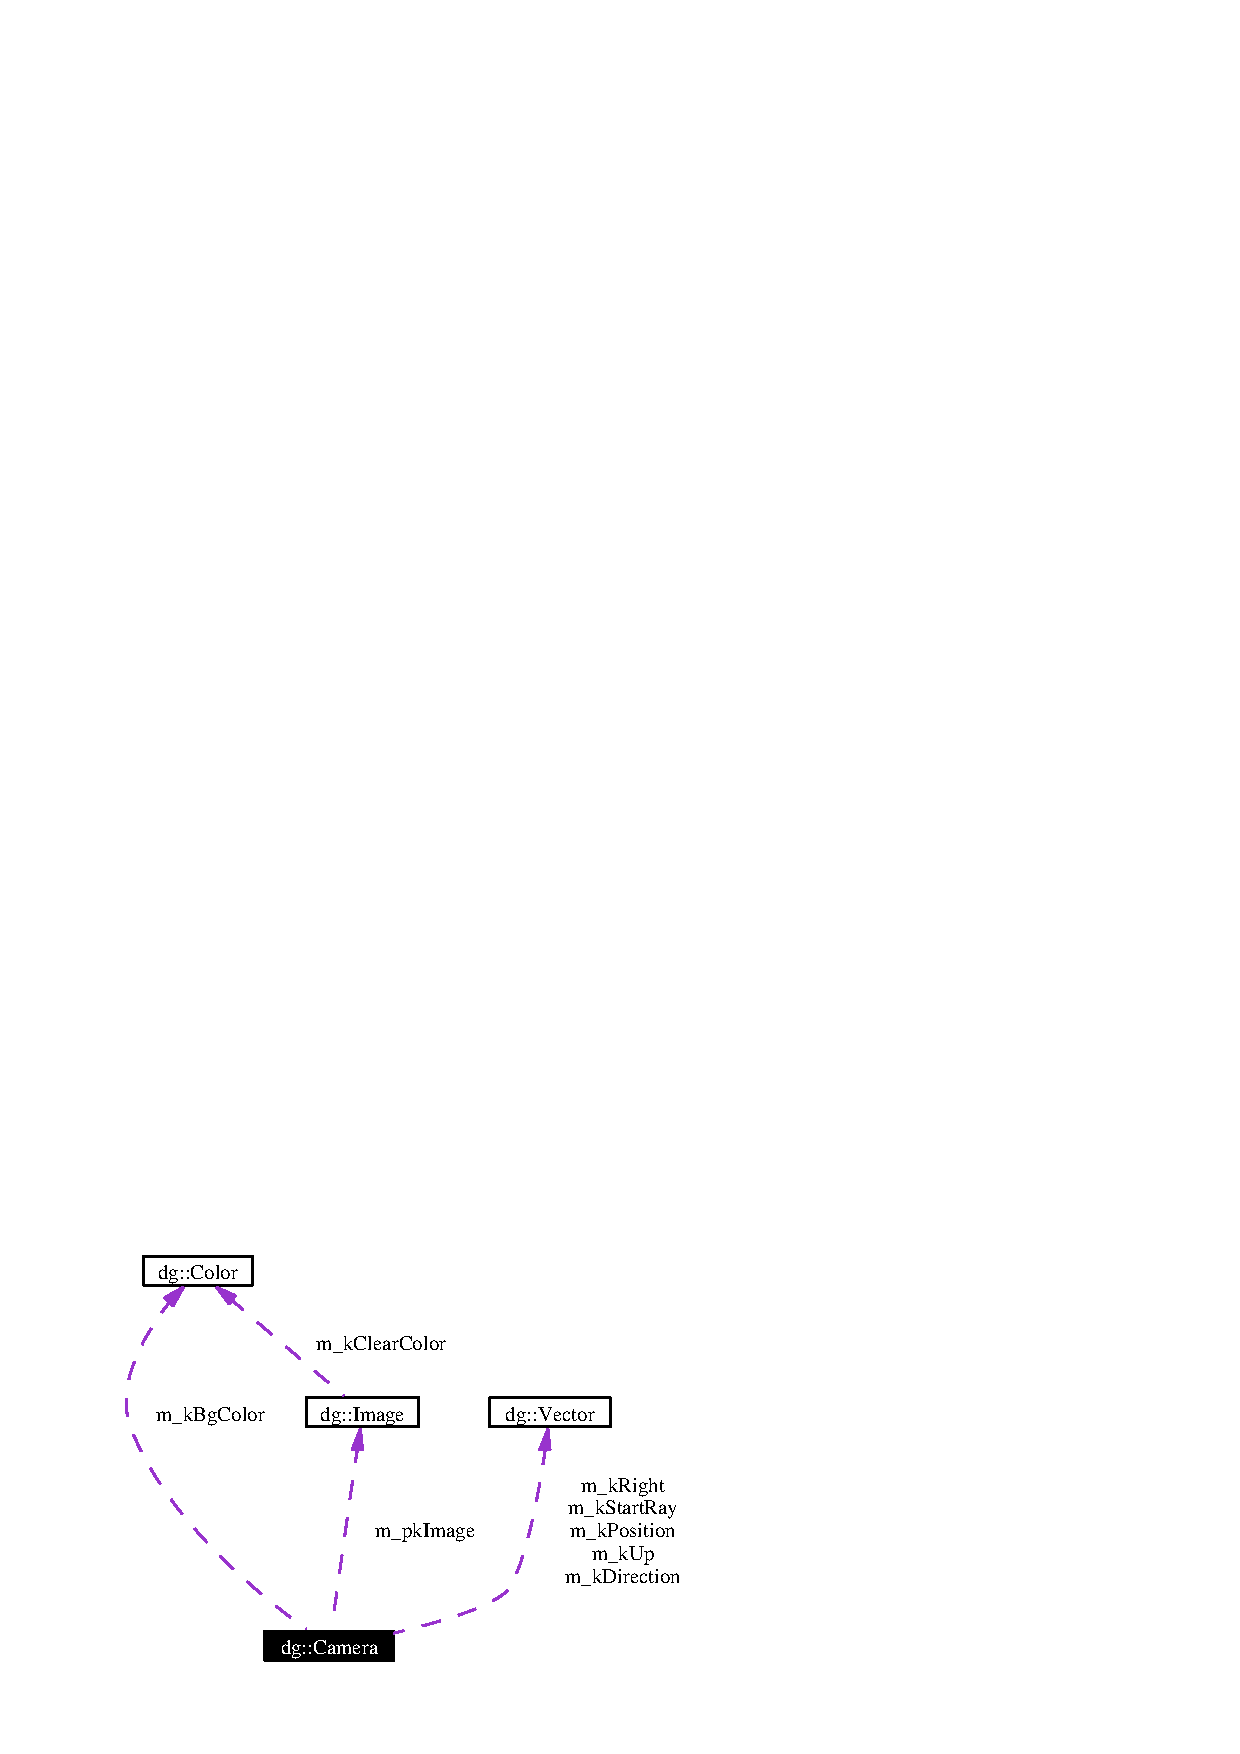
\includegraphics[width=172pt]{classdg_1_1Camera__coll__graph}
\end{center}
\end{figure}
\subsection*{Public Methods}
\begin{CompactItemize}
\item 
{\bf Camera} (const {\bf Vector} \&rk\-Pos={\bf Vector}(0.0f, 0.0f, 0.0f), const {\bf Vector} \&rk\-Dir={\bf Vector}(0.0f, 0.0f, 1.0f), const {\bf Vector} \&rk\-Up={\bf Vector}(0.0f, 1.0f, 0.0f), const {\bf Vector} \&rk\-Right={\bf Vector}(1.0f, 0.0f, 0.0f), {\bf Real} f\-Near=0.1f, {\bf Real} f\-Far=10.0f, {\bf Real} f\-Half\-Width=0.5f, {\bf Real} f\-Half\-Height=0.5f, {\bf Image} $\ast$pk\-Image=NULL)
\item 
{\bf $\sim$Camera} ()
\item 
void {\bf setup} ()
\item 
{\bf Vector} {\bf get\-Position} () const
\item 
void {\bf set\-Position} (const {\bf Vector} \&rk\-Position)
\item 
{\bf Vector} {\bf get\-Direction} () const
\item 
void {\bf set\-Direction} (const {\bf Vector} \&rk\-Direction)
\item 
{\bf Vector} {\bf get\-Up} () const
\item 
void {\bf set\-Up} (const {\bf Vector} \&rk\-Up)
\item 
{\bf Vector} {\bf get\-Right} () const
\item 
void {\bf set\-Right} (const {\bf Vector} \&rk\-Right)
\item 
void {\bf set\-Near} ({\bf Real} f\-Near)
\item 
{\bf Real} {\bf get\-Near} () const
\item 
void {\bf set\-Far} ({\bf Real} f\-Far)
\item 
{\bf Real} {\bf get\-Far} () const
\item 
void {\bf set\-Half\-Width} ({\bf Real} f\-Half\-Width)
\item 
{\bf Real} {\bf get\-Half\-Width} () const
\item 
void {\bf set\-Horizontal\-Fov} ({\bf Real} f\-Horiz\-Fov)
\item 
{\bf Real} {\bf get\-Horizontal\-Fov} () const
\item 
void {\bf set\-Half\-Height} ({\bf Real} f\-Half\-Height)
\item 
{\bf Real} {\bf get\-Half\-Height} () const
\item 
void {\bf set\-Vertical\-Fov} ({\bf Real} f\-Vert\-Fov)
\item 
{\bf Real} {\bf get\-Vertical\-Fov} () const
\item 
void {\bf set\-Background} (const {\bf Color} \&rk\-Color)
\item 
{\bf Color} {\bf get\-Background} () const
\item 
{\bf Vector} {\bf get\-Ray\-Dir} ({\bf UInt} ui\-X, {\bf UInt} ui\-Y) const
\item 
{\bf Vector} {\bf get\-Start\-Ray\-Dir} () const
\item 
void {\bf set\-Image} ({\bf Image} $\ast$pk\-Image)
\item 
const {\bf Image} $\ast$ {\bf get\-Image} () const
\item 
{\bf Image} $\ast$ {\bf get\-Image} ()
\item 
{\bf UInt} {\bf get\-Image\-Width} () const
\item 
{\bf UInt} {\bf get\-Image\-Height} () const
\item 
{\bf UInt} {\bf get\-Image\-Channels} () const
\item 
{\bf Real} {\bf get\-Pixel\-Width} () const
\item 
{\bf Real} {\bf get\-Pixel\-Height} () const
\end{CompactItemize}


\subsection{Constructor \& Destructor Documentation}
\index{dg::Camera@{dg::Camera}!Camera@{Camera}}
\index{Camera@{Camera}!dg::Camera@{dg::Camera}}
\subsubsection{\setlength{\rightskip}{0pt plus 5cm}Camera::Camera (const {\bf Vector} \& {\em rk\-Pos} = {\bf Vector}(0.0f, 0.0f, 0.0f), const {\bf Vector} \& {\em rk\-Dir} = {\bf Vector}(0.0f, 0.0f, 1.0f), const {\bf Vector} \& {\em rk\-Up} = {\bf Vector}(0.0f, 1.0f, 0.0f), const {\bf Vector} \& {\em rk\-Right} = {\bf Vector}(1.0f, 0.0f, 0.0f), {\bf Real} {\em f\-Near} = 0.1f, {\bf Real} {\em f\-Far} = 10.0f, {\bf Real} {\em f\-Half\-Width} = 0.5f, {\bf Real} {\em f\-Half\-Height} = 0.5f, {\bf Image} $\ast$ {\em pk\-Image} = NULL)}\label{classdg_1_1Camera_a0}




Definition at line 7 of file Camera.cpp.

References dg::Real.\index{dg::Camera@{dg::Camera}!~Camera@{$\sim$Camera}}
\index{~Camera@{$\sim$Camera}!dg::Camera@{dg::Camera}}
\subsubsection{\setlength{\rightskip}{0pt plus 5cm}Camera::$\sim$Camera ()}\label{classdg_1_1Camera_a1}




Definition at line 25 of file Camera.cpp.

\subsection{Member Function Documentation}
\index{dg::Camera@{dg::Camera}!getBackground@{getBackground}}
\index{getBackground@{getBackground}!dg::Camera@{dg::Camera}}
\subsubsection{\setlength{\rightskip}{0pt plus 5cm}{\bf Color} dg::Camera::get\-Background ()\hspace{0.3cm}{\tt  [inline]}}\label{classdg_1_1Camera_a24}




Definition at line 257 of file Camera.h.\index{dg::Camera@{dg::Camera}!getDirection@{getDirection}}
\index{getDirection@{getDirection}!dg::Camera@{dg::Camera}}
\subsubsection{\setlength{\rightskip}{0pt plus 5cm}{\bf Vector} dg::Camera::get\-Direction ()\hspace{0.3cm}{\tt  [inline]}}\label{classdg_1_1Camera_a5}




Definition at line 143 of file Camera.h.

Referenced by dg::Visualizer::draw\-Polygons(), dg::Visualizer::on\-Startup(), dg::Ray\-Tracer::render(), dg::Hypertexture::render(), dg::Visualizer::setup\-Camera(), and dg::Visualizer::setup\-Ray\-Tracer().\index{dg::Camera@{dg::Camera}!getFar@{getFar}}
\index{getFar@{getFar}!dg::Camera@{dg::Camera}}
\subsubsection{\setlength{\rightskip}{0pt plus 5cm}{\bf Real} dg::Camera::get\-Far ()\hspace{0.3cm}{\tt  [inline]}}\label{classdg_1_1Camera_a14}




Definition at line 183 of file Camera.h.

Referenced by dg::Ray\-Tracer::render(), and dg::Hypertexture::render().\index{dg::Camera@{dg::Camera}!getHalfHeight@{getHalfHeight}}
\index{getHalfHeight@{getHalfHeight}!dg::Camera@{dg::Camera}}
\subsubsection{\setlength{\rightskip}{0pt plus 5cm}{\bf Real} dg::Camera::get\-Half\-Height ()\hspace{0.3cm}{\tt  [inline]}}\label{classdg_1_1Camera_a20}




Definition at line 203 of file Camera.h.

Referenced by dg::Ray\-Tracer::render(), and dg::Hypertexture::render().\index{dg::Camera@{dg::Camera}!getHalfWidth@{getHalfWidth}}
\index{getHalfWidth@{getHalfWidth}!dg::Camera@{dg::Camera}}
\subsubsection{\setlength{\rightskip}{0pt plus 5cm}{\bf Real} dg::Camera::get\-Half\-Width ()\hspace{0.3cm}{\tt  [inline]}}\label{classdg_1_1Camera_a16}




Definition at line 193 of file Camera.h.

Referenced by dg::Ray\-Tracer::render(), and dg::Hypertexture::render().\index{dg::Camera@{dg::Camera}!getHorizontalFov@{getHorizontalFov}}
\index{getHorizontalFov@{getHorizontalFov}!dg::Camera@{dg::Camera}}
\subsubsection{\setlength{\rightskip}{0pt plus 5cm}{\bf Real} Camera::get\-Horizontal\-Fov ()\hspace{0.3cm}{\tt  [inline]}}\label{classdg_1_1Camera_a18}




Definition at line 35 of file Camera.cpp.

References dg::Arc\-Tangent(), dg::Degrees(), and dg::Real.\index{dg::Camera@{dg::Camera}!getImage@{getImage}}
\index{getImage@{getImage}!dg::Camera@{dg::Camera}}
\subsubsection{\setlength{\rightskip}{0pt plus 5cm}{\bf Image} $\ast$ dg::Camera::get\-Image ()\hspace{0.3cm}{\tt  [inline]}}\label{classdg_1_1Camera_a29}




Definition at line 247 of file Camera.h.\index{dg::Camera@{dg::Camera}!getImage@{getImage}}
\index{getImage@{getImage}!dg::Camera@{dg::Camera}}
\subsubsection{\setlength{\rightskip}{0pt plus 5cm}const {\bf Image} $\ast$ dg::Camera::get\-Image ()\hspace{0.3cm}{\tt  [inline]}}\label{classdg_1_1Camera_a28}




Definition at line 242 of file Camera.h.

Referenced by dg::Ray\-Tracer::render(), and dg::Hypertexture::render().\index{dg::Camera@{dg::Camera}!getImageChannels@{getImageChannels}}
\index{getImageChannels@{getImageChannels}!dg::Camera@{dg::Camera}}
\subsubsection{\setlength{\rightskip}{0pt plus 5cm}{\bf UInt} dg::Camera::get\-Image\-Channels ()\hspace{0.3cm}{\tt  [inline]}}\label{classdg_1_1Camera_a32}




Definition at line 229 of file Camera.h.\index{dg::Camera@{dg::Camera}!getImageHeight@{getImageHeight}}
\index{getImageHeight@{getImageHeight}!dg::Camera@{dg::Camera}}
\subsubsection{\setlength{\rightskip}{0pt plus 5cm}{\bf UInt} dg::Camera::get\-Image\-Height ()\hspace{0.3cm}{\tt  [inline]}}\label{classdg_1_1Camera_a31}




Definition at line 221 of file Camera.h.\index{dg::Camera@{dg::Camera}!getImageWidth@{getImageWidth}}
\index{getImageWidth@{getImageWidth}!dg::Camera@{dg::Camera}}
\subsubsection{\setlength{\rightskip}{0pt plus 5cm}{\bf UInt} dg::Camera::get\-Image\-Width ()\hspace{0.3cm}{\tt  [inline]}}\label{classdg_1_1Camera_a30}




Definition at line 213 of file Camera.h.\index{dg::Camera@{dg::Camera}!getNear@{getNear}}
\index{getNear@{getNear}!dg::Camera@{dg::Camera}}
\subsubsection{\setlength{\rightskip}{0pt plus 5cm}{\bf Real} dg::Camera::get\-Near ()\hspace{0.3cm}{\tt  [inline]}}\label{classdg_1_1Camera_a12}




Definition at line 173 of file Camera.h.

Referenced by dg::Ray\-Tracer::render(), and dg::Hypertexture::render().\index{dg::Camera@{dg::Camera}!getPixelHeight@{getPixelHeight}}
\index{getPixelHeight@{getPixelHeight}!dg::Camera@{dg::Camera}}
\subsubsection{\setlength{\rightskip}{0pt plus 5cm}{\bf Real} dg::Camera::get\-Pixel\-Height ()\hspace{0.3cm}{\tt  [inline]}}\label{classdg_1_1Camera_a34}




Definition at line 272 of file Camera.h.\index{dg::Camera@{dg::Camera}!getPixelWidth@{getPixelWidth}}
\index{getPixelWidth@{getPixelWidth}!dg::Camera@{dg::Camera}}
\subsubsection{\setlength{\rightskip}{0pt plus 5cm}{\bf Real} dg::Camera::get\-Pixel\-Width ()\hspace{0.3cm}{\tt  [inline]}}\label{classdg_1_1Camera_a33}




Definition at line 267 of file Camera.h.\index{dg::Camera@{dg::Camera}!getPosition@{getPosition}}
\index{getPosition@{getPosition}!dg::Camera@{dg::Camera}}
\subsubsection{\setlength{\rightskip}{0pt plus 5cm}{\bf Vector} dg::Camera::get\-Position ()\hspace{0.3cm}{\tt  [inline]}}\label{classdg_1_1Camera_a3}




Definition at line 133 of file Camera.h.

Referenced by dg::Visualizer::draw\-Polygons(), dg::Ray\-Tracer::render(), and dg::Visualizer::setup\-Camera().\index{dg::Camera@{dg::Camera}!getRayDir@{getRayDir}}
\index{getRayDir@{getRayDir}!dg::Camera@{dg::Camera}}
\subsubsection{\setlength{\rightskip}{0pt plus 5cm}{\bf Vector} Camera::get\-Ray\-Dir ({\bf UInt} {\em ui\-X}, {\bf UInt} {\em ui\-Y}) const}\label{classdg_1_1Camera_a25}




Definition at line 50 of file Camera.cpp.

References dg::Vector::normalize(), dg::UInt, dg::Vector::x(), dg::Vector::y(), and dg::Vector::z().\index{dg::Camera@{dg::Camera}!getRight@{getRight}}
\index{getRight@{getRight}!dg::Camera@{dg::Camera}}
\subsubsection{\setlength{\rightskip}{0pt plus 5cm}{\bf Vector} dg::Camera::get\-Right ()\hspace{0.3cm}{\tt  [inline]}}\label{classdg_1_1Camera_a9}




Definition at line 163 of file Camera.h.

Referenced by dg::Ray\-Tracer::render(), and dg::Hypertexture::render().\index{dg::Camera@{dg::Camera}!getStartRayDir@{getStartRayDir}}
\index{getStartRayDir@{getStartRayDir}!dg::Camera@{dg::Camera}}
\subsubsection{\setlength{\rightskip}{0pt plus 5cm}{\bf Vector} dg::Camera::get\-Start\-Ray\-Dir ()\hspace{0.3cm}{\tt  [inline]}}\label{classdg_1_1Camera_a26}




Definition at line 262 of file Camera.h.\index{dg::Camera@{dg::Camera}!getUp@{getUp}}
\index{getUp@{getUp}!dg::Camera@{dg::Camera}}
\subsubsection{\setlength{\rightskip}{0pt plus 5cm}{\bf Vector} dg::Camera::get\-Up ()\hspace{0.3cm}{\tt  [inline]}}\label{classdg_1_1Camera_a7}




Definition at line 153 of file Camera.h.

Referenced by dg::Visualizer::draw\-Polygons(), dg::Ray\-Tracer::render(), dg::Hypertexture::render(), and dg::Visualizer::setup\-Camera().\index{dg::Camera@{dg::Camera}!getVerticalFov@{getVerticalFov}}
\index{getVerticalFov@{getVerticalFov}!dg::Camera@{dg::Camera}}
\subsubsection{\setlength{\rightskip}{0pt plus 5cm}{\bf Real} Camera::get\-Vertical\-Fov ()\hspace{0.3cm}{\tt  [inline]}}\label{classdg_1_1Camera_a22}




Definition at line 45 of file Camera.cpp.

References dg::Arc\-Tangent(), dg::Degrees(), and dg::Real.\index{dg::Camera@{dg::Camera}!setBackground@{setBackground}}
\index{setBackground@{setBackground}!dg::Camera@{dg::Camera}}
\subsubsection{\setlength{\rightskip}{0pt plus 5cm}void dg::Camera::set\-Background (const {\bf Color} \& {\em rk\-Color})\hspace{0.3cm}{\tt  [inline]}}\label{classdg_1_1Camera_a23}




Definition at line 252 of file Camera.h.\index{dg::Camera@{dg::Camera}!setDirection@{setDirection}}
\index{setDirection@{setDirection}!dg::Camera@{dg::Camera}}
\subsubsection{\setlength{\rightskip}{0pt plus 5cm}void dg::Camera::set\-Direction (const {\bf Vector} \& {\em rk\-Direction})\hspace{0.3cm}{\tt  [inline]}}\label{classdg_1_1Camera_a6}




Definition at line 148 of file Camera.h.

Referenced by dg::Visualizer::setup\-Camera().\index{dg::Camera@{dg::Camera}!setFar@{setFar}}
\index{setFar@{setFar}!dg::Camera@{dg::Camera}}
\subsubsection{\setlength{\rightskip}{0pt plus 5cm}void dg::Camera::set\-Far ({\bf Real} {\em f\-Far})\hspace{0.3cm}{\tt  [inline]}}\label{classdg_1_1Camera_a13}




Definition at line 188 of file Camera.h.

Referenced by dg::Visualizer::setup\-Camera().\index{dg::Camera@{dg::Camera}!setHalfHeight@{setHalfHeight}}
\index{setHalfHeight@{setHalfHeight}!dg::Camera@{dg::Camera}}
\subsubsection{\setlength{\rightskip}{0pt plus 5cm}void dg::Camera::set\-Half\-Height ({\bf Real} {\em f\-Half\-Height})\hspace{0.3cm}{\tt  [inline]}}\label{classdg_1_1Camera_a19}




Definition at line 208 of file Camera.h.

Referenced by dg::Visualizer::setup\-Camera().\index{dg::Camera@{dg::Camera}!setHalfWidth@{setHalfWidth}}
\index{setHalfWidth@{setHalfWidth}!dg::Camera@{dg::Camera}}
\subsubsection{\setlength{\rightskip}{0pt plus 5cm}void dg::Camera::set\-Half\-Width ({\bf Real} {\em f\-Half\-Width})\hspace{0.3cm}{\tt  [inline]}}\label{classdg_1_1Camera_a15}




Definition at line 198 of file Camera.h.

Referenced by dg::Visualizer::setup\-Camera().\index{dg::Camera@{dg::Camera}!setHorizontalFov@{setHorizontalFov}}
\index{setHorizontalFov@{setHorizontalFov}!dg::Camera@{dg::Camera}}
\subsubsection{\setlength{\rightskip}{0pt plus 5cm}void Camera::set\-Horizontal\-Fov ({\bf Real} {\em f\-Horiz\-Fov})\hspace{0.3cm}{\tt  [inline]}}\label{classdg_1_1Camera_a17}




Definition at line 30 of file Camera.cpp.

References dg::Radians(), dg::Real, and dg::Tangent().\index{dg::Camera@{dg::Camera}!setImage@{setImage}}
\index{setImage@{setImage}!dg::Camera@{dg::Camera}}
\subsubsection{\setlength{\rightskip}{0pt plus 5cm}void dg::Camera::set\-Image ({\bf Image} $\ast$ {\em pk\-Image})\hspace{0.3cm}{\tt  [inline]}}\label{classdg_1_1Camera_a27}




Definition at line 237 of file Camera.h.

Referenced by dg::Visualizer::setup\-Hypertexture(), and dg::Visualizer::setup\-Ray\-Tracer().\index{dg::Camera@{dg::Camera}!setNear@{setNear}}
\index{setNear@{setNear}!dg::Camera@{dg::Camera}}
\subsubsection{\setlength{\rightskip}{0pt plus 5cm}void dg::Camera::set\-Near ({\bf Real} {\em f\-Near})\hspace{0.3cm}{\tt  [inline]}}\label{classdg_1_1Camera_a11}




Definition at line 178 of file Camera.h.

Referenced by dg::Visualizer::setup\-Camera().\index{dg::Camera@{dg::Camera}!setPosition@{setPosition}}
\index{setPosition@{setPosition}!dg::Camera@{dg::Camera}}
\subsubsection{\setlength{\rightskip}{0pt plus 5cm}void dg::Camera::set\-Position (const {\bf Vector} \& {\em rk\-Position})\hspace{0.3cm}{\tt  [inline]}}\label{classdg_1_1Camera_a4}




Definition at line 138 of file Camera.h.

Referenced by dg::Visualizer::setup\-Camera().\index{dg::Camera@{dg::Camera}!setRight@{setRight}}
\index{setRight@{setRight}!dg::Camera@{dg::Camera}}
\subsubsection{\setlength{\rightskip}{0pt plus 5cm}void dg::Camera::set\-Right (const {\bf Vector} \& {\em rk\-Right})\hspace{0.3cm}{\tt  [inline]}}\label{classdg_1_1Camera_a10}




Definition at line 168 of file Camera.h.

Referenced by dg::Visualizer::setup\-Camera().\index{dg::Camera@{dg::Camera}!setUp@{setUp}}
\index{setUp@{setUp}!dg::Camera@{dg::Camera}}
\subsubsection{\setlength{\rightskip}{0pt plus 5cm}void dg::Camera::set\-Up (const {\bf Vector} \& {\em rk\-Up})\hspace{0.3cm}{\tt  [inline]}}\label{classdg_1_1Camera_a8}




Definition at line 158 of file Camera.h.

Referenced by dg::Visualizer::setup\-Camera().\index{dg::Camera@{dg::Camera}!setup@{setup}}
\index{setup@{setup}!dg::Camera@{dg::Camera}}
\subsubsection{\setlength{\rightskip}{0pt plus 5cm}void Camera::setup ()}\label{classdg_1_1Camera_a2}




Definition at line 96 of file Camera.cpp.

References dg::Image::height(), dg::Real, dg::Image::width(), dg::Vector::x(), dg::Vector::y(), and dg::Vector::z().\index{dg::Camera@{dg::Camera}!setVerticalFov@{setVerticalFov}}
\index{setVerticalFov@{setVerticalFov}!dg::Camera@{dg::Camera}}
\subsubsection{\setlength{\rightskip}{0pt plus 5cm}void Camera::set\-Vertical\-Fov ({\bf Real} {\em f\-Vert\-Fov})\hspace{0.3cm}{\tt  [inline]}}\label{classdg_1_1Camera_a21}




Definition at line 40 of file Camera.cpp.

References dg::Radians(), dg::Real, and dg::Tangent().

The documentation for this class was generated from the following files:\begin{CompactItemize}
\item 
{\bf Camera.h}\item 
{\bf Camera.cpp}\end{CompactItemize}

\section{dg::Color Class Reference}
\label{classdg_1_1Color}\index{dg::Color@{dg::Color}}
{\tt \#include $<$Color.h$>$}

\subsection*{Public Methods}
\begin{CompactItemize}
\item 
{\bf Color} ()
\item 
{\bf Color} ({\bf Real} d\-R, {\bf Real} d\-G, {\bf Real} d\-B, {\bf Real} d\-A=1.0)
\item 
{\bf Color} (const Color \&rk\-Color)
\item 
{\bf Real} {\bf r} () const
\item 
{\bf Real} {\bf g} () const
\item 
{\bf Real} {\bf b} () const
\item 
{\bf Real} {\bf a} () const
\item 
{\bf Real} \& {\bf r} ()
\item 
{\bf Real} \& {\bf g} ()
\item 
{\bf Real} \& {\bf b} ()
\item 
{\bf Real} \& {\bf a} ()
\item 
{\bf Real} {\bf operator()} ({\bf UInt} ui\-C) const
\item 
{\bf Real} {\bf operator[$\,$]} ({\bf UInt} ui\-C) const
\item 
{\bf Real} \& {\bf operator()} ({\bf UInt} ui\-C)
\item 
{\bf Real} \& {\bf operator[$\,$]} ({\bf UInt} ui\-C)
\item 
{\bf Real} {\bf get\-Component} ({\bf UInt} ui\-C) const
\item 
const Color \& {\bf value} ()
\item 
{\bf Real} $\ast$ {\bf values} ()
\item 
void {\bf set} (const Color \&v)
\item 
void {\bf set} ({\bf Real} r, {\bf Real} g, {\bf Real} b, {\bf Real} a=1.0)
\item 
void {\bf set\-Red} ({\bf Real} r)
\item 
void {\bf set\-Green} ({\bf Real} g)
\item 
void {\bf set\-Blue} ({\bf Real} b)
\item 
void {\bf set\-Alpha} ({\bf Real} a)
\item 
void {\bf set\-Component} ({\bf Real} n, {\bf UInt} c)
\item 
void {\bf operator=} (const Color \&rk\-Color)
\item 
{\bf Bool} {\bf operator==} (const Color \&rk\-Color) const
\item 
{\bf Bool} {\bf operator!=} (const Color \&rk\-Color) const
\item 
Color {\bf operator+} (const Color \&rk\-Color) const
\item 
void {\bf operator++} (void)
\item 
void {\bf operator+=} (const Color \&rk\-Color)
\item 
Color {\bf operator-} () const
\item 
Color {\bf operator-} (const Color \&rk\-Color) const
\item 
void {\bf operator--} (void)
\item 
void {\bf operator-=} (const Color \&rk\-Color)
\item 
Color {\bf operator $\ast$} (const Color \&rk\-Color) const
\item 
void {\bf operator $\ast$=} (const Color \&rk\-Color)
\item 
Color {\bf operator $\ast$} (const {\bf Int} scalar) const
\item 
void {\bf operator $\ast$=} (const {\bf Int} scalar)
\item 
Color {\bf operator $\ast$} (const {\bf Real} scalar) const
\item 
void {\bf operator $\ast$=} (const {\bf Real} scalar)
\item 
void {\bf zero} ()
\item 
void {\bf negate} ()
\end{CompactItemize}
\subsection*{Static Public Attributes}
\begin{CompactItemize}
\item 
const Color {\bf BLACK} = Color(0.0f, 0.0f, 0.0f)
\item 
const Color {\bf GRAY} = Color(0.5f, 0.5f, 0.5f)
\item 
const Color {\bf WHITE} = Color(1.0f, 1.0f, 1.0f)
\end{CompactItemize}


\subsection{Constructor \& Destructor Documentation}
\index{dg::Color@{dg::Color}!Color@{Color}}
\index{Color@{Color}!dg::Color@{dg::Color}}
\subsubsection{\setlength{\rightskip}{0pt plus 5cm}Color::Color ()}\label{classdg_1_1Color_a0}




Definition at line 20 of file Color.cpp.\index{dg::Color@{dg::Color}!Color@{Color}}
\index{Color@{Color}!dg::Color@{dg::Color}}
\subsubsection{\setlength{\rightskip}{0pt plus 5cm}Color::Color ({\bf Real} {\em d\-R}, {\bf Real} {\em d\-G}, {\bf Real} {\em d\-B}, {\bf Real} {\em d\-A} = 1.0)}\label{classdg_1_1Color_a1}




Definition at line 28 of file Color.cpp.

References dg::Real.\index{dg::Color@{dg::Color}!Color@{Color}}
\index{Color@{Color}!dg::Color@{dg::Color}}
\subsubsection{\setlength{\rightskip}{0pt plus 5cm}Color::Color (const Color \& {\em rk\-Color})}\label{classdg_1_1Color_a2}




Definition at line 36 of file Color.cpp.

References m\_\-ad\-C.

\subsection{Member Function Documentation}
\index{dg::Color@{dg::Color}!a@{a}}
\index{a@{a}!dg::Color@{dg::Color}}
\subsubsection{\setlength{\rightskip}{0pt plus 5cm}{\bf Real} \& dg::Color::a ()\hspace{0.3cm}{\tt  [inline]}}\label{classdg_1_1Color_a10}




Definition at line 134 of file Color.h.\index{dg::Color@{dg::Color}!a@{a}}
\index{a@{a}!dg::Color@{dg::Color}}
\subsubsection{\setlength{\rightskip}{0pt plus 5cm}{\bf Real} dg::Color::a ()\hspace{0.3cm}{\tt  [inline]}}\label{classdg_1_1Color_a6}




Definition at line 114 of file Color.h.

Referenced by dg::Window::draw\-String(), and dg::Visualizer::draw\-Text().\index{dg::Color@{dg::Color}!b@{b}}
\index{b@{b}!dg::Color@{dg::Color}}
\subsubsection{\setlength{\rightskip}{0pt plus 5cm}{\bf Real} \& dg::Color::b ()\hspace{0.3cm}{\tt  [inline]}}\label{classdg_1_1Color_a9}




Definition at line 129 of file Color.h.\index{dg::Color@{dg::Color}!b@{b}}
\index{b@{b}!dg::Color@{dg::Color}}
\subsubsection{\setlength{\rightskip}{0pt plus 5cm}{\bf Real} dg::Color::b ()\hspace{0.3cm}{\tt  [inline]}}\label{classdg_1_1Color_a5}




Definition at line 109 of file Color.h.

Referenced by dg::Clamp(), dg::Window::draw\-String(), dg::Visualizer::draw\-Text(), and dg::operator $\ast$().\index{dg::Color@{dg::Color}!g@{g}}
\index{g@{g}!dg::Color@{dg::Color}}
\subsubsection{\setlength{\rightskip}{0pt plus 5cm}{\bf Real} \& dg::Color::g ()\hspace{0.3cm}{\tt  [inline]}}\label{classdg_1_1Color_a8}




Definition at line 124 of file Color.h.\index{dg::Color@{dg::Color}!g@{g}}
\index{g@{g}!dg::Color@{dg::Color}}
\subsubsection{\setlength{\rightskip}{0pt plus 5cm}{\bf Real} dg::Color::g ()\hspace{0.3cm}{\tt  [inline]}}\label{classdg_1_1Color_a4}




Definition at line 104 of file Color.h.

Referenced by dg::Clamp(), dg::Window::draw\-String(), dg::Visualizer::draw\-Text(), and dg::operator $\ast$().\index{dg::Color@{dg::Color}!getComponent@{getComponent}}
\index{getComponent@{getComponent}!dg::Color@{dg::Color}}
\subsubsection{\setlength{\rightskip}{0pt plus 5cm}{\bf Real} dg::Color::get\-Component ({\bf UInt} {\em ui\-C}) const\hspace{0.3cm}{\tt  [inline]}}\label{classdg_1_1Color_a15}




Definition at line 171 of file Color.h.\index{dg::Color@{dg::Color}!negate@{negate}}
\index{negate@{negate}!dg::Color@{dg::Color}}
\subsubsection{\setlength{\rightskip}{0pt plus 5cm}void dg::Color::negate ()\hspace{0.3cm}{\tt  [inline]}}\label{classdg_1_1Color_a42}




Definition at line 239 of file Color.h.\index{dg::Color@{dg::Color}!operator *@{operator $\ast$}}
\index{operator *@{operator $\ast$}!dg::Color@{dg::Color}}
\subsubsection{\setlength{\rightskip}{0pt plus 5cm}Color Color::operator $\ast$ (const {\bf Real} {\em scalar}) const}\label{classdg_1_1Color_a39}




Definition at line 142 of file Color.cpp.

References dg::Real.\index{dg::Color@{dg::Color}!operator *@{operator $\ast$}}
\index{operator *@{operator $\ast$}!dg::Color@{dg::Color}}
\subsubsection{\setlength{\rightskip}{0pt plus 5cm}Color Color::operator $\ast$ (const {\bf Int} {\em scalar}) const}\label{classdg_1_1Color_a37}




Definition at line 124 of file Color.cpp.

References dg::Int.\index{dg::Color@{dg::Color}!operator *@{operator $\ast$}}
\index{operator *@{operator $\ast$}!dg::Color@{dg::Color}}
\subsubsection{\setlength{\rightskip}{0pt plus 5cm}Color Color::operator $\ast$ (const Color \& {\em rk\-Color}) const}\label{classdg_1_1Color_a35}




Definition at line 106 of file Color.cpp.

References m\_\-ad\-C.\index{dg::Color@{dg::Color}!operator *=@{operator $\ast$=}}
\index{operator *=@{operator $\ast$=}!dg::Color@{dg::Color}}
\subsubsection{\setlength{\rightskip}{0pt plus 5cm}void Color::operator $\ast$= (const {\bf Real} {\em scalar})}\label{classdg_1_1Color_a40}




Definition at line 152 of file Color.cpp.

References dg::Real.\index{dg::Color@{dg::Color}!operator *=@{operator $\ast$=}}
\index{operator *=@{operator $\ast$=}!dg::Color@{dg::Color}}
\subsubsection{\setlength{\rightskip}{0pt plus 5cm}void Color::operator $\ast$= (const {\bf Int} {\em scalar})}\label{classdg_1_1Color_a38}




Definition at line 134 of file Color.cpp.

References dg::Int.\index{dg::Color@{dg::Color}!operator *=@{operator $\ast$=}}
\index{operator *=@{operator $\ast$=}!dg::Color@{dg::Color}}
\subsubsection{\setlength{\rightskip}{0pt plus 5cm}void Color::operator $\ast$= (const Color \& {\em rk\-Color})}\label{classdg_1_1Color_a36}




Definition at line 116 of file Color.cpp.

References m\_\-ad\-C.\index{dg::Color@{dg::Color}!operator"!=@{operator"!=}}
\index{operator"!=@{operator"!=}!dg::Color@{dg::Color}}
\subsubsection{\setlength{\rightskip}{0pt plus 5cm}{\bf Bool} Color::operator!= (const Color \& {\em rk\-Color}) const}\label{classdg_1_1Color_a27}




Definition at line 178 of file Color.cpp.

References dg::Bool.\index{dg::Color@{dg::Color}!operator()@{operator()}}
\index{operator()@{operator()}!dg::Color@{dg::Color}}
\subsubsection{\setlength{\rightskip}{0pt plus 5cm}{\bf Real} \& dg::Color::operator() ({\bf UInt} {\em ui\-C})\hspace{0.3cm}{\tt  [inline]}}\label{classdg_1_1Color_a13}




Definition at line 163 of file Color.h.\index{dg::Color@{dg::Color}!operator()@{operator()}}
\index{operator()@{operator()}!dg::Color@{dg::Color}}
\subsubsection{\setlength{\rightskip}{0pt plus 5cm}{\bf Real} dg::Color::operator() ({\bf UInt} {\em ui\-C}) const\hspace{0.3cm}{\tt  [inline]}}\label{classdg_1_1Color_a11}




Definition at line 147 of file Color.h.\index{dg::Color@{dg::Color}!operator+@{operator+}}
\index{operator+@{operator+}!dg::Color@{dg::Color}}
\subsubsection{\setlength{\rightskip}{0pt plus 5cm}Color Color::operator+ (const Color \& {\em rk\-Color}) const}\label{classdg_1_1Color_a28}




Definition at line 44 of file Color.cpp.

References m\_\-ad\-C.\index{dg::Color@{dg::Color}!operator++@{operator++}}
\index{operator++@{operator++}!dg::Color@{dg::Color}}
\subsubsection{\setlength{\rightskip}{0pt plus 5cm}void Color::operator++ (void)}\label{classdg_1_1Color_a29}




Definition at line 54 of file Color.cpp.\index{dg::Color@{dg::Color}!operator+=@{operator+=}}
\index{operator+=@{operator+=}!dg::Color@{dg::Color}}
\subsubsection{\setlength{\rightskip}{0pt plus 5cm}void Color::operator+= (const Color \& {\em rk\-Color})}\label{classdg_1_1Color_a30}




Definition at line 62 of file Color.cpp.

References m\_\-ad\-C.\index{dg::Color@{dg::Color}!operator-@{operator-}}
\index{operator-@{operator-}!dg::Color@{dg::Color}}
\subsubsection{\setlength{\rightskip}{0pt plus 5cm}Color Color::operator- (const Color \& {\em rk\-Color}) const}\label{classdg_1_1Color_a32}




Definition at line 80 of file Color.cpp.

References m\_\-ad\-C.\index{dg::Color@{dg::Color}!operator-@{operator-}}
\index{operator-@{operator-}!dg::Color@{dg::Color}}
\subsubsection{\setlength{\rightskip}{0pt plus 5cm}Color Color::operator- ()}\label{classdg_1_1Color_a31}




Definition at line 70 of file Color.cpp.\index{dg::Color@{dg::Color}!operator--@{operator--}}
\index{operator--@{operator--}!dg::Color@{dg::Color}}
\subsubsection{\setlength{\rightskip}{0pt plus 5cm}void Color::operator-- (void)}\label{classdg_1_1Color_a33}




Definition at line 90 of file Color.cpp.\index{dg::Color@{dg::Color}!operator-=@{operator-=}}
\index{operator-=@{operator-=}!dg::Color@{dg::Color}}
\subsubsection{\setlength{\rightskip}{0pt plus 5cm}void Color::operator-= (const Color \& {\em rk\-Color})}\label{classdg_1_1Color_a34}




Definition at line 98 of file Color.cpp.

References m\_\-ad\-C.\index{dg::Color@{dg::Color}!operator=@{operator=}}
\index{operator=@{operator=}!dg::Color@{dg::Color}}
\subsubsection{\setlength{\rightskip}{0pt plus 5cm}void Color::operator= (const Color \& {\em rk\-Color})}\label{classdg_1_1Color_a25}




Definition at line 160 of file Color.cpp.

References m\_\-ad\-C.\index{dg::Color@{dg::Color}!operator==@{operator==}}
\index{operator==@{operator==}!dg::Color@{dg::Color}}
\subsubsection{\setlength{\rightskip}{0pt plus 5cm}{\bf Bool} Color::operator== (const Color \& {\em rk\-Color}) const}\label{classdg_1_1Color_a26}




Definition at line 168 of file Color.cpp.

References dg::Bool, and m\_\-ad\-C.\index{dg::Color@{dg::Color}!operator[]@{operator[]}}
\index{operator[]@{operator[]}!dg::Color@{dg::Color}}
\subsubsection{\setlength{\rightskip}{0pt plus 5cm}{\bf Real} \& dg::Color::operator[$\,$] ({\bf UInt} {\em ui\-C})\hspace{0.3cm}{\tt  [inline]}}\label{classdg_1_1Color_a14}




Definition at line 155 of file Color.h.\index{dg::Color@{dg::Color}!operator[]@{operator[]}}
\index{operator[]@{operator[]}!dg::Color@{dg::Color}}
\subsubsection{\setlength{\rightskip}{0pt plus 5cm}{\bf Real} dg::Color::operator[$\,$] ({\bf UInt} {\em ui\-C}) const\hspace{0.3cm}{\tt  [inline]}}\label{classdg_1_1Color_a12}




Definition at line 139 of file Color.h.\index{dg::Color@{dg::Color}!r@{r}}
\index{r@{r}!dg::Color@{dg::Color}}
\subsubsection{\setlength{\rightskip}{0pt plus 5cm}{\bf Real} \& dg::Color::r ()\hspace{0.3cm}{\tt  [inline]}}\label{classdg_1_1Color_a7}




Definition at line 119 of file Color.h.\index{dg::Color@{dg::Color}!r@{r}}
\index{r@{r}!dg::Color@{dg::Color}}
\subsubsection{\setlength{\rightskip}{0pt plus 5cm}{\bf Real} dg::Color::r ()\hspace{0.3cm}{\tt  [inline]}}\label{classdg_1_1Color_a3}




Definition at line 99 of file Color.h.

Referenced by dg::Clamp(), dg::Window::draw\-String(), dg::Visualizer::draw\-Text(), and dg::operator $\ast$().\index{dg::Color@{dg::Color}!set@{set}}
\index{set@{set}!dg::Color@{dg::Color}}
\subsubsection{\setlength{\rightskip}{0pt plus 5cm}void dg::Color::set ({\bf Real} {\em r}, {\bf Real} {\em g}, {\bf Real} {\em b}, {\bf Real} {\em a} = 1.0)\hspace{0.3cm}{\tt  [inline]}}\label{classdg_1_1Color_a19}




Definition at line 197 of file Color.h.\index{dg::Color@{dg::Color}!set@{set}}
\index{set@{set}!dg::Color@{dg::Color}}
\subsubsection{\setlength{\rightskip}{0pt plus 5cm}void dg::Color::set (const Color \& {\em v})\hspace{0.3cm}{\tt  [inline]}}\label{classdg_1_1Color_a18}




Definition at line 189 of file Color.h.\index{dg::Color@{dg::Color}!setAlpha@{setAlpha}}
\index{setAlpha@{setAlpha}!dg::Color@{dg::Color}}
\subsubsection{\setlength{\rightskip}{0pt plus 5cm}void dg::Color::set\-Alpha ({\bf Real} {\em a})\hspace{0.3cm}{\tt  [inline]}}\label{classdg_1_1Color_a23}




Definition at line 220 of file Color.h.\index{dg::Color@{dg::Color}!setBlue@{setBlue}}
\index{setBlue@{setBlue}!dg::Color@{dg::Color}}
\subsubsection{\setlength{\rightskip}{0pt plus 5cm}void dg::Color::set\-Blue ({\bf Real} {\em b})\hspace{0.3cm}{\tt  [inline]}}\label{classdg_1_1Color_a22}




Definition at line 215 of file Color.h.\index{dg::Color@{dg::Color}!setComponent@{setComponent}}
\index{setComponent@{setComponent}!dg::Color@{dg::Color}}
\subsubsection{\setlength{\rightskip}{0pt plus 5cm}void dg::Color::set\-Component ({\bf Real} {\em n}, {\bf UInt} {\em c})\hspace{0.3cm}{\tt  [inline]}}\label{classdg_1_1Color_a24}




Definition at line 225 of file Color.h.\index{dg::Color@{dg::Color}!setGreen@{setGreen}}
\index{setGreen@{setGreen}!dg::Color@{dg::Color}}
\subsubsection{\setlength{\rightskip}{0pt plus 5cm}void dg::Color::set\-Green ({\bf Real} {\em g})\hspace{0.3cm}{\tt  [inline]}}\label{classdg_1_1Color_a21}




Definition at line 210 of file Color.h.\index{dg::Color@{dg::Color}!setRed@{setRed}}
\index{setRed@{setRed}!dg::Color@{dg::Color}}
\subsubsection{\setlength{\rightskip}{0pt plus 5cm}void dg::Color::set\-Red ({\bf Real} {\em r})\hspace{0.3cm}{\tt  [inline]}}\label{classdg_1_1Color_a20}




Definition at line 205 of file Color.h.\index{dg::Color@{dg::Color}!value@{value}}
\index{value@{value}!dg::Color@{dg::Color}}
\subsubsection{\setlength{\rightskip}{0pt plus 5cm}const Color \& dg::Color::value ()\hspace{0.3cm}{\tt  [inline]}}\label{classdg_1_1Color_a16}




Definition at line 179 of file Color.h.\index{dg::Color@{dg::Color}!values@{values}}
\index{values@{values}!dg::Color@{dg::Color}}
\subsubsection{\setlength{\rightskip}{0pt plus 5cm}{\bf Real} $\ast$ dg::Color::values ()\hspace{0.3cm}{\tt  [inline]}}\label{classdg_1_1Color_a17}




Definition at line 184 of file Color.h.\index{dg::Color@{dg::Color}!zero@{zero}}
\index{zero@{zero}!dg::Color@{dg::Color}}
\subsubsection{\setlength{\rightskip}{0pt plus 5cm}void dg::Color::zero ()\hspace{0.3cm}{\tt  [inline]}}\label{classdg_1_1Color_a41}




Definition at line 231 of file Color.h.

\subsection{Member Data Documentation}
\index{dg::Color@{dg::Color}!BLACK@{BLACK}}
\index{BLACK@{BLACK}!dg::Color@{dg::Color}}
\subsubsection{\setlength{\rightskip}{0pt plus 5cm}const Color Color::BLACK = Color(0.0f, 0.0f, 0.0f)\hspace{0.3cm}{\tt  [static]}}\label{classdg_1_1Color_p0}




Definition at line 201 of file Color.cpp.\index{dg::Color@{dg::Color}!GRAY@{GRAY}}
\index{GRAY@{GRAY}!dg::Color@{dg::Color}}
\subsubsection{\setlength{\rightskip}{0pt plus 5cm}const Color Color::GRAY = Color(0.5f, 0.5f, 0.5f)\hspace{0.3cm}{\tt  [static]}}\label{classdg_1_1Color_p1}




Definition at line 202 of file Color.cpp.\index{dg::Color@{dg::Color}!WHITE@{WHITE}}
\index{WHITE@{WHITE}!dg::Color@{dg::Color}}
\subsubsection{\setlength{\rightskip}{0pt plus 5cm}const Color Color::WHITE = Color(1.0f, 1.0f, 1.0f)\hspace{0.3cm}{\tt  [static]}}\label{classdg_1_1Color_p2}




Definition at line 203 of file Color.cpp.

The documentation for this class was generated from the following files:\begin{CompactItemize}
\item 
{\bf Color.h}\item 
{\bf Color.cpp}\end{CompactItemize}

\section{dg::Hypertexture Class Reference}
\label{classdg_1_1Hypertexture}\index{dg::Hypertexture@{dg::Hypertexture}}
{\tt \#include $<$Hypertexture.h$>$}

Collaboration diagram for dg::Hypertexture:\begin{figure}[H]
\begin{center}
\leavevmode
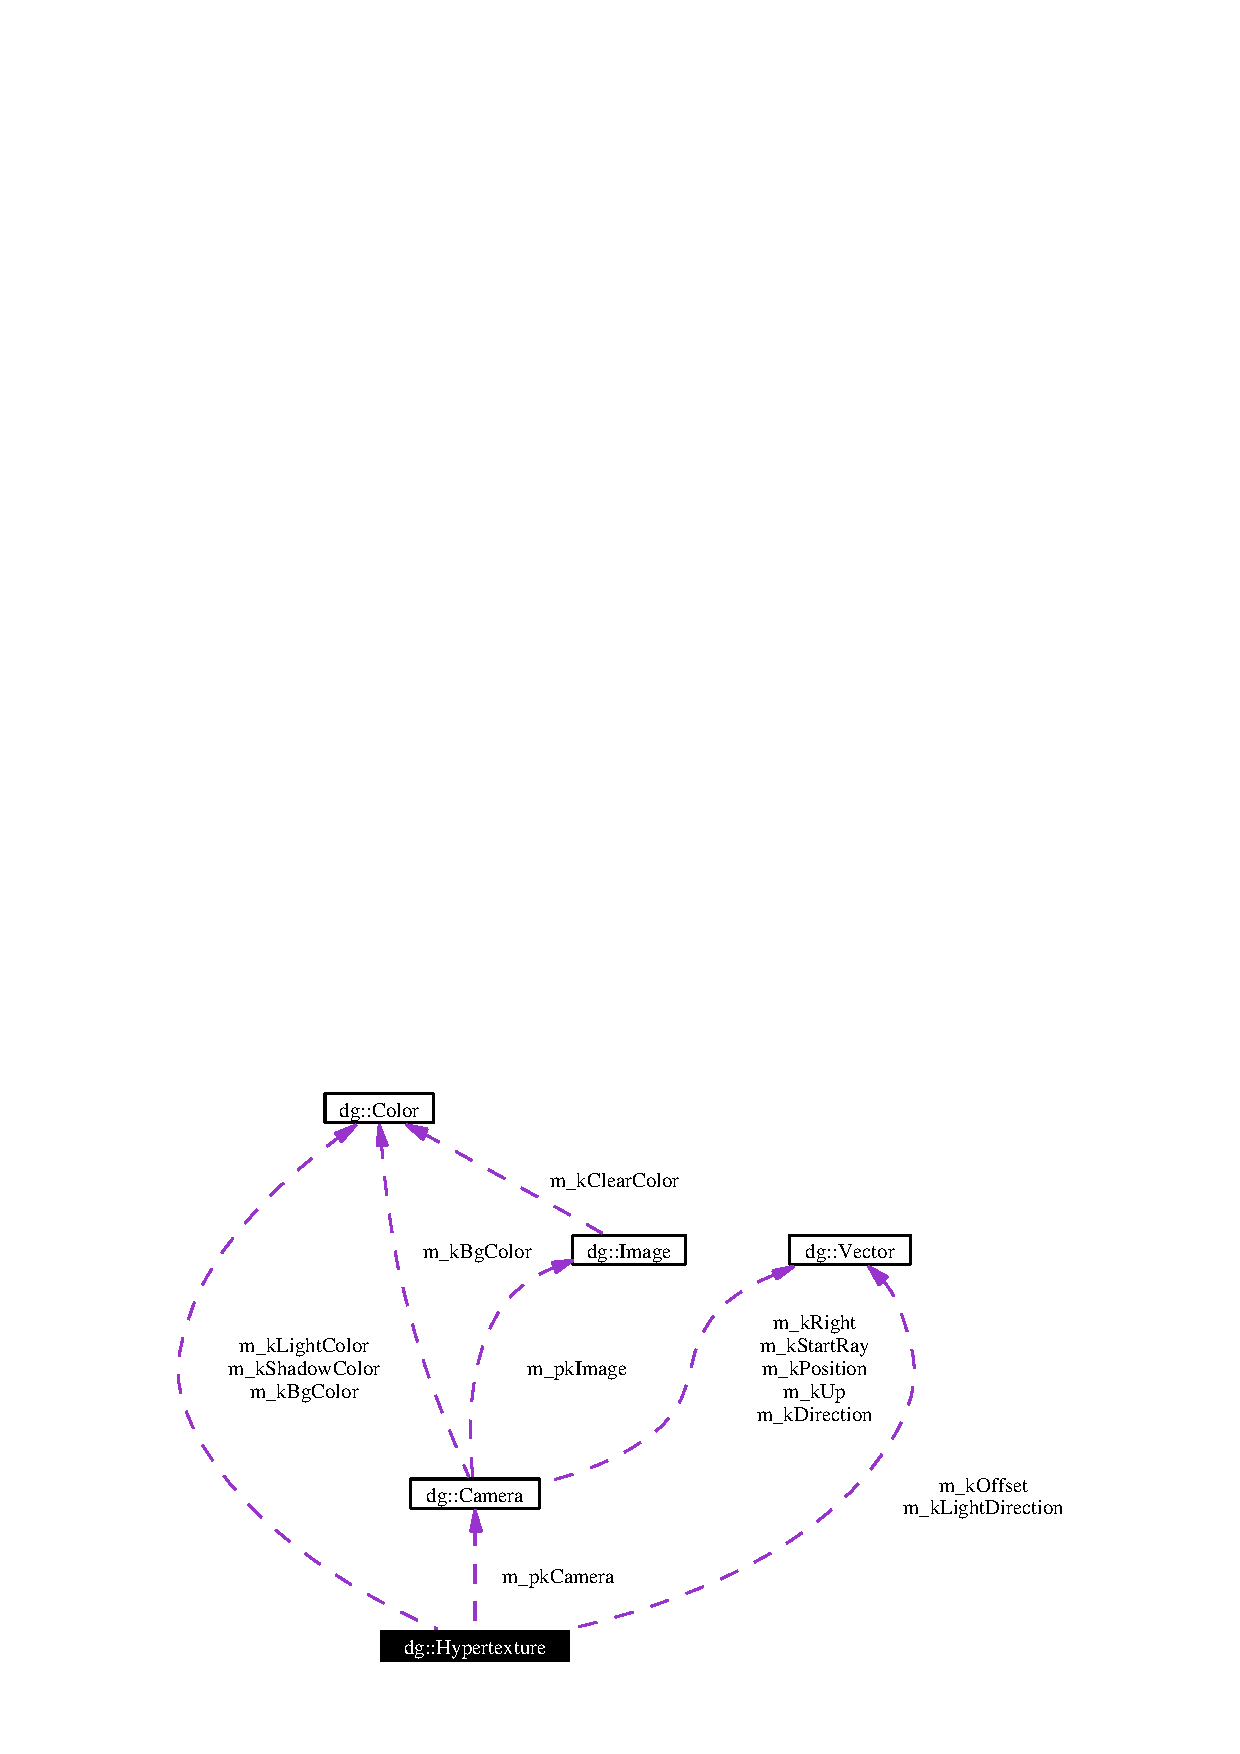
\includegraphics[width=274pt]{classdg_1_1Hypertexture__coll__graph}
\end{center}
\end{figure}
\subsection*{Public Types}
\begin{CompactItemize}
\item 
typedef {\bf Real}($\ast$ {\bf Density\-Fn} )({\bf Real} f\-X, {\bf Real} f\-Y, {\bf Real} f\-Z)
\item 
typedef {\bf Real}($\ast$ {\bf Filtered\-Density\-Fn} )({\bf Real} f\-X, {\bf Real} f\-Y, {\bf Real} f\-Z, {\bf Real} f\-DT)
\item 
typedef {\bf Color}($\ast$ {\bf Color\-Fn} )({\bf Real} f\-X, {\bf Real} f\-Y, {\bf Real} f\-Z)
\item 
typedef {\bf Color}($\ast$ {\bf Filtered\-Color\-Fn} )({\bf Real} f\-X, {\bf Real} f\-Y, {\bf Real} f\-Z, {\bf Real} f\-DT)
\item 
typedef {\bf Color}($\ast$ {\bf Shade\-Fn} )(const {\bf Vector} \&rk\-Surface\-Normal, const {\bf Vector} \&rk\-View\-Dir, const {\bf Vector} \&rk\-Light\-Dir, const {\bf Color} \&rk\-Light\-Color, const {\bf Color} \&rk\-Base\-Color, {\bf Real} f\-Ambient, {\bf Real} f\-Diffuse, {\bf Real} f\-Specular, {\bf Real} f\-Roughness)
\end{CompactItemize}
\subsection*{Public Methods}
\begin{CompactItemize}
\item 
{\bf Hypertexture::Hypertexture} ({\bf Density\-Fn} pv\-Density\-Fn=NULL, {\bf Color\-Fn} pv\-Color\-Fn=NULL, {\bf Shade\-Fn} pv\-Shade\-Fn=NULL, {\bf Camera} $\ast$pk\-Camera=NULL)
\item 
{\bf $\sim$Hypertexture} ()
\item 
void {\bf set\-Density\-Function} ({\bf Density\-Fn} pv\-Density\-Fn)
\item 
void {\bf set\-Color\-Function} ({\bf Color\-Fn} pv\-Color\-Fn)
\item 
void {\bf set\-Shading\-Function} ({\bf Shade\-Fn} pv\-Shade\-Fn)
\item 
void {\bf set\-Filtered\-Density\-Function} ({\bf Filtered\-Density\-Fn} pv\-Density\-Fn)
\item 
void {\bf set\-Filtered\-Color\-Function} ({\bf Filtered\-Color\-Fn} pv\-Color\-Fn)
\item 
void {\bf set\-Camera} ({\bf Camera} $\ast$pk\-Camera)
\item 
const {\bf Camera} $\ast$ {\bf get\-Camera} () const
\item 
{\bf Vector} {\bf get\-Light\-Direction} () const
\item 
void {\bf set\-Light\-Direction} (const {\bf Vector} \&rk\-Light)
\item 
{\bf Color} {\bf get\-Light\-Color} () const
\item 
void {\bf set\-Light\-Color} (const {\bf Color} \&rk\-Light)
\item 
void {\bf set\-Scale} ({\bf Real} f\-Scale)
\item 
{\bf Real} {\bf get\-Scale} ()
\item 
{\bf Real} {\bf get\-Ambient} () const
\item 
void {\bf set\-Ambient} ({\bf Real} f\-Ambient)
\item 
{\bf Real} {\bf get\-Diffuse} () const
\item 
void {\bf set\-Diffuse} ({\bf Real} f\-Diffuse)
\item 
{\bf Real} {\bf get\-Specular} () const
\item 
void {\bf set\-Specular} ({\bf Real} f\-Specular)
\item 
{\bf Real} {\bf get\-Roughness} () const
\item 
void {\bf set\-Roughness} ({\bf Real} f\-Roughness)
\item 
void {\bf set\-Ray\-Epsilon} ({\bf Real} f\-Epsilon)
\item 
{\bf Real} {\bf get\-Ray\-Epsilon} () const
\item 
{\bf Real} {\bf get\-Density\-Scale} () const
\item 
void {\bf set\-Density\-Scale} ({\bf Real} f\-Density\-Scale)
\item 
{\bf Real} {\bf get\-Density\-Threshold} () const
\item 
void {\bf set\-Density\-Threshold} ({\bf Real} f\-Density\-Threshold)
\item 
{\bf Real} {\bf get\-Opacity\-Threshold} () const
\item 
void {\bf set\-Opacity\-Threshold} ({\bf Real} f\-Opacity\-Threshold)
\item 
{\bf Real} {\bf get\-Shadow\-Far\-Clip} () const
\item 
void {\bf set\-Shadow\-Far\-Clip} ({\bf Real} f\-Shadow\-Far\-Clip)
\item 
{\bf Real} {\bf get\-Shadow\-Depth\-Threshold} () const
\item 
void {\bf set\-Shadow\-Depth\-Threshold} ({\bf Real} f\-Shadow\-Depth\-Threshold)
\item 
{\bf Real} {\bf get\-Shadow\-Step\-Scale} () const
\item 
void {\bf set\-Shadow\-Step\-Scale} ({\bf Real} f\-Shadow\-Step\-Scale)
\item 
{\bf Real} {\bf get\-Step\-Size} () const
\item 
void {\bf set\-Step\-Size} ({\bf Real} f\-Step\-Size)
\item 
void {\bf set\-Max\-Samples} ({\bf UInt} ui\-Max)
\item 
{\bf UInt} {\bf get\-Max\-Samples} () const
\item 
{\bf UInt} {\bf get\-Ray\-Hits} () const
\item 
{\bf UInt} {\bf get\-Samples} () const
\item 
void {\bf set\-Background} (const {\bf Color} \&rk\-Color)
\item 
{\bf Color} {\bf get\-Background} () const
\item 
void {\bf set\-Keep\-In\-View} (bool b\-Keep\-In\-View)
\item 
bool {\bf get\-Keep\-In\-View} ()
\item 
void {\bf set\-Fade\-Out} (bool b\-Fade\-Out)
\item 
bool {\bf get\-Fade\-Out} ()
\item 
void {\bf render} ()
\item 
void {\bf render} ({\bf UInt} ui\-Start\-Line, {\bf UInt} ui\-End\-Line)
\end{CompactItemize}


\subsection{Member Typedef Documentation}
\index{dg::Hypertexture@{dg::Hypertexture}!ColorFn@{ColorFn}}
\index{ColorFn@{ColorFn}!dg::Hypertexture@{dg::Hypertexture}}
\subsubsection{\setlength{\rightskip}{0pt plus 5cm}typedef {\bf Color}($\ast$ dg::Hypertexture::Color\-Fn)({\bf Real} f\-X, {\bf Real} f\-Y, {\bf Real} f\-Z)}\label{classdg_1_1Hypertexture_s2}




Definition at line 22 of file Hypertexture.h.\index{dg::Hypertexture@{dg::Hypertexture}!DensityFn@{DensityFn}}
\index{DensityFn@{DensityFn}!dg::Hypertexture@{dg::Hypertexture}}
\subsubsection{\setlength{\rightskip}{0pt plus 5cm}typedef {\bf Real}($\ast$ dg::Hypertexture::Density\-Fn)({\bf Real} f\-X, {\bf Real} f\-Y, {\bf Real} f\-Z)}\label{classdg_1_1Hypertexture_s0}




Definition at line 19 of file Hypertexture.h.\index{dg::Hypertexture@{dg::Hypertexture}!FilteredColorFn@{FilteredColorFn}}
\index{FilteredColorFn@{FilteredColorFn}!dg::Hypertexture@{dg::Hypertexture}}
\subsubsection{\setlength{\rightskip}{0pt plus 5cm}typedef {\bf Color}($\ast$ dg::Hypertexture::Filtered\-Color\-Fn)({\bf Real} f\-X, {\bf Real} f\-Y, {\bf Real} f\-Z, {\bf Real} f\-DT)}\label{classdg_1_1Hypertexture_s3}




Definition at line 23 of file Hypertexture.h.\index{dg::Hypertexture@{dg::Hypertexture}!FilteredDensityFn@{FilteredDensityFn}}
\index{FilteredDensityFn@{FilteredDensityFn}!dg::Hypertexture@{dg::Hypertexture}}
\subsubsection{\setlength{\rightskip}{0pt plus 5cm}typedef {\bf Real}($\ast$ dg::Hypertexture::Filtered\-Density\-Fn)({\bf Real} f\-X, {\bf Real} f\-Y, {\bf Real} f\-Z, {\bf Real} f\-DT)}\label{classdg_1_1Hypertexture_s1}




Definition at line 20 of file Hypertexture.h.\index{dg::Hypertexture@{dg::Hypertexture}!ShadeFn@{ShadeFn}}
\index{ShadeFn@{ShadeFn}!dg::Hypertexture@{dg::Hypertexture}}
\subsubsection{\setlength{\rightskip}{0pt plus 5cm}typedef {\bf Color}($\ast$ dg::Hypertexture::Shade\-Fn)(const {\bf Vector}\& rk\-Surface\-Normal, const {\bf Vector}\& rk\-View\-Dir, const {\bf Vector}\& rk\-Light\-Dir, const {\bf Color}\& rk\-Light\-Color, const {\bf Color}\& rk\-Base\-Color, {\bf Real} f\-Ambient, {\bf Real} f\-Diffuse, {\bf Real} f\-Specular, {\bf Real} f\-Roughness)}\label{classdg_1_1Hypertexture_s4}




Definition at line 25 of file Hypertexture.h.

\subsection{Constructor \& Destructor Documentation}
\index{dg::Hypertexture@{dg::Hypertexture}!~Hypertexture@{$\sim$Hypertexture}}
\index{~Hypertexture@{$\sim$Hypertexture}!dg::Hypertexture@{dg::Hypertexture}}
\subsubsection{\setlength{\rightskip}{0pt plus 5cm}Hypertexture::$\sim$Hypertexture ()}\label{classdg_1_1Hypertexture_a1}




Definition at line 63 of file Hypertexture.cpp.

\subsection{Member Function Documentation}
\index{dg::Hypertexture@{dg::Hypertexture}!getAmbient@{getAmbient}}
\index{getAmbient@{getAmbient}!dg::Hypertexture@{dg::Hypertexture}}
\subsubsection{\setlength{\rightskip}{0pt plus 5cm}{\bf Real} dg::Hypertexture::get\-Ambient ()\hspace{0.3cm}{\tt  [inline]}}\label{classdg_1_1Hypertexture_a15}




Definition at line 403 of file Hypertexture.h.\index{dg::Hypertexture@{dg::Hypertexture}!getBackground@{getBackground}}
\index{getBackground@{getBackground}!dg::Hypertexture@{dg::Hypertexture}}
\subsubsection{\setlength{\rightskip}{0pt plus 5cm}{\bf Color} dg::Hypertexture::get\-Background ()\hspace{0.3cm}{\tt  [inline]}}\label{classdg_1_1Hypertexture_a44}




Definition at line 299 of file Hypertexture.h.\index{dg::Hypertexture@{dg::Hypertexture}!getCamera@{getCamera}}
\index{getCamera@{getCamera}!dg::Hypertexture@{dg::Hypertexture}}
\subsubsection{\setlength{\rightskip}{0pt plus 5cm}const {\bf Camera} $\ast$ dg::Hypertexture::get\-Camera ()\hspace{0.3cm}{\tt  [inline]}}\label{classdg_1_1Hypertexture_a8}




Definition at line 309 of file Hypertexture.h.\index{dg::Hypertexture@{dg::Hypertexture}!getDensityScale@{getDensityScale}}
\index{getDensityScale@{getDensityScale}!dg::Hypertexture@{dg::Hypertexture}}
\subsubsection{\setlength{\rightskip}{0pt plus 5cm}{\bf Real} dg::Hypertexture::get\-Density\-Scale ()\hspace{0.3cm}{\tt  [inline]}}\label{classdg_1_1Hypertexture_a25}




Definition at line 254 of file Hypertexture.h.\index{dg::Hypertexture@{dg::Hypertexture}!getDensityThreshold@{getDensityThreshold}}
\index{getDensityThreshold@{getDensityThreshold}!dg::Hypertexture@{dg::Hypertexture}}
\subsubsection{\setlength{\rightskip}{0pt plus 5cm}{\bf Real} dg::Hypertexture::get\-Density\-Threshold ()\hspace{0.3cm}{\tt  [inline]}}\label{classdg_1_1Hypertexture_a27}




Definition at line 264 of file Hypertexture.h.\index{dg::Hypertexture@{dg::Hypertexture}!getDiffuse@{getDiffuse}}
\index{getDiffuse@{getDiffuse}!dg::Hypertexture@{dg::Hypertexture}}
\subsubsection{\setlength{\rightskip}{0pt plus 5cm}{\bf Real} dg::Hypertexture::get\-Diffuse ()\hspace{0.3cm}{\tt  [inline]}}\label{classdg_1_1Hypertexture_a17}




Definition at line 413 of file Hypertexture.h.\index{dg::Hypertexture@{dg::Hypertexture}!getFadeOut@{getFadeOut}}
\index{getFadeOut@{getFadeOut}!dg::Hypertexture@{dg::Hypertexture}}
\subsubsection{\setlength{\rightskip}{0pt plus 5cm}bool dg::Hypertexture::get\-Fade\-Out ()\hspace{0.3cm}{\tt  [inline]}}\label{classdg_1_1Hypertexture_a48}




Definition at line 458 of file Hypertexture.h.\index{dg::Hypertexture@{dg::Hypertexture}!getKeepInView@{getKeepInView}}
\index{getKeepInView@{getKeepInView}!dg::Hypertexture@{dg::Hypertexture}}
\subsubsection{\setlength{\rightskip}{0pt plus 5cm}bool dg::Hypertexture::get\-Keep\-In\-View ()\hspace{0.3cm}{\tt  [inline]}}\label{classdg_1_1Hypertexture_a46}




Definition at line 448 of file Hypertexture.h.\index{dg::Hypertexture@{dg::Hypertexture}!getLightColor@{getLightColor}}
\index{getLightColor@{getLightColor}!dg::Hypertexture@{dg::Hypertexture}}
\subsubsection{\setlength{\rightskip}{0pt plus 5cm}{\bf Color} dg::Hypertexture::get\-Light\-Color ()\hspace{0.3cm}{\tt  [inline]}}\label{classdg_1_1Hypertexture_a11}




Definition at line 244 of file Hypertexture.h.\index{dg::Hypertexture@{dg::Hypertexture}!getLightDirection@{getLightDirection}}
\index{getLightDirection@{getLightDirection}!dg::Hypertexture@{dg::Hypertexture}}
\subsubsection{\setlength{\rightskip}{0pt plus 5cm}{\bf Vector} dg::Hypertexture::get\-Light\-Direction ()\hspace{0.3cm}{\tt  [inline]}}\label{classdg_1_1Hypertexture_a9}




Definition at line 234 of file Hypertexture.h.\index{dg::Hypertexture@{dg::Hypertexture}!getMaxSamples@{getMaxSamples}}
\index{getMaxSamples@{getMaxSamples}!dg::Hypertexture@{dg::Hypertexture}}
\subsubsection{\setlength{\rightskip}{0pt plus 5cm}{\bf UInt} dg::Hypertexture::get\-Max\-Samples ()\hspace{0.3cm}{\tt  [inline]}}\label{classdg_1_1Hypertexture_a40}




Definition at line 343 of file Hypertexture.h.\index{dg::Hypertexture@{dg::Hypertexture}!getOpacityThreshold@{getOpacityThreshold}}
\index{getOpacityThreshold@{getOpacityThreshold}!dg::Hypertexture@{dg::Hypertexture}}
\subsubsection{\setlength{\rightskip}{0pt plus 5cm}{\bf Real} dg::Hypertexture::get\-Opacity\-Threshold ()\hspace{0.3cm}{\tt  [inline]}}\label{classdg_1_1Hypertexture_a29}




Definition at line 274 of file Hypertexture.h.\index{dg::Hypertexture@{dg::Hypertexture}!getRayEpsilon@{getRayEpsilon}}
\index{getRayEpsilon@{getRayEpsilon}!dg::Hypertexture@{dg::Hypertexture}}
\subsubsection{\setlength{\rightskip}{0pt plus 5cm}{\bf Real} dg::Hypertexture::get\-Ray\-Epsilon ()\hspace{0.3cm}{\tt  [inline]}}\label{classdg_1_1Hypertexture_a24}




Definition at line 353 of file Hypertexture.h.\index{dg::Hypertexture@{dg::Hypertexture}!getRayHits@{getRayHits}}
\index{getRayHits@{getRayHits}!dg::Hypertexture@{dg::Hypertexture}}
\subsubsection{\setlength{\rightskip}{0pt plus 5cm}{\bf UInt} dg::Hypertexture::get\-Ray\-Hits ()\hspace{0.3cm}{\tt  [inline]}}\label{classdg_1_1Hypertexture_a41}




Definition at line 284 of file Hypertexture.h.

Referenced by dg::Visualizer::draw\-Text().\index{dg::Hypertexture@{dg::Hypertexture}!getRoughness@{getRoughness}}
\index{getRoughness@{getRoughness}!dg::Hypertexture@{dg::Hypertexture}}
\subsubsection{\setlength{\rightskip}{0pt plus 5cm}{\bf Real} dg::Hypertexture::get\-Roughness ()\hspace{0.3cm}{\tt  [inline]}}\label{classdg_1_1Hypertexture_a21}




Definition at line 433 of file Hypertexture.h.\index{dg::Hypertexture@{dg::Hypertexture}!getSamples@{getSamples}}
\index{getSamples@{getSamples}!dg::Hypertexture@{dg::Hypertexture}}
\subsubsection{\setlength{\rightskip}{0pt plus 5cm}{\bf UInt} dg::Hypertexture::get\-Samples ()\hspace{0.3cm}{\tt  [inline]}}\label{classdg_1_1Hypertexture_a42}




Definition at line 289 of file Hypertexture.h.

Referenced by dg::Visualizer::draw\-Text().\index{dg::Hypertexture@{dg::Hypertexture}!getScale@{getScale}}
\index{getScale@{getScale}!dg::Hypertexture@{dg::Hypertexture}}
\subsubsection{\setlength{\rightskip}{0pt plus 5cm}{\bf Real} dg::Hypertexture::get\-Scale ()\hspace{0.3cm}{\tt  [inline]}}\label{classdg_1_1Hypertexture_a14}




Definition at line 468 of file Hypertexture.h.\index{dg::Hypertexture@{dg::Hypertexture}!getShadowDepthThreshold@{getShadowDepthThreshold}}
\index{getShadowDepthThreshold@{getShadowDepthThreshold}!dg::Hypertexture@{dg::Hypertexture}}
\subsubsection{\setlength{\rightskip}{0pt plus 5cm}{\bf Real} dg::Hypertexture::get\-Shadow\-Depth\-Threshold ()\hspace{0.3cm}{\tt  [inline]}}\label{classdg_1_1Hypertexture_a33}




Definition at line 373 of file Hypertexture.h.\index{dg::Hypertexture@{dg::Hypertexture}!getShadowFarClip@{getShadowFarClip}}
\index{getShadowFarClip@{getShadowFarClip}!dg::Hypertexture@{dg::Hypertexture}}
\subsubsection{\setlength{\rightskip}{0pt plus 5cm}{\bf Real} dg::Hypertexture::get\-Shadow\-Far\-Clip ()\hspace{0.3cm}{\tt  [inline]}}\label{classdg_1_1Hypertexture_a31}




Definition at line 363 of file Hypertexture.h.\index{dg::Hypertexture@{dg::Hypertexture}!getShadowStepScale@{getShadowStepScale}}
\index{getShadowStepScale@{getShadowStepScale}!dg::Hypertexture@{dg::Hypertexture}}
\subsubsection{\setlength{\rightskip}{0pt plus 5cm}{\bf Real} dg::Hypertexture::get\-Shadow\-Step\-Scale ()\hspace{0.3cm}{\tt  [inline]}}\label{classdg_1_1Hypertexture_a35}




Definition at line 383 of file Hypertexture.h.\index{dg::Hypertexture@{dg::Hypertexture}!getSpecular@{getSpecular}}
\index{getSpecular@{getSpecular}!dg::Hypertexture@{dg::Hypertexture}}
\subsubsection{\setlength{\rightskip}{0pt plus 5cm}{\bf Real} dg::Hypertexture::get\-Specular ()\hspace{0.3cm}{\tt  [inline]}}\label{classdg_1_1Hypertexture_a19}




Definition at line 423 of file Hypertexture.h.\index{dg::Hypertexture@{dg::Hypertexture}!getStepSize@{getStepSize}}
\index{getStepSize@{getStepSize}!dg::Hypertexture@{dg::Hypertexture}}
\subsubsection{\setlength{\rightskip}{0pt plus 5cm}{\bf Real} dg::Hypertexture::get\-Step\-Size ()\hspace{0.3cm}{\tt  [inline]}}\label{classdg_1_1Hypertexture_a37}




Definition at line 393 of file Hypertexture.h.

Referenced by dg::Visualizer::draw\-Text().\index{dg::Hypertexture@{dg::Hypertexture}!Hypertexture::Hypertexture@{Hypertexture::Hypertexture}}
\index{Hypertexture::Hypertexture@{Hypertexture::Hypertexture}!dg::Hypertexture@{dg::Hypertexture}}
\subsubsection{\setlength{\rightskip}{0pt plus 5cm}dg::Hypertexture::Hypertexture::Hypertexture ({\bf Density\-Fn} {\em pv\-Density\-Fn} = NULL, {\bf Color\-Fn} {\em pv\-Color\-Fn} = NULL, {\bf Shade\-Fn} {\em pv\-Shade\-Fn} = NULL, {\bf Camera} $\ast$ {\em pk\-Camera} = NULL)}\label{classdg_1_1Hypertexture_a0}


\index{dg::Hypertexture@{dg::Hypertexture}!render@{render}}
\index{render@{render}!dg::Hypertexture@{dg::Hypertexture}}
\subsubsection{\setlength{\rightskip}{0pt plus 5cm}void Hypertexture::render ({\bf UInt} {\em ui\-Start\-Line}, {\bf UInt} {\em ui\-End\-Line})}\label{classdg_1_1Hypertexture_a50}




Definition at line 84 of file Hypertexture.cpp.

References dg::Camera::get\-Direction(), dg::Camera::get\-Far(), dg::Camera::get\-Half\-Height(), dg::Camera::get\-Half\-Width(), dg::Camera::get\-Image(), dg::Camera::get\-Near(), dg::Camera::get\-Right(), dg::Camera::get\-Up(), dg::Image::height(), dg::Normalize(), dg::Real, dg::Image::set\-Color(), dg::UInt, and dg::Image::width().\index{dg::Hypertexture@{dg::Hypertexture}!render@{render}}
\index{render@{render}!dg::Hypertexture@{dg::Hypertexture}}
\subsubsection{\setlength{\rightskip}{0pt plus 5cm}void Hypertexture::render ()}\label{classdg_1_1Hypertexture_a49}




Definition at line 68 of file Hypertexture.cpp.

References dg::Camera::get\-Image(), and dg::Image::height().

Referenced by dg::Visualizer::draw\-Hypertexture().\index{dg::Hypertexture@{dg::Hypertexture}!setAmbient@{setAmbient}}
\index{setAmbient@{setAmbient}!dg::Hypertexture@{dg::Hypertexture}}
\subsubsection{\setlength{\rightskip}{0pt plus 5cm}void dg::Hypertexture::set\-Ambient ({\bf Real} {\em f\-Ambient})\hspace{0.3cm}{\tt  [inline]}}\label{classdg_1_1Hypertexture_a16}




Definition at line 408 of file Hypertexture.h.\index{dg::Hypertexture@{dg::Hypertexture}!setBackground@{setBackground}}
\index{setBackground@{setBackground}!dg::Hypertexture@{dg::Hypertexture}}
\subsubsection{\setlength{\rightskip}{0pt plus 5cm}void dg::Hypertexture::set\-Background (const {\bf Color} \& {\em rk\-Color})\hspace{0.3cm}{\tt  [inline]}}\label{classdg_1_1Hypertexture_a43}




Definition at line 294 of file Hypertexture.h.\index{dg::Hypertexture@{dg::Hypertexture}!setCamera@{setCamera}}
\index{setCamera@{setCamera}!dg::Hypertexture@{dg::Hypertexture}}
\subsubsection{\setlength{\rightskip}{0pt plus 5cm}void dg::Hypertexture::set\-Camera ({\bf Camera} $\ast$ {\em pk\-Camera})\hspace{0.3cm}{\tt  [inline]}}\label{classdg_1_1Hypertexture_a7}




Definition at line 304 of file Hypertexture.h.

Referenced by dg::Visualizer::on\-Startup().\index{dg::Hypertexture@{dg::Hypertexture}!setColorFunction@{setColorFunction}}
\index{setColorFunction@{setColorFunction}!dg::Hypertexture@{dg::Hypertexture}}
\subsubsection{\setlength{\rightskip}{0pt plus 5cm}void dg::Hypertexture::set\-Color\-Function ({\bf Color\-Fn} {\em pv\-Color\-Fn})\hspace{0.3cm}{\tt  [inline]}}\label{classdg_1_1Hypertexture_a3}




Definition at line 320 of file Hypertexture.h.\index{dg::Hypertexture@{dg::Hypertexture}!setDensityFunction@{setDensityFunction}}
\index{setDensityFunction@{setDensityFunction}!dg::Hypertexture@{dg::Hypertexture}}
\subsubsection{\setlength{\rightskip}{0pt plus 5cm}void dg::Hypertexture::set\-Density\-Function ({\bf Density\-Fn} {\em pv\-Density\-Fn})\hspace{0.3cm}{\tt  [inline]}}\label{classdg_1_1Hypertexture_a2}




Definition at line 314 of file Hypertexture.h.

Referenced by dg::Visualizer::on\-Startup(), and dg::Visualizer::setup\-Hypertexture().\index{dg::Hypertexture@{dg::Hypertexture}!setDensityScale@{setDensityScale}}
\index{setDensityScale@{setDensityScale}!dg::Hypertexture@{dg::Hypertexture}}
\subsubsection{\setlength{\rightskip}{0pt plus 5cm}void dg::Hypertexture::set\-Density\-Scale ({\bf Real} {\em f\-Density\-Scale})\hspace{0.3cm}{\tt  [inline]}}\label{classdg_1_1Hypertexture_a26}




Definition at line 259 of file Hypertexture.h.\index{dg::Hypertexture@{dg::Hypertexture}!setDensityThreshold@{setDensityThreshold}}
\index{setDensityThreshold@{setDensityThreshold}!dg::Hypertexture@{dg::Hypertexture}}
\subsubsection{\setlength{\rightskip}{0pt plus 5cm}void dg::Hypertexture::set\-Density\-Threshold ({\bf Real} {\em f\-Density\-Threshold})\hspace{0.3cm}{\tt  [inline]}}\label{classdg_1_1Hypertexture_a28}




Definition at line 269 of file Hypertexture.h.\index{dg::Hypertexture@{dg::Hypertexture}!setDiffuse@{setDiffuse}}
\index{setDiffuse@{setDiffuse}!dg::Hypertexture@{dg::Hypertexture}}
\subsubsection{\setlength{\rightskip}{0pt plus 5cm}void dg::Hypertexture::set\-Diffuse ({\bf Real} {\em f\-Diffuse})\hspace{0.3cm}{\tt  [inline]}}\label{classdg_1_1Hypertexture_a18}




Definition at line 418 of file Hypertexture.h.\index{dg::Hypertexture@{dg::Hypertexture}!setFadeOut@{setFadeOut}}
\index{setFadeOut@{setFadeOut}!dg::Hypertexture@{dg::Hypertexture}}
\subsubsection{\setlength{\rightskip}{0pt plus 5cm}void dg::Hypertexture::set\-Fade\-Out (bool {\em b\-Fade\-Out})\hspace{0.3cm}{\tt  [inline]}}\label{classdg_1_1Hypertexture_a47}




Definition at line 453 of file Hypertexture.h.

Referenced by dg::Visualizer::setup\-Hypertexture().\index{dg::Hypertexture@{dg::Hypertexture}!setFilteredColorFunction@{setFilteredColorFunction}}
\index{setFilteredColorFunction@{setFilteredColorFunction}!dg::Hypertexture@{dg::Hypertexture}}
\subsubsection{\setlength{\rightskip}{0pt plus 5cm}void dg::Hypertexture::set\-Filtered\-Color\-Function ({\bf Filtered\-Color\-Fn} {\em pv\-Color\-Fn})\hspace{0.3cm}{\tt  [inline]}}\label{classdg_1_1Hypertexture_a6}




Definition at line 337 of file Hypertexture.h.

Referenced by dg::Visualizer::setup\-Hypertexture().\index{dg::Hypertexture@{dg::Hypertexture}!setFilteredDensityFunction@{setFilteredDensityFunction}}
\index{setFilteredDensityFunction@{setFilteredDensityFunction}!dg::Hypertexture@{dg::Hypertexture}}
\subsubsection{\setlength{\rightskip}{0pt plus 5cm}void dg::Hypertexture::set\-Filtered\-Density\-Function ({\bf Filtered\-Density\-Fn} {\em pv\-Density\-Fn})\hspace{0.3cm}{\tt  [inline]}}\label{classdg_1_1Hypertexture_a5}




Definition at line 331 of file Hypertexture.h.\index{dg::Hypertexture@{dg::Hypertexture}!setKeepInView@{setKeepInView}}
\index{setKeepInView@{setKeepInView}!dg::Hypertexture@{dg::Hypertexture}}
\subsubsection{\setlength{\rightskip}{0pt plus 5cm}void dg::Hypertexture::set\-Keep\-In\-View (bool {\em b\-Keep\-In\-View})\hspace{0.3cm}{\tt  [inline]}}\label{classdg_1_1Hypertexture_a45}




Definition at line 443 of file Hypertexture.h.

Referenced by dg::Visualizer::setup\-Hypertexture().\index{dg::Hypertexture@{dg::Hypertexture}!setLightColor@{setLightColor}}
\index{setLightColor@{setLightColor}!dg::Hypertexture@{dg::Hypertexture}}
\subsubsection{\setlength{\rightskip}{0pt plus 5cm}void dg::Hypertexture::set\-Light\-Color (const {\bf Color} \& {\em rk\-Light})\hspace{0.3cm}{\tt  [inline]}}\label{classdg_1_1Hypertexture_a12}




Definition at line 249 of file Hypertexture.h.\index{dg::Hypertexture@{dg::Hypertexture}!setLightDirection@{setLightDirection}}
\index{setLightDirection@{setLightDirection}!dg::Hypertexture@{dg::Hypertexture}}
\subsubsection{\setlength{\rightskip}{0pt plus 5cm}void dg::Hypertexture::set\-Light\-Direction (const {\bf Vector} \& {\em rk\-Light})\hspace{0.3cm}{\tt  [inline]}}\label{classdg_1_1Hypertexture_a10}




Definition at line 239 of file Hypertexture.h.

Referenced by dg::Visualizer::on\-Startup().\index{dg::Hypertexture@{dg::Hypertexture}!setMaxSamples@{setMaxSamples}}
\index{setMaxSamples@{setMaxSamples}!dg::Hypertexture@{dg::Hypertexture}}
\subsubsection{\setlength{\rightskip}{0pt plus 5cm}void dg::Hypertexture::set\-Max\-Samples ({\bf UInt} {\em ui\-Max})\hspace{0.3cm}{\tt  [inline]}}\label{classdg_1_1Hypertexture_a39}




Definition at line 348 of file Hypertexture.h.\index{dg::Hypertexture@{dg::Hypertexture}!setOpacityThreshold@{setOpacityThreshold}}
\index{setOpacityThreshold@{setOpacityThreshold}!dg::Hypertexture@{dg::Hypertexture}}
\subsubsection{\setlength{\rightskip}{0pt plus 5cm}void dg::Hypertexture::set\-Opacity\-Threshold ({\bf Real} {\em f\-Opacity\-Threshold})\hspace{0.3cm}{\tt  [inline]}}\label{classdg_1_1Hypertexture_a30}




Definition at line 279 of file Hypertexture.h.\index{dg::Hypertexture@{dg::Hypertexture}!setRayEpsilon@{setRayEpsilon}}
\index{setRayEpsilon@{setRayEpsilon}!dg::Hypertexture@{dg::Hypertexture}}
\subsubsection{\setlength{\rightskip}{0pt plus 5cm}void dg::Hypertexture::set\-Ray\-Epsilon ({\bf Real} {\em f\-Epsilon})\hspace{0.3cm}{\tt  [inline]}}\label{classdg_1_1Hypertexture_a23}




Definition at line 358 of file Hypertexture.h.\index{dg::Hypertexture@{dg::Hypertexture}!setRoughness@{setRoughness}}
\index{setRoughness@{setRoughness}!dg::Hypertexture@{dg::Hypertexture}}
\subsubsection{\setlength{\rightskip}{0pt plus 5cm}void dg::Hypertexture::set\-Roughness ({\bf Real} {\em f\-Roughness})\hspace{0.3cm}{\tt  [inline]}}\label{classdg_1_1Hypertexture_a22}




Definition at line 438 of file Hypertexture.h.\index{dg::Hypertexture@{dg::Hypertexture}!setScale@{setScale}}
\index{setScale@{setScale}!dg::Hypertexture@{dg::Hypertexture}}
\subsubsection{\setlength{\rightskip}{0pt plus 5cm}void dg::Hypertexture::set\-Scale ({\bf Real} {\em f\-Scale})\hspace{0.3cm}{\tt  [inline]}}\label{classdg_1_1Hypertexture_a13}




Definition at line 463 of file Hypertexture.h.

Referenced by dg::Visualizer::setup\-Hypertexture().\index{dg::Hypertexture@{dg::Hypertexture}!setShadingFunction@{setShadingFunction}}
\index{setShadingFunction@{setShadingFunction}!dg::Hypertexture@{dg::Hypertexture}}
\subsubsection{\setlength{\rightskip}{0pt plus 5cm}void dg::Hypertexture::set\-Shading\-Function ({\bf Shade\-Fn} {\em pv\-Shade\-Fn})\hspace{0.3cm}{\tt  [inline]}}\label{classdg_1_1Hypertexture_a4}




Definition at line 326 of file Hypertexture.h.\index{dg::Hypertexture@{dg::Hypertexture}!setShadowDepthThreshold@{setShadowDepthThreshold}}
\index{setShadowDepthThreshold@{setShadowDepthThreshold}!dg::Hypertexture@{dg::Hypertexture}}
\subsubsection{\setlength{\rightskip}{0pt plus 5cm}void dg::Hypertexture::set\-Shadow\-Depth\-Threshold ({\bf Real} {\em f\-Shadow\-Depth\-Threshold})\hspace{0.3cm}{\tt  [inline]}}\label{classdg_1_1Hypertexture_a34}




Definition at line 378 of file Hypertexture.h.\index{dg::Hypertexture@{dg::Hypertexture}!setShadowFarClip@{setShadowFarClip}}
\index{setShadowFarClip@{setShadowFarClip}!dg::Hypertexture@{dg::Hypertexture}}
\subsubsection{\setlength{\rightskip}{0pt plus 5cm}void dg::Hypertexture::set\-Shadow\-Far\-Clip ({\bf Real} {\em f\-Shadow\-Far\-Clip})\hspace{0.3cm}{\tt  [inline]}}\label{classdg_1_1Hypertexture_a32}




Definition at line 368 of file Hypertexture.h.\index{dg::Hypertexture@{dg::Hypertexture}!setShadowStepScale@{setShadowStepScale}}
\index{setShadowStepScale@{setShadowStepScale}!dg::Hypertexture@{dg::Hypertexture}}
\subsubsection{\setlength{\rightskip}{0pt plus 5cm}void dg::Hypertexture::set\-Shadow\-Step\-Scale ({\bf Real} {\em f\-Shadow\-Step\-Scale})\hspace{0.3cm}{\tt  [inline]}}\label{classdg_1_1Hypertexture_a36}




Definition at line 388 of file Hypertexture.h.\index{dg::Hypertexture@{dg::Hypertexture}!setSpecular@{setSpecular}}
\index{setSpecular@{setSpecular}!dg::Hypertexture@{dg::Hypertexture}}
\subsubsection{\setlength{\rightskip}{0pt plus 5cm}void dg::Hypertexture::set\-Specular ({\bf Real} {\em f\-Specular})\hspace{0.3cm}{\tt  [inline]}}\label{classdg_1_1Hypertexture_a20}




Definition at line 428 of file Hypertexture.h.\index{dg::Hypertexture@{dg::Hypertexture}!setStepSize@{setStepSize}}
\index{setStepSize@{setStepSize}!dg::Hypertexture@{dg::Hypertexture}}
\subsubsection{\setlength{\rightskip}{0pt plus 5cm}void dg::Hypertexture::set\-Step\-Size ({\bf Real} {\em f\-Step\-Size})\hspace{0.3cm}{\tt  [inline]}}\label{classdg_1_1Hypertexture_a38}




Definition at line 398 of file Hypertexture.h.

Referenced by dg::Visualizer::setup\-Hypertexture().

The documentation for this class was generated from the following files:\begin{CompactItemize}
\item 
{\bf Hypertexture.h}\item 
{\bf Hypertexture.cpp}\end{CompactItemize}

\section{dg::Image Class Reference}
\label{classdg_1_1Image}\index{dg::Image@{dg::Image}}
{\tt \#include $<$Image.h$>$}

Collaboration diagram for dg::Image:\begin{figure}[H]
\begin{center}
\leavevmode
\includegraphics[width=75pt]{classdg_1_1Image__coll__graph}
\end{center}
\end{figure}
\subsection*{Public Methods}
\begin{CompactItemize}
\item 
{\bf Image} ({\bf UInt} ui\-Width=0, {\bf UInt} ui\-Height=0, {\bf UInt} ui\-Channels=0, const {\bf Color} \&rk\-Clear\-Color={\bf Color::GRAY})
\item 
{\bf $\sim$Image} ()
\item 
const {\bf Real} $\ast$ {\bf operator[$\,$]} ({\bf UInt} ui\-Index) const
\item 
{\bf Real} $\ast$ {\bf operator[$\,$]} ({\bf UInt} ui\-Index)
\item 
const {\bf Real} $\ast$ {\bf operator()} ({\bf UInt} ui\-X, {\bf UInt} ui\-Y, {\bf UInt} ui\-C) const
\item 
{\bf Real} $\ast$ {\bf operator()} ({\bf UInt} ui\-X, {\bf UInt} ui\-Y, {\bf UInt} ui\-C)
\item 
{\bf Color} {\bf operator()} ({\bf UInt} ui\-X, {\bf UInt} ui\-Y) const
\item 
{\bf UInt} {\bf index} ({\bf UInt} ui\-X, {\bf UInt} ui\-Y, {\bf UInt} ui\-C) const
\item 
{\bf UInt} {\bf width} () const
\item 
{\bf UInt} {\bf height} () const
\item 
{\bf UInt} {\bf channels} () const
\item 
{\bf UInt} {\bf get\-Width} () const
\item 
{\bf UInt} {\bf get\-Height} () const
\item 
{\bf UInt} {\bf get\-Channels} () const
\item 
const {\bf Real} $\ast$ {\bf pixels} () const
\item 
{\bf Real} $\ast$ {\bf pixels} ()
\item 
const {\bf Real} $\ast$ {\bf get\-Pixels} () const
\item 
{\bf Real} $\ast$ {\bf get\-Pixels} ()
\item 
{\bf Color} {\bf get\-Color} ({\bf UInt} ui\-X, {\bf UInt} ui\-Y) const
\item 
void {\bf set\-Color} ({\bf UInt} ui\-X, {\bf UInt} ui\-Y, const {\bf Color} \&rk\-Color)
\item 
{\bf Color} {\bf get\-Clear\-Color} () const
\item 
void {\bf set\-Clear\-Color} (const {\bf Color} \&rk\-Color)
\item 
void {\bf resize} ({\bf UInt} ui\-Width, {\bf UInt} ui\-Height, {\bf UInt} ui\-Channels)
\item 
void {\bf blur} ()
\end{CompactItemize}


\subsection{Constructor \& Destructor Documentation}
\index{dg::Image@{dg::Image}!Image@{Image}}
\index{Image@{Image}!dg::Image@{dg::Image}}
\subsubsection{\setlength{\rightskip}{0pt plus 5cm}Image::Image ({\bf UInt} {\em ui\-Width} = 0, {\bf UInt} {\em ui\-Height} = 0, {\bf UInt} {\em ui\-Channels} = 0, const {\bf Color} \& {\em rk\-Clear\-Color} = {\bf Color::GRAY})}\label{classdg_1_1Image_a0}




Definition at line 9 of file Image.cpp.

References dg::Real, and dg::UInt.\index{dg::Image@{dg::Image}!~Image@{$\sim$Image}}
\index{~Image@{$\sim$Image}!dg::Image@{dg::Image}}
\subsubsection{\setlength{\rightskip}{0pt plus 5cm}Image::$\sim$Image ()}\label{classdg_1_1Image_a1}




Definition at line 29 of file Image.cpp.

\subsection{Member Function Documentation}
\index{dg::Image@{dg::Image}!blur@{blur}}
\index{blur@{blur}!dg::Image@{dg::Image}}
\subsubsection{\setlength{\rightskip}{0pt plus 5cm}void Image::blur ()}\label{classdg_1_1Image_a23}




Definition at line 58 of file Image.cpp.

References dg::Real, and dg::UInt.

Referenced by dg::Ray\-Tracer::render().\index{dg::Image@{dg::Image}!channels@{channels}}
\index{channels@{channels}!dg::Image@{dg::Image}}
\subsubsection{\setlength{\rightskip}{0pt plus 5cm}{\bf UInt} dg::Image::channels ()\hspace{0.3cm}{\tt  [inline]}}\label{classdg_1_1Image_a10}




Definition at line 142 of file Image.h.\index{dg::Image@{dg::Image}!getChannels@{getChannels}}
\index{getChannels@{getChannels}!dg::Image@{dg::Image}}
\subsubsection{\setlength{\rightskip}{0pt plus 5cm}{\bf UInt} dg::Image::get\-Channels ()\hspace{0.3cm}{\tt  [inline]}}\label{classdg_1_1Image_a13}




Definition at line 167 of file Image.h.\index{dg::Image@{dg::Image}!getClearColor@{getClearColor}}
\index{getClearColor@{getClearColor}!dg::Image@{dg::Image}}
\subsubsection{\setlength{\rightskip}{0pt plus 5cm}{\bf Color} dg::Image::get\-Clear\-Color ()\hspace{0.3cm}{\tt  [inline]}}\label{classdg_1_1Image_a20}




Definition at line 205 of file Image.h.\index{dg::Image@{dg::Image}!getColor@{getColor}}
\index{getColor@{getColor}!dg::Image@{dg::Image}}
\subsubsection{\setlength{\rightskip}{0pt plus 5cm}{\bf Color} dg::Image::get\-Color ({\bf UInt} {\em ui\-X}, {\bf UInt} {\em ui\-Y}) const\hspace{0.3cm}{\tt  [inline]}}\label{classdg_1_1Image_a18}




Definition at line 182 of file Image.h.\index{dg::Image@{dg::Image}!getHeight@{getHeight}}
\index{getHeight@{getHeight}!dg::Image@{dg::Image}}
\subsubsection{\setlength{\rightskip}{0pt plus 5cm}{\bf UInt} dg::Image::get\-Height ()\hspace{0.3cm}{\tt  [inline]}}\label{classdg_1_1Image_a12}




Definition at line 162 of file Image.h.\index{dg::Image@{dg::Image}!getPixels@{getPixels}}
\index{getPixels@{getPixels}!dg::Image@{dg::Image}}
\subsubsection{\setlength{\rightskip}{0pt plus 5cm}{\bf Real} $\ast$ dg::Image::get\-Pixels ()\hspace{0.3cm}{\tt  [inline]}}\label{classdg_1_1Image_a17}




Definition at line 177 of file Image.h.\index{dg::Image@{dg::Image}!getPixels@{getPixels}}
\index{getPixels@{getPixels}!dg::Image@{dg::Image}}
\subsubsection{\setlength{\rightskip}{0pt plus 5cm}const {\bf Real} $\ast$ dg::Image::get\-Pixels ()\hspace{0.3cm}{\tt  [inline]}}\label{classdg_1_1Image_a16}




Definition at line 172 of file Image.h.\index{dg::Image@{dg::Image}!getWidth@{getWidth}}
\index{getWidth@{getWidth}!dg::Image@{dg::Image}}
\subsubsection{\setlength{\rightskip}{0pt plus 5cm}{\bf UInt} dg::Image::get\-Width ()\hspace{0.3cm}{\tt  [inline]}}\label{classdg_1_1Image_a11}




Definition at line 157 of file Image.h.\index{dg::Image@{dg::Image}!height@{height}}
\index{height@{height}!dg::Image@{dg::Image}}
\subsubsection{\setlength{\rightskip}{0pt plus 5cm}{\bf UInt} dg::Image::height ()\hspace{0.3cm}{\tt  [inline]}}\label{classdg_1_1Image_a9}




Definition at line 137 of file Image.h.

Referenced by dg::Visualizer::draw\-Hypertexture(), dg::Visualizer::draw\-Raytraced(), dg::Ray\-Tracer::render(), dg::Hypertexture::render(), and dg::Camera::setup().\index{dg::Image@{dg::Image}!index@{index}}
\index{index@{index}!dg::Image@{dg::Image}}
\subsubsection{\setlength{\rightskip}{0pt plus 5cm}{\bf UInt} dg::Image::index ({\bf UInt} {\em ui\-X}, {\bf UInt} {\em ui\-Y}, {\bf UInt} {\em ui\-C}) const\hspace{0.3cm}{\tt  [inline]}}\label{classdg_1_1Image_a7}




Definition at line 127 of file Image.h.\index{dg::Image@{dg::Image}!operator()@{operator()}}
\index{operator()@{operator()}!dg::Image@{dg::Image}}
\subsubsection{\setlength{\rightskip}{0pt plus 5cm}{\bf Color} dg::Image::operator() ({\bf UInt} {\em ui\-X}, {\bf UInt} {\em ui\-Y}) const\hspace{0.3cm}{\tt  [inline]}}\label{classdg_1_1Image_a6}




Definition at line 114 of file Image.h.\index{dg::Image@{dg::Image}!operator()@{operator()}}
\index{operator()@{operator()}!dg::Image@{dg::Image}}
\subsubsection{\setlength{\rightskip}{0pt plus 5cm}{\bf Real} $\ast$ dg::Image::operator() ({\bf UInt} {\em ui\-X}, {\bf UInt} {\em ui\-Y}, {\bf UInt} {\em ui\-C})\hspace{0.3cm}{\tt  [inline]}}\label{classdg_1_1Image_a5}




Definition at line 105 of file Image.h.\index{dg::Image@{dg::Image}!operator()@{operator()}}
\index{operator()@{operator()}!dg::Image@{dg::Image}}
\subsubsection{\setlength{\rightskip}{0pt plus 5cm}const {\bf Real} $\ast$ dg::Image::operator() ({\bf UInt} {\em ui\-X}, {\bf UInt} {\em ui\-Y}, {\bf UInt} {\em ui\-C}) const\hspace{0.3cm}{\tt  [inline]}}\label{classdg_1_1Image_a4}




Definition at line 96 of file Image.h.\index{dg::Image@{dg::Image}!operator[]@{operator[]}}
\index{operator[]@{operator[]}!dg::Image@{dg::Image}}
\subsubsection{\setlength{\rightskip}{0pt plus 5cm}{\bf Real} $\ast$ dg::Image::operator[$\,$] ({\bf UInt} {\em ui\-Index})\hspace{0.3cm}{\tt  [inline]}}\label{classdg_1_1Image_a3}




Definition at line 88 of file Image.h.\index{dg::Image@{dg::Image}!operator[]@{operator[]}}
\index{operator[]@{operator[]}!dg::Image@{dg::Image}}
\subsubsection{\setlength{\rightskip}{0pt plus 5cm}const {\bf Real} $\ast$ dg::Image::operator[$\,$] ({\bf UInt} {\em ui\-Index}) const\hspace{0.3cm}{\tt  [inline]}}\label{classdg_1_1Image_a2}




Definition at line 80 of file Image.h.\index{dg::Image@{dg::Image}!pixels@{pixels}}
\index{pixels@{pixels}!dg::Image@{dg::Image}}
\subsubsection{\setlength{\rightskip}{0pt plus 5cm}{\bf Real} $\ast$ dg::Image::pixels ()\hspace{0.3cm}{\tt  [inline]}}\label{classdg_1_1Image_a15}




Definition at line 152 of file Image.h.\index{dg::Image@{dg::Image}!pixels@{pixels}}
\index{pixels@{pixels}!dg::Image@{dg::Image}}
\subsubsection{\setlength{\rightskip}{0pt plus 5cm}const {\bf Real} $\ast$ dg::Image::pixels ()\hspace{0.3cm}{\tt  [inline]}}\label{classdg_1_1Image_a14}




Definition at line 147 of file Image.h.

Referenced by dg::Visualizer::draw\-Hypertexture(), and dg::Visualizer::draw\-Raytraced().\index{dg::Image@{dg::Image}!resize@{resize}}
\index{resize@{resize}!dg::Image@{dg::Image}}
\subsubsection{\setlength{\rightskip}{0pt plus 5cm}void Image::resize ({\bf UInt} {\em ui\-Width}, {\bf UInt} {\em ui\-Height}, {\bf UInt} {\em ui\-Channels})}\label{classdg_1_1Image_a22}




Definition at line 35 of file Image.cpp.

References dg::Real, and dg::UInt.

Referenced by dg::Visualizer::setup\-Hypertexture(), and dg::Visualizer::setup\-Ray\-Tracer().\index{dg::Image@{dg::Image}!setClearColor@{setClearColor}}
\index{setClearColor@{setClearColor}!dg::Image@{dg::Image}}
\subsubsection{\setlength{\rightskip}{0pt plus 5cm}void dg::Image::set\-Clear\-Color (const {\bf Color} \& {\em rk\-Color})\hspace{0.3cm}{\tt  [inline]}}\label{classdg_1_1Image_a21}




Definition at line 210 of file Image.h.

Referenced by dg::Visualizer::setup\-Ray\-Tracer().\index{dg::Image@{dg::Image}!setColor@{setColor}}
\index{setColor@{setColor}!dg::Image@{dg::Image}}
\subsubsection{\setlength{\rightskip}{0pt plus 5cm}void dg::Image::set\-Color ({\bf UInt} {\em ui\-X}, {\bf UInt} {\em ui\-Y}, const {\bf Color} \& {\em rk\-Color})\hspace{0.3cm}{\tt  [inline]}}\label{classdg_1_1Image_a19}




Definition at line 195 of file Image.h.

Referenced by dg::Ray\-Tracer::render(), and dg::Hypertexture::render().\index{dg::Image@{dg::Image}!width@{width}}
\index{width@{width}!dg::Image@{dg::Image}}
\subsubsection{\setlength{\rightskip}{0pt plus 5cm}{\bf UInt} dg::Image::width ()\hspace{0.3cm}{\tt  [inline]}}\label{classdg_1_1Image_a8}




Definition at line 132 of file Image.h.

Referenced by dg::Visualizer::draw\-Hypertexture(), dg::Visualizer::draw\-Raytraced(), dg::Ray\-Tracer::render(), dg::Hypertexture::render(), and dg::Camera::setup().

The documentation for this class was generated from the following files:\begin{CompactItemize}
\item 
{\bf Image.h}\item 
{\bf Image.cpp}\end{CompactItemize}

\section{dg::Light Struct Reference}
\label{structdg_1_1Light}\index{dg::Light@{dg::Light}}
{\tt \#include $<$Shading.h$>$}

Collaboration diagram for dg::Light:\begin{figure}[H]
\begin{center}
\leavevmode
\includegraphics[width=94pt]{structdg_1_1Light__coll__graph}
\end{center}
\end{figure}
\subsection*{Public Attributes}
\begin{CompactItemize}
\item 
{\bf Vector} {\bf direction}
\item 
{\bf Real} {\bf intensity}
\item 
{\bf Color} {\bf color}
\end{CompactItemize}


\subsection{Member Data Documentation}
\index{dg::Light@{dg::Light}!color@{color}}
\index{color@{color}!dg::Light@{dg::Light}}
\subsubsection{\setlength{\rightskip}{0pt plus 5cm}{\bf Color} dg::Light::color}\label{structdg_1_1Light_m2}




Definition at line 18 of file Shading.h.\index{dg::Light@{dg::Light}!direction@{direction}}
\index{direction@{direction}!dg::Light@{dg::Light}}
\subsubsection{\setlength{\rightskip}{0pt plus 5cm}{\bf Vector} dg::Light::direction}\label{structdg_1_1Light_m0}




Definition at line 16 of file Shading.h.\index{dg::Light@{dg::Light}!intensity@{intensity}}
\index{intensity@{intensity}!dg::Light@{dg::Light}}
\subsubsection{\setlength{\rightskip}{0pt plus 5cm}{\bf Real} dg::Light::intensity}\label{structdg_1_1Light_m1}




Definition at line 17 of file Shading.h.

The documentation for this struct was generated from the following file:\begin{CompactItemize}
\item 
{\bf Shading.h}\end{CompactItemize}

\section{dg::Matrix Class Reference}
\label{classdg_1_1Matrix}\index{dg::Matrix@{dg::Matrix}}
{\tt \#include $<$Matrix.h$>$}

\subsection*{Public Methods}
\begin{CompactItemize}
\item 
{\bf Matrix} ()
\item 
{\bf Matrix} ({\bf Real} f\-V00, {\bf Real} f\-V01, {\bf Real} f\-V02, {\bf Real} f\-V03, {\bf Real} f\-V10, {\bf Real} f\-V11, {\bf Real} f\-V12, {\bf Real} f\-V13, {\bf Real} f\-V20, {\bf Real} f\-V21, {\bf Real} f\-V22, {\bf Real} f\-V23, {\bf Real} f\-V30, {\bf Real} f\-V31, {\bf Real} f\-V32, {\bf Real} f\-V33)
\item 
{\bf Matrix} (const {\bf Real} af\-V[4][4])
\item 
{\bf Matrix::Matrix} ({\bf Real} af\-V[16])
\item 
{\bf Matrix} (const {\bf Vector} \&rk\-W, const {\bf Vector} \&rk\-V, const {\bf Vector} \&rk\-U)
\item 
{\bf operator Real $\ast$$\ast$} ()
\item 
const {\bf Real} $\ast$ {\bf values} () const
\item 
{\bf Real} $\ast$ {\bf values} ()
\item 
void {\bf set\-Values} (const {\bf Real} $\ast$$\ast$af\-V)
\item 
void {\bf set\-Values} (const {\bf Real} af\-V[16])
\item 
void {\bf set\-Base} (const {\bf Vector} \&rk\-W, const {\bf Vector} \&rk\-V, const {\bf Vector} \&rk\-U)
\item 
void {\bf get\-Base} ({\bf Vector} \&rk\-W, {\bf Vector} \&rk\-V, {\bf Vector} \&rk\-U) const
\item 
void {\bf get\-Row} ({\bf UInt} ui\-Row, {\bf Vector} \&rk\-V) const
\item 
void {\bf get\-Column} ({\bf UInt} ui\-Col, {\bf Vector} \&rk\-V) const
\item 
void {\bf get\-Transpose} (Matrix \&rk\-M) const
\item 
Matrix {\bf operator+} (const Matrix \&rk\-M) const
\item 
Matrix {\bf operator-} (const Matrix \&rk\-M) const
\item 
Matrix {\bf operator $\ast$} (const Matrix \&rk\-M) const
\item 
Matrix {\bf operator $\ast$} ({\bf Real} f\-Scalar) const
\item 
Matrix {\bf operator/} ({\bf Real} f\-Scalar) const
\item 
Matrix {\bf operator-} () const
\item 
Matrix \& {\bf operator+=} (const Matrix \&rk\-M)
\item 
Matrix \& {\bf operator-=} (const Matrix \&rk\-M)
\item 
Matrix \& {\bf operator $\ast$=} (const Matrix \&rk\-M)
\item 
Matrix \& {\bf operator $\ast$=} ({\bf Real} f\-Scalar)
\item 
Matrix \& {\bf operator/=} ({\bf Real} f\-Scalar)
\item 
{\bf Vector} {\bf operator $\ast$} (const {\bf Vector} \&rk\-V) const
\item 
void {\bf transpose} ()
\item 
void {\bf identity} ()
\item 
void {\bf zero} ()
\item 
Matrix {\bf inverse} () const
\end{CompactItemize}
\subsection*{Static Public Methods}
\begin{CompactItemize}
\item 
Matrix {\bf build\-Identity} ()
\item 
Matrix {\bf build\-Scale} (const {\bf Vector} \&rk\-S)
\item 
Matrix {\bf build\-Rotation} ({\bf Real} f\-A, {\bf Vector} \&rk\-Dir)
\item 
Matrix {\bf build\-Rotation} ({\bf Real} f\-X, {\bf Real} f\-Y, {\bf Real} f\-Z)
\item 
Matrix {\bf build\-Rotation} (const {\bf Vector} \&rk\-From, const {\bf Vector} \&rk\-To)
\item 
Matrix {\bf build\-Rotation} (const {\bf Vector} \&rk\-A)
\item 
Matrix {\bf build\-Rotation} ({\bf Real} d\-A, {\bf UInt} e\-Axis)
\item 
Matrix {\bf build\-Translation} (const {\bf Vector} \&rk\-T)
\item 
Matrix {\bf build\-Transform} (const {\bf Vector} \&rk\-T, const Matrix \&rk\-R, const {\bf Vector} \&rk\-S)
\item 
Matrix {\bf from\-Axis\-To\-Angle} (const {\bf Vector} \&rk\-Axis, const {\bf Real} d\-Angle)
\end{CompactItemize}
\subsection*{Static Public Attributes}
\begin{CompactItemize}
\item 
const Matrix {\bf ZERO}
\item 
const Matrix {\bf IDENTITY}
\end{CompactItemize}


\subsection{Constructor \& Destructor Documentation}
\index{dg::Matrix@{dg::Matrix}!Matrix@{Matrix}}
\index{Matrix@{Matrix}!dg::Matrix@{dg::Matrix}}
\subsubsection{\setlength{\rightskip}{0pt plus 5cm}Matrix::Matrix ()}\label{classdg_1_1Matrix_a0}




Definition at line 26 of file Matrix.cpp.

Referenced by inverse().\index{dg::Matrix@{dg::Matrix}!Matrix@{Matrix}}
\index{Matrix@{Matrix}!dg::Matrix@{dg::Matrix}}
\subsubsection{\setlength{\rightskip}{0pt plus 5cm}Matrix::Matrix ({\bf Real} {\em f\-V00}, {\bf Real} {\em f\-V01}, {\bf Real} {\em f\-V02}, {\bf Real} {\em f\-V03}, {\bf Real} {\em f\-V10}, {\bf Real} {\em f\-V11}, {\bf Real} {\em f\-V12}, {\bf Real} {\em f\-V13}, {\bf Real} {\em f\-V20}, {\bf Real} {\em f\-V21}, {\bf Real} {\em f\-V22}, {\bf Real} {\em f\-V23}, {\bf Real} {\em f\-V30}, {\bf Real} {\em f\-V31}, {\bf Real} {\em f\-V32}, {\bf Real} {\em f\-V33})}\label{classdg_1_1Matrix_a1}




Definition at line 55 of file Matrix.cpp.

References dg::Real.\index{dg::Matrix@{dg::Matrix}!Matrix@{Matrix}}
\index{Matrix@{Matrix}!dg::Matrix@{dg::Matrix}}
\subsubsection{\setlength{\rightskip}{0pt plus 5cm}Matrix::Matrix (const {\bf Real} {\em af\-V}[4][4])}\label{classdg_1_1Matrix_a2}




Definition at line 79 of file Matrix.cpp.

References dg::Real.\index{dg::Matrix@{dg::Matrix}!Matrix@{Matrix}}
\index{Matrix@{Matrix}!dg::Matrix@{dg::Matrix}}
\subsubsection{\setlength{\rightskip}{0pt plus 5cm}Matrix::Matrix (const {\bf Vector} \& {\em rk\-W}, const {\bf Vector} \& {\em rk\-V}, const {\bf Vector} \& {\em rk\-U})}\label{classdg_1_1Matrix_a4}




Definition at line 99 of file Matrix.cpp.

References dg::Vector::x(), dg::Vector::y(), and dg::Vector::z().

\subsection{Member Function Documentation}
\index{dg::Matrix@{dg::Matrix}!buildIdentity@{buildIdentity}}
\index{buildIdentity@{buildIdentity}!dg::Matrix@{dg::Matrix}}
\subsubsection{\setlength{\rightskip}{0pt plus 5cm}Matrix Matrix::build\-Identity ()\hspace{0.3cm}{\tt  [static]}}\label{classdg_1_1Matrix_d0}




Definition at line 474 of file Matrix.cpp.\index{dg::Matrix@{dg::Matrix}!buildRotation@{buildRotation}}
\index{buildRotation@{buildRotation}!dg::Matrix@{dg::Matrix}}
\subsubsection{\setlength{\rightskip}{0pt plus 5cm}Matrix Matrix::build\-Rotation ({\bf Real} {\em d\-A}, {\bf UInt} {\em e\-Axis})\hspace{0.3cm}{\tt  [static]}}\label{classdg_1_1Matrix_d6}




Definition at line 558 of file Matrix.cpp.

References dg::Cosine(), m\_\-af\-V, dg::Radians(), dg::Real, dg::Sine(), and dg::UInt.\index{dg::Matrix@{dg::Matrix}!buildRotation@{buildRotation}}
\index{buildRotation@{buildRotation}!dg::Matrix@{dg::Matrix}}
\subsubsection{\setlength{\rightskip}{0pt plus 5cm}Matrix Matrix::build\-Rotation (const {\bf Vector} \& {\em rk\-A})\hspace{0.3cm}{\tt  [static]}}\label{classdg_1_1Matrix_d5}




Definition at line 511 of file Matrix.cpp.

References build\-Rotation(), dg::Vector::x(), dg::Vector::y(), and dg::Vector::z().\index{dg::Matrix@{dg::Matrix}!buildRotation@{buildRotation}}
\index{buildRotation@{buildRotation}!dg::Matrix@{dg::Matrix}}
\subsubsection{\setlength{\rightskip}{0pt plus 5cm}Matrix Matrix::build\-Rotation (const {\bf Vector} \& {\em rk\-From}, const {\bf Vector} \& {\em rk\-To})\hspace{0.3cm}{\tt  [static]}}\label{classdg_1_1Matrix_d4}




Definition at line 402 of file Matrix.cpp.

References dg::Abs(), dg::Arc\-Cosine(), build\-Rotation(), dg::Vector::cross(), dg::Vector::dot(), dg::Vector::normalize(), dg::Real, dg::Vector::x(), dg::Vector::y(), and dg::Vector::z().\index{dg::Matrix@{dg::Matrix}!buildRotation@{buildRotation}}
\index{buildRotation@{buildRotation}!dg::Matrix@{dg::Matrix}}
\subsubsection{\setlength{\rightskip}{0pt plus 5cm}Matrix Matrix::build\-Rotation ({\bf Real} {\em f\-X}, {\bf Real} {\em f\-Y}, {\bf Real} {\em f\-Z})\hspace{0.3cm}{\tt  [static]}}\label{classdg_1_1Matrix_d3}




Definition at line 502 of file Matrix.cpp.

References build\-Rotation(), and dg::Real.\index{dg::Matrix@{dg::Matrix}!buildRotation@{buildRotation}}
\index{buildRotation@{buildRotation}!dg::Matrix@{dg::Matrix}}
\subsubsection{\setlength{\rightskip}{0pt plus 5cm}Matrix Matrix::build\-Rotation ({\bf Real} {\em f\-A}, {\bf Vector} \& {\em rk\-Dir})\hspace{0.3cm}{\tt  [static]}}\label{classdg_1_1Matrix_d2}




Definition at line 520 of file Matrix.cpp.

References dg::Cosine(), m\_\-af\-V, dg::Vector::normalize(), dg::Radians(), dg::Real, dg::Vector::x(), dg::Vector::y(), and dg::Vector::z().

Referenced by build\-Rotation().\index{dg::Matrix@{dg::Matrix}!buildScale@{buildScale}}
\index{buildScale@{buildScale}!dg::Matrix@{dg::Matrix}}
\subsubsection{\setlength{\rightskip}{0pt plus 5cm}Matrix Matrix::build\-Scale (const {\bf Vector} \& {\em rk\-S})\hspace{0.3cm}{\tt  [static]}}\label{classdg_1_1Matrix_d1}




Definition at line 484 of file Matrix.cpp.

References m\_\-af\-V, dg::Vector::x(), dg::Vector::y(), and dg::Vector::z().\index{dg::Matrix@{dg::Matrix}!buildTransform@{buildTransform}}
\index{buildTransform@{buildTransform}!dg::Matrix@{dg::Matrix}}
\subsubsection{\setlength{\rightskip}{0pt plus 5cm}Matrix Matrix::build\-Transform (const {\bf Vector} \& {\em rk\-T}, const Matrix \& {\em rk\-R}, const {\bf Vector} \& {\em rk\-S})\hspace{0.3cm}{\tt  [static]}}\label{classdg_1_1Matrix_d8}




Definition at line 460 of file Matrix.cpp.

References m\_\-af\-V, dg::Vector::x(), dg::Vector::y(), and dg::Vector::z().\index{dg::Matrix@{dg::Matrix}!buildTranslation@{buildTranslation}}
\index{buildTranslation@{buildTranslation}!dg::Matrix@{dg::Matrix}}
\subsubsection{\setlength{\rightskip}{0pt plus 5cm}Matrix Matrix::build\-Translation (const {\bf Vector} \& {\em rk\-T})\hspace{0.3cm}{\tt  [static]}}\label{classdg_1_1Matrix_d7}




Definition at line 493 of file Matrix.cpp.

References m\_\-af\-V, dg::Vector::x(), dg::Vector::y(), and dg::Vector::z().\index{dg::Matrix@{dg::Matrix}!fromAxisToAngle@{fromAxisToAngle}}
\index{fromAxisToAngle@{fromAxisToAngle}!dg::Matrix@{dg::Matrix}}
\subsubsection{\setlength{\rightskip}{0pt plus 5cm}Matrix Matrix::from\-Axis\-To\-Angle (const {\bf Vector} \& {\em rk\-Axis}, const {\bf Real} {\em d\-Angle})\hspace{0.3cm}{\tt  [static]}}\label{classdg_1_1Matrix_d9}




Definition at line 684 of file Matrix.cpp.

References dg::Cosine(), m\_\-af\-V, dg::Radians(), dg::Real, dg::Sine(), dg::Sqr(), dg::Vector::x(), dg::Vector::y(), and dg::Vector::z().\index{dg::Matrix@{dg::Matrix}!getBase@{getBase}}
\index{getBase@{getBase}!dg::Matrix@{dg::Matrix}}
\subsubsection{\setlength{\rightskip}{0pt plus 5cm}void dg::Matrix::get\-Base ({\bf Vector} \& {\em rk\-W}, {\bf Vector} \& {\em rk\-V}, {\bf Vector} \& {\em rk\-U}) const\hspace{0.3cm}{\tt  [inline]}}\label{classdg_1_1Matrix_a11}




Definition at line 193 of file Matrix.h.\index{dg::Matrix@{dg::Matrix}!getColumn@{getColumn}}
\index{getColumn@{getColumn}!dg::Matrix@{dg::Matrix}}
\subsubsection{\setlength{\rightskip}{0pt plus 5cm}void Matrix::get\-Column ({\bf UInt} {\em ui\-Col}, {\bf Vector} \& {\em rk\-V}) const}\label{classdg_1_1Matrix_a13}




Definition at line 140 of file Matrix.cpp.

References dg::UInt.\index{dg::Matrix@{dg::Matrix}!getRow@{getRow}}
\index{getRow@{getRow}!dg::Matrix@{dg::Matrix}}
\subsubsection{\setlength{\rightskip}{0pt plus 5cm}void Matrix::get\-Row ({\bf UInt} {\em ui\-Row}, {\bf Vector} \& {\em rk\-V}) const}\label{classdg_1_1Matrix_a12}




Definition at line 132 of file Matrix.cpp.

References dg::UInt.\index{dg::Matrix@{dg::Matrix}!getTranspose@{getTranspose}}
\index{getTranspose@{getTranspose}!dg::Matrix@{dg::Matrix}}
\subsubsection{\setlength{\rightskip}{0pt plus 5cm}void Matrix::get\-Transpose (Matrix \& {\em rk\-M}) const}\label{classdg_1_1Matrix_a14}




Definition at line 148 of file Matrix.cpp.

References m\_\-af\-V, and dg::UInt.\index{dg::Matrix@{dg::Matrix}!identity@{identity}}
\index{identity@{identity}!dg::Matrix@{dg::Matrix}}
\subsubsection{\setlength{\rightskip}{0pt plus 5cm}void dg::Matrix::identity ()\hspace{0.3cm}{\tt  [inline]}}\label{classdg_1_1Matrix_a28}




Definition at line 133 of file Matrix.h.\index{dg::Matrix@{dg::Matrix}!inverse@{inverse}}
\index{inverse@{inverse}!dg::Matrix@{dg::Matrix}}
\subsubsection{\setlength{\rightskip}{0pt plus 5cm}Matrix Matrix::inverse ()}\label{classdg_1_1Matrix_a30}




Definition at line 162 of file Matrix.cpp.

References dg::Abs(), dg::Int, Matrix(), dg::Real, and dg::UInt.\index{dg::Matrix@{dg::Matrix}!Matrix::Matrix@{Matrix::Matrix}}
\index{Matrix::Matrix@{Matrix::Matrix}!dg::Matrix@{dg::Matrix}}
\subsubsection{\setlength{\rightskip}{0pt plus 5cm}dg::Matrix::Matrix::Matrix ({\bf Real} {\em af\-V}[16])}\label{classdg_1_1Matrix_a3}


\index{dg::Matrix@{dg::Matrix}!operator *@{operator $\ast$}}
\index{operator *@{operator $\ast$}!dg::Matrix@{dg::Matrix}}
\subsubsection{\setlength{\rightskip}{0pt plus 5cm}{\bf Vector} Matrix::operator $\ast$ (const {\bf Vector} \& {\em rk\-V}) const}\label{classdg_1_1Matrix_a26}




Definition at line 380 of file Matrix.cpp.

References dg::Vector::x(), dg::Vector::y(), and dg::Vector::z().\index{dg::Matrix@{dg::Matrix}!operator *@{operator $\ast$}}
\index{operator *@{operator $\ast$}!dg::Matrix@{dg::Matrix}}
\subsubsection{\setlength{\rightskip}{0pt plus 5cm}Matrix Matrix::operator $\ast$ ({\bf Real} {\em f\-Scalar}) const}\label{classdg_1_1Matrix_a18}




Definition at line 342 of file Matrix.cpp.

References m\_\-af\-V, dg::Real, and dg::UInt.\index{dg::Matrix@{dg::Matrix}!operator *@{operator $\ast$}}
\index{operator *@{operator $\ast$}!dg::Matrix@{dg::Matrix}}
\subsubsection{\setlength{\rightskip}{0pt plus 5cm}Matrix Matrix::operator $\ast$ (const Matrix \& {\em rk\-M}) const}\label{classdg_1_1Matrix_a17}




Definition at line 295 of file Matrix.cpp.

References m\_\-af\-V, and dg::UInt.\index{dg::Matrix@{dg::Matrix}!operator *=@{operator $\ast$=}}
\index{operator *=@{operator $\ast$=}!dg::Matrix@{dg::Matrix}}
\subsubsection{\setlength{\rightskip}{0pt plus 5cm}Matrix\& dg::Matrix::operator $\ast$= ({\bf Real} {\em f\-Scalar})}\label{classdg_1_1Matrix_a24}


\index{dg::Matrix@{dg::Matrix}!operator *=@{operator $\ast$=}}
\index{operator *=@{operator $\ast$=}!dg::Matrix@{dg::Matrix}}
\subsubsection{\setlength{\rightskip}{0pt plus 5cm}Matrix \& Matrix::operator $\ast$= (const Matrix \& {\em rk\-M})}\label{classdg_1_1Matrix_a23}




Definition at line 246 of file Matrix.cpp.

References m\_\-af\-V, and dg::UInt.\index{dg::Matrix@{dg::Matrix}!operator Real **@{operator Real $\ast$$\ast$}}
\index{operator Real **@{operator Real $\ast$$\ast$}!dg::Matrix@{dg::Matrix}}
\subsubsection{\setlength{\rightskip}{0pt plus 5cm}dg::Matrix::operator {\bf Real} $\ast$$\ast$ ()\hspace{0.3cm}{\tt  [inline]}}\label{classdg_1_1Matrix_a5}




Definition at line 50 of file Matrix.h.

References dg::Real.\index{dg::Matrix@{dg::Matrix}!operator+@{operator+}}
\index{operator+@{operator+}!dg::Matrix@{dg::Matrix}}
\subsubsection{\setlength{\rightskip}{0pt plus 5cm}Matrix Matrix::operator+ (const Matrix \& {\em rk\-M}) const}\label{classdg_1_1Matrix_a15}




Definition at line 265 of file Matrix.cpp.

References m\_\-af\-V, and dg::UInt.\index{dg::Matrix@{dg::Matrix}!operator+=@{operator+=}}
\index{operator+=@{operator+=}!dg::Matrix@{dg::Matrix}}
\subsubsection{\setlength{\rightskip}{0pt plus 5cm}Matrix \& Matrix::operator+= (const Matrix \& {\em rk\-M})}\label{classdg_1_1Matrix_a21}




Definition at line 316 of file Matrix.cpp.

References m\_\-af\-V, and dg::UInt.\index{dg::Matrix@{dg::Matrix}!operator-@{operator-}}
\index{operator-@{operator-}!dg::Matrix@{dg::Matrix}}
\subsubsection{\setlength{\rightskip}{0pt plus 5cm}Matrix dg::Matrix::operator- ()}\label{classdg_1_1Matrix_a20}


\index{dg::Matrix@{dg::Matrix}!operator-@{operator-}}
\index{operator-@{operator-}!dg::Matrix@{dg::Matrix}}
\subsubsection{\setlength{\rightskip}{0pt plus 5cm}Matrix Matrix::operator- (const Matrix \& {\em rk\-M}) const}\label{classdg_1_1Matrix_a16}




Definition at line 280 of file Matrix.cpp.

References m\_\-af\-V, and dg::UInt.\index{dg::Matrix@{dg::Matrix}!operator-=@{operator-=}}
\index{operator-=@{operator-=}!dg::Matrix@{dg::Matrix}}
\subsubsection{\setlength{\rightskip}{0pt plus 5cm}Matrix \& Matrix::operator-= (const Matrix \& {\em rk\-M})}\label{classdg_1_1Matrix_a22}




Definition at line 329 of file Matrix.cpp.

References m\_\-af\-V, and dg::UInt.\index{dg::Matrix@{dg::Matrix}!operator/@{operator/}}
\index{operator/@{operator/}!dg::Matrix@{dg::Matrix}}
\subsubsection{\setlength{\rightskip}{0pt plus 5cm}Matrix Matrix::operator/ ({\bf Real} {\em f\-Scalar}) const}\label{classdg_1_1Matrix_a19}




Definition at line 354 of file Matrix.cpp.

References m\_\-af\-V, dg::Real, and dg::UInt.\index{dg::Matrix@{dg::Matrix}!operator/=@{operator/=}}
\index{operator/=@{operator/=}!dg::Matrix@{dg::Matrix}}
\subsubsection{\setlength{\rightskip}{0pt plus 5cm}Matrix\& dg::Matrix::operator/= ({\bf Real} {\em f\-Scalar})}\label{classdg_1_1Matrix_a25}


\index{dg::Matrix@{dg::Matrix}!setBase@{setBase}}
\index{setBase@{setBase}!dg::Matrix@{dg::Matrix}}
\subsubsection{\setlength{\rightskip}{0pt plus 5cm}void dg::Matrix::set\-Base (const {\bf Vector} \& {\em rk\-W}, const {\bf Vector} \& {\em rk\-V}, const {\bf Vector} \& {\em rk\-U})\hspace{0.3cm}{\tt  [inline]}}\label{classdg_1_1Matrix_a10}




Definition at line 182 of file Matrix.h.\index{dg::Matrix@{dg::Matrix}!setValues@{setValues}}
\index{setValues@{setValues}!dg::Matrix@{dg::Matrix}}
\subsubsection{\setlength{\rightskip}{0pt plus 5cm}void dg::Matrix::set\-Values (const {\bf Real} {\em af\-V}[16])\hspace{0.3cm}{\tt  [inline]}}\label{classdg_1_1Matrix_a9}




Definition at line 162 of file Matrix.h.\index{dg::Matrix@{dg::Matrix}!setValues@{setValues}}
\index{setValues@{setValues}!dg::Matrix@{dg::Matrix}}
\subsubsection{\setlength{\rightskip}{0pt plus 5cm}void dg::Matrix::set\-Values (const {\bf Real} $\ast$$\ast$ {\em af\-V})\hspace{0.3cm}{\tt  [inline]}}\label{classdg_1_1Matrix_a8}




Definition at line 142 of file Matrix.h.\index{dg::Matrix@{dg::Matrix}!transpose@{transpose}}
\index{transpose@{transpose}!dg::Matrix@{dg::Matrix}}
\subsubsection{\setlength{\rightskip}{0pt plus 5cm}void Matrix::transpose ()}\label{classdg_1_1Matrix_a27}




Definition at line 155 of file Matrix.cpp.

References dg::UInt.\index{dg::Matrix@{dg::Matrix}!values@{values}}
\index{values@{values}!dg::Matrix@{dg::Matrix}}
\subsubsection{\setlength{\rightskip}{0pt plus 5cm}{\bf Real} $\ast$ dg::Matrix::values ()\hspace{0.3cm}{\tt  [inline]}}\label{classdg_1_1Matrix_a7}




Definition at line 128 of file Matrix.h.\index{dg::Matrix@{dg::Matrix}!values@{values}}
\index{values@{values}!dg::Matrix@{dg::Matrix}}
\subsubsection{\setlength{\rightskip}{0pt plus 5cm}const {\bf Real} $\ast$ dg::Matrix::values ()\hspace{0.3cm}{\tt  [inline]}}\label{classdg_1_1Matrix_a6}




Definition at line 123 of file Matrix.h.\index{dg::Matrix@{dg::Matrix}!zero@{zero}}
\index{zero@{zero}!dg::Matrix@{dg::Matrix}}
\subsubsection{\setlength{\rightskip}{0pt plus 5cm}void dg::Matrix::zero ()\hspace{0.3cm}{\tt  [inline]}}\label{classdg_1_1Matrix_a29}




Definition at line 200 of file Matrix.h.

\subsection{Member Data Documentation}
\index{dg::Matrix@{dg::Matrix}!IDENTITY@{IDENTITY}}
\index{IDENTITY@{IDENTITY}!dg::Matrix@{dg::Matrix}}
\subsubsection{\setlength{\rightskip}{0pt plus 5cm}const Matrix Matrix::IDENTITY\hspace{0.3cm}{\tt  [static]}}\label{classdg_1_1Matrix_p1}


{\bf Initial value:}

\footnotesize\begin{verbatim}
    Matrix(
        1.0f, 0.0f, 0.0f, 0.0f,
        0.0f, 1.0f, 0.0f, 0.0f,
        0.0f, 0.0f, 1.0f, 0.0f,
        0.0f, 0.0f, 0.0f, 1.0f
    )\end{verbatim}\normalsize 


Definition at line 742 of file Matrix.cpp.\index{dg::Matrix@{dg::Matrix}!ZERO@{ZERO}}
\index{ZERO@{ZERO}!dg::Matrix@{dg::Matrix}}
\subsubsection{\setlength{\rightskip}{0pt plus 5cm}const Matrix Matrix::ZERO\hspace{0.3cm}{\tt  [static]}}\label{classdg_1_1Matrix_p0}


{\bf Initial value:}

\footnotesize\begin{verbatim}
    Matrix(
        0.0f, 0.0f, 0.0f, 0.0f,
        0.0f, 0.0f, 0.0f, 0.0f,
        0.0f, 0.0f, 0.0f, 0.0f,
        0.0f, 0.0f, 0.0f, 0.0f
    )\end{verbatim}\normalsize 


Definition at line 734 of file Matrix.cpp.

The documentation for this class was generated from the following files:\begin{CompactItemize}
\item 
{\bf Matrix.h}\item 
{\bf Matrix.cpp}\end{CompactItemize}

\section{dg::Operator\-Spec Struct Reference}
\label{structdg_1_1OperatorSpec}\index{dg::OperatorSpec@{dg::OperatorSpec}}
{\tt \#include $<$Operators.h$>$}

\subsection*{Public Attributes}
\begin{CompactItemize}
\item 
{\bf Operator} {\bf op}
\item 
const char $\ast$ {\bf name}
\end{CompactItemize}


\subsection{Member Data Documentation}
\index{dg::OperatorSpec@{dg::Operator\-Spec}!name@{name}}
\index{name@{name}!dg::OperatorSpec@{dg::Operator\-Spec}}
\subsubsection{\setlength{\rightskip}{0pt plus 5cm}const char$\ast$ dg::Operator\-Spec::name}\label{structdg_1_1OperatorSpec_m1}




Definition at line 21 of file Operators.h.\index{dg::OperatorSpec@{dg::Operator\-Spec}!op@{op}}
\index{op@{op}!dg::OperatorSpec@{dg::Operator\-Spec}}
\subsubsection{\setlength{\rightskip}{0pt plus 5cm}{\bf Operator} dg::Operator\-Spec::op}\label{structdg_1_1OperatorSpec_m0}




Definition at line 20 of file Operators.h.

The documentation for this struct was generated from the following file:\begin{CompactItemize}
\item 
{\bf Operators.h}\end{CompactItemize}

\section{dg::Polygonizer Class Reference}
\label{classdg_1_1Polygonizer}\index{dg::Polygonizer@{dg::Polygonizer}}
{\tt \#include $<$Polygonizer.h$>$}

Collaboration diagram for dg::Polygonizer:\begin{figure}[H]
\begin{center}
\leavevmode
\includegraphics[width=72pt]{classdg_1_1Polygonizer__coll__graph}
\end{center}
\end{figure}
\subsection*{Public Types}
\begin{CompactItemize}
\item 
typedef {\bf Set}$<$ {\bf Color} $>$ {\bf Color\-List}
\item 
typedef {\bf Set}$<$ {\bf Vector} $>$ {\bf Vector\-List}
\item 
typedef {\bf Real}($\ast$ {\bf Function} )({\bf Real} f\-X, {\bf Real} f\-Y, {\bf Real} f\-Z)
\item 
enum {\bf March\-Method} \{ {\bf MM\_\-CUBES}, 
{\bf MM\_\-TETRA}
 \}
\end{CompactItemize}
\subsection*{Public Methods}
\begin{CompactItemize}
\item 
{\bf Polygonizer} ({\bf Function} pv\-Function=NULL, {\bf Int} i\-Cell\-Count=8, {\bf Real} f\-Scale=1.0, {\bf Real} f\-Iso\-Level=1.0)
\item 
{\bf Real} {\bf sample} ({\bf Real} f\-X, {\bf Real} f\-Y, {\bf Real} f\-Z)
\item 
void {\bf set\-Function} ({\bf Function} pv\-Function)
\item 
void {\bf set\-Inverse\-Normals} (bool b\-Inv\-Normals)
\item 
bool {\bf get\-Inverse\-Normals} ()
\item 
void {\bf set\-Cell\-Count} ({\bf Int} i\-Cell\-Count)
\item 
{\bf Int} {\bf get\-Cell\-Count} ()
\item 
void {\bf set\-Iso\-Level} ({\bf Real} f\-Iso\-Level)
\item 
{\bf Real} {\bf get\-Iso\-Level} ()
\item 
void {\bf set\-Offset} ({\bf Real} f\-X, {\bf Real} f\-Y, {\bf Real} f\-Z)
\item 
void {\bf get\-Offset} ({\bf Real} \&f\-X, {\bf Real} \&f\-Y, {\bf Real} \&f\-Z)
\item 
void {\bf set\-Scale} ({\bf Real} f\-Scale)
\item 
{\bf Real} {\bf get\-Scale} ()
\item 
void {\bf set\-Epsilon} ({\bf Real} f\-Epsilon)
\item 
{\bf Real} {\bf get\-Epsilon} ()
\item 
{\bf Vector\-List} \& {\bf get\-Vertices} ()
\item 
{\bf Vector\-List} \& {\bf get\-Normals} ()
\item 
{\bf Color\-List} \& {\bf get\-Colors} ()
\item 
{\bf Real} {\bf get\-Intersect} ({\bf Real} f\-V1, {\bf Real} f\-V2, {\bf Real} f\-Level)
\item 
void {\bf get\-Color} ({\bf Color} \&rk\-Color, {\bf Vector} \&rk\-Pos, {\bf Vector} \&rk\-Normal)
\item 
void {\bf get\-Normal} ({\bf Vector} \&rk\-Normal, {\bf Real} f\-X, {\bf Real} f\-Y, {\bf Real} f\-Z)
\item 
void {\bf march\-Cube} ({\bf Real} f\-X, {\bf Real} f\-Y, {\bf Real} f\-Z, {\bf Real} f\-Scale)
\item 
void {\bf march\-Tetra} ({\bf Vector} $\ast$pak\-Tetra\-Pos, {\bf Real} $\ast$paf\-Tetra\-Value)
\item 
void {\bf march\-Tetra\-Cube} ({\bf Real} f\-X, {\bf Real} f\-Y, {\bf Real} f\-Z, {\bf Real} f\-Scale)
\item 
void {\bf evaluate} ({\bf March\-Method} e\-Type=MM\_\-TETRA)
\end{CompactItemize}
\subsection*{Protected Attributes}
\begin{CompactItemize}
\item 
{\bf Function} {\bf m\_\-pv\-Function}
\item 
bool {\bf m\_\-b\-Inverse\-Normals}
\item 
{\bf Int} {\bf m\_\-i\-Cell\-Count}
\item 
{\bf Real} {\bf m\_\-f\-Scale}
\item 
{\bf Real} {\bf m\_\-f\-Delta}
\item 
{\bf Real} {\bf m\_\-f\-Epsilon}
\item 
{\bf Real} {\bf m\_\-f\-Iso\-Level}
\item 
{\bf Vector} {\bf m\_\-k\-Offset}
\item 
{\bf Vector\-List} {\bf m\_\-k\-Vertex\-List}
\item 
{\bf Vector\-List} {\bf m\_\-k\-Normal\-List}
\item 
{\bf Color\-List} {\bf m\_\-k\-Color\-List}
\end{CompactItemize}


\subsection{Member Typedef Documentation}
\index{dg::Polygonizer@{dg::Polygonizer}!ColorList@{ColorList}}
\index{ColorList@{ColorList}!dg::Polygonizer@{dg::Polygonizer}}
\subsubsection{\setlength{\rightskip}{0pt plus 5cm}typedef {\bf Set}$<${\bf Color}$>$ dg::Polygonizer::Color\-List}\label{classdg_1_1Polygonizer_s0}




Definition at line 26 of file Polygonizer.h.\index{dg::Polygonizer@{dg::Polygonizer}!Function@{Function}}
\index{Function@{Function}!dg::Polygonizer@{dg::Polygonizer}}
\subsubsection{\setlength{\rightskip}{0pt plus 5cm}typedef {\bf Real}($\ast$ dg::Polygonizer::Function)({\bf Real} f\-X, {\bf Real} f\-Y, {\bf Real} f\-Z)}\label{classdg_1_1Polygonizer_s2}




Definition at line 28 of file Polygonizer.h.\index{dg::Polygonizer@{dg::Polygonizer}!VectorList@{VectorList}}
\index{VectorList@{VectorList}!dg::Polygonizer@{dg::Polygonizer}}
\subsubsection{\setlength{\rightskip}{0pt plus 5cm}typedef {\bf Set}$<${\bf Vector}$>$ dg::Polygonizer::Vector\-List}\label{classdg_1_1Polygonizer_s1}




Definition at line 27 of file Polygonizer.h.

\subsection{Member Enumeration Documentation}
\index{dg::Polygonizer@{dg::Polygonizer}!MarchMethod@{MarchMethod}}
\index{MarchMethod@{MarchMethod}!dg::Polygonizer@{dg::Polygonizer}}
\subsubsection{\setlength{\rightskip}{0pt plus 5cm}enum dg::Polygonizer::March\-Method}\label{classdg_1_1Polygonizer_s5}


\begin{Desc}
\item[Enumeration values: ]\par
\begin{description}
\index{MM_CUBES@{MM\_\-CUBES}!dg::Polygonizer@{dg::Polygonizer}}\index{dg::Polygonizer@{dg::Polygonizer}!MM_CUBES@{MM\_\-CUBES}}\item[{\em 
{\em MM\_\-CUBES}\label{classdg_1_1Polygonizer_s5s3}
}]\index{MM_TETRA@{MM\_\-TETRA}!dg::Polygonizer@{dg::Polygonizer}}\index{dg::Polygonizer@{dg::Polygonizer}!MM_TETRA@{MM\_\-TETRA}}\item[{\em 
{\em MM\_\-TETRA}\label{classdg_1_1Polygonizer_s5s4}
}]\end{description}
\end{Desc}



Definition at line 19 of file Polygonizer.h.

\subsection{Constructor \& Destructor Documentation}
\index{dg::Polygonizer@{dg::Polygonizer}!Polygonizer@{Polygonizer}}
\index{Polygonizer@{Polygonizer}!dg::Polygonizer@{dg::Polygonizer}}
\subsubsection{\setlength{\rightskip}{0pt plus 5cm}Polygonizer::Polygonizer ({\bf Function} {\em pv\-Function} = NULL, {\bf Int} {\em i\-Cell\-Count} = 8, {\bf Real} {\em f\-Scale} = 1.0, {\bf Real} {\em f\-Iso\-Level} = 1.0)}\label{classdg_1_1Polygonizer_a0}




Definition at line 8 of file Polygonizer.cpp.

References dg::Int, m\_\-f\-Delta, m\_\-f\-Epsilon, m\_\-f\-Iso\-Level, m\_\-f\-Scale, m\_\-i\-Cell\-Count, m\_\-pv\-Function, and dg::Real.

\subsection{Member Function Documentation}
\index{dg::Polygonizer@{dg::Polygonizer}!evaluate@{evaluate}}
\index{evaluate@{evaluate}!dg::Polygonizer@{dg::Polygonizer}}
\subsubsection{\setlength{\rightskip}{0pt plus 5cm}void Polygonizer::evaluate ({\bf March\-Method} {\em e\-Type} = MM\_\-TETRA)}\label{classdg_1_1Polygonizer_a24}




Definition at line 251 of file Polygonizer.cpp.

References dg::Int, m\_\-f\-Delta, m\_\-i\-Cell\-Count, m\_\-k\-Color\-List, m\_\-k\-Normal\-List, m\_\-k\-Vertex\-List, m\_\-pv\-Function, march\-Cube(), and march\-Tetra\-Cube().

Referenced by dg::Visualizer::draw\-Polygons().\index{dg::Polygonizer@{dg::Polygonizer}!getCellCount@{getCellCount}}
\index{getCellCount@{getCellCount}!dg::Polygonizer@{dg::Polygonizer}}
\subsubsection{\setlength{\rightskip}{0pt plus 5cm}{\bf Int} dg::Polygonizer::get\-Cell\-Count ()\hspace{0.3cm}{\tt  [inline]}}\label{classdg_1_1Polygonizer_a6}




Definition at line 134 of file Polygonizer.h.\index{dg::Polygonizer@{dg::Polygonizer}!getColor@{getColor}}
\index{getColor@{getColor}!dg::Polygonizer@{dg::Polygonizer}}
\subsubsection{\setlength{\rightskip}{0pt plus 5cm}void dg::Polygonizer::get\-Color ({\bf Color} \& {\em rk\-Color}, {\bf Vector} \& {\em rk\-Pos}, {\bf Vector} \& {\em rk\-Normal})\hspace{0.3cm}{\tt  [inline]}}\label{classdg_1_1Polygonizer_a19}




Definition at line 160 of file Polygonizer.h.

Referenced by march\-Cube(), and march\-Tetra().\index{dg::Polygonizer@{dg::Polygonizer}!getColors@{getColors}}
\index{getColors@{getColors}!dg::Polygonizer@{dg::Polygonizer}}
\subsubsection{\setlength{\rightskip}{0pt plus 5cm}{\bf Color\-List}\& dg::Polygonizer::get\-Colors ()\hspace{0.3cm}{\tt  [inline]}}\label{classdg_1_1Polygonizer_a17}




Definition at line 68 of file Polygonizer.h.

References m\_\-k\-Color\-List.

Referenced by dg::Visualizer::draw\-Polygons().\index{dg::Polygonizer@{dg::Polygonizer}!getEpsilon@{getEpsilon}}
\index{getEpsilon@{getEpsilon}!dg::Polygonizer@{dg::Polygonizer}}
\subsubsection{\setlength{\rightskip}{0pt plus 5cm}{\bf Real} dg::Polygonizer::get\-Epsilon ()\hspace{0.3cm}{\tt  [inline]}}\label{classdg_1_1Polygonizer_a14}




Definition at line 204 of file Polygonizer.h.\index{dg::Polygonizer@{dg::Polygonizer}!getIntersect@{getIntersect}}
\index{getIntersect@{getIntersect}!dg::Polygonizer@{dg::Polygonizer}}
\subsubsection{\setlength{\rightskip}{0pt plus 5cm}{\bf Real} dg::Polygonizer::get\-Intersect ({\bf Real} {\em f\-V1}, {\bf Real} {\em f\-V2}, {\bf Real} {\em f\-Level})\hspace{0.3cm}{\tt  [inline]}}\label{classdg_1_1Polygonizer_a18}




Definition at line 149 of file Polygonizer.h.

Referenced by march\-Cube(), and march\-Tetra().\index{dg::Polygonizer@{dg::Polygonizer}!getInverseNormals@{getInverseNormals}}
\index{getInverseNormals@{getInverseNormals}!dg::Polygonizer@{dg::Polygonizer}}
\subsubsection{\setlength{\rightskip}{0pt plus 5cm}bool dg::Polygonizer::get\-Inverse\-Normals ()\hspace{0.3cm}{\tt  [inline]}}\label{classdg_1_1Polygonizer_a4}




Definition at line 123 of file Polygonizer.h.\index{dg::Polygonizer@{dg::Polygonizer}!getIsoLevel@{getIsoLevel}}
\index{getIsoLevel@{getIsoLevel}!dg::Polygonizer@{dg::Polygonizer}}
\subsubsection{\setlength{\rightskip}{0pt plus 5cm}{\bf Real} dg::Polygonizer::get\-Iso\-Level ()\hspace{0.3cm}{\tt  [inline]}}\label{classdg_1_1Polygonizer_a8}




Definition at line 144 of file Polygonizer.h.\index{dg::Polygonizer@{dg::Polygonizer}!getNormal@{getNormal}}
\index{getNormal@{getNormal}!dg::Polygonizer@{dg::Polygonizer}}
\subsubsection{\setlength{\rightskip}{0pt plus 5cm}void Polygonizer::get\-Normal ({\bf Vector} \& {\em rk\-Normal}, {\bf Real} {\em f\-X}, {\bf Real} {\em f\-Y}, {\bf Real} {\em f\-Z})}\label{classdg_1_1Polygonizer_a20}




Definition at line 20 of file Polygonizer.cpp.

References m\_\-f\-Epsilon, dg::Vector::normalize(), dg::Real, sample(), dg::Vector::x(), dg::Vector::y(), and dg::Vector::z().

Referenced by march\-Cube(), and march\-Tetra().\index{dg::Polygonizer@{dg::Polygonizer}!getNormals@{getNormals}}
\index{getNormals@{getNormals}!dg::Polygonizer@{dg::Polygonizer}}
\subsubsection{\setlength{\rightskip}{0pt plus 5cm}{\bf Vector\-List}\& dg::Polygonizer::get\-Normals ()\hspace{0.3cm}{\tt  [inline]}}\label{classdg_1_1Polygonizer_a16}




Definition at line 67 of file Polygonizer.h.

References m\_\-k\-Normal\-List.

Referenced by dg::Visualizer::draw\-Polygons().\index{dg::Polygonizer@{dg::Polygonizer}!getOffset@{getOffset}}
\index{getOffset@{getOffset}!dg::Polygonizer@{dg::Polygonizer}}
\subsubsection{\setlength{\rightskip}{0pt plus 5cm}void dg::Polygonizer::get\-Offset ({\bf Real} \& {\em f\-X}, {\bf Real} \& {\em f\-Y}, {\bf Real} \& {\em f\-Z})\hspace{0.3cm}{\tt  [inline]}}\label{classdg_1_1Polygonizer_a10}




Definition at line 192 of file Polygonizer.h.\index{dg::Polygonizer@{dg::Polygonizer}!getScale@{getScale}}
\index{getScale@{getScale}!dg::Polygonizer@{dg::Polygonizer}}
\subsubsection{\setlength{\rightskip}{0pt plus 5cm}{\bf Real} dg::Polygonizer::get\-Scale ()\hspace{0.3cm}{\tt  [inline]}}\label{classdg_1_1Polygonizer_a12}




Definition at line 214 of file Polygonizer.h.\index{dg::Polygonizer@{dg::Polygonizer}!getVertices@{getVertices}}
\index{getVertices@{getVertices}!dg::Polygonizer@{dg::Polygonizer}}
\subsubsection{\setlength{\rightskip}{0pt plus 5cm}{\bf Vector\-List}\& dg::Polygonizer::get\-Vertices ()\hspace{0.3cm}{\tt  [inline]}}\label{classdg_1_1Polygonizer_a15}




Definition at line 66 of file Polygonizer.h.

References m\_\-k\-Vertex\-List.

Referenced by dg::Visualizer::draw\-Polygons(), and dg::Visualizer::draw\-Text().\index{dg::Polygonizer@{dg::Polygonizer}!marchCube@{marchCube}}
\index{marchCube@{marchCube}!dg::Polygonizer@{dg::Polygonizer}}
\subsubsection{\setlength{\rightskip}{0pt plus 5cm}void Polygonizer::march\-Cube ({\bf Real} {\em f\-X}, {\bf Real} {\em f\-Y}, {\bf Real} {\em f\-Z}, {\bf Real} {\em f\-Scale})}\label{classdg_1_1Polygonizer_a21}




Definition at line 34 of file Polygonizer.cpp.

References get\-Color(), get\-Intersect(), get\-Normal(), m\_\-f\-Iso\-Level, m\_\-k\-Color\-List, m\_\-k\-Normal\-List, m\_\-k\-Vertex\-List, m\_\-pv\-Function, dg::Real, sample(), dg::Vector::x(), dg::Vector::y(), and dg::Vector::z().

Referenced by evaluate().\index{dg::Polygonizer@{dg::Polygonizer}!marchTetra@{marchTetra}}
\index{marchTetra@{marchTetra}!dg::Polygonizer@{dg::Polygonizer}}
\subsubsection{\setlength{\rightskip}{0pt plus 5cm}void Polygonizer::march\-Tetra ({\bf Vector} $\ast$ {\em pak\-Tetra\-Pos}, {\bf Real} $\ast$ {\em paf\-Tetra\-Value})}\label{classdg_1_1Polygonizer_a22}




Definition at line 118 of file Polygonizer.cpp.

References get\-Color(), get\-Intersect(), get\-Normal(), m\_\-f\-Iso\-Level, m\_\-k\-Color\-List, m\_\-k\-Normal\-List, m\_\-k\-Vertex\-List, m\_\-pv\-Function, dg::Real, dg::Vector::x(), dg::Vector::y(), and dg::Vector::z().

Referenced by march\-Tetra\-Cube().\index{dg::Polygonizer@{dg::Polygonizer}!marchTetraCube@{marchTetraCube}}
\index{marchTetraCube@{marchTetraCube}!dg::Polygonizer@{dg::Polygonizer}}
\subsubsection{\setlength{\rightskip}{0pt plus 5cm}void Polygonizer::march\-Tetra\-Cube ({\bf Real} {\em f\-X}, {\bf Real} {\em f\-Y}, {\bf Real} {\em f\-Z}, {\bf Real} {\em f\-Scale})}\label{classdg_1_1Polygonizer_a23}




Definition at line 202 of file Polygonizer.cpp.

References m\_\-pv\-Function, march\-Tetra(), dg::Real, sample(), dg::Vector::x(), dg::Vector::y(), and dg::Vector::z().

Referenced by evaluate().\index{dg::Polygonizer@{dg::Polygonizer}!sample@{sample}}
\index{sample@{sample}!dg::Polygonizer@{dg::Polygonizer}}
\subsubsection{\setlength{\rightskip}{0pt plus 5cm}{\bf Real} dg::Polygonizer::sample ({\bf Real} {\em f\-X}, {\bf Real} {\em f\-Y}, {\bf Real} {\em f\-Z})\hspace{0.3cm}{\tt  [inline]}}\label{classdg_1_1Polygonizer_a1}




Definition at line 219 of file Polygonizer.h.

Referenced by get\-Normal(), march\-Cube(), and march\-Tetra\-Cube().\index{dg::Polygonizer@{dg::Polygonizer}!setCellCount@{setCellCount}}
\index{setCellCount@{setCellCount}!dg::Polygonizer@{dg::Polygonizer}}
\subsubsection{\setlength{\rightskip}{0pt plus 5cm}void dg::Polygonizer::set\-Cell\-Count ({\bf Int} {\em i\-Cell\-Count})\hspace{0.3cm}{\tt  [inline]}}\label{classdg_1_1Polygonizer_a5}




Definition at line 128 of file Polygonizer.h.

Referenced by dg::Visualizer::on\-Key\-Down(), and dg::Visualizer::setup\-Polygonizer().\index{dg::Polygonizer@{dg::Polygonizer}!setEpsilon@{setEpsilon}}
\index{setEpsilon@{setEpsilon}!dg::Polygonizer@{dg::Polygonizer}}
\subsubsection{\setlength{\rightskip}{0pt plus 5cm}void dg::Polygonizer::set\-Epsilon ({\bf Real} {\em f\-Epsilon})\hspace{0.3cm}{\tt  [inline]}}\label{classdg_1_1Polygonizer_a13}




Definition at line 199 of file Polygonizer.h.\index{dg::Polygonizer@{dg::Polygonizer}!setFunction@{setFunction}}
\index{setFunction@{setFunction}!dg::Polygonizer@{dg::Polygonizer}}
\subsubsection{\setlength{\rightskip}{0pt plus 5cm}void dg::Polygonizer::set\-Function ({\bf Function} {\em pv\-Function})\hspace{0.3cm}{\tt  [inline]}}\label{classdg_1_1Polygonizer_a2}




Definition at line 113 of file Polygonizer.h.

Referenced by dg::Visualizer::setup\-Polygonizer().\index{dg::Polygonizer@{dg::Polygonizer}!setInverseNormals@{setInverseNormals}}
\index{setInverseNormals@{setInverseNormals}!dg::Polygonizer@{dg::Polygonizer}}
\subsubsection{\setlength{\rightskip}{0pt plus 5cm}void dg::Polygonizer::set\-Inverse\-Normals (bool {\em b\-Inv\-Normals})\hspace{0.3cm}{\tt  [inline]}}\label{classdg_1_1Polygonizer_a3}




Definition at line 118 of file Polygonizer.h.\index{dg::Polygonizer@{dg::Polygonizer}!setIsoLevel@{setIsoLevel}}
\index{setIsoLevel@{setIsoLevel}!dg::Polygonizer@{dg::Polygonizer}}
\subsubsection{\setlength{\rightskip}{0pt plus 5cm}void dg::Polygonizer::set\-Iso\-Level ({\bf Real} {\em f\-Iso\-Level})\hspace{0.3cm}{\tt  [inline]}}\label{classdg_1_1Polygonizer_a7}




Definition at line 139 of file Polygonizer.h.

Referenced by dg::Visualizer::on\-Special\-Key\-Down(), and dg::Visualizer::setup\-Polygonizer().\index{dg::Polygonizer@{dg::Polygonizer}!setOffset@{setOffset}}
\index{setOffset@{setOffset}!dg::Polygonizer@{dg::Polygonizer}}
\subsubsection{\setlength{\rightskip}{0pt plus 5cm}void dg::Polygonizer::set\-Offset ({\bf Real} {\em f\-X}, {\bf Real} {\em f\-Y}, {\bf Real} {\em f\-Z})\hspace{0.3cm}{\tt  [inline]}}\label{classdg_1_1Polygonizer_a9}




Definition at line 185 of file Polygonizer.h.

Referenced by dg::Visualizer::on\-Special\-Key\-Down(), and dg::Visualizer::setup\-Polygonizer().\index{dg::Polygonizer@{dg::Polygonizer}!setScale@{setScale}}
\index{setScale@{setScale}!dg::Polygonizer@{dg::Polygonizer}}
\subsubsection{\setlength{\rightskip}{0pt plus 5cm}void dg::Polygonizer::set\-Scale ({\bf Real} {\em f\-Scale})\hspace{0.3cm}{\tt  [inline]}}\label{classdg_1_1Polygonizer_a11}




Definition at line 209 of file Polygonizer.h.

Referenced by dg::Visualizer::on\-Key\-Down(), and dg::Visualizer::setup\-Polygonizer().

\subsection{Member Data Documentation}
\index{dg::Polygonizer@{dg::Polygonizer}!m_bInverseNormals@{m\_\-bInverseNormals}}
\index{m_bInverseNormals@{m\_\-bInverseNormals}!dg::Polygonizer@{dg::Polygonizer}}
\subsubsection{\setlength{\rightskip}{0pt plus 5cm}bool dg::Polygonizer::m\_\-b\-Inverse\-Normals\hspace{0.3cm}{\tt  [protected]}}\label{classdg_1_1Polygonizer_n1}




Definition at line 95 of file Polygonizer.h.\index{dg::Polygonizer@{dg::Polygonizer}!m_fDelta@{m\_\-fDelta}}
\index{m_fDelta@{m\_\-fDelta}!dg::Polygonizer@{dg::Polygonizer}}
\subsubsection{\setlength{\rightskip}{0pt plus 5cm}{\bf Real} dg::Polygonizer::m\_\-f\-Delta\hspace{0.3cm}{\tt  [protected]}}\label{classdg_1_1Polygonizer_n4}




Definition at line 100 of file Polygonizer.h.

Referenced by evaluate(), and Polygonizer().\index{dg::Polygonizer@{dg::Polygonizer}!m_fEpsilon@{m\_\-fEpsilon}}
\index{m_fEpsilon@{m\_\-fEpsilon}!dg::Polygonizer@{dg::Polygonizer}}
\subsubsection{\setlength{\rightskip}{0pt plus 5cm}{\bf Real} dg::Polygonizer::m\_\-f\-Epsilon\hspace{0.3cm}{\tt  [protected]}}\label{classdg_1_1Polygonizer_n5}




Definition at line 101 of file Polygonizer.h.

Referenced by get\-Normal(), and Polygonizer().\index{dg::Polygonizer@{dg::Polygonizer}!m_fIsoLevel@{m\_\-fIsoLevel}}
\index{m_fIsoLevel@{m\_\-fIsoLevel}!dg::Polygonizer@{dg::Polygonizer}}
\subsubsection{\setlength{\rightskip}{0pt plus 5cm}{\bf Real} dg::Polygonizer::m\_\-f\-Iso\-Level\hspace{0.3cm}{\tt  [protected]}}\label{classdg_1_1Polygonizer_n6}




Definition at line 102 of file Polygonizer.h.

Referenced by march\-Cube(), march\-Tetra(), and Polygonizer().\index{dg::Polygonizer@{dg::Polygonizer}!m_fScale@{m\_\-fScale}}
\index{m_fScale@{m\_\-fScale}!dg::Polygonizer@{dg::Polygonizer}}
\subsubsection{\setlength{\rightskip}{0pt plus 5cm}{\bf Real} dg::Polygonizer::m\_\-f\-Scale\hspace{0.3cm}{\tt  [protected]}}\label{classdg_1_1Polygonizer_n3}




Definition at line 99 of file Polygonizer.h.

Referenced by Polygonizer().\index{dg::Polygonizer@{dg::Polygonizer}!m_iCellCount@{m\_\-iCellCount}}
\index{m_iCellCount@{m\_\-iCellCount}!dg::Polygonizer@{dg::Polygonizer}}
\subsubsection{\setlength{\rightskip}{0pt plus 5cm}{\bf Int} dg::Polygonizer::m\_\-i\-Cell\-Count\hspace{0.3cm}{\tt  [protected]}}\label{classdg_1_1Polygonizer_n2}




Definition at line 97 of file Polygonizer.h.

Referenced by evaluate(), and Polygonizer().\index{dg::Polygonizer@{dg::Polygonizer}!m_kColorList@{m\_\-kColorList}}
\index{m_kColorList@{m\_\-kColorList}!dg::Polygonizer@{dg::Polygonizer}}
\subsubsection{\setlength{\rightskip}{0pt plus 5cm}{\bf Color\-List} dg::Polygonizer::m\_\-k\-Color\-List\hspace{0.3cm}{\tt  [protected]}}\label{classdg_1_1Polygonizer_n10}




Definition at line 108 of file Polygonizer.h.

Referenced by evaluate(), get\-Colors(), march\-Cube(), and march\-Tetra().\index{dg::Polygonizer@{dg::Polygonizer}!m_kNormalList@{m\_\-kNormalList}}
\index{m_kNormalList@{m\_\-kNormalList}!dg::Polygonizer@{dg::Polygonizer}}
\subsubsection{\setlength{\rightskip}{0pt plus 5cm}{\bf Vector\-List} dg::Polygonizer::m\_\-k\-Normal\-List\hspace{0.3cm}{\tt  [protected]}}\label{classdg_1_1Polygonizer_n9}




Definition at line 107 of file Polygonizer.h.

Referenced by evaluate(), get\-Normals(), march\-Cube(), and march\-Tetra().\index{dg::Polygonizer@{dg::Polygonizer}!m_kOffset@{m\_\-kOffset}}
\index{m_kOffset@{m\_\-kOffset}!dg::Polygonizer@{dg::Polygonizer}}
\subsubsection{\setlength{\rightskip}{0pt plus 5cm}{\bf Vector} dg::Polygonizer::m\_\-k\-Offset\hspace{0.3cm}{\tt  [protected]}}\label{classdg_1_1Polygonizer_n7}




Definition at line 104 of file Polygonizer.h.\index{dg::Polygonizer@{dg::Polygonizer}!m_kVertexList@{m\_\-kVertexList}}
\index{m_kVertexList@{m\_\-kVertexList}!dg::Polygonizer@{dg::Polygonizer}}
\subsubsection{\setlength{\rightskip}{0pt plus 5cm}{\bf Vector\-List} dg::Polygonizer::m\_\-k\-Vertex\-List\hspace{0.3cm}{\tt  [protected]}}\label{classdg_1_1Polygonizer_n8}




Definition at line 106 of file Polygonizer.h.

Referenced by evaluate(), get\-Vertices(), march\-Cube(), and march\-Tetra().\index{dg::Polygonizer@{dg::Polygonizer}!m_pvFunction@{m\_\-pvFunction}}
\index{m_pvFunction@{m\_\-pvFunction}!dg::Polygonizer@{dg::Polygonizer}}
\subsubsection{\setlength{\rightskip}{0pt plus 5cm}{\bf Function} dg::Polygonizer::m\_\-pv\-Function\hspace{0.3cm}{\tt  [protected]}}\label{classdg_1_1Polygonizer_n0}




Definition at line 93 of file Polygonizer.h.

Referenced by evaluate(), march\-Cube(), march\-Tetra(), march\-Tetra\-Cube(), and Polygonizer().

The documentation for this class was generated from the following files:\begin{CompactItemize}
\item 
{\bf Polygonizer.h}\item 
{\bf Polygonizer.cpp}\end{CompactItemize}

\section{dg::Ray\-Tracer Class Reference}
\label{classdg_1_1RayTracer}\index{dg::RayTracer@{dg::RayTracer}}
{\tt \#include $<$Ray\-Tracer.h$>$}

Collaboration diagram for dg::Ray\-Tracer:\begin{figure}[H]
\begin{center}
\leavevmode
\includegraphics[width=267pt]{classdg_1_1RayTracer__coll__graph}
\end{center}
\end{figure}
\subsection*{Public Types}
\begin{CompactItemize}
\item 
typedef {\bf Real}($\ast$ {\bf Function} )({\bf Real} f\-X, {\bf Real} f\-Y, {\bf Real} f\-Z)
\end{CompactItemize}
\subsection*{Public Methods}
\begin{CompactItemize}
\item 
{\bf Ray\-Tracer} ({\bf Function} pv\-Function=NULL, {\bf Camera} $\ast$pk\-Camera=NULL)
\item 
{\bf $\sim$Ray\-Tracer} ()
\item 
void {\bf set\-Camera} ({\bf Camera} $\ast$pk\-Camera)
\item 
const {\bf Camera} $\ast$ {\bf get\-Camera} () const
\item 
void {\bf set\-Function} ({\bf Function} pv\-Function)
\item 
{\bf Vector} {\bf get\-Light\-Direction} () const
\item 
void {\bf set\-Light\-Direction} (const {\bf Vector} \&rk\-Light)
\item 
{\bf Color} {\bf get\-Light\-Color} () const
\item 
void {\bf set\-Light\-Color} (const {\bf Color} \&rk\-Light)
\item 
void {\bf set\-Normal\-Epsilon} ({\bf Real} f\-Epsilon)
\item 
{\bf Real} {\bf get\-Normal\-Epsilon} () const
\item 
void {\bf set\-Ray\-Epsilon} ({\bf Real} f\-Epsilon)
\item 
{\bf Real} {\bf get\-Ray\-Epsilon} () const
\item 
void {\bf set\-Iso\-Level} ({\bf Real} f\-Level)
\item 
{\bf Real} {\bf get\-Iso\-Level} () const
\item 
void {\bf set\-Samples} ({\bf UInt} ui\-Samples)
\item 
{\bf UInt} {\bf get\-Samples} () const
\item 
{\bf UInt} {\bf get\-Ray\-Hits} () const
\item 
void {\bf set\-Blur} (bool b\-Blur)
\item 
bool {\bf get\-Blur} () const
\item 
void {\bf set\-Background} (const {\bf Color} \&rk\-Color)
\item 
{\bf Color} {\bf get\-Background} () const
\item 
{\bf Real} {\bf get\-Ambient} () const
\item 
void {\bf set\-Ambient} ({\bf Real} f\-Ambient)
\item 
{\bf Real} {\bf get\-Diffuse} () const
\item 
void {\bf set\-Diffuse} ({\bf Real} f\-Diffuse)
\item 
{\bf Real} {\bf get\-Specular} () const
\item 
void {\bf set\-Specular} ({\bf Real} f\-Specular)
\item 
{\bf Real} {\bf get\-Roughness} () const
\item 
void {\bf set\-Roughness} ({\bf Real} f\-Roughness)
\item 
{\bf Color} {\bf get\-Base\-Color} () const
\item 
void {\bf set\-Base\-Color} (const {\bf Color} \&rk\-Base)
\item 
void {\bf render} ()
\item 
void {\bf render} ({\bf UInt} ui\-Start\-Line, {\bf UInt} ui\-End\-Line)
\end{CompactItemize}


\subsection{Member Typedef Documentation}
\index{dg::RayTracer@{dg::Ray\-Tracer}!Function@{Function}}
\index{Function@{Function}!dg::RayTracer@{dg::Ray\-Tracer}}
\subsubsection{\setlength{\rightskip}{0pt plus 5cm}typedef {\bf Real}($\ast$ dg::Ray\-Tracer::Function)({\bf Real} f\-X, {\bf Real} f\-Y, {\bf Real} f\-Z)}\label{classdg_1_1RayTracer_s0}




Definition at line 18 of file Ray\-Tracer.h.

\subsection{Constructor \& Destructor Documentation}
\index{dg::RayTracer@{dg::Ray\-Tracer}!RayTracer@{RayTracer}}
\index{RayTracer@{RayTracer}!dg::RayTracer@{dg::Ray\-Tracer}}
\subsubsection{\setlength{\rightskip}{0pt plus 5cm}Ray\-Tracer::Ray\-Tracer ({\bf Function} {\em pv\-Function} = NULL, {\bf Camera} $\ast$ {\em pk\-Camera} = NULL)}\label{classdg_1_1RayTracer_a0}




Definition at line 8 of file Ray\-Tracer.cpp.\index{dg::RayTracer@{dg::Ray\-Tracer}!~RayTracer@{$\sim$RayTracer}}
\index{~RayTracer@{$\sim$RayTracer}!dg::RayTracer@{dg::Ray\-Tracer}}
\subsubsection{\setlength{\rightskip}{0pt plus 5cm}Ray\-Tracer::$\sim$Ray\-Tracer ()}\label{classdg_1_1RayTracer_a1}




Definition at line 26 of file Ray\-Tracer.cpp.

\subsection{Member Function Documentation}
\index{dg::RayTracer@{dg::Ray\-Tracer}!getAmbient@{getAmbient}}
\index{getAmbient@{getAmbient}!dg::RayTracer@{dg::Ray\-Tracer}}
\subsubsection{\setlength{\rightskip}{0pt plus 5cm}{\bf Real} dg::Ray\-Tracer::get\-Ambient ()\hspace{0.3cm}{\tt  [inline]}}\label{classdg_1_1RayTracer_a22}




Definition at line 259 of file Ray\-Tracer.h.\index{dg::RayTracer@{dg::Ray\-Tracer}!getBackground@{getBackground}}
\index{getBackground@{getBackground}!dg::RayTracer@{dg::Ray\-Tracer}}
\subsubsection{\setlength{\rightskip}{0pt plus 5cm}{\bf Color} dg::Ray\-Tracer::get\-Background ()\hspace{0.3cm}{\tt  [inline]}}\label{classdg_1_1RayTracer_a21}




Definition at line 231 of file Ray\-Tracer.h.\index{dg::RayTracer@{dg::Ray\-Tracer}!getBaseColor@{getBaseColor}}
\index{getBaseColor@{getBaseColor}!dg::RayTracer@{dg::Ray\-Tracer}}
\subsubsection{\setlength{\rightskip}{0pt plus 5cm}{\bf Color} dg::Ray\-Tracer::get\-Base\-Color ()\hspace{0.3cm}{\tt  [inline]}}\label{classdg_1_1RayTracer_a30}




Definition at line 221 of file Ray\-Tracer.h.\index{dg::RayTracer@{dg::Ray\-Tracer}!getBlur@{getBlur}}
\index{getBlur@{getBlur}!dg::RayTracer@{dg::Ray\-Tracer}}
\subsubsection{\setlength{\rightskip}{0pt plus 5cm}bool dg::Ray\-Tracer::get\-Blur ()\hspace{0.3cm}{\tt  [inline]}}\label{classdg_1_1RayTracer_a19}




Definition at line 211 of file Ray\-Tracer.h.\index{dg::RayTracer@{dg::Ray\-Tracer}!getCamera@{getCamera}}
\index{getCamera@{getCamera}!dg::RayTracer@{dg::Ray\-Tracer}}
\subsubsection{\setlength{\rightskip}{0pt plus 5cm}const {\bf Camera} $\ast$ dg::Ray\-Tracer::get\-Camera ()\hspace{0.3cm}{\tt  [inline]}}\label{classdg_1_1RayTracer_a3}




Definition at line 241 of file Ray\-Tracer.h.\index{dg::RayTracer@{dg::Ray\-Tracer}!getDiffuse@{getDiffuse}}
\index{getDiffuse@{getDiffuse}!dg::RayTracer@{dg::Ray\-Tracer}}
\subsubsection{\setlength{\rightskip}{0pt plus 5cm}{\bf Real} dg::Ray\-Tracer::get\-Diffuse ()\hspace{0.3cm}{\tt  [inline]}}\label{classdg_1_1RayTracer_a24}




Definition at line 269 of file Ray\-Tracer.h.\index{dg::RayTracer@{dg::Ray\-Tracer}!getIsoLevel@{getIsoLevel}}
\index{getIsoLevel@{getIsoLevel}!dg::RayTracer@{dg::Ray\-Tracer}}
\subsubsection{\setlength{\rightskip}{0pt plus 5cm}{\bf Real} dg::Ray\-Tracer::get\-Iso\-Level ()\hspace{0.3cm}{\tt  [inline]}}\label{classdg_1_1RayTracer_a14}




Definition at line 181 of file Ray\-Tracer.h.\index{dg::RayTracer@{dg::Ray\-Tracer}!getLightColor@{getLightColor}}
\index{getLightColor@{getLightColor}!dg::RayTracer@{dg::Ray\-Tracer}}
\subsubsection{\setlength{\rightskip}{0pt plus 5cm}{\bf Color} dg::Ray\-Tracer::get\-Light\-Color ()\hspace{0.3cm}{\tt  [inline]}}\label{classdg_1_1RayTracer_a7}




Definition at line 156 of file Ray\-Tracer.h.\index{dg::RayTracer@{dg::Ray\-Tracer}!getLightDirection@{getLightDirection}}
\index{getLightDirection@{getLightDirection}!dg::RayTracer@{dg::Ray\-Tracer}}
\subsubsection{\setlength{\rightskip}{0pt plus 5cm}{\bf Vector} dg::Ray\-Tracer::get\-Light\-Direction ()\hspace{0.3cm}{\tt  [inline]}}\label{classdg_1_1RayTracer_a5}




Definition at line 141 of file Ray\-Tracer.h.\index{dg::RayTracer@{dg::Ray\-Tracer}!getNormalEpsilon@{getNormalEpsilon}}
\index{getNormalEpsilon@{getNormalEpsilon}!dg::RayTracer@{dg::Ray\-Tracer}}
\subsubsection{\setlength{\rightskip}{0pt plus 5cm}{\bf Real} dg::Ray\-Tracer::get\-Normal\-Epsilon ()\hspace{0.3cm}{\tt  [inline]}}\label{classdg_1_1RayTracer_a10}




Definition at line 161 of file Ray\-Tracer.h.\index{dg::RayTracer@{dg::Ray\-Tracer}!getRayEpsilon@{getRayEpsilon}}
\index{getRayEpsilon@{getRayEpsilon}!dg::RayTracer@{dg::Ray\-Tracer}}
\subsubsection{\setlength{\rightskip}{0pt plus 5cm}{\bf Real} dg::Ray\-Tracer::get\-Ray\-Epsilon ()\hspace{0.3cm}{\tt  [inline]}}\label{classdg_1_1RayTracer_a12}




Definition at line 171 of file Ray\-Tracer.h.\index{dg::RayTracer@{dg::Ray\-Tracer}!getRayHits@{getRayHits}}
\index{getRayHits@{getRayHits}!dg::RayTracer@{dg::Ray\-Tracer}}
\subsubsection{\setlength{\rightskip}{0pt plus 5cm}{\bf UInt} dg::Ray\-Tracer::get\-Ray\-Hits ()\hspace{0.3cm}{\tt  [inline]}}\label{classdg_1_1RayTracer_a17}




Definition at line 201 of file Ray\-Tracer.h.

Referenced by dg::Visualizer::draw\-Text().\index{dg::RayTracer@{dg::Ray\-Tracer}!getRoughness@{getRoughness}}
\index{getRoughness@{getRoughness}!dg::RayTracer@{dg::Ray\-Tracer}}
\subsubsection{\setlength{\rightskip}{0pt plus 5cm}{\bf Real} dg::Ray\-Tracer::get\-Roughness ()\hspace{0.3cm}{\tt  [inline]}}\label{classdg_1_1RayTracer_a28}




Definition at line 289 of file Ray\-Tracer.h.\index{dg::RayTracer@{dg::Ray\-Tracer}!getSamples@{getSamples}}
\index{getSamples@{getSamples}!dg::RayTracer@{dg::Ray\-Tracer}}
\subsubsection{\setlength{\rightskip}{0pt plus 5cm}{\bf UInt} dg::Ray\-Tracer::get\-Samples ()\hspace{0.3cm}{\tt  [inline]}}\label{classdg_1_1RayTracer_a16}




Definition at line 191 of file Ray\-Tracer.h.\index{dg::RayTracer@{dg::Ray\-Tracer}!getSpecular@{getSpecular}}
\index{getSpecular@{getSpecular}!dg::RayTracer@{dg::Ray\-Tracer}}
\subsubsection{\setlength{\rightskip}{0pt plus 5cm}{\bf Real} dg::Ray\-Tracer::get\-Specular ()\hspace{0.3cm}{\tt  [inline]}}\label{classdg_1_1RayTracer_a26}




Definition at line 279 of file Ray\-Tracer.h.\index{dg::RayTracer@{dg::Ray\-Tracer}!render@{render}}
\index{render@{render}!dg::RayTracer@{dg::Ray\-Tracer}}
\subsubsection{\setlength{\rightskip}{0pt plus 5cm}void Ray\-Tracer::render ({\bf UInt} {\em ui\-Start\-Line}, {\bf UInt} {\em ui\-End\-Line})}\label{classdg_1_1RayTracer_a33}




Definition at line 47 of file Ray\-Tracer.cpp.

References dg::Camera::get\-Direction(), dg::Camera::get\-Far(), dg::Camera::get\-Half\-Height(), dg::Camera::get\-Half\-Width(), dg::Camera::get\-Image(), dg::Camera::get\-Near(), dg::Camera::get\-Position(), dg::Camera::get\-Right(), dg::Camera::get\-Up(), dg::Image::height(), dg::Normalize(), dg::Real, dg::Image::set\-Color(), dg::UInt, and dg::Image::width().\index{dg::RayTracer@{dg::Ray\-Tracer}!render@{render}}
\index{render@{render}!dg::RayTracer@{dg::Ray\-Tracer}}
\subsubsection{\setlength{\rightskip}{0pt plus 5cm}void Ray\-Tracer::render ()}\label{classdg_1_1RayTracer_a32}




Definition at line 31 of file Ray\-Tracer.cpp.

References dg::Image::blur(), dg::Camera::get\-Image(), and dg::Image::height().

Referenced by dg::Visualizer::draw\-Raytraced().\index{dg::RayTracer@{dg::Ray\-Tracer}!setAmbient@{setAmbient}}
\index{setAmbient@{setAmbient}!dg::RayTracer@{dg::Ray\-Tracer}}
\subsubsection{\setlength{\rightskip}{0pt plus 5cm}void dg::Ray\-Tracer::set\-Ambient ({\bf Real} {\em f\-Ambient})\hspace{0.3cm}{\tt  [inline]}}\label{classdg_1_1RayTracer_a23}




Definition at line 264 of file Ray\-Tracer.h.\index{dg::RayTracer@{dg::Ray\-Tracer}!setBackground@{setBackground}}
\index{setBackground@{setBackground}!dg::RayTracer@{dg::Ray\-Tracer}}
\subsubsection{\setlength{\rightskip}{0pt plus 5cm}void dg::Ray\-Tracer::set\-Background (const {\bf Color} \& {\em rk\-Color})\hspace{0.3cm}{\tt  [inline]}}\label{classdg_1_1RayTracer_a20}




Definition at line 226 of file Ray\-Tracer.h.\index{dg::RayTracer@{dg::Ray\-Tracer}!setBaseColor@{setBaseColor}}
\index{setBaseColor@{setBaseColor}!dg::RayTracer@{dg::Ray\-Tracer}}
\subsubsection{\setlength{\rightskip}{0pt plus 5cm}void dg::Ray\-Tracer::set\-Base\-Color (const {\bf Color} \& {\em rk\-Base})\hspace{0.3cm}{\tt  [inline]}}\label{classdg_1_1RayTracer_a31}




Definition at line 216 of file Ray\-Tracer.h.

Referenced by dg::Visualizer::setup\-Ray\-Tracer().\index{dg::RayTracer@{dg::Ray\-Tracer}!setBlur@{setBlur}}
\index{setBlur@{setBlur}!dg::RayTracer@{dg::Ray\-Tracer}}
\subsubsection{\setlength{\rightskip}{0pt plus 5cm}void dg::Ray\-Tracer::set\-Blur (bool {\em b\-Blur})\hspace{0.3cm}{\tt  [inline]}}\label{classdg_1_1RayTracer_a18}




Definition at line 206 of file Ray\-Tracer.h.

Referenced by dg::Visualizer::setup\-Ray\-Tracer().\index{dg::RayTracer@{dg::Ray\-Tracer}!setCamera@{setCamera}}
\index{setCamera@{setCamera}!dg::RayTracer@{dg::Ray\-Tracer}}
\subsubsection{\setlength{\rightskip}{0pt plus 5cm}void dg::Ray\-Tracer::set\-Camera ({\bf Camera} $\ast$ {\em pk\-Camera})\hspace{0.3cm}{\tt  [inline]}}\label{classdg_1_1RayTracer_a2}




Definition at line 236 of file Ray\-Tracer.h.

Referenced by dg::Visualizer::on\-Startup().\index{dg::RayTracer@{dg::Ray\-Tracer}!setDiffuse@{setDiffuse}}
\index{setDiffuse@{setDiffuse}!dg::RayTracer@{dg::Ray\-Tracer}}
\subsubsection{\setlength{\rightskip}{0pt plus 5cm}void dg::Ray\-Tracer::set\-Diffuse ({\bf Real} {\em f\-Diffuse})\hspace{0.3cm}{\tt  [inline]}}\label{classdg_1_1RayTracer_a25}




Definition at line 274 of file Ray\-Tracer.h.\index{dg::RayTracer@{dg::Ray\-Tracer}!setFunction@{setFunction}}
\index{setFunction@{setFunction}!dg::RayTracer@{dg::Ray\-Tracer}}
\subsubsection{\setlength{\rightskip}{0pt plus 5cm}void dg::Ray\-Tracer::set\-Function ({\bf Function} {\em pv\-Function})\hspace{0.3cm}{\tt  [inline]}}\label{classdg_1_1RayTracer_a4}




Definition at line 246 of file Ray\-Tracer.h.

Referenced by dg::Visualizer::on\-Startup(), and dg::Visualizer::setup\-Ray\-Tracer().\index{dg::RayTracer@{dg::Ray\-Tracer}!setIsoLevel@{setIsoLevel}}
\index{setIsoLevel@{setIsoLevel}!dg::RayTracer@{dg::Ray\-Tracer}}
\subsubsection{\setlength{\rightskip}{0pt plus 5cm}void dg::Ray\-Tracer::set\-Iso\-Level ({\bf Real} {\em f\-Level})\hspace{0.3cm}{\tt  [inline]}}\label{classdg_1_1RayTracer_a13}




Definition at line 186 of file Ray\-Tracer.h.

Referenced by dg::Visualizer::setup\-Ray\-Tracer().\index{dg::RayTracer@{dg::Ray\-Tracer}!setLightColor@{setLightColor}}
\index{setLightColor@{setLightColor}!dg::RayTracer@{dg::Ray\-Tracer}}
\subsubsection{\setlength{\rightskip}{0pt plus 5cm}void dg::Ray\-Tracer::set\-Light\-Color (const {\bf Color} \& {\em rk\-Light})\hspace{0.3cm}{\tt  [inline]}}\label{classdg_1_1RayTracer_a8}




Definition at line 151 of file Ray\-Tracer.h.\index{dg::RayTracer@{dg::Ray\-Tracer}!setLightDirection@{setLightDirection}}
\index{setLightDirection@{setLightDirection}!dg::RayTracer@{dg::Ray\-Tracer}}
\subsubsection{\setlength{\rightskip}{0pt plus 5cm}void dg::Ray\-Tracer::set\-Light\-Direction (const {\bf Vector} \& {\em rk\-Light})\hspace{0.3cm}{\tt  [inline]}}\label{classdg_1_1RayTracer_a6}




Definition at line 146 of file Ray\-Tracer.h.

Referenced by dg::Visualizer::on\-Startup(), and dg::Visualizer::setup\-Ray\-Tracer().\index{dg::RayTracer@{dg::Ray\-Tracer}!setNormalEpsilon@{setNormalEpsilon}}
\index{setNormalEpsilon@{setNormalEpsilon}!dg::RayTracer@{dg::Ray\-Tracer}}
\subsubsection{\setlength{\rightskip}{0pt plus 5cm}void dg::Ray\-Tracer::set\-Normal\-Epsilon ({\bf Real} {\em f\-Epsilon})\hspace{0.3cm}{\tt  [inline]}}\label{classdg_1_1RayTracer_a9}




Definition at line 166 of file Ray\-Tracer.h.\index{dg::RayTracer@{dg::Ray\-Tracer}!setRayEpsilon@{setRayEpsilon}}
\index{setRayEpsilon@{setRayEpsilon}!dg::RayTracer@{dg::Ray\-Tracer}}
\subsubsection{\setlength{\rightskip}{0pt plus 5cm}void dg::Ray\-Tracer::set\-Ray\-Epsilon ({\bf Real} {\em f\-Epsilon})\hspace{0.3cm}{\tt  [inline]}}\label{classdg_1_1RayTracer_a11}




Definition at line 176 of file Ray\-Tracer.h.\index{dg::RayTracer@{dg::Ray\-Tracer}!setRoughness@{setRoughness}}
\index{setRoughness@{setRoughness}!dg::RayTracer@{dg::Ray\-Tracer}}
\subsubsection{\setlength{\rightskip}{0pt plus 5cm}void dg::Ray\-Tracer::set\-Roughness ({\bf Real} {\em f\-Roughness})\hspace{0.3cm}{\tt  [inline]}}\label{classdg_1_1RayTracer_a29}




Definition at line 294 of file Ray\-Tracer.h.\index{dg::RayTracer@{dg::Ray\-Tracer}!setSamples@{setSamples}}
\index{setSamples@{setSamples}!dg::RayTracer@{dg::Ray\-Tracer}}
\subsubsection{\setlength{\rightskip}{0pt plus 5cm}void dg::Ray\-Tracer::set\-Samples ({\bf UInt} {\em ui\-Samples})\hspace{0.3cm}{\tt  [inline]}}\label{classdg_1_1RayTracer_a15}




Definition at line 196 of file Ray\-Tracer.h.

Referenced by dg::Visualizer::setup\-Ray\-Tracer().\index{dg::RayTracer@{dg::Ray\-Tracer}!setSpecular@{setSpecular}}
\index{setSpecular@{setSpecular}!dg::RayTracer@{dg::Ray\-Tracer}}
\subsubsection{\setlength{\rightskip}{0pt plus 5cm}void dg::Ray\-Tracer::set\-Specular ({\bf Real} {\em f\-Specular})\hspace{0.3cm}{\tt  [inline]}}\label{classdg_1_1RayTracer_a27}




Definition at line 284 of file Ray\-Tracer.h.

The documentation for this class was generated from the following files:\begin{CompactItemize}
\item 
{\bf Ray\-Tracer.h}\item 
{\bf Ray\-Tracer.cpp}\end{CompactItemize}

\section{dg::Set$<$ TYPE $>$ Class Template Reference}
\label{classdg_1_1Set}\index{dg::Set@{dg::Set}}
{\tt \#include $<$Set.h$>$}

Collaboration diagram for dg::Set$<$ TYPE $>$:\begin{figure}[H]
\begin{center}
\leavevmode
\includegraphics[width=81pt]{classdg_1_1Set__coll__graph}
\end{center}
\end{figure}
\subsubsection*{template$<$class TYPE$>$ class dg::Set$<$ TYPE $>$}

\subsection*{Public Methods}
\begin{CompactItemize}
\item 
{\bf Set} ({\bf UInt} i\-Capacity=1, {\bf UInt} i\-Resize=10)
\item 
{\bf Set} (const Set \&rk\-Set)
\item 
{\bf $\sim$Set} ()
\item 
Set \& {\bf operator=} (const Set \&rk\-Set)
\item 
{\bf UInt} {\bf capacity} () const
\item 
{\bf UInt} {\bf resize} () const
\item 
{\bf UInt} {\bf size} () const
\item 
const TYPE $\ast$ {\bf values} () const
\item 
const TYPE \& {\bf operator[$\,$]} ({\bf UInt} ui\-Index) const
\item 
TYPE \& {\bf element} ({\bf UInt} ui\-Index) const
\item 
{\bf operator const TYPE $\ast$} () const
\item 
{\bf operator TYPE $\ast$} ()
\item 
bool {\bf insert} (const TYPE \&rk\-Element, bool b\-Check=false)
\item 
void {\bf force} (const TYPE \&rk\-Element)
\item 
bool {\bf remove} (const TYPE \&rk\-Element)
\item 
bool {\bf exists} (const TYPE \&rk\-Element) const
\item 
int {\bf find} (const TYPE \&rk\-Element) const
\item 
void {\bf erase} ({\bf UInt} ui\-Capacity=1, {\bf UInt} ui\-Grow\-By=10)
\item 
void {\bf clear} ()
\end{CompactItemize}
\subsection*{Protected Attributes}
\begin{CompactItemize}
\item 
{\bf UInt} {\bf m\_\-ui\-Capacity}
\item 
{\bf UInt} {\bf m\_\-ui\-Resize}
\item 
{\bf UInt} {\bf m\_\-ui\-Size}
\item 
TYPE $\ast$ {\bf m\_\-at\-Elements}
\end{CompactItemize}


\subsection{Constructor \& Destructor Documentation}
\index{dg::Set@{dg::Set}!Set@{Set}}
\index{Set@{Set}!dg::Set@{dg::Set}}
\subsubsection{\setlength{\rightskip}{0pt plus 5cm}template$<$class TYPE$>$ dg::Set$<$ TYPE $>$::Set ({\bf UInt} {\em i\-Capacity} = 1, {\bf UInt} {\em i\-Resize} = 10)}\label{classdg_1_1Set_a0}




Definition at line 113 of file Set.h.\index{dg::Set@{dg::Set}!Set@{Set}}
\index{Set@{Set}!dg::Set@{dg::Set}}
\subsubsection{\setlength{\rightskip}{0pt plus 5cm}template$<$class TYPE$>$ dg::Set$<$ TYPE $>$::Set (const Set$<$ TYPE $>$ \& {\em rk\-Set})}\label{classdg_1_1Set_a1}




Definition at line 122 of file Set.h.\index{dg::Set@{dg::Set}!~Set@{$\sim$Set}}
\index{~Set@{$\sim$Set}!dg::Set@{dg::Set}}
\subsubsection{\setlength{\rightskip}{0pt plus 5cm}template$<$class TYPE$>$ dg::Set$<$ TYPE $>$::$\sim$Set ()}\label{classdg_1_1Set_a2}




Definition at line 132 of file Set.h.

\subsection{Member Function Documentation}
\index{dg::Set@{dg::Set}!capacity@{capacity}}
\index{capacity@{capacity}!dg::Set@{dg::Set}}
\subsubsection{\setlength{\rightskip}{0pt plus 5cm}template$<$class TYPE$>$ {\bf UInt} dg::Set$<$ TYPE $>$::capacity ()\hspace{0.3cm}{\tt  [inline]}}\label{classdg_1_1Set_a4}




Definition at line 152 of file Set.h.\index{dg::Set@{dg::Set}!clear@{clear}}
\index{clear@{clear}!dg::Set@{dg::Set}}
\subsubsection{\setlength{\rightskip}{0pt plus 5cm}template$<$class TYPE$>$ void dg::Set$<$ TYPE $>$::clear ()}\label{classdg_1_1Set_a18}




Definition at line 279 of file Set.h.\index{dg::Set@{dg::Set}!element@{element}}
\index{element@{element}!dg::Set@{dg::Set}}
\subsubsection{\setlength{\rightskip}{0pt plus 5cm}template$<$class TYPE$>$ TYPE \& dg::Set$<$ TYPE $>$::element ({\bf UInt} {\em ui\-Index}) const\hspace{0.3cm}{\tt  [inline]}}\label{classdg_1_1Set_a9}




Definition at line 182 of file Set.h.\index{dg::Set@{dg::Set}!erase@{erase}}
\index{erase@{erase}!dg::Set@{dg::Set}}
\subsubsection{\setlength{\rightskip}{0pt plus 5cm}template$<$class TYPE$>$ void dg::Set$<$ TYPE $>$::erase ({\bf UInt} {\em ui\-Capacity} = 1, {\bf UInt} {\em ui\-Grow\-By} = 10)}\label{classdg_1_1Set_a17}




Definition at line 285 of file Set.h.\index{dg::Set@{dg::Set}!exists@{exists}}
\index{exists@{exists}!dg::Set@{dg::Set}}
\subsubsection{\setlength{\rightskip}{0pt plus 5cm}template$<$class TYPE$>$ bool dg::Set$<$ TYPE $>$::exists (const TYPE \& {\em rk\-Element}) const}\label{classdg_1_1Set_a15}




Definition at line 255 of file Set.h.\index{dg::Set@{dg::Set}!find@{find}}
\index{find@{find}!dg::Set@{dg::Set}}
\subsubsection{\setlength{\rightskip}{0pt plus 5cm}template$<$class TYPE$>$ int dg::Set$<$ TYPE $>$::find (const TYPE \& {\em rk\-Element}) const}\label{classdg_1_1Set_a16}




Definition at line 267 of file Set.h.\index{dg::Set@{dg::Set}!force@{force}}
\index{force@{force}!dg::Set@{dg::Set}}
\subsubsection{\setlength{\rightskip}{0pt plus 5cm}template$<$class TYPE$>$ void dg::Set$<$ TYPE $>$::force (const TYPE \& {\em rk\-Element})}\label{classdg_1_1Set_a13}




Definition at line 217 of file Set.h.\index{dg::Set@{dg::Set}!insert@{insert}}
\index{insert@{insert}!dg::Set@{dg::Set}}
\subsubsection{\setlength{\rightskip}{0pt plus 5cm}template$<$class TYPE$>$ bool dg::Set$<$ TYPE $>$::insert (const TYPE \& {\em rk\-Element}, bool {\em b\-Check} = false)}\label{classdg_1_1Set_a12}




Definition at line 188 of file Set.h.\index{dg::Set@{dg::Set}!operator const TYPE *@{operator const TYPE $\ast$}}
\index{operator const TYPE *@{operator const TYPE $\ast$}!dg::Set@{dg::Set}}
\subsubsection{\setlength{\rightskip}{0pt plus 5cm}template$<$class TYPE$>$ dg::Set$<$ TYPE $>$::operator const TYPE $\ast$ () const\hspace{0.3cm}{\tt  [inline]}}\label{classdg_1_1Set_a10}




Definition at line 62 of file Set.h.

References dg::Set$<$ TYPE $>$::m\_\-at\-Elements.\index{dg::Set@{dg::Set}!operator TYPE *@{operator TYPE $\ast$}}
\index{operator TYPE *@{operator TYPE $\ast$}!dg::Set@{dg::Set}}
\subsubsection{\setlength{\rightskip}{0pt plus 5cm}template$<$class TYPE$>$ dg::Set$<$ TYPE $>$::operator TYPE $\ast$ ()\hspace{0.3cm}{\tt  [inline]}}\label{classdg_1_1Set_a11}




Definition at line 66 of file Set.h.

References dg::Set$<$ TYPE $>$::m\_\-at\-Elements.\index{dg::Set@{dg::Set}!operator=@{operator=}}
\index{operator=@{operator=}!dg::Set@{dg::Set}}
\subsubsection{\setlength{\rightskip}{0pt plus 5cm}template$<$class TYPE$>$ Set$<$ TYPE $>$ \& dg::Set$<$ TYPE $>$::operator= (const Set$<$ TYPE $>$ \& {\em rk\-Set})}\label{classdg_1_1Set_a3}




Definition at line 138 of file Set.h.\index{dg::Set@{dg::Set}!operator[]@{operator[]}}
\index{operator[]@{operator[]}!dg::Set@{dg::Set}}
\subsubsection{\setlength{\rightskip}{0pt plus 5cm}template$<$class TYPE$>$ const TYPE \& dg::Set$<$ TYPE $>$::operator[$\,$] ({\bf UInt} {\em ui\-Index}) const\hspace{0.3cm}{\tt  [inline]}}\label{classdg_1_1Set_a8}




Definition at line 176 of file Set.h.\index{dg::Set@{dg::Set}!remove@{remove}}
\index{remove@{remove}!dg::Set@{dg::Set}}
\subsubsection{\setlength{\rightskip}{0pt plus 5cm}template$<$class TYPE$>$ bool dg::Set$<$ TYPE $>$::remove (const TYPE \& {\em rk\-Element})}\label{classdg_1_1Set_a14}




Definition at line 236 of file Set.h.\index{dg::Set@{dg::Set}!resize@{resize}}
\index{resize@{resize}!dg::Set@{dg::Set}}
\subsubsection{\setlength{\rightskip}{0pt plus 5cm}template$<$class TYPE$>$ {\bf UInt} dg::Set$<$ TYPE $>$::resize ()\hspace{0.3cm}{\tt  [inline]}}\label{classdg_1_1Set_a5}




Definition at line 158 of file Set.h.\index{dg::Set@{dg::Set}!size@{size}}
\index{size@{size}!dg::Set@{dg::Set}}
\subsubsection{\setlength{\rightskip}{0pt plus 5cm}template$<$class TYPE$>$ {\bf UInt} dg::Set$<$ TYPE $>$::size ()\hspace{0.3cm}{\tt  [inline]}}\label{classdg_1_1Set_a6}




Definition at line 164 of file Set.h.\index{dg::Set@{dg::Set}!values@{values}}
\index{values@{values}!dg::Set@{dg::Set}}
\subsubsection{\setlength{\rightskip}{0pt plus 5cm}template$<$class TYPE$>$ const TYPE $\ast$ dg::Set$<$ TYPE $>$::values ()\hspace{0.3cm}{\tt  [inline]}}\label{classdg_1_1Set_a7}




Definition at line 170 of file Set.h.

\subsection{Member Data Documentation}
\index{dg::Set@{dg::Set}!m_atElements@{m\_\-atElements}}
\index{m_atElements@{m\_\-atElements}!dg::Set@{dg::Set}}
\subsubsection{\setlength{\rightskip}{0pt plus 5cm}template$<$class TYPE$>$ TYPE$\ast$ dg::Set$<$ TYPE $>$::m\_\-at\-Elements\hspace{0.3cm}{\tt  [protected]}}\label{classdg_1_1Set_n3}




Definition at line 85 of file Set.h.

Referenced by dg::Set$<$ TYPE $>$::operator const TYPE $\ast$(), and dg::Set$<$ TYPE $>$::operator TYPE $\ast$().\index{dg::Set@{dg::Set}!m_uiCapacity@{m\_\-uiCapacity}}
\index{m_uiCapacity@{m\_\-uiCapacity}!dg::Set@{dg::Set}}
\subsubsection{\setlength{\rightskip}{0pt plus 5cm}template$<$class TYPE$>$ {\bf UInt} dg::Set$<$ TYPE $>$::m\_\-ui\-Capacity\hspace{0.3cm}{\tt  [protected]}}\label{classdg_1_1Set_n0}




Definition at line 82 of file Set.h.\index{dg::Set@{dg::Set}!m_uiResize@{m\_\-uiResize}}
\index{m_uiResize@{m\_\-uiResize}!dg::Set@{dg::Set}}
\subsubsection{\setlength{\rightskip}{0pt plus 5cm}template$<$class TYPE$>$ {\bf UInt} dg::Set$<$ TYPE $>$::m\_\-ui\-Resize\hspace{0.3cm}{\tt  [protected]}}\label{classdg_1_1Set_n1}




Definition at line 83 of file Set.h.\index{dg::Set@{dg::Set}!m_uiSize@{m\_\-uiSize}}
\index{m_uiSize@{m\_\-uiSize}!dg::Set@{dg::Set}}
\subsubsection{\setlength{\rightskip}{0pt plus 5cm}template$<$class TYPE$>$ {\bf UInt} dg::Set$<$ TYPE $>$::m\_\-ui\-Size\hspace{0.3cm}{\tt  [protected]}}\label{classdg_1_1Set_n2}




Definition at line 84 of file Set.h.

The documentation for this class was generated from the following file:\begin{CompactItemize}
\item 
{\bf Set.h}\end{CompactItemize}

\section{dg::Timer Class Reference}
\label{classdg_1_1Timer}\index{dg::Timer@{dg::Timer}}
{\tt \#include $<$Timer.h$>$}

\subsection*{Public Types}
\begin{CompactItemize}
\item 
enum {\bf Timer\-State} \{ {\bf TS\_\-OFF}, 
{\bf TS\_\-ON}, 
{\bf TS\_\-HOLD}, 
{\bf TS\_\-COUNT}
 \}
\end{CompactItemize}
\subsection*{Public Methods}
\begin{CompactItemize}
\item 
{\bf Timer} ()
\item 
{\bf $\sim$Timer} ()
\item 
void {\bf start} ()
\item 
void {\bf stop} ()
\item 
void {\bf suspend} ()
\item 
void {\bf resume} ()
\item 
void {\bf reset} ()
\item 
void {\bf count} ()
\item 
{\bf Real} {\bf elapsed\-Time} ()
\item 
{\bf UInt} {\bf elapsed\-Count} ()
\item 
{\bf UInt} {\bf elapsed\-Hours} ()
\item 
{\bf UInt} {\bf elapsed\-Minutes} ()
\item 
{\bf UInt} {\bf elapsed\-Seconds} ()
\item 
{\bf UInt} {\bf elapsed\-Milliseconds} ()
\item 
{\bf UInt} {\bf seconds} ()
\item 
{\bf UInt} {\bf milliseconds} ()
\end{CompactItemize}


\subsection{Member Enumeration Documentation}
\index{dg::Timer@{dg::Timer}!TimerState@{TimerState}}
\index{TimerState@{TimerState}!dg::Timer@{dg::Timer}}
\subsubsection{\setlength{\rightskip}{0pt plus 5cm}enum dg::Timer::Timer\-State}\label{classdg_1_1Timer_s4}


\begin{Desc}
\item[Enumeration values: ]\par
\begin{description}
\index{TS_OFF@{TS\_\-OFF}!dg::Timer@{dg::Timer}}\index{dg::Timer@{dg::Timer}!TS_OFF@{TS\_\-OFF}}\item[{\em 
{\em TS\_\-OFF}\label{classdg_1_1Timer_s4s0}
}]\index{TS_ON@{TS\_\-ON}!dg::Timer@{dg::Timer}}\index{dg::Timer@{dg::Timer}!TS_ON@{TS\_\-ON}}\item[{\em 
{\em TS\_\-ON}\label{classdg_1_1Timer_s4s1}
}]\index{TS_HOLD@{TS\_\-HOLD}!dg::Timer@{dg::Timer}}\index{dg::Timer@{dg::Timer}!TS_HOLD@{TS\_\-HOLD}}\item[{\em 
{\em TS\_\-HOLD}\label{classdg_1_1Timer_s4s2}
}]\index{TS_COUNT@{TS\_\-COUNT}!dg::Timer@{dg::Timer}}\index{dg::Timer@{dg::Timer}!TS_COUNT@{TS\_\-COUNT}}\item[{\em 
{\em TS\_\-COUNT}\label{classdg_1_1Timer_s4s3}
}]\end{description}
\end{Desc}



Definition at line 38 of file Timer.h.

\subsection{Constructor \& Destructor Documentation}
\index{dg::Timer@{dg::Timer}!Timer@{Timer}}
\index{Timer@{Timer}!dg::Timer@{dg::Timer}}
\subsubsection{\setlength{\rightskip}{0pt plus 5cm}Timer::Timer ()}\label{classdg_1_1Timer_a0}




Definition at line 36 of file Timer.cpp.

References reset().\index{dg::Timer@{dg::Timer}!~Timer@{$\sim$Timer}}
\index{~Timer@{$\sim$Timer}!dg::Timer@{dg::Timer}}
\subsubsection{\setlength{\rightskip}{0pt plus 5cm}dg::Timer::$\sim$Timer ()\hspace{0.3cm}{\tt  [inline]}}\label{classdg_1_1Timer_a1}




Definition at line 110 of file Timer.h.

\subsection{Member Function Documentation}
\index{dg::Timer@{dg::Timer}!count@{count}}
\index{count@{count}!dg::Timer@{dg::Timer}}
\subsubsection{\setlength{\rightskip}{0pt plus 5cm}void dg::Timer::count ()\hspace{0.3cm}{\tt  [inline]}}\label{classdg_1_1Timer_a7}




Definition at line 161 of file Timer.h.\index{dg::Timer@{dg::Timer}!elapsedCount@{elapsedCount}}
\index{elapsedCount@{elapsedCount}!dg::Timer@{dg::Timer}}
\subsubsection{\setlength{\rightskip}{0pt plus 5cm}{\bf UInt} dg::Timer::elapsed\-Count ()\hspace{0.3cm}{\tt  [inline]}}\label{classdg_1_1Timer_a9}




Definition at line 234 of file Timer.h.\index{dg::Timer@{dg::Timer}!elapsedHours@{elapsedHours}}
\index{elapsedHours@{elapsedHours}!dg::Timer@{dg::Timer}}
\subsubsection{\setlength{\rightskip}{0pt plus 5cm}{\bf UInt} dg::Timer::elapsed\-Hours ()\hspace{0.3cm}{\tt  [inline]}}\label{classdg_1_1Timer_a10}




Definition at line 183 of file Timer.h.

Referenced by dg::Visualizer::update\-Calc\-Timer().\index{dg::Timer@{dg::Timer}!elapsedMilliseconds@{elapsedMilliseconds}}
\index{elapsedMilliseconds@{elapsedMilliseconds}!dg::Timer@{dg::Timer}}
\subsubsection{\setlength{\rightskip}{0pt plus 5cm}{\bf UInt} dg::Timer::elapsed\-Milliseconds ()\hspace{0.3cm}{\tt  [inline]}}\label{classdg_1_1Timer_a13}




Definition at line 213 of file Timer.h.

Referenced by dg::Visualizer::update\-Calc\-Timer().\index{dg::Timer@{dg::Timer}!elapsedMinutes@{elapsedMinutes}}
\index{elapsedMinutes@{elapsedMinutes}!dg::Timer@{dg::Timer}}
\subsubsection{\setlength{\rightskip}{0pt plus 5cm}{\bf UInt} dg::Timer::elapsed\-Minutes ()\hspace{0.3cm}{\tt  [inline]}}\label{classdg_1_1Timer_a11}




Definition at line 188 of file Timer.h.

Referenced by dg::Visualizer::update\-Calc\-Timer().\index{dg::Timer@{dg::Timer}!elapsedSeconds@{elapsedSeconds}}
\index{elapsedSeconds@{elapsedSeconds}!dg::Timer@{dg::Timer}}
\subsubsection{\setlength{\rightskip}{0pt plus 5cm}{\bf UInt} dg::Timer::elapsed\-Seconds ()\hspace{0.3cm}{\tt  [inline]}}\label{classdg_1_1Timer_a12}




Definition at line 193 of file Timer.h.

Referenced by dg::Window::draw\-Frame\-Rate(), and dg::Visualizer::update\-Calc\-Timer().\index{dg::Timer@{dg::Timer}!elapsedTime@{elapsedTime}}
\index{elapsedTime@{elapsedTime}!dg::Timer@{dg::Timer}}
\subsubsection{\setlength{\rightskip}{0pt plus 5cm}{\bf Real} dg::Timer::elapsed\-Time ()\hspace{0.3cm}{\tt  [inline]}}\label{classdg_1_1Timer_a8}




Definition at line 166 of file Timer.h.\index{dg::Timer@{dg::Timer}!milliseconds@{milliseconds}}
\index{milliseconds@{milliseconds}!dg::Timer@{dg::Timer}}
\subsubsection{\setlength{\rightskip}{0pt plus 5cm}{\bf UInt} dg::Timer::milliseconds ()\hspace{0.3cm}{\tt  [inline]}}\label{classdg_1_1Timer_a15}




Definition at line 244 of file Timer.h.\index{dg::Timer@{dg::Timer}!reset@{reset}}
\index{reset@{reset}!dg::Timer@{dg::Timer}}
\subsubsection{\setlength{\rightskip}{0pt plus 5cm}void dg::Timer::reset ()\hspace{0.3cm}{\tt  [inline]}}\label{classdg_1_1Timer_a6}




Definition at line 152 of file Timer.h.

Referenced by dg::Visualizer::start\-Calc\-Timer(), and Timer().\index{dg::Timer@{dg::Timer}!resume@{resume}}
\index{resume@{resume}!dg::Timer@{dg::Timer}}
\subsubsection{\setlength{\rightskip}{0pt plus 5cm}void dg::Timer::resume ()\hspace{0.3cm}{\tt  [inline]}}\label{classdg_1_1Timer_a5}




Definition at line 137 of file Timer.h.\index{dg::Timer@{dg::Timer}!seconds@{seconds}}
\index{seconds@{seconds}!dg::Timer@{dg::Timer}}
\subsubsection{\setlength{\rightskip}{0pt plus 5cm}{\bf UInt} dg::Timer::seconds ()\hspace{0.3cm}{\tt  [inline]}}\label{classdg_1_1Timer_a14}




Definition at line 239 of file Timer.h.\index{dg::Timer@{dg::Timer}!start@{start}}
\index{start@{start}!dg::Timer@{dg::Timer}}
\subsubsection{\setlength{\rightskip}{0pt plus 5cm}void dg::Timer::start ()\hspace{0.3cm}{\tt  [inline]}}\label{classdg_1_1Timer_a2}




Definition at line 115 of file Timer.h.

Referenced by dg::Visualizer::start\-Calc\-Timer().\index{dg::Timer@{dg::Timer}!stop@{stop}}
\index{stop@{stop}!dg::Timer@{dg::Timer}}
\subsubsection{\setlength{\rightskip}{0pt plus 5cm}void dg::Timer::stop ()\hspace{0.3cm}{\tt  [inline]}}\label{classdg_1_1Timer_a3}




Definition at line 122 of file Timer.h.\index{dg::Timer@{dg::Timer}!suspend@{suspend}}
\index{suspend@{suspend}!dg::Timer@{dg::Timer}}
\subsubsection{\setlength{\rightskip}{0pt plus 5cm}void dg::Timer::suspend ()\hspace{0.3cm}{\tt  [inline]}}\label{classdg_1_1Timer_a4}




Definition at line 128 of file Timer.h.

The documentation for this class was generated from the following files:\begin{CompactItemize}
\item 
{\bf Timer.h}\item 
{\bf Timer.cpp}\end{CompactItemize}

\section{dg::Vector Class Reference}
\label{classdg_1_1Vector}\index{dg::Vector@{dg::Vector}}
{\tt \#include $<$Vector.h$>$}



\subsection{Detailed Description}
{\bf Vector} {\rm (p.\,\pageref{classdg_1_1Vector})} - Generic 3D mathematical {\bf Vector} {\rm (p.\,\pageref{classdg_1_1Vector})} class.



Definition at line 25 of file Vector.h.\subsection*{Public Methods}
\begin{CompactItemize}
\item 
{\bf Vector} ({\bf Real} x=0.0f, {\bf Real} y=0.0f, {\bf Real} z=0.0f)
\item 
{\bf Vector} (const Vector \&rk\-V)
\item 
{\bf Real} {\bf x} () const
\item 
{\bf Real} {\bf y} () const
\item 
{\bf Real} {\bf z} () const
\item 
{\bf Real} \& {\bf x} ()
\item 
{\bf Real} \& {\bf y} ()
\item 
{\bf Real} \& {\bf z} ()
\item 
{\bf operator const Real $\ast$} () const
\item 
{\bf operator Real $\ast$} ()
\item 
const {\bf Real} $\ast$ {\bf values} () const
\item 
const Vector \& {\bf value} () const
\item 
{\bf Real} {\bf operator[$\,$]} (int i) const
\item 
{\bf Real} \& {\bf operator[$\,$]} (int i)
\item 
Vector {\bf operator+} (const Vector \&rk\-Vector) const
\item 
void {\bf operator+=} (const Vector \&rk\-Vector)
\item 
void {\bf operator++} (void)
\item 
Vector {\bf operator-} () const
\item 
Vector {\bf operator-} (const Vector \&rk\-Vector) const
\item 
void {\bf operator-=} (const Vector \&rk\-Vector)
\item 
void {\bf operator--} (void)
\item 
Vector {\bf operator $\ast$} (const Vector \&rk\-Vector) const
\item 
void {\bf operator $\ast$=} (const Vector \&rk\-Vector)
\item 
Vector {\bf operator $\ast$} (const int scalar) const
\item 
void {\bf operator $\ast$=} (const int scalar)
\item 
Vector {\bf operator $\ast$} (const {\bf Real} scalar) const
\item 
void {\bf operator $\ast$=} (const {\bf Real} scalar)
\item 
void {\bf operator=} (const Vector \&rk\-Vector)
\item 
bool {\bf operator==} (const Vector \&rk\-Vector) const
\item 
bool {\bf operator!=} (const Vector \&Value) const
\item 
void {\bf zero} ()
\item 
void {\bf negate} ()
\item 
{\bf Real} {\bf length} () const
\item 
{\bf Real} {\bf length\-Squared} () const
\item 
void {\bf normalize} ()
\item 
{\bf Real} {\bf dot} (const Vector \&rk\-Vector) const
\item 
Vector {\bf cross} (const Vector \&rk\-Vector) const
\item 
void {\bf cross} (const Vector \&rk\-LHS, const Vector \&rk\-RHS)
\item 
{\bf Real} {\bf angle} (const Vector rk\-Vector) const
\end{CompactItemize}
\subsection*{Static Public Attributes}
\begin{CompactItemize}
\item 
const Vector {\bf ZERO} = Vector( 0.0f, 0.0f, 0.0f )
\end{CompactItemize}


\subsection{Constructor \& Destructor Documentation}
\index{dg::Vector@{dg::Vector}!Vector@{Vector}}
\index{Vector@{Vector}!dg::Vector@{dg::Vector}}
\subsubsection{\setlength{\rightskip}{0pt plus 5cm}Vector::Vector ({\bf Real} {\em x} = 0.0f, {\bf Real} {\em y} = 0.0f, {\bf Real} {\em z} = 0.0f)}\label{classdg_1_1Vector_a0}




Definition at line 24 of file Vector.cpp.

References dg::Real, x(), y(), and z().

Referenced by cross(), operator $\ast$(), operator+(), and operator-().\index{dg::Vector@{dg::Vector}!Vector@{Vector}}
\index{Vector@{Vector}!dg::Vector@{dg::Vector}}
\subsubsection{\setlength{\rightskip}{0pt plus 5cm}Vector::Vector (const Vector \& {\em rk\-V})}\label{classdg_1_1Vector_a1}




Definition at line 31 of file Vector.cpp.

References x(), y(), and z().

\subsection{Member Function Documentation}
\index{dg::Vector@{dg::Vector}!angle@{angle}}
\index{angle@{angle}!dg::Vector@{dg::Vector}}
\subsubsection{\setlength{\rightskip}{0pt plus 5cm}{\bf Real} Vector::angle (const Vector {\em rk\-Vector}) const}\label{classdg_1_1Vector_a38}




Definition at line 205 of file Vector.cpp.

References dot(), length(), and dg::Real.\index{dg::Vector@{dg::Vector}!cross@{cross}}
\index{cross@{cross}!dg::Vector@{dg::Vector}}
\subsubsection{\setlength{\rightskip}{0pt plus 5cm}void Vector::cross (const Vector \& {\em rk\-LHS}, const Vector \& {\em rk\-RHS})}\label{classdg_1_1Vector_a37}




Definition at line 198 of file Vector.cpp.

References x(), y(), and z().\index{dg::Vector@{dg::Vector}!cross@{cross}}
\index{cross@{cross}!dg::Vector@{dg::Vector}}
\subsubsection{\setlength{\rightskip}{0pt plus 5cm}Vector Vector::cross (const Vector \& {\em rk\-Vector}) const}\label{classdg_1_1Vector_a36}




Definition at line 190 of file Vector.cpp.

References Vector(), x(), y(), and z().

Referenced by dg::Matrix::build\-Rotation().\index{dg::Vector@{dg::Vector}!dot@{dot}}
\index{dot@{dot}!dg::Vector@{dg::Vector}}
\subsubsection{\setlength{\rightskip}{0pt plus 5cm}{\bf Real} Vector::dot (const Vector \& {\em rk\-Vector}) const}\label{classdg_1_1Vector_a35}




Definition at line 182 of file Vector.cpp.

References m\_\-ad\-C, and dg::Real.

Referenced by angle(), and dg::Matrix::build\-Rotation().\index{dg::Vector@{dg::Vector}!length@{length}}
\index{length@{length}!dg::Vector@{dg::Vector}}
\subsubsection{\setlength{\rightskip}{0pt plus 5cm}{\bf Real} Vector::length ()}\label{classdg_1_1Vector_a32}




Definition at line 158 of file Vector.cpp.

References dg::Real, x(), y(), and z().

Referenced by angle(), and dg::Visualizer::setup\-Camera().\index{dg::Vector@{dg::Vector}!lengthSquared@{lengthSquared}}
\index{lengthSquared@{lengthSquared}!dg::Vector@{dg::Vector}}
\subsubsection{\setlength{\rightskip}{0pt plus 5cm}{\bf Real} Vector::length\-Squared ()}\label{classdg_1_1Vector_a33}




Definition at line 163 of file Vector.cpp.

References dg::Real, x(), y(), and z().

Referenced by dg::Normalize().\index{dg::Vector@{dg::Vector}!negate@{negate}}
\index{negate@{negate}!dg::Vector@{dg::Vector}}
\subsubsection{\setlength{\rightskip}{0pt plus 5cm}void Vector::negate ()}\label{classdg_1_1Vector_a31}




Definition at line 138 of file Vector.cpp.\index{dg::Vector@{dg::Vector}!normalize@{normalize}}
\index{normalize@{normalize}!dg::Vector@{dg::Vector}}
\subsubsection{\setlength{\rightskip}{0pt plus 5cm}void Vector::normalize ()}\label{classdg_1_1Vector_a34}




Definition at line 168 of file Vector.cpp.

References dg::Real, x(), y(), and z().

Referenced by dg::Matrix::build\-Rotation(), dg::Polygonizer::get\-Normal(), and dg::Camera::get\-Ray\-Dir().\index{dg::Vector@{dg::Vector}!operator *@{operator $\ast$}}
\index{operator *@{operator $\ast$}!dg::Vector@{dg::Vector}}
\subsubsection{\setlength{\rightskip}{0pt plus 5cm}Vector Vector::operator $\ast$ (const {\bf Real} {\em scalar}) const}\label{classdg_1_1Vector_a25}




Definition at line 114 of file Vector.cpp.

References dg::Real, and Vector().\index{dg::Vector@{dg::Vector}!operator *@{operator $\ast$}}
\index{operator *@{operator $\ast$}!dg::Vector@{dg::Vector}}
\subsubsection{\setlength{\rightskip}{0pt plus 5cm}Vector Vector::operator $\ast$ (const int {\em scalar}) const}\label{classdg_1_1Vector_a23}




Definition at line 102 of file Vector.cpp.

References Vector().\index{dg::Vector@{dg::Vector}!operator *@{operator $\ast$}}
\index{operator *@{operator $\ast$}!dg::Vector@{dg::Vector}}
\subsubsection{\setlength{\rightskip}{0pt plus 5cm}Vector Vector::operator $\ast$ (const Vector \& {\em rk\-Vector}) const}\label{classdg_1_1Vector_a21}




Definition at line 87 of file Vector.cpp.

References m\_\-ad\-C, and Vector().\index{dg::Vector@{dg::Vector}!operator *=@{operator $\ast$=}}
\index{operator *=@{operator $\ast$=}!dg::Vector@{dg::Vector}}
\subsubsection{\setlength{\rightskip}{0pt plus 5cm}void Vector::operator $\ast$= (const {\bf Real} {\em scalar})}\label{classdg_1_1Vector_a26}




Definition at line 119 of file Vector.cpp.

References dg::Real.\index{dg::Vector@{dg::Vector}!operator *=@{operator $\ast$=}}
\index{operator *=@{operator $\ast$=}!dg::Vector@{dg::Vector}}
\subsubsection{\setlength{\rightskip}{0pt plus 5cm}void Vector::operator $\ast$= (const int {\em scalar})}\label{classdg_1_1Vector_a24}




Definition at line 107 of file Vector.cpp.\index{dg::Vector@{dg::Vector}!operator *=@{operator $\ast$=}}
\index{operator *=@{operator $\ast$=}!dg::Vector@{dg::Vector}}
\subsubsection{\setlength{\rightskip}{0pt plus 5cm}void Vector::operator $\ast$= (const Vector \& {\em rk\-Vector})}\label{classdg_1_1Vector_a22}




Definition at line 95 of file Vector.cpp.

References m\_\-ad\-C.\index{dg::Vector@{dg::Vector}!operator const Real *@{operator const Real $\ast$}}
\index{operator const Real *@{operator const Real $\ast$}!dg::Vector@{dg::Vector}}
\subsubsection{\setlength{\rightskip}{0pt plus 5cm}dg::Vector::operator const {\bf Real} $\ast$ ()\hspace{0.3cm}{\tt  [inline]}}\label{classdg_1_1Vector_a8}




Definition at line 127 of file Vector.h.\index{dg::Vector@{dg::Vector}!operator Real *@{operator Real $\ast$}}
\index{operator Real *@{operator Real $\ast$}!dg::Vector@{dg::Vector}}
\subsubsection{\setlength{\rightskip}{0pt plus 5cm}dg::Vector::operator {\bf Real} $\ast$ ()\hspace{0.3cm}{\tt  [inline]}}\label{classdg_1_1Vector_a9}




Definition at line 132 of file Vector.h.\index{dg::Vector@{dg::Vector}!operator"!=@{operator"!=}}
\index{operator"!=@{operator"!=}!dg::Vector@{dg::Vector}}
\subsubsection{\setlength{\rightskip}{0pt plus 5cm}bool Vector::operator!= (const Vector \& {\em Value}) const}\label{classdg_1_1Vector_a29}




Definition at line 153 of file Vector.cpp.\index{dg::Vector@{dg::Vector}!operator+@{operator+}}
\index{operator+@{operator+}!dg::Vector@{dg::Vector}}
\subsubsection{\setlength{\rightskip}{0pt plus 5cm}Vector Vector::operator+ (const Vector \& {\em rk\-Vector}) const}\label{classdg_1_1Vector_a14}




Definition at line 38 of file Vector.cpp.

References m\_\-ad\-C, and Vector().\index{dg::Vector@{dg::Vector}!operator++@{operator++}}
\index{operator++@{operator++}!dg::Vector@{dg::Vector}}
\subsubsection{\setlength{\rightskip}{0pt plus 5cm}void Vector::operator++ (void)}\label{classdg_1_1Vector_a16}




Definition at line 53 of file Vector.cpp.\index{dg::Vector@{dg::Vector}!operator+=@{operator+=}}
\index{operator+=@{operator+=}!dg::Vector@{dg::Vector}}
\subsubsection{\setlength{\rightskip}{0pt plus 5cm}void Vector::operator+= (const Vector \& {\em rk\-Vector})}\label{classdg_1_1Vector_a15}




Definition at line 46 of file Vector.cpp.

References m\_\-ad\-C.\index{dg::Vector@{dg::Vector}!operator-@{operator-}}
\index{operator-@{operator-}!dg::Vector@{dg::Vector}}
\subsubsection{\setlength{\rightskip}{0pt plus 5cm}Vector Vector::operator- (const Vector \& {\em rk\-Vector}) const}\label{classdg_1_1Vector_a18}




Definition at line 65 of file Vector.cpp.

References m\_\-ad\-C, and Vector().\index{dg::Vector@{dg::Vector}!operator-@{operator-}}
\index{operator-@{operator-}!dg::Vector@{dg::Vector}}
\subsubsection{\setlength{\rightskip}{0pt plus 5cm}Vector Vector::operator- ()}\label{classdg_1_1Vector_a17}




Definition at line 60 of file Vector.cpp.

References Vector().\index{dg::Vector@{dg::Vector}!operator--@{operator--}}
\index{operator--@{operator--}!dg::Vector@{dg::Vector}}
\subsubsection{\setlength{\rightskip}{0pt plus 5cm}void Vector::operator-- (void)}\label{classdg_1_1Vector_a20}




Definition at line 80 of file Vector.cpp.\index{dg::Vector@{dg::Vector}!operator-=@{operator-=}}
\index{operator-=@{operator-=}!dg::Vector@{dg::Vector}}
\subsubsection{\setlength{\rightskip}{0pt plus 5cm}void Vector::operator-= (const Vector \& {\em rk\-Vector})}\label{classdg_1_1Vector_a19}




Definition at line 73 of file Vector.cpp.

References m\_\-ad\-C.\index{dg::Vector@{dg::Vector}!operator=@{operator=}}
\index{operator=@{operator=}!dg::Vector@{dg::Vector}}
\subsubsection{\setlength{\rightskip}{0pt plus 5cm}void Vector::operator= (const Vector \& {\em rk\-Vector})}\label{classdg_1_1Vector_a27}




Definition at line 126 of file Vector.cpp.

References m\_\-ad\-C.\index{dg::Vector@{dg::Vector}!operator==@{operator==}}
\index{operator==@{operator==}!dg::Vector@{dg::Vector}}
\subsubsection{\setlength{\rightskip}{0pt plus 5cm}bool Vector::operator== (const Vector \& {\em rk\-Vector}) const}\label{classdg_1_1Vector_a28}




Definition at line 145 of file Vector.cpp.

References m\_\-ad\-C.\index{dg::Vector@{dg::Vector}!operator[]@{operator[]}}
\index{operator[]@{operator[]}!dg::Vector@{dg::Vector}}
\subsubsection{\setlength{\rightskip}{0pt plus 5cm}{\bf Real} \& dg::Vector::operator[$\,$] (int {\em i})\hspace{0.3cm}{\tt  [inline]}}\label{classdg_1_1Vector_a13}




Definition at line 152 of file Vector.h.\index{dg::Vector@{dg::Vector}!operator[]@{operator[]}}
\index{operator[]@{operator[]}!dg::Vector@{dg::Vector}}
\subsubsection{\setlength{\rightskip}{0pt plus 5cm}{\bf Real} dg::Vector::operator[$\,$] (int {\em i}) const\hspace{0.3cm}{\tt  [inline]}}\label{classdg_1_1Vector_a12}




Definition at line 147 of file Vector.h.\index{dg::Vector@{dg::Vector}!value@{value}}
\index{value@{value}!dg::Vector@{dg::Vector}}
\subsubsection{\setlength{\rightskip}{0pt plus 5cm}const Vector \& dg::Vector::value ()\hspace{0.3cm}{\tt  [inline]}}\label{classdg_1_1Vector_a11}




Definition at line 142 of file Vector.h.\index{dg::Vector@{dg::Vector}!values@{values}}
\index{values@{values}!dg::Vector@{dg::Vector}}
\subsubsection{\setlength{\rightskip}{0pt plus 5cm}const {\bf Real} $\ast$ dg::Vector::values ()\hspace{0.3cm}{\tt  [inline]}}\label{classdg_1_1Vector_a10}




Definition at line 137 of file Vector.h.\index{dg::Vector@{dg::Vector}!x@{x}}
\index{x@{x}!dg::Vector@{dg::Vector}}
\subsubsection{\setlength{\rightskip}{0pt plus 5cm}{\bf Real} \& dg::Vector::x ()\hspace{0.3cm}{\tt  [inline]}}\label{classdg_1_1Vector_a5}




Definition at line 112 of file Vector.h.\index{dg::Vector@{dg::Vector}!x@{x}}
\index{x@{x}!dg::Vector@{dg::Vector}}
\subsubsection{\setlength{\rightskip}{0pt plus 5cm}{\bf Real} dg::Vector::x ()\hspace{0.3cm}{\tt  [inline]}}\label{classdg_1_1Vector_a2}




Definition at line 97 of file Vector.h.

References dg::Real.

Referenced by dg::Matrix::build\-Rotation(), dg::Matrix::build\-Scale(), dg::Matrix::build\-Transform(), dg::Matrix::build\-Translation(), dg::Cross(), cross(), dg::Dot(), dg::Visualizer::draw\-Polygons(), dg::Matrix::from\-Axis\-To\-Angle(), dg::Polygonizer::get\-Normal(), dg::Camera::get\-Ray\-Dir(), length(), length\-Squared(), dg::Polygonizer::march\-Cube(), dg::Polygonizer::march\-Tetra(), dg::Polygonizer::march\-Tetra\-Cube(), dg::Matrix::Matrix(), dg::Max(), dg::Min(), dg::Normalize(), normalize(), dg::operator $\ast$(), dg::Matrix::operator $\ast$(), dg::Camera::setup(), and Vector().\index{dg::Vector@{dg::Vector}!y@{y}}
\index{y@{y}!dg::Vector@{dg::Vector}}
\subsubsection{\setlength{\rightskip}{0pt plus 5cm}{\bf Real} \& dg::Vector::y ()\hspace{0.3cm}{\tt  [inline]}}\label{classdg_1_1Vector_a6}




Definition at line 117 of file Vector.h.\index{dg::Vector@{dg::Vector}!y@{y}}
\index{y@{y}!dg::Vector@{dg::Vector}}
\subsubsection{\setlength{\rightskip}{0pt plus 5cm}{\bf Real} dg::Vector::y ()\hspace{0.3cm}{\tt  [inline]}}\label{classdg_1_1Vector_a3}




Definition at line 102 of file Vector.h.

Referenced by dg::Matrix::build\-Rotation(), dg::Matrix::build\-Scale(), dg::Matrix::build\-Transform(), dg::Matrix::build\-Translation(), dg::Cross(), cross(), dg::Dot(), dg::Visualizer::draw\-Polygons(), dg::Matrix::from\-Axis\-To\-Angle(), dg::Polygonizer::get\-Normal(), dg::Camera::get\-Ray\-Dir(), length(), length\-Squared(), dg::Polygonizer::march\-Cube(), dg::Polygonizer::march\-Tetra(), dg::Polygonizer::march\-Tetra\-Cube(), dg::Matrix::Matrix(), dg::Max(), dg::Min(), dg::Normalize(), normalize(), dg::operator $\ast$(), dg::Matrix::operator $\ast$(), dg::Camera::setup(), and Vector().\index{dg::Vector@{dg::Vector}!z@{z}}
\index{z@{z}!dg::Vector@{dg::Vector}}
\subsubsection{\setlength{\rightskip}{0pt plus 5cm}{\bf Real} \& dg::Vector::z ()\hspace{0.3cm}{\tt  [inline]}}\label{classdg_1_1Vector_a7}




Definition at line 122 of file Vector.h.\index{dg::Vector@{dg::Vector}!z@{z}}
\index{z@{z}!dg::Vector@{dg::Vector}}
\subsubsection{\setlength{\rightskip}{0pt plus 5cm}{\bf Real} dg::Vector::z ()\hspace{0.3cm}{\tt  [inline]}}\label{classdg_1_1Vector_a4}




Definition at line 107 of file Vector.h.

Referenced by dg::Matrix::build\-Rotation(), dg::Matrix::build\-Scale(), dg::Matrix::build\-Transform(), dg::Matrix::build\-Translation(), dg::Cross(), cross(), dg::Dot(), dg::Visualizer::draw\-Polygons(), dg::Matrix::from\-Axis\-To\-Angle(), dg::Polygonizer::get\-Normal(), dg::Camera::get\-Ray\-Dir(), length(), length\-Squared(), dg::Polygonizer::march\-Cube(), dg::Polygonizer::march\-Tetra(), dg::Polygonizer::march\-Tetra\-Cube(), dg::Matrix::Matrix(), dg::Max(), dg::Min(), dg::Normalize(), normalize(), dg::operator $\ast$(), dg::Matrix::operator $\ast$(), dg::Camera::setup(), and Vector().\index{dg::Vector@{dg::Vector}!zero@{zero}}
\index{zero@{zero}!dg::Vector@{dg::Vector}}
\subsubsection{\setlength{\rightskip}{0pt plus 5cm}void Vector::zero ()}\label{classdg_1_1Vector_a30}




Definition at line 133 of file Vector.cpp.

\subsection{Member Data Documentation}
\index{dg::Vector@{dg::Vector}!ZERO@{ZERO}}
\index{ZERO@{ZERO}!dg::Vector@{dg::Vector}}
\subsubsection{\setlength{\rightskip}{0pt plus 5cm}const Vector Vector::ZERO = Vector( 0.0f, 0.0f, 0.0f )\hspace{0.3cm}{\tt  [static]}}\label{classdg_1_1Vector_p0}




Definition at line 283 of file Vector.cpp.

The documentation for this class was generated from the following files:\begin{CompactItemize}
\item 
{\bf Vector.h}\item 
{\bf Vector.cpp}\end{CompactItemize}

\section{dg::Visualizer Class Reference}
\label{classdg_1_1Visualizer}\index{dg::Visualizer@{dg::Visualizer}}
{\tt \#include $<$Visualizer.h$>$}

Inheritance diagram for dg::Visualizer:\begin{figure}[H]
\begin{center}
\leavevmode
\includegraphics[width=55pt]{classdg_1_1Visualizer__inherit__graph}
\end{center}
\end{figure}
Collaboration diagram for dg::Visualizer:\begin{figure}[H]
\begin{center}
\leavevmode
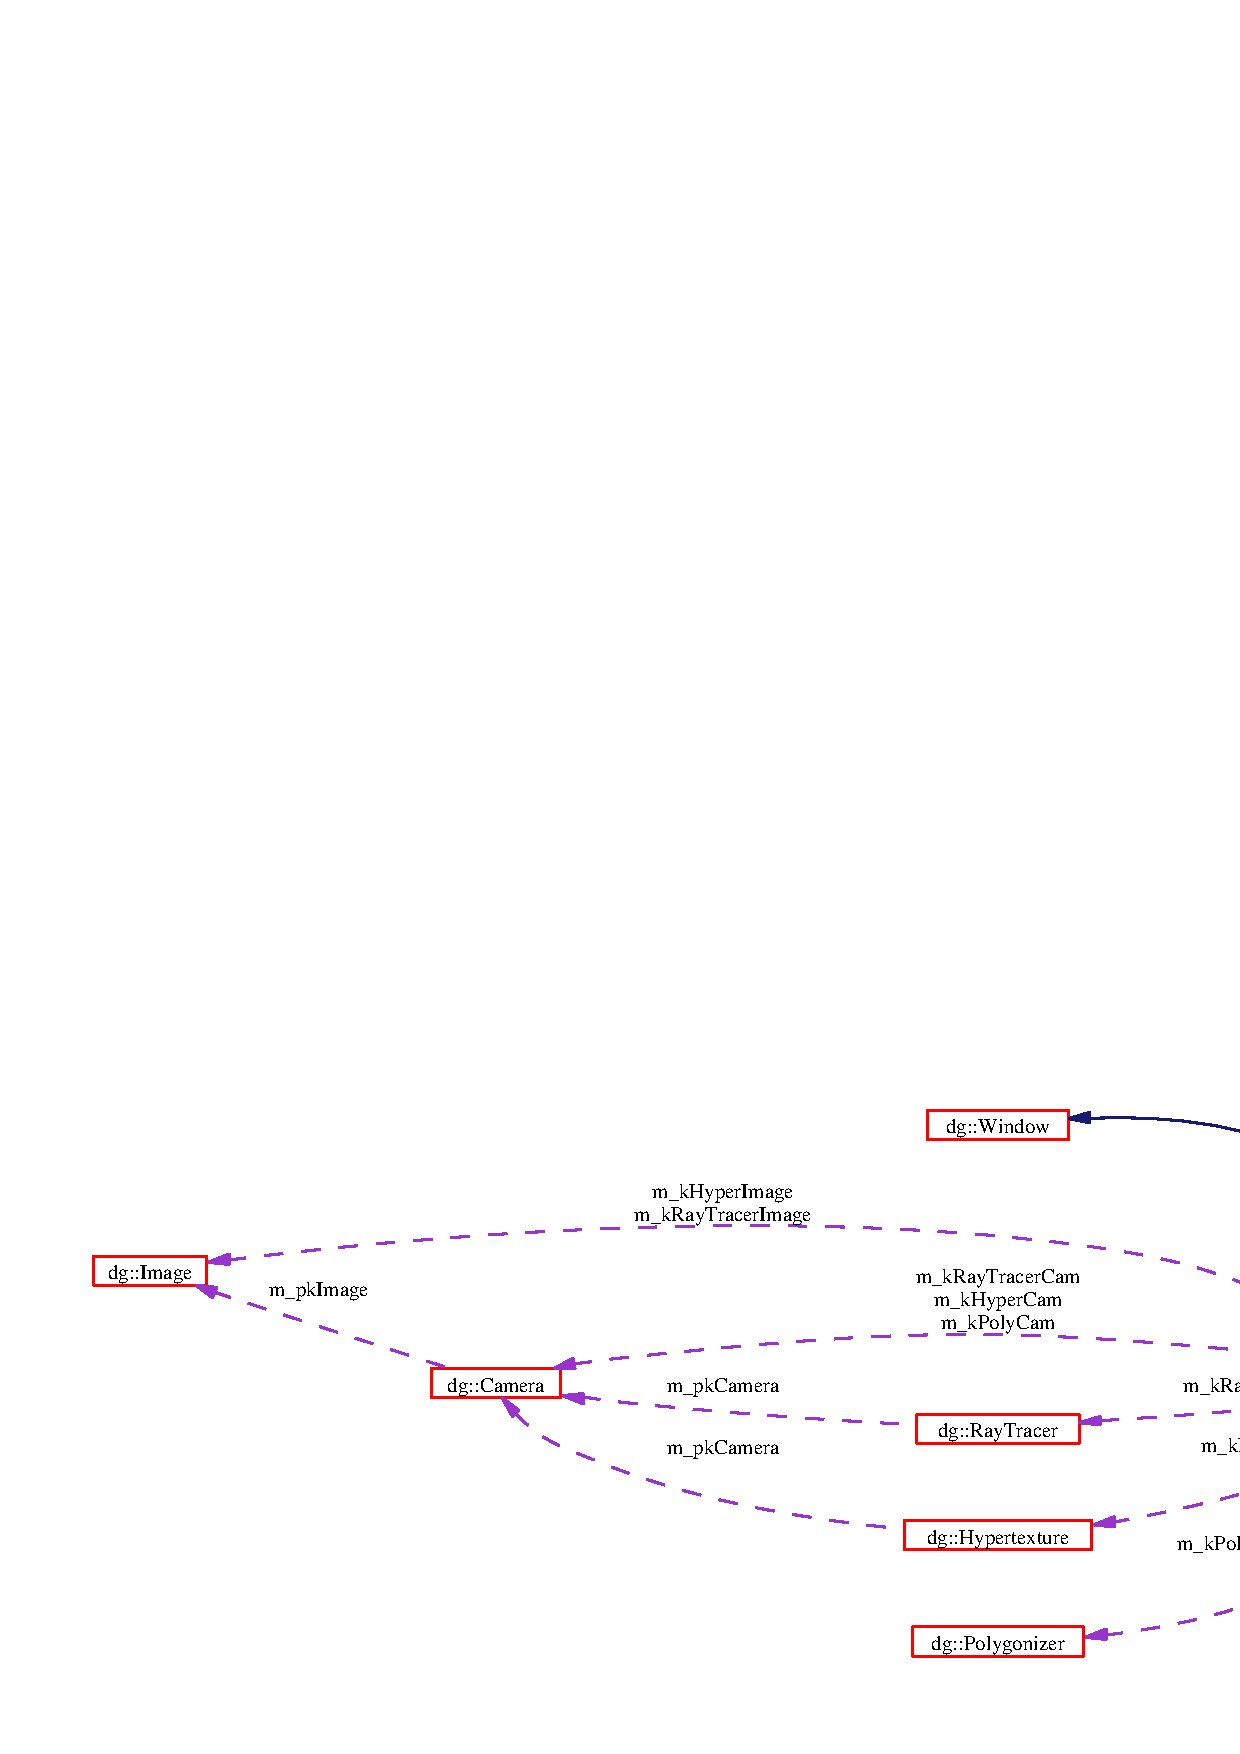
\includegraphics[width=372pt]{classdg_1_1Visualizer__coll__graph}
\end{center}
\end{figure}
\subsection*{Public Types}
\begin{CompactItemize}
\item 
enum {\bf Visualizer\-Mode} \{ {\bf VM\_\-MARCHING\_\-CUBES}, 
{\bf VM\_\-MARCHING\_\-TETRA}, 
{\bf VM\_\-RAYTRACE}, 
{\bf VM\_\-HYPERTEXTURE}, 
{\bf VM\_\-COUNT}
 \}
\end{CompactItemize}
\subsection*{Public Methods}
\begin{CompactItemize}
\item 
{\bf Visualizer} ()
\item 
virtual {\bf $\sim$Visualizer} ()
\item 
virtual {\bf Bool} {\bf on\-Startup} ()
\item 
virtual {\bf Bool} {\bf on\-Initialize} ()
\item 
virtual void {\bf on\-Reshape} ({\bf Int} i\-Width, {\bf Int} i\-Height)
\item 
virtual void {\bf on\-Display} ()
\item 
virtual void {\bf on\-Idle} ()
\item 
virtual void {\bf on\-Key\-Down} ({\bf UChar} uc\-Key, {\bf Int} i\-X, {\bf Int} i\-Y)
\item 
virtual void {\bf on\-Special\-Key\-Down} ({\bf Int} i\-Key, {\bf Int} i\-X, {\bf Int} i\-Y)
\item 
virtual void {\bf on\-Mouse\-Motion} ({\bf Int} i\-X, {\bf Int} i\-Y, {\bf UInt} ui\-Modifiers)
\item 
virtual void {\bf on\-Mouse\-Click} ({\bf Int} i\-Button, {\bf Int} i\-State, {\bf Int} i\-X, {\bf Int} i\-Y, {\bf UInt} ui\-Modifiers)
\item 
void {\bf draw\-Text} ()
\item 
void {\bf draw\-Polygons} ()
\item 
void {\bf draw\-Raytraced} ()
\item 
void {\bf draw\-Hypertexture} ()
\end{CompactItemize}
\subsection*{Protected Methods}
\begin{CompactItemize}
\item 
void {\bf setup\-Polygonizer} ()
\item 
void {\bf setup\-Ray\-Tracer} ()
\item 
void {\bf setup\-Hypertexture} ()
\item 
void {\bf setup\-Camera} ({\bf Camera} \&rk\-Camera)
\item 
void {\bf setup\-Frustum} ({\bf Int} i\-Width, {\bf Int} i\-Height, bool b\-Perspective)
\item 
void {\bf set\-Background} ()
\item 
void {\bf set\-Lights} ()
\item 
void {\bf set\-Materials} ()
\item 
void {\bf start\-Calc\-Timer} ()
\item 
void {\bf update\-Calc\-Timer} ()
\item 
void {\bf stop\-Calc\-Timer} ()
\item 
void {\bf update} ({\bf Real} f\-Time)
\end{CompactItemize}
\subsection*{Protected Attributes}
\begin{CompactItemize}
\item 
{\bf Real} {\bf m\_\-f\-Last\-Calc\-Time}
\item 
{\bf UInt} {\bf m\_\-ui\-Hours}
\item 
{\bf UInt} {\bf m\_\-ui\-Minutes}
\item 
{\bf UInt} {\bf m\_\-ui\-Seconds}
\item 
{\bf UInt} {\bf m\_\-ui\-Milli\-Secs}
\item 
bool {\bf m\_\-b\-Use\-Perspective}
\item 
bool {\bf m\_\-b\-Show\-Info}
\item 
bool {\bf m\_\-b\-Update}
\item 
bool {\bf m\_\-b\-Rotate}
\item 
bool {\bf m\_\-b\-Show\-Bounds}
\item 
bool {\bf m\_\-b\-Spin}
\item 
bool {\bf m\_\-b\-Move}
\item 
bool {\bf m\_\-b\-Light}
\item 
bool {\bf m\_\-b\-Rendering}
\item 
bool {\bf m\_\-b\-Ray\-Traced}
\item 
bool {\bf m\_\-b\-Hyper\-Traced}
\item 
bool {\bf m\_\-b\-Polygonized}
\item 
bool {\bf m\_\-b\-Keep\-In\-View}
\item 
bool {\bf m\_\-b\-Fade\-Out}
\item 
{\bf Int} {\bf m\_\-i\-Spin\-X}
\item 
{\bf Int} {\bf m\_\-i\-Spin\-Y}
\item 
{\bf Int} {\bf m\_\-i\-Orig\-X}
\item 
{\bf Int} {\bf m\_\-i\-Orig\-Y}
\item 
{\bf Int} {\bf m\_\-i\-Cell\-Count}
\item 
{\bf Real} {\bf m\_\-f\-Scale}
\item 
{\bf Real} {\bf m\_\-f\-Iso\-Level}
\item 
{\bf Real} {\bf m\_\-f\-Update\-Offset}
\item 
{\bf Real} {\bf m\_\-f\-Time}
\item 
{\bf Polygonizer::March\-Method} {\bf m\_\-e\-March\-Mode}
\item 
{\bf Real} {\bf m\_\-f\-Transparency}
\item 
{\bf Real} {\bf m\_\-f\-Offset\-X}
\item 
{\bf Real} {\bf m\_\-f\-Offset\-Y}
\item 
{\bf Real} {\bf m\_\-f\-Offset\-Z}
\item 
{\bf Real} {\bf m\_\-f\-Camera\-X}
\item 
{\bf Real} {\bf m\_\-f\-Camera\-Y}
\item 
{\bf Real} {\bf m\_\-f\-Camera\-Z}
\item 
{\bf Real} {\bf m\_\-f\-Frustum\-Left}
\item 
{\bf Real} {\bf m\_\-f\-Frustum\-Right}
\item 
{\bf Real} {\bf m\_\-f\-Frustum\-Bottom}
\item 
{\bf Real} {\bf m\_\-f\-Frustum\-Top}
\item 
{\bf Real} {\bf m\_\-f\-Frustum\-Near}
\item 
{\bf Real} {\bf m\_\-f\-Frustum\-Far}
\item 
{\bf Int} {\bf m\_\-e\-Poly\-Mode}
\item 
{\bf Polygonizer} {\bf m\_\-k\-Polygonizer}
\item 
{\bf Camera} {\bf m\_\-k\-Poly\-Cam}
\item 
{\bf Ray\-Tracer} {\bf m\_\-k\-Ray\-Tracer}
\item 
{\bf Camera} {\bf m\_\-k\-Ray\-Tracer\-Cam}
\item 
{\bf Image} {\bf m\_\-k\-Ray\-Tracer\-Image}
\item 
{\bf Hypertexture} {\bf m\_\-k\-Hyper}
\item 
{\bf Camera} {\bf m\_\-k\-Hyper\-Cam}
\item 
{\bf Image} {\bf m\_\-k\-Hyper\-Image}
\item 
{\bf UInt} {\bf m\_\-ui\-Func\-Index}
\item 
const char $\ast$ {\bf m\_\-auc\-Func\-Name}
\item 
{\bf Operator} {\bf m\_\-pv\-Function}
\item 
{\bf Visualizer\-Mode} {\bf m\_\-e\-Vis\-Mode}
\end{CompactItemize}
\subsection*{Static Protected Attributes}
\begin{CompactItemize}
\item 
const {\bf Real} {\bf ms\_\-f\-Cell\-To\-Ray\-Scale} = 2
\item 
const {\bf Real} {\bf ms\_\-f\-Cell\-To\-Hyper\-Step\-Scale} = 0.4
\end{CompactItemize}


\subsection{Member Enumeration Documentation}
\index{dg::Visualizer@{dg::Visualizer}!VisualizerMode@{VisualizerMode}}
\index{VisualizerMode@{VisualizerMode}!dg::Visualizer@{dg::Visualizer}}
\subsubsection{\setlength{\rightskip}{0pt plus 5cm}enum dg::Visualizer::Visualizer\-Mode}\label{classdg_1_1Visualizer_s5}


\begin{Desc}
\item[Enumeration values: ]\par
\begin{description}
\index{VM_MARCHING_CUBES@{VM\_\-MARCHING\_\-CUBES}!dg::Visualizer@{dg::Visualizer}}\index{dg::Visualizer@{dg::Visualizer}!VM_MARCHING_CUBES@{VM\_\-MARCHING\_\-CUBES}}\item[{\em 
{\em VM\_\-MARCHING\_\-CUBES}\label{classdg_1_1Visualizer_s5s0}
}]\index{VM_MARCHING_TETRA@{VM\_\-MARCHING\_\-TETRA}!dg::Visualizer@{dg::Visualizer}}\index{dg::Visualizer@{dg::Visualizer}!VM_MARCHING_TETRA@{VM\_\-MARCHING\_\-TETRA}}\item[{\em 
{\em VM\_\-MARCHING\_\-TETRA}\label{classdg_1_1Visualizer_s5s1}
}]\index{VM_RAYTRACE@{VM\_\-RAYTRACE}!dg::Visualizer@{dg::Visualizer}}\index{dg::Visualizer@{dg::Visualizer}!VM_RAYTRACE@{VM\_\-RAYTRACE}}\item[{\em 
{\em VM\_\-RAYTRACE}\label{classdg_1_1Visualizer_s5s2}
}]\index{VM_HYPERTEXTURE@{VM\_\-HYPERTEXTURE}!dg::Visualizer@{dg::Visualizer}}\index{dg::Visualizer@{dg::Visualizer}!VM_HYPERTEXTURE@{VM\_\-HYPERTEXTURE}}\item[{\em 
{\em VM\_\-HYPERTEXTURE}\label{classdg_1_1Visualizer_s5s3}
}]\index{VM_COUNT@{VM\_\-COUNT}!dg::Visualizer@{dg::Visualizer}}\index{dg::Visualizer@{dg::Visualizer}!VM_COUNT@{VM\_\-COUNT}}\item[{\em 
{\em VM\_\-COUNT}\label{classdg_1_1Visualizer_s5s4}
}]\end{description}
\end{Desc}



Definition at line 22 of file Visualizer.h.

\subsection{Constructor \& Destructor Documentation}
\index{dg::Visualizer@{dg::Visualizer}!Visualizer@{Visualizer}}
\index{Visualizer@{Visualizer}!dg::Visualizer@{dg::Visualizer}}
\subsubsection{\setlength{\rightskip}{0pt plus 5cm}Visualizer::Visualizer ()}\label{classdg_1_1Visualizer_a0}




Definition at line 16 of file Visualizer.cpp.\index{dg::Visualizer@{dg::Visualizer}!~Visualizer@{$\sim$Visualizer}}
\index{~Visualizer@{$\sim$Visualizer}!dg::Visualizer@{dg::Visualizer}}
\subsubsection{\setlength{\rightskip}{0pt plus 5cm}Visualizer::$\sim$Visualizer ()\hspace{0.3cm}{\tt  [virtual]}}\label{classdg_1_1Visualizer_a1}




Definition at line 23 of file Visualizer.cpp.

\subsection{Member Function Documentation}
\index{dg::Visualizer@{dg::Visualizer}!drawHypertexture@{drawHypertexture}}
\index{drawHypertexture@{drawHypertexture}!dg::Visualizer@{dg::Visualizer}}
\subsubsection{\setlength{\rightskip}{0pt plus 5cm}void Visualizer::draw\-Hypertexture ()}\label{classdg_1_1Visualizer_a14}




Definition at line 210 of file Visualizer.cpp.

References dg::Window::draw\-Image(), draw\-Text(), dg::Image::height(), m\_\-b\-Hyper\-Traced, m\_\-b\-Rendering, m\_\-b\-Update, m\_\-k\-Hyper, m\_\-k\-Hyper\-Image, dg::Image::pixels(), dg::Window::post\-Redisplay(), dg::Hypertexture::render(), set\-Background(), start\-Calc\-Timer(), stop\-Calc\-Timer(), dg::Window::swap\-Buffers(), dg::UInt, update\-Calc\-Timer(), and dg::Image::width().

Referenced by on\-Display().\index{dg::Visualizer@{dg::Visualizer}!drawPolygons@{drawPolygons}}
\index{drawPolygons@{drawPolygons}!dg::Visualizer@{dg::Visualizer}}
\subsubsection{\setlength{\rightskip}{0pt plus 5cm}void Visualizer::draw\-Polygons ()}\label{classdg_1_1Visualizer_a12}




Definition at line 269 of file Visualizer.cpp.

References dg::Polygonizer::evaluate(), dg::Polygonizer::get\-Colors(), dg::Camera::get\-Direction(), dg::Polygonizer::get\-Normals(), dg::Camera::get\-Position(), dg::Camera::get\-Up(), dg::Polygonizer::get\-Vertices(), m\_\-b\-Light, m\_\-b\-Polygonized, m\_\-b\-Update, m\_\-e\-March\-Mode, m\_\-k\-Poly\-Cam, m\_\-k\-Polygonizer, setup\-Camera(), start\-Calc\-Timer(), stop\-Calc\-Timer(), dg::UInt, dg::Vector::x(), dg::Vector::y(), and dg::Vector::z().

Referenced by on\-Display().\index{dg::Visualizer@{dg::Visualizer}!drawRaytraced@{drawRaytraced}}
\index{drawRaytraced@{drawRaytraced}!dg::Visualizer@{dg::Visualizer}}
\subsubsection{\setlength{\rightskip}{0pt plus 5cm}void Visualizer::draw\-Raytraced ()}\label{classdg_1_1Visualizer_a13}




Definition at line 151 of file Visualizer.cpp.

References dg::Window::draw\-Image(), draw\-Text(), dg::Image::height(), m\_\-b\-Ray\-Traced, m\_\-b\-Rendering, m\_\-b\-Update, m\_\-k\-Ray\-Tracer, m\_\-k\-Ray\-Tracer\-Image, dg::Image::pixels(), dg::Window::post\-Redisplay(), dg::Ray\-Tracer::render(), set\-Background(), start\-Calc\-Timer(), stop\-Calc\-Timer(), dg::Window::swap\-Buffers(), dg::UInt, update\-Calc\-Timer(), and dg::Image::width().

Referenced by on\-Display().\index{dg::Visualizer@{dg::Visualizer}!drawText@{drawText}}
\index{drawText@{drawText}!dg::Visualizer@{dg::Visualizer}}
\subsubsection{\setlength{\rightskip}{0pt plus 5cm}void Visualizer::draw\-Text ()}\label{classdg_1_1Visualizer_a11}




Definition at line 336 of file Visualizer.cpp.

References dg::Color::a(), dg::Color::b(), dg::Char, dg::Window::draw\-String(), dg::Color::g(), dg::Hypertexture::get\-Ray\-Hits(), dg::Ray\-Tracer::get\-Ray\-Hits(), dg::Hypertexture::get\-Samples(), dg::Hypertexture::get\-Step\-Size(), dg::Polygonizer::get\-Vertices(), dg::Window::height(), dg::Int, m\_\-auc\-Func\-Name, m\_\-e\-Vis\-Mode, m\_\-f\-Iso\-Level, m\_\-f\-Offset\-X, m\_\-f\-Offset\-Y, m\_\-f\-Offset\-Z, m\_\-f\-Scale, m\_\-i\-Cell\-Count, m\_\-i\-Spin\-X, m\_\-i\-Spin\-Y, m\_\-k\-Hyper, m\_\-k\-Polygonizer, m\_\-k\-Ray\-Tracer, m\_\-ui\-Hours, m\_\-ui\-Milli\-Secs, m\_\-ui\-Minutes, m\_\-ui\-Seconds, ms\_\-f\-Cell\-To\-Ray\-Scale, dg::Color::r(), dg::UInt, VM\_\-HYPERTEXTURE, VM\_\-MARCHING\_\-CUBES, VM\_\-MARCHING\_\-TETRA, VM\_\-RAYTRACE, and dg::Window::width().

Referenced by draw\-Hypertexture(), draw\-Raytraced(), and on\-Display().\index{dg::Visualizer@{dg::Visualizer}!onDisplay@{onDisplay}}
\index{onDisplay@{onDisplay}!dg::Visualizer@{dg::Visualizer}}
\subsubsection{\setlength{\rightskip}{0pt plus 5cm}void Visualizer::on\-Display ()\hspace{0.3cm}{\tt  [virtual]}}\label{classdg_1_1Visualizer_a5}




Reimplemented from {\bf dg::Window} {\rm (p.\,\pageref{classdg_1_1Window_a7})}.

Definition at line 125 of file Visualizer.cpp.

References draw\-Hypertexture(), draw\-Polygons(), draw\-Raytraced(), draw\-Text(), m\_\-b\-Update, m\_\-e\-Vis\-Mode, m\_\-f\-Time, dg::Window::swap\-Buffers(), update(), dg::Window::update\-Clicks(), VM\_\-HYPERTEXTURE, VM\_\-MARCHING\_\-CUBES, VM\_\-MARCHING\_\-TETRA, and VM\_\-RAYTRACE.

Referenced by on\-Idle().\index{dg::Visualizer@{dg::Visualizer}!onIdle@{onIdle}}
\index{onIdle@{onIdle}!dg::Visualizer@{dg::Visualizer}}
\subsubsection{\setlength{\rightskip}{0pt plus 5cm}virtual void dg::Visualizer::on\-Idle ()\hspace{0.3cm}{\tt  [inline, virtual]}}\label{classdg_1_1Visualizer_a6}




Reimplemented from {\bf dg::Window} {\rm (p.\,\pageref{classdg_1_1Window_a17})}.

Definition at line 41 of file Visualizer.h.

References on\-Display().\index{dg::Visualizer@{dg::Visualizer}!onInitialize@{onInitialize}}
\index{onInitialize@{onInitialize}!dg::Visualizer@{dg::Visualizer}}
\subsubsection{\setlength{\rightskip}{0pt plus 5cm}{\bf Bool} Visualizer::on\-Initialize ()\hspace{0.3cm}{\tt  [virtual]}}\label{classdg_1_1Visualizer_a3}




Reimplemented from {\bf dg::Window} {\rm (p.\,\pageref{classdg_1_1Window_a2})}.

Definition at line 85 of file Visualizer.cpp.

References dg::Bool, dg::Window::height(), on\-Reshape(), set\-Background(), set\-Lights(), set\-Materials(), setup\-Polygonizer(), and dg::Window::width().\index{dg::Visualizer@{dg::Visualizer}!onKeyDown@{onKeyDown}}
\index{onKeyDown@{onKeyDown}!dg::Visualizer@{dg::Visualizer}}
\subsubsection{\setlength{\rightskip}{0pt plus 5cm}void Visualizer::on\-Key\-Down ({\bf UChar} {\em uc\-Key}, {\bf Int} {\em i\-X}, {\bf Int} {\em i\-Y})\hspace{0.3cm}{\tt  [virtual]}}\label{classdg_1_1Visualizer_a7}




Reimplemented from {\bf dg::Window} {\rm (p.\,\pageref{classdg_1_1Window_a10})}.

Definition at line 504 of file Visualizer.cpp.

References dg::Window::height(), dg::Int, m\_\-b\-Fade\-Out, m\_\-b\-Hyper\-Traced, m\_\-b\-Keep\-In\-View, m\_\-b\-Light, m\_\-b\-Move, m\_\-b\-Polygonized, m\_\-b\-Ray\-Traced, m\_\-b\-Show\-Bounds, m\_\-b\-Show\-Info, m\_\-b\-Update, m\_\-b\-Use\-Perspective, m\_\-e\-March\-Mode, m\_\-e\-Poly\-Mode, m\_\-e\-Vis\-Mode, m\_\-f\-Camera\-Z, m\_\-f\-Frustum\-Far, m\_\-f\-Scale, m\_\-f\-Transparency, m\_\-i\-Cell\-Count, m\_\-k\-Polygonizer, m\_\-ui\-Func\-Index, on\-Reshape(), dg::Random\-Int(), dg::Polygonizer::set\-Cell\-Count(), set\-Materials(), dg::Polygonizer::set\-Scale(), setup\-Hypertexture(), setup\-Polygonizer(), setup\-Ray\-Tracer(), dg::UChar, dg::UInt, VM\_\-HYPERTEXTURE, VM\_\-MARCHING\_\-CUBES, VM\_\-MARCHING\_\-TETRA, VM\_\-RAYTRACE, and dg::Window::width().\index{dg::Visualizer@{dg::Visualizer}!onMouseClick@{onMouseClick}}
\index{onMouseClick@{onMouseClick}!dg::Visualizer@{dg::Visualizer}}
\subsubsection{\setlength{\rightskip}{0pt plus 5cm}void Visualizer::on\-Mouse\-Click ({\bf Int} {\em i\-Button}, {\bf Int} {\em i\-State}, {\bf Int} {\em i\-X}, {\bf Int} {\em i\-Y}, {\bf UInt} {\em ui\-Modifiers})\hspace{0.3cm}{\tt  [virtual]}}\label{classdg_1_1Visualizer_a10}




Reimplemented from {\bf dg::Window} {\rm (p.\,\pageref{classdg_1_1Window_a16})}.

Definition at line 483 of file Visualizer.cpp.

References dg::Int, dg::Window::m\_\-b\-Left\-Mouse\-Pressed, dg::Window::m\_\-b\-Middle\-Mouse\-Pressed, dg::Window::m\_\-b\-Right\-Mouse\-Pressed, m\_\-b\-Rotate, m\_\-e\-Vis\-Mode, m\_\-i\-Orig\-X, m\_\-i\-Orig\-Y, dg::UInt, VM\_\-HYPERTEXTURE, VM\_\-MARCHING\_\-TETRA, and VM\_\-RAYTRACE.\index{dg::Visualizer@{dg::Visualizer}!onMouseMotion@{onMouseMotion}}
\index{onMouseMotion@{onMouseMotion}!dg::Visualizer@{dg::Visualizer}}
\subsubsection{\setlength{\rightskip}{0pt plus 5cm}void Visualizer::on\-Mouse\-Motion ({\bf Int} {\em i\-X}, {\bf Int} {\em i\-Y}, {\bf UInt} {\em ui\-Modifiers})\hspace{0.3cm}{\tt  [virtual]}}\label{classdg_1_1Visualizer_a9}




Reimplemented from {\bf dg::Window} {\rm (p.\,\pageref{classdg_1_1Window_a15})}.

Definition at line 471 of file Visualizer.cpp.

References dg::Int, m\_\-i\-Orig\-X, m\_\-i\-Orig\-Y, m\_\-i\-Spin\-X, m\_\-i\-Spin\-Y, and dg::UInt.\index{dg::Visualizer@{dg::Visualizer}!onReshape@{onReshape}}
\index{onReshape@{onReshape}!dg::Visualizer@{dg::Visualizer}}
\subsubsection{\setlength{\rightskip}{0pt plus 5cm}void Visualizer::on\-Reshape ({\bf Int} {\em i\-Width}, {\bf Int} {\em i\-Height})\hspace{0.3cm}{\tt  [virtual]}}\label{classdg_1_1Visualizer_a4}




Reimplemented from {\bf dg::Window} {\rm (p.\,\pageref{classdg_1_1Window_a5})}.

Definition at line 98 of file Visualizer.cpp.

References dg::Int, m\_\-b\-Use\-Perspective, m\_\-f\-Frustum\-Bottom, m\_\-f\-Frustum\-Far, m\_\-f\-Frustum\-Left, m\_\-f\-Frustum\-Near, m\_\-f\-Frustum\-Right, m\_\-f\-Frustum\-Top, and setup\-Frustum().

Referenced by on\-Initialize(), and on\-Key\-Down().\index{dg::Visualizer@{dg::Visualizer}!onSpecialKeyDown@{onSpecialKeyDown}}
\index{onSpecialKeyDown@{onSpecialKeyDown}!dg::Visualizer@{dg::Visualizer}}
\subsubsection{\setlength{\rightskip}{0pt plus 5cm}void Visualizer::on\-Special\-Key\-Down ({\bf Int} {\em i\-Key}, {\bf Int} {\em i\-X}, {\bf Int} {\em i\-Y})\hspace{0.3cm}{\tt  [virtual]}}\label{classdg_1_1Visualizer_a8}




Reimplemented from {\bf dg::Window} {\rm (p.\,\pageref{classdg_1_1Window_a12})}.

Definition at line 669 of file Visualizer.cpp.

References dg::Int, m\_\-f\-Iso\-Level, m\_\-f\-Offset\-X, m\_\-f\-Offset\-Y, m\_\-f\-Offset\-Z, m\_\-k\-Polygonizer, dg::Polygonizer::set\-Iso\-Level(), dg::Polygonizer::set\-Offset(), and setup\-Polygonizer().\index{dg::Visualizer@{dg::Visualizer}!onStartup@{onStartup}}
\index{onStartup@{onStartup}!dg::Visualizer@{dg::Visualizer}}
\subsubsection{\setlength{\rightskip}{0pt plus 5cm}{\bf Bool} Visualizer::on\-Startup ()\hspace{0.3cm}{\tt  [virtual]}}\label{classdg_1_1Visualizer_a2}




Reimplemented from {\bf dg::Window} {\rm (p.\,\pageref{classdg_1_1Window_a1})}.

Definition at line 28 of file Visualizer.cpp.

References dg::Bool, dg::Camera::get\-Direction(), m\_\-auc\-Func\-Name, m\_\-b\-Fade\-Out, m\_\-b\-Hyper\-Traced, m\_\-b\-Keep\-In\-View, m\_\-b\-Light, m\_\-b\-Move, m\_\-b\-Polygonized, m\_\-b\-Ray\-Traced, m\_\-b\-Rotate, m\_\-b\-Show\-Bounds, m\_\-b\-Show\-Info, m\_\-b\-Spin, m\_\-b\-Update, m\_\-b\-Use\-Perspective, m\_\-e\-March\-Mode, m\_\-e\-Poly\-Mode, m\_\-f\-Camera\-X, m\_\-f\-Camera\-Y, m\_\-f\-Camera\-Z, m\_\-f\-Iso\-Level, m\_\-f\-Offset\-X, m\_\-f\-Offset\-Y, m\_\-f\-Offset\-Z, m\_\-f\-Scale, m\_\-f\-Time, m\_\-f\-Transparency, m\_\-i\-Cell\-Count, m\_\-i\-Orig\-X, m\_\-i\-Orig\-Y, m\_\-i\-Spin\-X, m\_\-i\-Spin\-Y, m\_\-k\-Hyper, m\_\-k\-Hyper\-Cam, m\_\-k\-Ray\-Tracer, m\_\-k\-Ray\-Tracer\-Cam, m\_\-pv\-Function, m\_\-ui\-Func\-Index, dg::Hypertexture::set\-Camera(), dg::Ray\-Tracer::set\-Camera(), dg::Hypertexture::set\-Density\-Function(), dg::Ray\-Tracer::set\-Function(), dg::Hypertexture::set\-Light\-Direction(), and dg::Ray\-Tracer::set\-Light\-Direction().\index{dg::Visualizer@{dg::Visualizer}!setBackground@{setBackground}}
\index{setBackground@{setBackground}!dg::Visualizer@{dg::Visualizer}}
\subsubsection{\setlength{\rightskip}{0pt plus 5cm}void Visualizer::set\-Background ()\hspace{0.3cm}{\tt  [protected]}}\label{classdg_1_1Visualizer_b5}




Definition at line 836 of file Visualizer.cpp.

References dg::Real.

Referenced by draw\-Hypertexture(), draw\-Raytraced(), and on\-Initialize().\index{dg::Visualizer@{dg::Visualizer}!setLights@{setLights}}
\index{setLights@{setLights}!dg::Visualizer@{dg::Visualizer}}
\subsubsection{\setlength{\rightskip}{0pt plus 5cm}void Visualizer::set\-Lights ()\hspace{0.3cm}{\tt  [protected]}}\label{classdg_1_1Visualizer_b6}




Definition at line 851 of file Visualizer.cpp.

References m\_\-e\-Poly\-Mode, and dg::Real.

Referenced by on\-Initialize().\index{dg::Visualizer@{dg::Visualizer}!setMaterials@{setMaterials}}
\index{setMaterials@{setMaterials}!dg::Visualizer@{dg::Visualizer}}
\subsubsection{\setlength{\rightskip}{0pt plus 5cm}void Visualizer::set\-Materials ()\hspace{0.3cm}{\tt  [protected]}}\label{classdg_1_1Visualizer_b7}




Definition at line 869 of file Visualizer.cpp.

References m\_\-f\-Transparency, and dg::Real.

Referenced by on\-Initialize(), and on\-Key\-Down().\index{dg::Visualizer@{dg::Visualizer}!setupCamera@{setupCamera}}
\index{setupCamera@{setupCamera}!dg::Visualizer@{dg::Visualizer}}
\subsubsection{\setlength{\rightskip}{0pt plus 5cm}void Visualizer::setup\-Camera ({\bf Camera} \& {\em rk\-Camera})\hspace{0.3cm}{\tt  [protected]}}\label{classdg_1_1Visualizer_b3}




Definition at line 894 of file Visualizer.cpp.

References dg::Camera::get\-Direction(), dg::Camera::get\-Position(), dg::Camera::get\-Up(), dg::Window::height(), dg::Vector::length(), m\_\-b\-Use\-Perspective, m\_\-f\-Camera\-X, m\_\-f\-Camera\-Y, m\_\-f\-Camera\-Z, m\_\-f\-Frustum\-Bottom, m\_\-f\-Frustum\-Far, m\_\-f\-Frustum\-Left, m\_\-f\-Frustum\-Near, m\_\-f\-Frustum\-Right, m\_\-f\-Frustum\-Top, m\_\-f\-Offset\-X, m\_\-f\-Offset\-Y, m\_\-f\-Offset\-Z, m\_\-f\-Scale, m\_\-i\-Spin\-X, m\_\-i\-Spin\-Y, m\_\-k\-Poly\-Cam, dg::Real, dg::Camera::set\-Direction(), dg::Camera::set\-Far(), dg::Camera::set\-Half\-Height(), dg::Camera::set\-Half\-Width(), dg::Camera::set\-Near(), dg::Camera::set\-Position(), dg::Camera::set\-Right(), dg::Camera::set\-Up(), setup\-Frustum(), and dg::Window::width().

Referenced by draw\-Polygons(), setup\-Hypertexture(), and setup\-Ray\-Tracer().\index{dg::Visualizer@{dg::Visualizer}!setupFrustum@{setupFrustum}}
\index{setupFrustum@{setupFrustum}!dg::Visualizer@{dg::Visualizer}}
\subsubsection{\setlength{\rightskip}{0pt plus 5cm}void Visualizer::setup\-Frustum ({\bf Int} {\em i\-Width}, {\bf Int} {\em i\-Height}, bool {\em b\-Perspective})\hspace{0.3cm}{\tt  [protected]}}\label{classdg_1_1Visualizer_b4}




Definition at line 958 of file Visualizer.cpp.

References dg::Int, m\_\-f\-Frustum\-Bottom, m\_\-f\-Frustum\-Far, m\_\-f\-Frustum\-Left, m\_\-f\-Frustum\-Near, m\_\-f\-Frustum\-Right, m\_\-f\-Frustum\-Top, and dg::Real.

Referenced by on\-Reshape(), and setup\-Camera().\index{dg::Visualizer@{dg::Visualizer}!setupHypertexture@{setupHypertexture}}
\index{setupHypertexture@{setupHypertexture}!dg::Visualizer@{dg::Visualizer}}
\subsubsection{\setlength{\rightskip}{0pt plus 5cm}void Visualizer::setup\-Hypertexture ()\hspace{0.3cm}{\tt  [protected]}}\label{classdg_1_1Visualizer_b2}




Definition at line 798 of file Visualizer.cpp.

References dg::Filtered\-Clown\-Color\-Volume(), dg::Window::height(), m\_\-auc\-Func\-Name, m\_\-b\-Fade\-Out, m\_\-b\-Hyper\-Traced, m\_\-b\-Keep\-In\-View, m\_\-b\-Update, m\_\-f\-Scale, m\_\-i\-Cell\-Count, m\_\-k\-Hyper, m\_\-k\-Hyper\-Cam, m\_\-k\-Hyper\-Image, m\_\-pv\-Function, m\_\-ui\-Func\-Index, ms\_\-f\-Cell\-To\-Hyper\-Step\-Scale, dg::Window::post\-Redisplay(), dg::Image::resize(), dg::Hypertexture::set\-Density\-Function(), dg::Hypertexture::set\-Fade\-Out(), dg::Hypertexture::set\-Filtered\-Color\-Function(), dg::Camera::set\-Image(), dg::Hypertexture::set\-Keep\-In\-View(), dg::Hypertexture::set\-Scale(), dg::Hypertexture::set\-Step\-Size(), setup\-Camera(), and dg::Window::width().

Referenced by on\-Key\-Down(), and update().\index{dg::Visualizer@{dg::Visualizer}!setupPolygonizer@{setupPolygonizer}}
\index{setupPolygonizer@{setupPolygonizer}!dg::Visualizer@{dg::Visualizer}}
\subsubsection{\setlength{\rightskip}{0pt plus 5cm}void Visualizer::setup\-Polygonizer ()\hspace{0.3cm}{\tt  [protected]}}\label{classdg_1_1Visualizer_b0}




Definition at line 739 of file Visualizer.cpp.

References m\_\-auc\-Func\-Name, m\_\-b\-Polygonized, m\_\-b\-Update, m\_\-f\-Iso\-Level, m\_\-f\-Offset\-X, m\_\-f\-Offset\-Y, m\_\-f\-Offset\-Z, m\_\-f\-Scale, m\_\-i\-Cell\-Count, m\_\-k\-Polygonizer, m\_\-pv\-Function, m\_\-ui\-Func\-Index, dg::Window::post\-Redisplay(), dg::Polygonizer::set\-Cell\-Count(), dg::Polygonizer::set\-Function(), dg::Polygonizer::set\-Iso\-Level(), dg::Polygonizer::set\-Offset(), and dg::Polygonizer::set\-Scale().

Referenced by on\-Initialize(), on\-Key\-Down(), on\-Special\-Key\-Down(), and update().\index{dg::Visualizer@{dg::Visualizer}!setupRayTracer@{setupRayTracer}}
\index{setupRayTracer@{setupRayTracer}!dg::Visualizer@{dg::Visualizer}}
\subsubsection{\setlength{\rightskip}{0pt plus 5cm}void Visualizer::setup\-Ray\-Tracer ()\hspace{0.3cm}{\tt  [protected]}}\label{classdg_1_1Visualizer_b1}




Definition at line 758 of file Visualizer.cpp.

References dg::Window::bg(), dg::Camera::get\-Direction(), dg::Window::height(), m\_\-auc\-Func\-Name, m\_\-b\-Ray\-Traced, m\_\-b\-Update, m\_\-f\-Iso\-Level, m\_\-i\-Cell\-Count, m\_\-k\-Ray\-Tracer, m\_\-k\-Ray\-Tracer\-Cam, m\_\-k\-Ray\-Tracer\-Image, m\_\-pv\-Function, m\_\-ui\-Func\-Index, ms\_\-f\-Cell\-To\-Ray\-Scale, dg::Window::post\-Redisplay(), dg::Image::resize(), dg::Ray\-Tracer::set\-Base\-Color(), dg::Ray\-Tracer::set\-Blur(), dg::Image::set\-Clear\-Color(), dg::Ray\-Tracer::set\-Function(), dg::Camera::set\-Image(), dg::Ray\-Tracer::set\-Iso\-Level(), dg::Ray\-Tracer::set\-Light\-Direction(), dg::Ray\-Tracer::set\-Samples(), setup\-Camera(), dg::UInt, and dg::Window::width().

Referenced by on\-Key\-Down(), and update().\index{dg::Visualizer@{dg::Visualizer}!startCalcTimer@{startCalcTimer}}
\index{startCalcTimer@{startCalcTimer}!dg::Visualizer@{dg::Visualizer}}
\subsubsection{\setlength{\rightskip}{0pt plus 5cm}void Visualizer::start\-Calc\-Timer ()\hspace{0.3cm}{\tt  [protected]}}\label{classdg_1_1Visualizer_b8}




Definition at line 997 of file Visualizer.cpp.

References dg::Window::m\_\-k\-Timer, m\_\-ui\-Hours, m\_\-ui\-Milli\-Secs, m\_\-ui\-Minutes, m\_\-ui\-Seconds, dg::Timer::reset(), and dg::Timer::start().

Referenced by draw\-Hypertexture(), draw\-Polygons(), and draw\-Raytraced().\index{dg::Visualizer@{dg::Visualizer}!stopCalcTimer@{stopCalcTimer}}
\index{stopCalcTimer@{stopCalcTimer}!dg::Visualizer@{dg::Visualizer}}
\subsubsection{\setlength{\rightskip}{0pt plus 5cm}void Visualizer::stop\-Calc\-Timer ()\hspace{0.3cm}{\tt  [protected]}}\label{classdg_1_1Visualizer_b10}




Definition at line 1008 of file Visualizer.cpp.

References update\-Calc\-Timer().

Referenced by draw\-Hypertexture(), draw\-Polygons(), and draw\-Raytraced().\index{dg::Visualizer@{dg::Visualizer}!update@{update}}
\index{update@{update}!dg::Visualizer@{dg::Visualizer}}
\subsubsection{\setlength{\rightskip}{0pt plus 5cm}void Visualizer::update ({\bf Real} {\em f\-Time})\hspace{0.3cm}{\tt  [protected]}}\label{classdg_1_1Visualizer_b11}




Definition at line 1022 of file Visualizer.cpp.

References m\_\-e\-Vis\-Mode, m\_\-f\-Offset\-X, m\_\-f\-Offset\-Y, m\_\-f\-Offset\-Z, m\_\-f\-Time, m\_\-f\-Update\-Offset, dg::Real, setup\-Hypertexture(), setup\-Polygonizer(), setup\-Ray\-Tracer(), dg::Sine(), VM\_\-HYPERTEXTURE, VM\_\-MARCHING\_\-CUBES, VM\_\-MARCHING\_\-TETRA, and VM\_\-RAYTRACE.

Referenced by on\-Display().\index{dg::Visualizer@{dg::Visualizer}!updateCalcTimer@{updateCalcTimer}}
\index{updateCalcTimer@{updateCalcTimer}!dg::Visualizer@{dg::Visualizer}}
\subsubsection{\setlength{\rightskip}{0pt plus 5cm}void Visualizer::update\-Calc\-Timer ()\hspace{0.3cm}{\tt  [protected]}}\label{classdg_1_1Visualizer_b9}




Definition at line 1014 of file Visualizer.cpp.

References dg::Timer::elapsed\-Hours(), dg::Timer::elapsed\-Milliseconds(), dg::Timer::elapsed\-Minutes(), dg::Timer::elapsed\-Seconds(), dg::Window::m\_\-k\-Timer, m\_\-ui\-Hours, m\_\-ui\-Milli\-Secs, m\_\-ui\-Minutes, and m\_\-ui\-Seconds.

Referenced by draw\-Hypertexture(), draw\-Raytraced(), and stop\-Calc\-Timer().

\subsection{Member Data Documentation}
\index{dg::Visualizer@{dg::Visualizer}!m_aucFuncName@{m\_\-aucFuncName}}
\index{m_aucFuncName@{m\_\-aucFuncName}!dg::Visualizer@{dg::Visualizer}}
\subsubsection{\setlength{\rightskip}{0pt plus 5cm}const char$\ast$ dg::Visualizer::m\_\-auc\-Func\-Name\hspace{0.3cm}{\tt  [protected]}}\label{classdg_1_1Visualizer_n52}




Definition at line 172 of file Visualizer.h.

Referenced by draw\-Text(), on\-Startup(), setup\-Hypertexture(), setup\-Polygonizer(), and setup\-Ray\-Tracer().\index{dg::Visualizer@{dg::Visualizer}!m_bFadeOut@{m\_\-bFadeOut}}
\index{m_bFadeOut@{m\_\-bFadeOut}!dg::Visualizer@{dg::Visualizer}}
\subsubsection{\setlength{\rightskip}{0pt plus 5cm}bool dg::Visualizer::m\_\-b\-Fade\-Out\hspace{0.3cm}{\tt  [protected]}}\label{classdg_1_1Visualizer_n18}




Definition at line 116 of file Visualizer.h.

Referenced by on\-Key\-Down(), on\-Startup(), and setup\-Hypertexture().\index{dg::Visualizer@{dg::Visualizer}!m_bHyperTraced@{m\_\-bHyperTraced}}
\index{m_bHyperTraced@{m\_\-bHyperTraced}!dg::Visualizer@{dg::Visualizer}}
\subsubsection{\setlength{\rightskip}{0pt plus 5cm}bool dg::Visualizer::m\_\-b\-Hyper\-Traced\hspace{0.3cm}{\tt  [protected]}}\label{classdg_1_1Visualizer_n15}




Definition at line 113 of file Visualizer.h.

Referenced by draw\-Hypertexture(), on\-Key\-Down(), on\-Startup(), and setup\-Hypertexture().\index{dg::Visualizer@{dg::Visualizer}!m_bKeepInView@{m\_\-bKeepInView}}
\index{m_bKeepInView@{m\_\-bKeepInView}!dg::Visualizer@{dg::Visualizer}}
\subsubsection{\setlength{\rightskip}{0pt plus 5cm}bool dg::Visualizer::m\_\-b\-Keep\-In\-View\hspace{0.3cm}{\tt  [protected]}}\label{classdg_1_1Visualizer_n17}




Definition at line 115 of file Visualizer.h.

Referenced by on\-Key\-Down(), on\-Startup(), and setup\-Hypertexture().\index{dg::Visualizer@{dg::Visualizer}!m_bLight@{m\_\-bLight}}
\index{m_bLight@{m\_\-bLight}!dg::Visualizer@{dg::Visualizer}}
\subsubsection{\setlength{\rightskip}{0pt plus 5cm}bool dg::Visualizer::m\_\-b\-Light\hspace{0.3cm}{\tt  [protected]}}\label{classdg_1_1Visualizer_n12}




Definition at line 108 of file Visualizer.h.

Referenced by draw\-Polygons(), on\-Key\-Down(), and on\-Startup().\index{dg::Visualizer@{dg::Visualizer}!m_bMove@{m\_\-bMove}}
\index{m_bMove@{m\_\-bMove}!dg::Visualizer@{dg::Visualizer}}
\subsubsection{\setlength{\rightskip}{0pt plus 5cm}bool dg::Visualizer::m\_\-b\-Move\hspace{0.3cm}{\tt  [protected]}}\label{classdg_1_1Visualizer_n11}




Definition at line 105 of file Visualizer.h.

Referenced by on\-Key\-Down(), and on\-Startup().\index{dg::Visualizer@{dg::Visualizer}!m_bPolygonized@{m\_\-bPolygonized}}
\index{m_bPolygonized@{m\_\-bPolygonized}!dg::Visualizer@{dg::Visualizer}}
\subsubsection{\setlength{\rightskip}{0pt plus 5cm}bool dg::Visualizer::m\_\-b\-Polygonized\hspace{0.3cm}{\tt  [protected]}}\label{classdg_1_1Visualizer_n16}




Definition at line 114 of file Visualizer.h.

Referenced by draw\-Polygons(), on\-Key\-Down(), on\-Startup(), and setup\-Polygonizer().\index{dg::Visualizer@{dg::Visualizer}!m_bRayTraced@{m\_\-bRayTraced}}
\index{m_bRayTraced@{m\_\-bRayTraced}!dg::Visualizer@{dg::Visualizer}}
\subsubsection{\setlength{\rightskip}{0pt plus 5cm}bool dg::Visualizer::m\_\-b\-Ray\-Traced\hspace{0.3cm}{\tt  [protected]}}\label{classdg_1_1Visualizer_n14}




Definition at line 112 of file Visualizer.h.

Referenced by draw\-Raytraced(), on\-Key\-Down(), on\-Startup(), and setup\-Ray\-Tracer().\index{dg::Visualizer@{dg::Visualizer}!m_bRendering@{m\_\-bRendering}}
\index{m_bRendering@{m\_\-bRendering}!dg::Visualizer@{dg::Visualizer}}
\subsubsection{\setlength{\rightskip}{0pt plus 5cm}bool dg::Visualizer::m\_\-b\-Rendering\hspace{0.3cm}{\tt  [protected]}}\label{classdg_1_1Visualizer_n13}




Definition at line 111 of file Visualizer.h.

Referenced by draw\-Hypertexture(), and draw\-Raytraced().\index{dg::Visualizer@{dg::Visualizer}!m_bRotate@{m\_\-bRotate}}
\index{m_bRotate@{m\_\-bRotate}!dg::Visualizer@{dg::Visualizer}}
\subsubsection{\setlength{\rightskip}{0pt plus 5cm}bool dg::Visualizer::m\_\-b\-Rotate\hspace{0.3cm}{\tt  [protected]}}\label{classdg_1_1Visualizer_n8}




Definition at line 96 of file Visualizer.h.

Referenced by on\-Mouse\-Click(), and on\-Startup().\index{dg::Visualizer@{dg::Visualizer}!m_bShowBounds@{m\_\-bShowBounds}}
\index{m_bShowBounds@{m\_\-bShowBounds}!dg::Visualizer@{dg::Visualizer}}
\subsubsection{\setlength{\rightskip}{0pt plus 5cm}bool dg::Visualizer::m\_\-b\-Show\-Bounds\hspace{0.3cm}{\tt  [protected]}}\label{classdg_1_1Visualizer_n9}




Definition at line 99 of file Visualizer.h.

Referenced by on\-Key\-Down(), and on\-Startup().\index{dg::Visualizer@{dg::Visualizer}!m_bShowInfo@{m\_\-bShowInfo}}
\index{m_bShowInfo@{m\_\-bShowInfo}!dg::Visualizer@{dg::Visualizer}}
\subsubsection{\setlength{\rightskip}{0pt plus 5cm}bool dg::Visualizer::m\_\-b\-Show\-Info\hspace{0.3cm}{\tt  [protected]}}\label{classdg_1_1Visualizer_n6}




Definition at line 90 of file Visualizer.h.

Referenced by on\-Key\-Down(), and on\-Startup().\index{dg::Visualizer@{dg::Visualizer}!m_bSpin@{m\_\-bSpin}}
\index{m_bSpin@{m\_\-bSpin}!dg::Visualizer@{dg::Visualizer}}
\subsubsection{\setlength{\rightskip}{0pt plus 5cm}bool dg::Visualizer::m\_\-b\-Spin\hspace{0.3cm}{\tt  [protected]}}\label{classdg_1_1Visualizer_n10}




Definition at line 102 of file Visualizer.h.

Referenced by on\-Startup().\index{dg::Visualizer@{dg::Visualizer}!m_bUpdate@{m\_\-bUpdate}}
\index{m_bUpdate@{m\_\-bUpdate}!dg::Visualizer@{dg::Visualizer}}
\subsubsection{\setlength{\rightskip}{0pt plus 5cm}bool dg::Visualizer::m\_\-b\-Update\hspace{0.3cm}{\tt  [protected]}}\label{classdg_1_1Visualizer_n7}




Definition at line 93 of file Visualizer.h.

Referenced by draw\-Hypertexture(), draw\-Polygons(), draw\-Raytraced(), on\-Display(), on\-Key\-Down(), on\-Startup(), setup\-Hypertexture(), setup\-Polygonizer(), and setup\-Ray\-Tracer().\index{dg::Visualizer@{dg::Visualizer}!m_bUsePerspective@{m\_\-bUsePerspective}}
\index{m_bUsePerspective@{m\_\-bUsePerspective}!dg::Visualizer@{dg::Visualizer}}
\subsubsection{\setlength{\rightskip}{0pt plus 5cm}bool dg::Visualizer::m\_\-b\-Use\-Perspective\hspace{0.3cm}{\tt  [protected]}}\label{classdg_1_1Visualizer_n5}




Definition at line 87 of file Visualizer.h.

Referenced by on\-Key\-Down(), on\-Reshape(), on\-Startup(), and setup\-Camera().\index{dg::Visualizer@{dg::Visualizer}!m_eMarchMode@{m\_\-eMarchMode}}
\index{m_eMarchMode@{m\_\-eMarchMode}!dg::Visualizer@{dg::Visualizer}}
\subsubsection{\setlength{\rightskip}{0pt plus 5cm}{\bf Polygonizer::March\-Method} dg::Visualizer::m\_\-e\-March\-Mode\hspace{0.3cm}{\tt  [protected]}}\label{classdg_1_1Visualizer_n28}




Definition at line 130 of file Visualizer.h.

Referenced by draw\-Polygons(), on\-Key\-Down(), and on\-Startup().\index{dg::Visualizer@{dg::Visualizer}!m_ePolyMode@{m\_\-ePolyMode}}
\index{m_ePolyMode@{m\_\-ePolyMode}!dg::Visualizer@{dg::Visualizer}}
\subsubsection{\setlength{\rightskip}{0pt plus 5cm}{\bf Int} dg::Visualizer::m\_\-e\-Poly\-Mode\hspace{0.3cm}{\tt  [protected]}}\label{classdg_1_1Visualizer_n42}




Definition at line 154 of file Visualizer.h.

Referenced by on\-Key\-Down(), on\-Startup(), and set\-Lights().\index{dg::Visualizer@{dg::Visualizer}!m_eVisMode@{m\_\-eVisMode}}
\index{m_eVisMode@{m\_\-eVisMode}!dg::Visualizer@{dg::Visualizer}}
\subsubsection{\setlength{\rightskip}{0pt plus 5cm}{\bf Visualizer\-Mode} dg::Visualizer::m\_\-e\-Vis\-Mode\hspace{0.3cm}{\tt  [protected]}}\label{classdg_1_1Visualizer_n54}




Definition at line 176 of file Visualizer.h.

Referenced by draw\-Text(), on\-Display(), on\-Key\-Down(), on\-Mouse\-Click(), and update().\index{dg::Visualizer@{dg::Visualizer}!m_fCameraX@{m\_\-fCameraX}}
\index{m_fCameraX@{m\_\-fCameraX}!dg::Visualizer@{dg::Visualizer}}
\subsubsection{\setlength{\rightskip}{0pt plus 5cm}{\bf Real} dg::Visualizer::m\_\-f\-Camera\-X\hspace{0.3cm}{\tt  [protected]}}\label{classdg_1_1Visualizer_n33}




Definition at line 141 of file Visualizer.h.

Referenced by on\-Startup(), and setup\-Camera().\index{dg::Visualizer@{dg::Visualizer}!m_fCameraY@{m\_\-fCameraY}}
\index{m_fCameraY@{m\_\-fCameraY}!dg::Visualizer@{dg::Visualizer}}
\subsubsection{\setlength{\rightskip}{0pt plus 5cm}{\bf Real} dg::Visualizer::m\_\-f\-Camera\-Y\hspace{0.3cm}{\tt  [protected]}}\label{classdg_1_1Visualizer_n34}




Definition at line 142 of file Visualizer.h.

Referenced by on\-Startup(), and setup\-Camera().\index{dg::Visualizer@{dg::Visualizer}!m_fCameraZ@{m\_\-fCameraZ}}
\index{m_fCameraZ@{m\_\-fCameraZ}!dg::Visualizer@{dg::Visualizer}}
\subsubsection{\setlength{\rightskip}{0pt plus 5cm}{\bf Real} dg::Visualizer::m\_\-f\-Camera\-Z\hspace{0.3cm}{\tt  [protected]}}\label{classdg_1_1Visualizer_n35}




Definition at line 143 of file Visualizer.h.

Referenced by on\-Key\-Down(), on\-Startup(), and setup\-Camera().\index{dg::Visualizer@{dg::Visualizer}!m_fFrustumBottom@{m\_\-fFrustumBottom}}
\index{m_fFrustumBottom@{m\_\-fFrustumBottom}!dg::Visualizer@{dg::Visualizer}}
\subsubsection{\setlength{\rightskip}{0pt plus 5cm}{\bf Real} dg::Visualizer::m\_\-f\-Frustum\-Bottom\hspace{0.3cm}{\tt  [protected]}}\label{classdg_1_1Visualizer_n38}




Definition at line 148 of file Visualizer.h.

Referenced by on\-Reshape(), setup\-Camera(), and setup\-Frustum().\index{dg::Visualizer@{dg::Visualizer}!m_fFrustumFar@{m\_\-fFrustumFar}}
\index{m_fFrustumFar@{m\_\-fFrustumFar}!dg::Visualizer@{dg::Visualizer}}
\subsubsection{\setlength{\rightskip}{0pt plus 5cm}{\bf Real} dg::Visualizer::m\_\-f\-Frustum\-Far\hspace{0.3cm}{\tt  [protected]}}\label{classdg_1_1Visualizer_n41}




Definition at line 151 of file Visualizer.h.

Referenced by on\-Key\-Down(), on\-Reshape(), setup\-Camera(), and setup\-Frustum().\index{dg::Visualizer@{dg::Visualizer}!m_fFrustumLeft@{m\_\-fFrustumLeft}}
\index{m_fFrustumLeft@{m\_\-fFrustumLeft}!dg::Visualizer@{dg::Visualizer}}
\subsubsection{\setlength{\rightskip}{0pt plus 5cm}{\bf Real} dg::Visualizer::m\_\-f\-Frustum\-Left\hspace{0.3cm}{\tt  [protected]}}\label{classdg_1_1Visualizer_n36}




Definition at line 146 of file Visualizer.h.

Referenced by on\-Reshape(), setup\-Camera(), and setup\-Frustum().\index{dg::Visualizer@{dg::Visualizer}!m_fFrustumNear@{m\_\-fFrustumNear}}
\index{m_fFrustumNear@{m\_\-fFrustumNear}!dg::Visualizer@{dg::Visualizer}}
\subsubsection{\setlength{\rightskip}{0pt plus 5cm}{\bf Real} dg::Visualizer::m\_\-f\-Frustum\-Near\hspace{0.3cm}{\tt  [protected]}}\label{classdg_1_1Visualizer_n40}




Definition at line 150 of file Visualizer.h.

Referenced by on\-Reshape(), setup\-Camera(), and setup\-Frustum().\index{dg::Visualizer@{dg::Visualizer}!m_fFrustumRight@{m\_\-fFrustumRight}}
\index{m_fFrustumRight@{m\_\-fFrustumRight}!dg::Visualizer@{dg::Visualizer}}
\subsubsection{\setlength{\rightskip}{0pt plus 5cm}{\bf Real} dg::Visualizer::m\_\-f\-Frustum\-Right\hspace{0.3cm}{\tt  [protected]}}\label{classdg_1_1Visualizer_n37}




Definition at line 147 of file Visualizer.h.

Referenced by on\-Reshape(), setup\-Camera(), and setup\-Frustum().\index{dg::Visualizer@{dg::Visualizer}!m_fFrustumTop@{m\_\-fFrustumTop}}
\index{m_fFrustumTop@{m\_\-fFrustumTop}!dg::Visualizer@{dg::Visualizer}}
\subsubsection{\setlength{\rightskip}{0pt plus 5cm}{\bf Real} dg::Visualizer::m\_\-f\-Frustum\-Top\hspace{0.3cm}{\tt  [protected]}}\label{classdg_1_1Visualizer_n39}




Definition at line 149 of file Visualizer.h.

Referenced by on\-Reshape(), setup\-Camera(), and setup\-Frustum().\index{dg::Visualizer@{dg::Visualizer}!m_fIsoLevel@{m\_\-fIsoLevel}}
\index{m_fIsoLevel@{m\_\-fIsoLevel}!dg::Visualizer@{dg::Visualizer}}
\subsubsection{\setlength{\rightskip}{0pt plus 5cm}{\bf Real} dg::Visualizer::m\_\-f\-Iso\-Level\hspace{0.3cm}{\tt  [protected]}}\label{classdg_1_1Visualizer_n25}




Definition at line 127 of file Visualizer.h.

Referenced by draw\-Text(), on\-Special\-Key\-Down(), on\-Startup(), setup\-Polygonizer(), and setup\-Ray\-Tracer().\index{dg::Visualizer@{dg::Visualizer}!m_fLastCalcTime@{m\_\-fLastCalcTime}}
\index{m_fLastCalcTime@{m\_\-fLastCalcTime}!dg::Visualizer@{dg::Visualizer}}
\subsubsection{\setlength{\rightskip}{0pt plus 5cm}{\bf Real} dg::Visualizer::m\_\-f\-Last\-Calc\-Time\hspace{0.3cm}{\tt  [protected]}}\label{classdg_1_1Visualizer_n0}




Definition at line 80 of file Visualizer.h.\index{dg::Visualizer@{dg::Visualizer}!m_fOffsetX@{m\_\-fOffsetX}}
\index{m_fOffsetX@{m\_\-fOffsetX}!dg::Visualizer@{dg::Visualizer}}
\subsubsection{\setlength{\rightskip}{0pt plus 5cm}{\bf Real} dg::Visualizer::m\_\-f\-Offset\-X\hspace{0.3cm}{\tt  [protected]}}\label{classdg_1_1Visualizer_n30}




Definition at line 136 of file Visualizer.h.

Referenced by draw\-Text(), on\-Special\-Key\-Down(), on\-Startup(), setup\-Camera(), setup\-Polygonizer(), and update().\index{dg::Visualizer@{dg::Visualizer}!m_fOffsetY@{m\_\-fOffsetY}}
\index{m_fOffsetY@{m\_\-fOffsetY}!dg::Visualizer@{dg::Visualizer}}
\subsubsection{\setlength{\rightskip}{0pt plus 5cm}{\bf Real} dg::Visualizer::m\_\-f\-Offset\-Y\hspace{0.3cm}{\tt  [protected]}}\label{classdg_1_1Visualizer_n31}




Definition at line 137 of file Visualizer.h.

Referenced by draw\-Text(), on\-Special\-Key\-Down(), on\-Startup(), setup\-Camera(), setup\-Polygonizer(), and update().\index{dg::Visualizer@{dg::Visualizer}!m_fOffsetZ@{m\_\-fOffsetZ}}
\index{m_fOffsetZ@{m\_\-fOffsetZ}!dg::Visualizer@{dg::Visualizer}}
\subsubsection{\setlength{\rightskip}{0pt plus 5cm}{\bf Real} dg::Visualizer::m\_\-f\-Offset\-Z\hspace{0.3cm}{\tt  [protected]}}\label{classdg_1_1Visualizer_n32}




Definition at line 138 of file Visualizer.h.

Referenced by draw\-Text(), on\-Special\-Key\-Down(), on\-Startup(), setup\-Camera(), setup\-Polygonizer(), and update().\index{dg::Visualizer@{dg::Visualizer}!m_fScale@{m\_\-fScale}}
\index{m_fScale@{m\_\-fScale}!dg::Visualizer@{dg::Visualizer}}
\subsubsection{\setlength{\rightskip}{0pt plus 5cm}{\bf Real} dg::Visualizer::m\_\-f\-Scale\hspace{0.3cm}{\tt  [protected]}}\label{classdg_1_1Visualizer_n24}




Definition at line 126 of file Visualizer.h.

Referenced by draw\-Text(), on\-Key\-Down(), on\-Startup(), setup\-Camera(), setup\-Hypertexture(), and setup\-Polygonizer().\index{dg::Visualizer@{dg::Visualizer}!m_fTime@{m\_\-fTime}}
\index{m_fTime@{m\_\-fTime}!dg::Visualizer@{dg::Visualizer}}
\subsubsection{\setlength{\rightskip}{0pt plus 5cm}{\bf Real} dg::Visualizer::m\_\-f\-Time\hspace{0.3cm}{\tt  [protected]}}\label{classdg_1_1Visualizer_n27}




Definition at line 129 of file Visualizer.h.

Referenced by on\-Display(), on\-Startup(), and update().\index{dg::Visualizer@{dg::Visualizer}!m_fTransparency@{m\_\-fTransparency}}
\index{m_fTransparency@{m\_\-fTransparency}!dg::Visualizer@{dg::Visualizer}}
\subsubsection{\setlength{\rightskip}{0pt plus 5cm}{\bf Real} dg::Visualizer::m\_\-f\-Transparency\hspace{0.3cm}{\tt  [protected]}}\label{classdg_1_1Visualizer_n29}




Definition at line 133 of file Visualizer.h.

Referenced by on\-Key\-Down(), on\-Startup(), and set\-Materials().\index{dg::Visualizer@{dg::Visualizer}!m_fUpdateOffset@{m\_\-fUpdateOffset}}
\index{m_fUpdateOffset@{m\_\-fUpdateOffset}!dg::Visualizer@{dg::Visualizer}}
\subsubsection{\setlength{\rightskip}{0pt plus 5cm}{\bf Real} dg::Visualizer::m\_\-f\-Update\-Offset\hspace{0.3cm}{\tt  [protected]}}\label{classdg_1_1Visualizer_n26}




Definition at line 128 of file Visualizer.h.

Referenced by update().\index{dg::Visualizer@{dg::Visualizer}!m_iCellCount@{m\_\-iCellCount}}
\index{m_iCellCount@{m\_\-iCellCount}!dg::Visualizer@{dg::Visualizer}}
\subsubsection{\setlength{\rightskip}{0pt plus 5cm}{\bf Int} dg::Visualizer::m\_\-i\-Cell\-Count\hspace{0.3cm}{\tt  [protected]}}\label{classdg_1_1Visualizer_n23}




Definition at line 125 of file Visualizer.h.

Referenced by draw\-Text(), on\-Key\-Down(), on\-Startup(), setup\-Hypertexture(), setup\-Polygonizer(), and setup\-Ray\-Tracer().\index{dg::Visualizer@{dg::Visualizer}!m_iOrigX@{m\_\-iOrigX}}
\index{m_iOrigX@{m\_\-iOrigX}!dg::Visualizer@{dg::Visualizer}}
\subsubsection{\setlength{\rightskip}{0pt plus 5cm}{\bf Int} dg::Visualizer::m\_\-i\-Orig\-X\hspace{0.3cm}{\tt  [protected]}}\label{classdg_1_1Visualizer_n21}




Definition at line 121 of file Visualizer.h.

Referenced by on\-Mouse\-Click(), on\-Mouse\-Motion(), and on\-Startup().\index{dg::Visualizer@{dg::Visualizer}!m_iOrigY@{m\_\-iOrigY}}
\index{m_iOrigY@{m\_\-iOrigY}!dg::Visualizer@{dg::Visualizer}}
\subsubsection{\setlength{\rightskip}{0pt plus 5cm}{\bf Int} dg::Visualizer::m\_\-i\-Orig\-Y\hspace{0.3cm}{\tt  [protected]}}\label{classdg_1_1Visualizer_n22}




Definition at line 122 of file Visualizer.h.

Referenced by on\-Mouse\-Click(), on\-Mouse\-Motion(), and on\-Startup().\index{dg::Visualizer@{dg::Visualizer}!m_iSpinX@{m\_\-iSpinX}}
\index{m_iSpinX@{m\_\-iSpinX}!dg::Visualizer@{dg::Visualizer}}
\subsubsection{\setlength{\rightskip}{0pt plus 5cm}{\bf Int} dg::Visualizer::m\_\-i\-Spin\-X\hspace{0.3cm}{\tt  [protected]}}\label{classdg_1_1Visualizer_n19}




Definition at line 119 of file Visualizer.h.

Referenced by draw\-Text(), on\-Mouse\-Motion(), on\-Startup(), and setup\-Camera().\index{dg::Visualizer@{dg::Visualizer}!m_iSpinY@{m\_\-iSpinY}}
\index{m_iSpinY@{m\_\-iSpinY}!dg::Visualizer@{dg::Visualizer}}
\subsubsection{\setlength{\rightskip}{0pt plus 5cm}{\bf Int} dg::Visualizer::m\_\-i\-Spin\-Y\hspace{0.3cm}{\tt  [protected]}}\label{classdg_1_1Visualizer_n20}




Definition at line 120 of file Visualizer.h.

Referenced by draw\-Text(), on\-Mouse\-Motion(), on\-Startup(), and setup\-Camera().\index{dg::Visualizer@{dg::Visualizer}!m_kHyper@{m\_\-kHyper}}
\index{m_kHyper@{m\_\-kHyper}!dg::Visualizer@{dg::Visualizer}}
\subsubsection{\setlength{\rightskip}{0pt plus 5cm}{\bf Hypertexture} dg::Visualizer::m\_\-k\-Hyper\hspace{0.3cm}{\tt  [protected]}}\label{classdg_1_1Visualizer_n48}




Definition at line 166 of file Visualizer.h.

Referenced by draw\-Hypertexture(), draw\-Text(), on\-Startup(), and setup\-Hypertexture().\index{dg::Visualizer@{dg::Visualizer}!m_kHyperCam@{m\_\-kHyperCam}}
\index{m_kHyperCam@{m\_\-kHyperCam}!dg::Visualizer@{dg::Visualizer}}
\subsubsection{\setlength{\rightskip}{0pt plus 5cm}{\bf Camera} dg::Visualizer::m\_\-k\-Hyper\-Cam\hspace{0.3cm}{\tt  [protected]}}\label{classdg_1_1Visualizer_n49}




Definition at line 167 of file Visualizer.h.

Referenced by on\-Startup(), and setup\-Hypertexture().\index{dg::Visualizer@{dg::Visualizer}!m_kHyperImage@{m\_\-kHyperImage}}
\index{m_kHyperImage@{m\_\-kHyperImage}!dg::Visualizer@{dg::Visualizer}}
\subsubsection{\setlength{\rightskip}{0pt plus 5cm}{\bf Image} dg::Visualizer::m\_\-k\-Hyper\-Image\hspace{0.3cm}{\tt  [protected]}}\label{classdg_1_1Visualizer_n50}




Definition at line 168 of file Visualizer.h.

Referenced by draw\-Hypertexture(), and setup\-Hypertexture().\index{dg::Visualizer@{dg::Visualizer}!m_kPolyCam@{m\_\-kPolyCam}}
\index{m_kPolyCam@{m\_\-kPolyCam}!dg::Visualizer@{dg::Visualizer}}
\subsubsection{\setlength{\rightskip}{0pt plus 5cm}{\bf Camera} dg::Visualizer::m\_\-k\-Poly\-Cam\hspace{0.3cm}{\tt  [protected]}}\label{classdg_1_1Visualizer_n44}




Definition at line 158 of file Visualizer.h.

Referenced by draw\-Polygons(), and setup\-Camera().\index{dg::Visualizer@{dg::Visualizer}!m_kPolygonizer@{m\_\-kPolygonizer}}
\index{m_kPolygonizer@{m\_\-kPolygonizer}!dg::Visualizer@{dg::Visualizer}}
\subsubsection{\setlength{\rightskip}{0pt plus 5cm}{\bf Polygonizer} dg::Visualizer::m\_\-k\-Polygonizer\hspace{0.3cm}{\tt  [protected]}}\label{classdg_1_1Visualizer_n43}




Definition at line 157 of file Visualizer.h.

Referenced by draw\-Polygons(), draw\-Text(), on\-Key\-Down(), on\-Special\-Key\-Down(), and setup\-Polygonizer().\index{dg::Visualizer@{dg::Visualizer}!m_kRayTracer@{m\_\-kRayTracer}}
\index{m_kRayTracer@{m\_\-kRayTracer}!dg::Visualizer@{dg::Visualizer}}
\subsubsection{\setlength{\rightskip}{0pt plus 5cm}{\bf Ray\-Tracer} dg::Visualizer::m\_\-k\-Ray\-Tracer\hspace{0.3cm}{\tt  [protected]}}\label{classdg_1_1Visualizer_n45}




Definition at line 161 of file Visualizer.h.

Referenced by draw\-Raytraced(), draw\-Text(), on\-Startup(), and setup\-Ray\-Tracer().\index{dg::Visualizer@{dg::Visualizer}!m_kRayTracerCam@{m\_\-kRayTracerCam}}
\index{m_kRayTracerCam@{m\_\-kRayTracerCam}!dg::Visualizer@{dg::Visualizer}}
\subsubsection{\setlength{\rightskip}{0pt plus 5cm}{\bf Camera} dg::Visualizer::m\_\-k\-Ray\-Tracer\-Cam\hspace{0.3cm}{\tt  [protected]}}\label{classdg_1_1Visualizer_n46}




Definition at line 162 of file Visualizer.h.

Referenced by on\-Startup(), and setup\-Ray\-Tracer().\index{dg::Visualizer@{dg::Visualizer}!m_kRayTracerImage@{m\_\-kRayTracerImage}}
\index{m_kRayTracerImage@{m\_\-kRayTracerImage}!dg::Visualizer@{dg::Visualizer}}
\subsubsection{\setlength{\rightskip}{0pt plus 5cm}{\bf Image} dg::Visualizer::m\_\-k\-Ray\-Tracer\-Image\hspace{0.3cm}{\tt  [protected]}}\label{classdg_1_1Visualizer_n47}




Definition at line 163 of file Visualizer.h.

Referenced by draw\-Raytraced(), and setup\-Ray\-Tracer().\index{dg::Visualizer@{dg::Visualizer}!m_pvFunction@{m\_\-pvFunction}}
\index{m_pvFunction@{m\_\-pvFunction}!dg::Visualizer@{dg::Visualizer}}
\subsubsection{\setlength{\rightskip}{0pt plus 5cm}{\bf Operator} dg::Visualizer::m\_\-pv\-Function\hspace{0.3cm}{\tt  [protected]}}\label{classdg_1_1Visualizer_n53}




Definition at line 173 of file Visualizer.h.

Referenced by on\-Startup(), setup\-Hypertexture(), setup\-Polygonizer(), and setup\-Ray\-Tracer().\index{dg::Visualizer@{dg::Visualizer}!m_uiFuncIndex@{m\_\-uiFuncIndex}}
\index{m_uiFuncIndex@{m\_\-uiFuncIndex}!dg::Visualizer@{dg::Visualizer}}
\subsubsection{\setlength{\rightskip}{0pt plus 5cm}{\bf UInt} dg::Visualizer::m\_\-ui\-Func\-Index\hspace{0.3cm}{\tt  [protected]}}\label{classdg_1_1Visualizer_n51}




Definition at line 171 of file Visualizer.h.

Referenced by on\-Key\-Down(), on\-Startup(), setup\-Hypertexture(), setup\-Polygonizer(), and setup\-Ray\-Tracer().\index{dg::Visualizer@{dg::Visualizer}!m_uiHours@{m\_\-uiHours}}
\index{m_uiHours@{m\_\-uiHours}!dg::Visualizer@{dg::Visualizer}}
\subsubsection{\setlength{\rightskip}{0pt plus 5cm}{\bf UInt} dg::Visualizer::m\_\-ui\-Hours\hspace{0.3cm}{\tt  [protected]}}\label{classdg_1_1Visualizer_n1}




Definition at line 81 of file Visualizer.h.

Referenced by draw\-Text(), start\-Calc\-Timer(), and update\-Calc\-Timer().\index{dg::Visualizer@{dg::Visualizer}!m_uiMilliSecs@{m\_\-uiMilliSecs}}
\index{m_uiMilliSecs@{m\_\-uiMilliSecs}!dg::Visualizer@{dg::Visualizer}}
\subsubsection{\setlength{\rightskip}{0pt plus 5cm}{\bf UInt} dg::Visualizer::m\_\-ui\-Milli\-Secs\hspace{0.3cm}{\tt  [protected]}}\label{classdg_1_1Visualizer_n4}




Definition at line 84 of file Visualizer.h.

Referenced by draw\-Text(), start\-Calc\-Timer(), and update\-Calc\-Timer().\index{dg::Visualizer@{dg::Visualizer}!m_uiMinutes@{m\_\-uiMinutes}}
\index{m_uiMinutes@{m\_\-uiMinutes}!dg::Visualizer@{dg::Visualizer}}
\subsubsection{\setlength{\rightskip}{0pt plus 5cm}{\bf UInt} dg::Visualizer::m\_\-ui\-Minutes\hspace{0.3cm}{\tt  [protected]}}\label{classdg_1_1Visualizer_n2}




Definition at line 82 of file Visualizer.h.

Referenced by draw\-Text(), start\-Calc\-Timer(), and update\-Calc\-Timer().\index{dg::Visualizer@{dg::Visualizer}!m_uiSeconds@{m\_\-uiSeconds}}
\index{m_uiSeconds@{m\_\-uiSeconds}!dg::Visualizer@{dg::Visualizer}}
\subsubsection{\setlength{\rightskip}{0pt plus 5cm}{\bf UInt} dg::Visualizer::m\_\-ui\-Seconds\hspace{0.3cm}{\tt  [protected]}}\label{classdg_1_1Visualizer_n3}




Definition at line 83 of file Visualizer.h.

Referenced by draw\-Text(), start\-Calc\-Timer(), and update\-Calc\-Timer().\index{dg::Visualizer@{dg::Visualizer}!ms_fCellToHyperStepScale@{ms\_\-fCellToHyperStepScale}}
\index{ms_fCellToHyperStepScale@{ms\_\-fCellToHyperStepScale}!dg::Visualizer@{dg::Visualizer}}
\subsubsection{\setlength{\rightskip}{0pt plus 5cm}const {\bf Real} dg::Visualizer::ms\_\-f\-Cell\-To\-Hyper\-Step\-Scale = 0.4\hspace{0.3cm}{\tt  [static, protected]}}\label{classdg_1_1Visualizer_q1}




Definition at line 180 of file Visualizer.h.

Referenced by setup\-Hypertexture().\index{dg::Visualizer@{dg::Visualizer}!ms_fCellToRayScale@{ms\_\-fCellToRayScale}}
\index{ms_fCellToRayScale@{ms\_\-fCellToRayScale}!dg::Visualizer@{dg::Visualizer}}
\subsubsection{\setlength{\rightskip}{0pt plus 5cm}const {\bf Real} dg::Visualizer::ms\_\-f\-Cell\-To\-Ray\-Scale = 2\hspace{0.3cm}{\tt  [static, protected]}}\label{classdg_1_1Visualizer_q0}




Definition at line 179 of file Visualizer.h.

Referenced by draw\-Text(), and setup\-Ray\-Tracer().

The documentation for this class was generated from the following files:\begin{CompactItemize}
\item 
{\bf Visualizer.h}\item 
{\bf Visualizer.cpp}\end{CompactItemize}

\section{dg::Window Class Reference}
\label{classdg_1_1Window}\index{dg::Window@{dg::Window}}
{\tt \#include $<$Window.h$>$}

Inheritance diagram for dg::Window:\begin{figure}[H]
\begin{center}
\leavevmode
\includegraphics[width=55pt]{classdg_1_1Window__inherit__graph}
\end{center}
\end{figure}
Collaboration diagram for dg::Window:\begin{figure}[H]
\begin{center}
\leavevmode
\includegraphics[width=119pt]{classdg_1_1Window__coll__graph}
\end{center}
\end{figure}
\subsection*{Public Methods}
\begin{CompactItemize}
\item 
virtual {\bf $\sim$Window} ()
\item 
virtual {\bf Bool} {\bf on\-Startup} ()
\item 
virtual {\bf Bool} {\bf on\-Initialize} ()
\item 
virtual void {\bf on\-Terminate} ()
\item 
virtual void {\bf on\-Move} ({\bf Int} i\-X, {\bf Int} i\-Y)
\item 
virtual void {\bf on\-Reshape} ({\bf Int} i\-Width, {\bf Int} i\-Height)
\item 
virtual void {\bf on\-Update} ({\bf Int} i\-Value)
\item 
virtual void {\bf on\-Display} ()
\item 
virtual void {\bf post\-Redisplay} ()
\item 
virtual void {\bf swap\-Buffers} ()
\item 
virtual void {\bf on\-Key\-Down} ({\bf UChar} uc\-Key, {\bf Int} i\-X, {\bf Int} i\-Y)
\item 
virtual void {\bf on\-Key\-Up} ({\bf UChar} uc\-Key, {\bf Int} i\-X, {\bf Int} i\-Y)
\item 
virtual void {\bf on\-Special\-Key\-Down} ({\bf Int} i\-Key, {\bf Int} i\-X, {\bf Int} i\-Y)
\item 
virtual void {\bf on\-Special\-Key\-Up} ({\bf Int} i\-Key, {\bf Int} i\-X, {\bf Int} i\-Y)
\item 
virtual void {\bf on\-Passive\-Motion} ({\bf Int} i\-X, {\bf Int} i\-Y)
\item 
virtual void {\bf on\-Mouse\-Motion} ({\bf Int} i\-X, {\bf Int} i\-Y, {\bf UInt} ui\-Modifiers)
\item 
virtual void {\bf on\-Mouse\-Click} ({\bf Int} i\-Button, {\bf Int} i\-State, {\bf Int} i\-X, {\bf Int} i\-Y, {\bf UInt} ui\-Modifiers)
\item 
virtual void {\bf on\-Idle} ()
\item 
void {\bf draw\-Image} (const {\bf UChar} $\ast$auc\-Buffer, {\bf UInt} ui\-Pos\-X, {\bf UInt} ui\-Pos\-Y, {\bf UInt} ui\-Width, {\bf UInt} ui\-Height, bool b\-Alpha)
\item 
void {\bf draw\-Image} (const {\bf Real} $\ast$af\-Buffer, {\bf UInt} ui\-Pos\-X, {\bf UInt} ui\-Pos\-Y, {\bf UInt} ui\-Width, {\bf UInt} ui\-Height, bool b\-Alpha)
\item 
void {\bf draw\-String} (const {\bf Char} $\ast$pc\-String, {\bf Int} i\-X, {\bf Int} i\-Y, const {\bf Color} \&rk\-Color)
\item 
void {\bf draw\-Frame\-Rate} ({\bf Int} i\-X, {\bf Int} i\-Y, const {\bf Color} \&rk\-Color)
\item 
void {\bf update\-Clicks} ()
\item 
void {\bf make\-Current} ()
\item 
char $\ast$ {\bf title} ()
\item 
{\bf UInt} {\bf x} ()
\item 
{\bf UInt} {\bf y} ()
\item 
{\bf UInt} {\bf width} ()
\item 
{\bf UInt} {\bf height} ()
\item 
const {\bf Color} \& {\bf bg} ()
\item 
{\bf Timer} \& {\bf timer} ()
\item 
void {\bf set\-Window\-ID} ({\bf Int} i\-Window\-ID)
\item 
{\bf Int} {\bf id} ()
\end{CompactItemize}
\subsection*{Static Public Methods}
\begin{CompactItemize}
\item 
Window $\ast$ {\bf current} ()
\end{CompactItemize}
\subsection*{Static Public Attributes}
\begin{CompactItemize}
\item 
const {\bf Int} {\bf KEY\_\-ESCAPE} = 0x1B
\item 
const {\bf Int} {\bf KEY\_\-LEFT\_\-ARROW} = GLUT\_\-KEY\_\-LEFT
\item 
const {\bf Int} {\bf KEY\_\-RIGHT\_\-ARROW} = GLUT\_\-KEY\_\-RIGHT
\item 
const {\bf Int} {\bf KEY\_\-UP\_\-ARROW} = GLUT\_\-KEY\_\-UP
\item 
const {\bf Int} {\bf KEY\_\-DOWN\_\-ARROW} = GLUT\_\-KEY\_\-DOWN
\item 
const {\bf Int} {\bf KEY\_\-HOME} = GLUT\_\-KEY\_\-HOME
\item 
const {\bf Int} {\bf KEY\_\-END} = GLUT\_\-KEY\_\-END
\item 
const {\bf Int} {\bf KEY\_\-PAGE\_\-UP} = GLUT\_\-KEY\_\-PAGE\_\-UP
\item 
const {\bf Int} {\bf KEY\_\-PAGE\_\-DOWN} = GLUT\_\-KEY\_\-PAGE\_\-DOWN
\item 
const {\bf Int} {\bf KEY\_\-INSERT} = GLUT\_\-KEY\_\-INSERT
\item 
const {\bf Int} {\bf KEY\_\-DELETE} = 0x2E
\item 
const {\bf Int} {\bf KEY\_\-F1} = GLUT\_\-KEY\_\-F1
\item 
const {\bf Int} {\bf KEY\_\-F2} = GLUT\_\-KEY\_\-F2
\item 
const {\bf Int} {\bf KEY\_\-F3} = GLUT\_\-KEY\_\-F3
\item 
const {\bf Int} {\bf KEY\_\-F4} = GLUT\_\-KEY\_\-F4
\item 
const {\bf Int} {\bf KEY\_\-F5} = GLUT\_\-KEY\_\-F5
\item 
const {\bf Int} {\bf KEY\_\-F6} = GLUT\_\-KEY\_\-F6
\item 
const {\bf Int} {\bf KEY\_\-F7} = GLUT\_\-KEY\_\-F7
\item 
const {\bf Int} {\bf KEY\_\-F8} = GLUT\_\-KEY\_\-F8
\item 
const {\bf Int} {\bf KEY\_\-F9} = GLUT\_\-KEY\_\-F9
\item 
const {\bf Int} {\bf KEY\_\-F10} = GLUT\_\-KEY\_\-F10
\item 
const {\bf Int} {\bf KEY\_\-F11} = GLUT\_\-KEY\_\-F11
\item 
const {\bf Int} {\bf KEY\_\-F12} = GLUT\_\-KEY\_\-F12
\item 
const {\bf Int} {\bf KEY\_\-SHIFT} = GLUT\_\-ACTIVE\_\-SHIFT
\item 
const {\bf Int} {\bf KEY\_\-CONTROL} = GLUT\_\-ACTIVE\_\-CTRL
\item 
const {\bf Int} {\bf KEY\_\-ALT} = GLUT\_\-ACTIVE\_\-ALT
\item 
const {\bf Int} {\bf KEY\_\-COMMAND} = 0
\item 
const {\bf Int} {\bf MOUSE\_\-LEFT\_\-BUTTON} = GLUT\_\-LEFT\_\-BUTTON
\item 
const {\bf Int} {\bf MOUSE\_\-MIDDLE\_\-BUTTON} = GLUT\_\-MIDDLE\_\-BUTTON
\item 
const {\bf Int} {\bf MOUSE\_\-RIGHT\_\-BUTTON} = GLUT\_\-RIGHT\_\-BUTTON
\item 
const {\bf Int} {\bf MOUSE\_\-UP} = GLUT\_\-UP
\item 
const {\bf Int} {\bf MOUSE\_\-DOWN} = GLUT\_\-DOWN
\item 
const {\bf Int} {\bf MOD\_\-LBUTTON}
\item 
const {\bf Int} {\bf MOD\_\-MBUTTON}
\item 
const {\bf Int} {\bf MOD\_\-RBUTTON}
\end{CompactItemize}
\subsection*{Protected Methods}
\begin{CompactItemize}
\item 
{\bf Window} (char $\ast$ac\-Window\-Title, {\bf Int} i\-X, {\bf Int} i\-Y, {\bf Int} i\-Width, {\bf Int} i\-Height, const {\bf Color} \&rk\-Bg\-Color)
\end{CompactItemize}
\subsection*{Protected Attributes}
\begin{CompactItemize}
\item 
{\bf Bool} {\bf m\_\-b\-Mouse\-Down}
\item 
{\bf Bool} {\bf m\_\-b\-Left\-Mouse\-Pressed}
\item 
{\bf Bool} {\bf m\_\-b\-Right\-Mouse\-Pressed}
\item 
{\bf Bool} {\bf m\_\-b\-Middle\-Mouse\-Pressed}
\item 
{\bf Int} {\bf m\_\-i\-Last\-Mouse\-X}
\item 
{\bf Int} {\bf m\_\-i\-Last\-Mouse\-Y}
\item 
{\bf Real} {\bf m\_\-f\-Frame\-Rate}
\item 
{\bf Int} {\bf m\_\-i\-Clicks}
\item 
{\bf Int} {\bf m\_\-i\-Timer}
\item 
{\bf Int} {\bf m\_\-i\-Max\-Timer}
\item 
char $\ast$ {\bf m\_\-ac\-Window\-Title}
\item 
{\bf Int} {\bf m\_\-i\-Window\-ID}
\item 
{\bf Int} {\bf m\_\-i\-X}
\item 
{\bf Int} {\bf m\_\-i\-Y}
\item 
{\bf Int} {\bf m\_\-i\-Width}
\item 
{\bf Int} {\bf m\_\-i\-Height}
\item 
{\bf Color} {\bf m\_\-k\-Bg\-Color}
\item 
{\bf Timer} {\bf m\_\-k\-Timer}
\end{CompactItemize}
\subsection*{Static Protected Attributes}
\begin{CompactItemize}
\item 
Window $\ast$ {\bf ms\_\-pk\-Window} = NULL
\end{CompactItemize}


\subsection{Constructor \& Destructor Documentation}
\index{dg::Window@{dg::Window}!~Window@{$\sim$Window}}
\index{~Window@{$\sim$Window}!dg::Window@{dg::Window}}
\subsubsection{\setlength{\rightskip}{0pt plus 5cm}Window::$\sim$Window ()\hspace{0.3cm}{\tt  [virtual]}}\label{classdg_1_1Window_a0}




Definition at line 27 of file Window.cpp.

References ms\_\-pk\-Window.\index{dg::Window@{dg::Window}!Window@{Window}}
\index{Window@{Window}!dg::Window@{dg::Window}}
\subsubsection{\setlength{\rightskip}{0pt plus 5cm}Window::Window (char $\ast$ {\em ac\-Window\-Title}, {\bf Int} {\em i\-X}, {\bf Int} {\em i\-Y}, {\bf Int} {\em i\-Width}, {\bf Int} {\em i\-Height}, const {\bf Color} \& {\em rk\-Bg\-Color})\hspace{0.3cm}{\tt  [protected]}}\label{classdg_1_1Window_b0}




Definition at line 9 of file Window.cpp.

References dg::Int, m\_\-ac\-Window\-Title, m\_\-i\-Clicks, m\_\-i\-Height, m\_\-i\-Max\-Timer, m\_\-i\-Timer, m\_\-i\-Width, m\_\-i\-X, m\_\-i\-Y, m\_\-k\-Bg\-Color, and ms\_\-pk\-Window.

\subsection{Member Function Documentation}
\index{dg::Window@{dg::Window}!bg@{bg}}
\index{bg@{bg}!dg::Window@{dg::Window}}
\subsubsection{\setlength{\rightskip}{0pt plus 5cm}const {\bf Color} \& dg::Window::bg ()\hspace{0.3cm}{\tt  [inline]}}\label{classdg_1_1Window_a29}




Definition at line 193 of file Window.h.

Referenced by dg::Visualizer::setup\-Ray\-Tracer().\index{dg::Window@{dg::Window}!current@{current}}
\index{current@{current}!dg::Window@{dg::Window}}
\subsubsection{\setlength{\rightskip}{0pt plus 5cm}Window $\ast$ dg::Window::current ()\hspace{0.3cm}{\tt  [inline, static]}}\label{classdg_1_1Window_d0}




Definition at line 163 of file Window.h.\index{dg::Window@{dg::Window}!drawFrameRate@{drawFrameRate}}
\index{drawFrameRate@{drawFrameRate}!dg::Window@{dg::Window}}
\subsubsection{\setlength{\rightskip}{0pt plus 5cm}void Window::draw\-Frame\-Rate ({\bf Int} {\em i\-X}, {\bf Int} {\em i\-Y}, const {\bf Color} \& {\em rk\-Color})}\label{classdg_1_1Window_a21}




Definition at line 132 of file Window.cpp.

References draw\-String(), dg::Timer::elapsed\-Seconds(), dg::Int, m\_\-f\-Frame\-Rate, m\_\-i\-Clicks, m\_\-i\-Max\-Timer, m\_\-i\-Timer, m\_\-k\-Timer, and dg::Real.\index{dg::Window@{dg::Window}!drawImage@{drawImage}}
\index{drawImage@{drawImage}!dg::Window@{dg::Window}}
\subsubsection{\setlength{\rightskip}{0pt plus 5cm}void Window::draw\-Image (const {\bf Real} $\ast$ {\em af\-Buffer}, {\bf UInt} {\em ui\-Pos\-X}, {\bf UInt} {\em ui\-Pos\-Y}, {\bf UInt} {\em ui\-Width}, {\bf UInt} {\em ui\-Height}, bool {\em b\-Alpha})}\label{classdg_1_1Window_a19}




Definition at line 209 of file Glut\-Window.cpp.

References m\_\-i\-Height, m\_\-i\-Width, dg::Real, and dg::UInt.\index{dg::Window@{dg::Window}!drawImage@{drawImage}}
\index{drawImage@{drawImage}!dg::Window@{dg::Window}}
\subsubsection{\setlength{\rightskip}{0pt plus 5cm}void Window::draw\-Image (const {\bf UChar} $\ast$ {\em auc\-Buffer}, {\bf UInt} {\em ui\-Pos\-X}, {\bf UInt} {\em ui\-Pos\-Y}, {\bf UInt} {\em ui\-Width}, {\bf UInt} {\em ui\-Height}, bool {\em b\-Alpha})}\label{classdg_1_1Window_a18}




Definition at line 147 of file Glut\-Window.cpp.

References m\_\-i\-Height, m\_\-i\-Width, dg::UChar, and dg::UInt.

Referenced by dg::Visualizer::draw\-Hypertexture(), and dg::Visualizer::draw\-Raytraced().\index{dg::Window@{dg::Window}!drawString@{drawString}}
\index{drawString@{drawString}!dg::Window@{dg::Window}}
\subsubsection{\setlength{\rightskip}{0pt plus 5cm}void Window::draw\-String (const {\bf Char} $\ast$ {\em pc\-String}, {\bf Int} {\em i\-X}, {\bf Int} {\em i\-Y}, const {\bf Color} \& {\em rk\-Color})}\label{classdg_1_1Window_a20}




Definition at line 131 of file Glut\-Window.cpp.

References dg::Color::a(), dg::Color::b(), dg::Char, dg::Color::g(), dg::Int, dg::Color::r(), and dg::UInt.

Referenced by draw\-Frame\-Rate(), and dg::Visualizer::draw\-Text().\index{dg::Window@{dg::Window}!height@{height}}
\index{height@{height}!dg::Window@{dg::Window}}
\subsubsection{\setlength{\rightskip}{0pt plus 5cm}{\bf UInt} dg::Window::height ()\hspace{0.3cm}{\tt  [inline]}}\label{classdg_1_1Window_a28}




Definition at line 188 of file Window.h.

Referenced by dg::Visualizer::draw\-Text(), dg::Visualizer::on\-Initialize(), dg::Visualizer::on\-Key\-Down(), dg::Visualizer::setup\-Camera(), dg::Visualizer::setup\-Hypertexture(), and dg::Visualizer::setup\-Ray\-Tracer().\index{dg::Window@{dg::Window}!id@{id}}
\index{id@{id}!dg::Window@{dg::Window}}
\subsubsection{\setlength{\rightskip}{0pt plus 5cm}{\bf Int} dg::Window::id ()\hspace{0.3cm}{\tt  [inline]}}\label{classdg_1_1Window_a32}




Definition at line 203 of file Window.h.

Referenced by make\-Current(), and post\-Redisplay().\index{dg::Window@{dg::Window}!makeCurrent@{makeCurrent}}
\index{makeCurrent@{makeCurrent}!dg::Window@{dg::Window}}
\subsubsection{\setlength{\rightskip}{0pt plus 5cm}void Window::make\-Current ()}\label{classdg_1_1Window_a23}




Definition at line 115 of file Glut\-Window.cpp.

References id(), and ms\_\-pk\-Window.\index{dg::Window@{dg::Window}!onDisplay@{onDisplay}}
\index{onDisplay@{onDisplay}!dg::Window@{dg::Window}}
\subsubsection{\setlength{\rightskip}{0pt plus 5cm}void Window::on\-Display ()\hspace{0.3cm}{\tt  [virtual]}}\label{classdg_1_1Window_a7}




Reimplemented in {\bf dg::Visualizer} {\rm (p.\,\pageref{classdg_1_1Visualizer_a5})}.

Definition at line 55 of file Window.cpp.

Referenced by on\-Idle().\index{dg::Window@{dg::Window}!onIdle@{onIdle}}
\index{onIdle@{onIdle}!dg::Window@{dg::Window}}
\subsubsection{\setlength{\rightskip}{0pt plus 5cm}void Window::on\-Idle ()\hspace{0.3cm}{\tt  [virtual]}}\label{classdg_1_1Window_a17}




Reimplemented in {\bf dg::Visualizer} {\rm (p.\,\pageref{classdg_1_1Visualizer_a6})}.

Definition at line 60 of file Window.cpp.

References on\-Display().\index{dg::Window@{dg::Window}!onInitialize@{onInitialize}}
\index{onInitialize@{onInitialize}!dg::Window@{dg::Window}}
\subsubsection{\setlength{\rightskip}{0pt plus 5cm}{\bf Bool} Window::on\-Initialize ()\hspace{0.3cm}{\tt  [virtual]}}\label{classdg_1_1Window_a2}




Reimplemented in {\bf dg::Visualizer} {\rm (p.\,\pageref{classdg_1_1Visualizer_a3})}.

Definition at line 38 of file Window.cpp.

References dg::Bool.\index{dg::Window@{dg::Window}!onKeyDown@{onKeyDown}}
\index{onKeyDown@{onKeyDown}!dg::Window@{dg::Window}}
\subsubsection{\setlength{\rightskip}{0pt plus 5cm}void Window::on\-Key\-Down ({\bf UChar} {\em uc\-Key}, {\bf Int} {\em i\-X}, {\bf Int} {\em i\-Y})\hspace{0.3cm}{\tt  [virtual]}}\label{classdg_1_1Window_a10}




Reimplemented in {\bf dg::Visualizer} {\rm (p.\,\pageref{classdg_1_1Visualizer_a7})}.

Definition at line 65 of file Window.cpp.

References dg::Int, KEY\_\-ESCAPE, on\-Terminate(), and dg::UChar.\index{dg::Window@{dg::Window}!onKeyUp@{onKeyUp}}
\index{onKeyUp@{onKeyUp}!dg::Window@{dg::Window}}
\subsubsection{\setlength{\rightskip}{0pt plus 5cm}void Window::on\-Key\-Up ({\bf UChar} {\em uc\-Key}, {\bf Int} {\em i\-X}, {\bf Int} {\em i\-Y})\hspace{0.3cm}{\tt  [virtual]}}\label{classdg_1_1Window_a11}




Definition at line 72 of file Window.cpp.

References dg::Int, and dg::UChar.\index{dg::Window@{dg::Window}!onMouseClick@{onMouseClick}}
\index{onMouseClick@{onMouseClick}!dg::Window@{dg::Window}}
\subsubsection{\setlength{\rightskip}{0pt plus 5cm}void Window::on\-Mouse\-Click ({\bf Int} {\em i\-Button}, {\bf Int} {\em i\-State}, {\bf Int} {\em i\-X}, {\bf Int} {\em i\-Y}, {\bf UInt} {\em ui\-Modifiers})\hspace{0.3cm}{\tt  [virtual]}}\label{classdg_1_1Window_a16}




Reimplemented in {\bf dg::Visualizer} {\rm (p.\,\pageref{classdg_1_1Visualizer_a10})}.

Definition at line 87 of file Window.cpp.

References dg::Int, m\_\-b\-Left\-Mouse\-Pressed, m\_\-b\-Middle\-Mouse\-Pressed, m\_\-b\-Mouse\-Down, m\_\-b\-Right\-Mouse\-Pressed, m\_\-i\-Last\-Mouse\-X, m\_\-i\-Last\-Mouse\-Y, and dg::UInt.\index{dg::Window@{dg::Window}!onMouseMotion@{onMouseMotion}}
\index{onMouseMotion@{onMouseMotion}!dg::Window@{dg::Window}}
\subsubsection{\setlength{\rightskip}{0pt plus 5cm}void Window::on\-Mouse\-Motion ({\bf Int} {\em i\-X}, {\bf Int} {\em i\-Y}, {\bf UInt} {\em ui\-Modifiers})\hspace{0.3cm}{\tt  [virtual]}}\label{classdg_1_1Window_a15}




Reimplemented in {\bf dg::Visualizer} {\rm (p.\,\pageref{classdg_1_1Visualizer_a9})}.

Definition at line 115 of file Window.cpp.

References dg::Int, and dg::UInt.\index{dg::Window@{dg::Window}!onMove@{onMove}}
\index{onMove@{onMove}!dg::Window@{dg::Window}}
\subsubsection{\setlength{\rightskip}{0pt plus 5cm}void Window::on\-Move ({\bf Int} {\em i\-X}, {\bf Int} {\em i\-Y})\hspace{0.3cm}{\tt  [virtual]}}\label{classdg_1_1Window_a4}




Definition at line 43 of file Window.cpp.

References dg::Int, m\_\-i\-X, and m\_\-i\-Y.\index{dg::Window@{dg::Window}!onPassiveMotion@{onPassiveMotion}}
\index{onPassiveMotion@{onPassiveMotion}!dg::Window@{dg::Window}}
\subsubsection{\setlength{\rightskip}{0pt plus 5cm}void Window::on\-Passive\-Motion ({\bf Int} {\em i\-X}, {\bf Int} {\em i\-Y})\hspace{0.3cm}{\tt  [virtual]}}\label{classdg_1_1Window_a14}




Definition at line 120 of file Window.cpp.

References dg::Int.\index{dg::Window@{dg::Window}!onReshape@{onReshape}}
\index{onReshape@{onReshape}!dg::Window@{dg::Window}}
\subsubsection{\setlength{\rightskip}{0pt plus 5cm}void Window::on\-Reshape ({\bf Int} {\em i\-Width}, {\bf Int} {\em i\-Height})\hspace{0.3cm}{\tt  [virtual]}}\label{classdg_1_1Window_a5}




Reimplemented in {\bf dg::Visualizer} {\rm (p.\,\pageref{classdg_1_1Visualizer_a4})}.

Definition at line 49 of file Window.cpp.

References dg::Int, m\_\-i\-Height, and m\_\-i\-Width.\index{dg::Window@{dg::Window}!onSpecialKeyDown@{onSpecialKeyDown}}
\index{onSpecialKeyDown@{onSpecialKeyDown}!dg::Window@{dg::Window}}
\subsubsection{\setlength{\rightskip}{0pt plus 5cm}void Window::on\-Special\-Key\-Down ({\bf Int} {\em i\-Key}, {\bf Int} {\em i\-X}, {\bf Int} {\em i\-Y})\hspace{0.3cm}{\tt  [virtual]}}\label{classdg_1_1Window_a12}




Reimplemented in {\bf dg::Visualizer} {\rm (p.\,\pageref{classdg_1_1Visualizer_a8})}.

Definition at line 77 of file Window.cpp.

References dg::Int.\index{dg::Window@{dg::Window}!onSpecialKeyUp@{onSpecialKeyUp}}
\index{onSpecialKeyUp@{onSpecialKeyUp}!dg::Window@{dg::Window}}
\subsubsection{\setlength{\rightskip}{0pt plus 5cm}void Window::on\-Special\-Key\-Up ({\bf Int} {\em i\-Key}, {\bf Int} {\em i\-X}, {\bf Int} {\em i\-Y})\hspace{0.3cm}{\tt  [virtual]}}\label{classdg_1_1Window_a13}




Definition at line 82 of file Window.cpp.

References dg::Int.\index{dg::Window@{dg::Window}!onStartup@{onStartup}}
\index{onStartup@{onStartup}!dg::Window@{dg::Window}}
\subsubsection{\setlength{\rightskip}{0pt plus 5cm}{\bf Bool} Window::on\-Startup ()\hspace{0.3cm}{\tt  [virtual]}}\label{classdg_1_1Window_a1}




Reimplemented in {\bf dg::Visualizer} {\rm (p.\,\pageref{classdg_1_1Visualizer_a2})}.

Definition at line 33 of file Window.cpp.

References dg::Bool.\index{dg::Window@{dg::Window}!onTerminate@{onTerminate}}
\index{onTerminate@{onTerminate}!dg::Window@{dg::Window}}
\subsubsection{\setlength{\rightskip}{0pt plus 5cm}void Window::on\-Terminate ()\hspace{0.3cm}{\tt  [virtual]}}\label{classdg_1_1Window_a3}




Definition at line 101 of file Glut\-Window.cpp.

Referenced by on\-Key\-Down().\index{dg::Window@{dg::Window}!onUpdate@{onUpdate}}
\index{onUpdate@{onUpdate}!dg::Window@{dg::Window}}
\subsubsection{\setlength{\rightskip}{0pt plus 5cm}void Window::on\-Update ({\bf Int} {\em i\-Value})\hspace{0.3cm}{\tt  [virtual]}}\label{classdg_1_1Window_a6}




Definition at line 107 of file Glut\-Window.cpp.

References dg::Int, and post\-Redisplay().\index{dg::Window@{dg::Window}!postRedisplay@{postRedisplay}}
\index{postRedisplay@{postRedisplay}!dg::Window@{dg::Window}}
\subsubsection{\setlength{\rightskip}{0pt plus 5cm}void Window::post\-Redisplay ()\hspace{0.3cm}{\tt  [virtual]}}\label{classdg_1_1Window_a8}




Definition at line 121 of file Glut\-Window.cpp.

References id().

Referenced by dg::Visualizer::draw\-Hypertexture(), dg::Visualizer::draw\-Raytraced(), on\-Update(), dg::Visualizer::setup\-Hypertexture(), dg::Visualizer::setup\-Polygonizer(), and dg::Visualizer::setup\-Ray\-Tracer().\index{dg::Window@{dg::Window}!setWindowID@{setWindowID}}
\index{setWindowID@{setWindowID}!dg::Window@{dg::Window}}
\subsubsection{\setlength{\rightskip}{0pt plus 5cm}void dg::Window::set\-Window\-ID ({\bf Int} {\em i\-Window\-ID})\hspace{0.3cm}{\tt  [inline]}}\label{classdg_1_1Window_a31}




Definition at line 198 of file Window.h.\index{dg::Window@{dg::Window}!swapBuffers@{swapBuffers}}
\index{swapBuffers@{swapBuffers}!dg::Window@{dg::Window}}
\subsubsection{\setlength{\rightskip}{0pt plus 5cm}void Window::swap\-Buffers ()\hspace{0.3cm}{\tt  [virtual]}}\label{classdg_1_1Window_a9}




Definition at line 126 of file Glut\-Window.cpp.

Referenced by dg::Visualizer::draw\-Hypertexture(), dg::Visualizer::draw\-Raytraced(), and dg::Visualizer::on\-Display().\index{dg::Window@{dg::Window}!timer@{timer}}
\index{timer@{timer}!dg::Window@{dg::Window}}
\subsubsection{\setlength{\rightskip}{0pt plus 5cm}{\bf Timer} \& dg::Window::timer ()\hspace{0.3cm}{\tt  [inline]}}\label{classdg_1_1Window_a30}




Definition at line 208 of file Window.h.\index{dg::Window@{dg::Window}!title@{title}}
\index{title@{title}!dg::Window@{dg::Window}}
\subsubsection{\setlength{\rightskip}{0pt plus 5cm}char $\ast$ dg::Window::title ()\hspace{0.3cm}{\tt  [inline]}}\label{classdg_1_1Window_a24}




Definition at line 168 of file Window.h.\index{dg::Window@{dg::Window}!updateClicks@{updateClicks}}
\index{updateClicks@{updateClicks}!dg::Window@{dg::Window}}
\subsubsection{\setlength{\rightskip}{0pt plus 5cm}void Window::update\-Clicks ()}\label{classdg_1_1Window_a22}




Definition at line 125 of file Window.cpp.

References m\_\-i\-Clicks.

Referenced by dg::Visualizer::on\-Display().\index{dg::Window@{dg::Window}!width@{width}}
\index{width@{width}!dg::Window@{dg::Window}}
\subsubsection{\setlength{\rightskip}{0pt plus 5cm}{\bf UInt} dg::Window::width ()\hspace{0.3cm}{\tt  [inline]}}\label{classdg_1_1Window_a27}




Definition at line 183 of file Window.h.

Referenced by dg::Visualizer::draw\-Text(), dg::Visualizer::on\-Initialize(), dg::Visualizer::on\-Key\-Down(), dg::Visualizer::setup\-Camera(), dg::Visualizer::setup\-Hypertexture(), and dg::Visualizer::setup\-Ray\-Tracer().\index{dg::Window@{dg::Window}!x@{x}}
\index{x@{x}!dg::Window@{dg::Window}}
\subsubsection{\setlength{\rightskip}{0pt plus 5cm}{\bf UInt} dg::Window::x ()\hspace{0.3cm}{\tt  [inline]}}\label{classdg_1_1Window_a25}




Definition at line 173 of file Window.h.\index{dg::Window@{dg::Window}!y@{y}}
\index{y@{y}!dg::Window@{dg::Window}}
\subsubsection{\setlength{\rightskip}{0pt plus 5cm}{\bf UInt} dg::Window::y ()\hspace{0.3cm}{\tt  [inline]}}\label{classdg_1_1Window_a26}




Definition at line 178 of file Window.h.

\subsection{Member Data Documentation}
\index{dg::Window@{dg::Window}!KEY_ALT@{KEY\_\-ALT}}
\index{KEY_ALT@{KEY\_\-ALT}!dg::Window@{dg::Window}}
\subsubsection{\setlength{\rightskip}{0pt plus 5cm}const {\bf Int} Window::KEY\_\-ALT = GLUT\_\-ACTIVE\_\-ALT\hspace{0.3cm}{\tt  [static]}}\label{classdg_1_1Window_p25}




Definition at line 34 of file Glut\-Key\-Bindings.h.\index{dg::Window@{dg::Window}!KEY_COMMAND@{KEY\_\-COMMAND}}
\index{KEY_COMMAND@{KEY\_\-COMMAND}!dg::Window@{dg::Window}}
\subsubsection{\setlength{\rightskip}{0pt plus 5cm}const {\bf Int} Window::KEY\_\-COMMAND = 0\hspace{0.3cm}{\tt  [static]}}\label{classdg_1_1Window_p26}




Definition at line 35 of file Glut\-Key\-Bindings.h.\index{dg::Window@{dg::Window}!KEY_CONTROL@{KEY\_\-CONTROL}}
\index{KEY_CONTROL@{KEY\_\-CONTROL}!dg::Window@{dg::Window}}
\subsubsection{\setlength{\rightskip}{0pt plus 5cm}const {\bf Int} Window::KEY\_\-CONTROL = GLUT\_\-ACTIVE\_\-CTRL\hspace{0.3cm}{\tt  [static]}}\label{classdg_1_1Window_p24}




Definition at line 33 of file Glut\-Key\-Bindings.h.\index{dg::Window@{dg::Window}!KEY_DELETE@{KEY\_\-DELETE}}
\index{KEY_DELETE@{KEY\_\-DELETE}!dg::Window@{dg::Window}}
\subsubsection{\setlength{\rightskip}{0pt plus 5cm}const {\bf Int} Window::KEY\_\-DELETE = 0x2E\hspace{0.3cm}{\tt  [static]}}\label{classdg_1_1Window_p10}




Definition at line 18 of file Glut\-Key\-Bindings.h.\index{dg::Window@{dg::Window}!KEY_DOWN_ARROW@{KEY\_\-DOWN\_\-ARROW}}
\index{KEY_DOWN_ARROW@{KEY\_\-DOWN\_\-ARROW}!dg::Window@{dg::Window}}
\subsubsection{\setlength{\rightskip}{0pt plus 5cm}const {\bf Int} Window::KEY\_\-DOWN\_\-ARROW = GLUT\_\-KEY\_\-DOWN\hspace{0.3cm}{\tt  [static]}}\label{classdg_1_1Window_p4}




Definition at line 12 of file Glut\-Key\-Bindings.h.\index{dg::Window@{dg::Window}!KEY_END@{KEY\_\-END}}
\index{KEY_END@{KEY\_\-END}!dg::Window@{dg::Window}}
\subsubsection{\setlength{\rightskip}{0pt plus 5cm}const {\bf Int} Window::KEY\_\-END = GLUT\_\-KEY\_\-END\hspace{0.3cm}{\tt  [static]}}\label{classdg_1_1Window_p6}




Definition at line 14 of file Glut\-Key\-Bindings.h.\index{dg::Window@{dg::Window}!KEY_ESCAPE@{KEY\_\-ESCAPE}}
\index{KEY_ESCAPE@{KEY\_\-ESCAPE}!dg::Window@{dg::Window}}
\subsubsection{\setlength{\rightskip}{0pt plus 5cm}const {\bf Int} Window::KEY\_\-ESCAPE = 0x1B\hspace{0.3cm}{\tt  [static]}}\label{classdg_1_1Window_p0}




Definition at line 8 of file Glut\-Key\-Bindings.h.

Referenced by on\-Key\-Down().\index{dg::Window@{dg::Window}!KEY_F1@{KEY\_\-F1}}
\index{KEY_F1@{KEY\_\-F1}!dg::Window@{dg::Window}}
\subsubsection{\setlength{\rightskip}{0pt plus 5cm}const {\bf Int} Window::KEY\_\-F1 = GLUT\_\-KEY\_\-F1\hspace{0.3cm}{\tt  [static]}}\label{classdg_1_1Window_p11}




Definition at line 19 of file Glut\-Key\-Bindings.h.\index{dg::Window@{dg::Window}!KEY_F10@{KEY\_\-F10}}
\index{KEY_F10@{KEY\_\-F10}!dg::Window@{dg::Window}}
\subsubsection{\setlength{\rightskip}{0pt plus 5cm}const {\bf Int} Window::KEY\_\-F10 = GLUT\_\-KEY\_\-F10\hspace{0.3cm}{\tt  [static]}}\label{classdg_1_1Window_p20}




Definition at line 28 of file Glut\-Key\-Bindings.h.\index{dg::Window@{dg::Window}!KEY_F11@{KEY\_\-F11}}
\index{KEY_F11@{KEY\_\-F11}!dg::Window@{dg::Window}}
\subsubsection{\setlength{\rightskip}{0pt plus 5cm}const {\bf Int} Window::KEY\_\-F11 = GLUT\_\-KEY\_\-F11\hspace{0.3cm}{\tt  [static]}}\label{classdg_1_1Window_p21}




Definition at line 29 of file Glut\-Key\-Bindings.h.\index{dg::Window@{dg::Window}!KEY_F12@{KEY\_\-F12}}
\index{KEY_F12@{KEY\_\-F12}!dg::Window@{dg::Window}}
\subsubsection{\setlength{\rightskip}{0pt plus 5cm}const {\bf Int} Window::KEY\_\-F12 = GLUT\_\-KEY\_\-F12\hspace{0.3cm}{\tt  [static]}}\label{classdg_1_1Window_p22}




Definition at line 30 of file Glut\-Key\-Bindings.h.\index{dg::Window@{dg::Window}!KEY_F2@{KEY\_\-F2}}
\index{KEY_F2@{KEY\_\-F2}!dg::Window@{dg::Window}}
\subsubsection{\setlength{\rightskip}{0pt plus 5cm}const {\bf Int} Window::KEY\_\-F2 = GLUT\_\-KEY\_\-F2\hspace{0.3cm}{\tt  [static]}}\label{classdg_1_1Window_p12}




Definition at line 20 of file Glut\-Key\-Bindings.h.\index{dg::Window@{dg::Window}!KEY_F3@{KEY\_\-F3}}
\index{KEY_F3@{KEY\_\-F3}!dg::Window@{dg::Window}}
\subsubsection{\setlength{\rightskip}{0pt plus 5cm}const {\bf Int} Window::KEY\_\-F3 = GLUT\_\-KEY\_\-F3\hspace{0.3cm}{\tt  [static]}}\label{classdg_1_1Window_p13}




Definition at line 21 of file Glut\-Key\-Bindings.h.\index{dg::Window@{dg::Window}!KEY_F4@{KEY\_\-F4}}
\index{KEY_F4@{KEY\_\-F4}!dg::Window@{dg::Window}}
\subsubsection{\setlength{\rightskip}{0pt plus 5cm}const {\bf Int} Window::KEY\_\-F4 = GLUT\_\-KEY\_\-F4\hspace{0.3cm}{\tt  [static]}}\label{classdg_1_1Window_p14}




Definition at line 22 of file Glut\-Key\-Bindings.h.\index{dg::Window@{dg::Window}!KEY_F5@{KEY\_\-F5}}
\index{KEY_F5@{KEY\_\-F5}!dg::Window@{dg::Window}}
\subsubsection{\setlength{\rightskip}{0pt plus 5cm}const {\bf Int} Window::KEY\_\-F5 = GLUT\_\-KEY\_\-F5\hspace{0.3cm}{\tt  [static]}}\label{classdg_1_1Window_p15}




Definition at line 23 of file Glut\-Key\-Bindings.h.\index{dg::Window@{dg::Window}!KEY_F6@{KEY\_\-F6}}
\index{KEY_F6@{KEY\_\-F6}!dg::Window@{dg::Window}}
\subsubsection{\setlength{\rightskip}{0pt plus 5cm}const {\bf Int} Window::KEY\_\-F6 = GLUT\_\-KEY\_\-F6\hspace{0.3cm}{\tt  [static]}}\label{classdg_1_1Window_p16}




Definition at line 24 of file Glut\-Key\-Bindings.h.\index{dg::Window@{dg::Window}!KEY_F7@{KEY\_\-F7}}
\index{KEY_F7@{KEY\_\-F7}!dg::Window@{dg::Window}}
\subsubsection{\setlength{\rightskip}{0pt plus 5cm}const {\bf Int} Window::KEY\_\-F7 = GLUT\_\-KEY\_\-F7\hspace{0.3cm}{\tt  [static]}}\label{classdg_1_1Window_p17}




Definition at line 25 of file Glut\-Key\-Bindings.h.\index{dg::Window@{dg::Window}!KEY_F8@{KEY\_\-F8}}
\index{KEY_F8@{KEY\_\-F8}!dg::Window@{dg::Window}}
\subsubsection{\setlength{\rightskip}{0pt plus 5cm}const {\bf Int} Window::KEY\_\-F8 = GLUT\_\-KEY\_\-F8\hspace{0.3cm}{\tt  [static]}}\label{classdg_1_1Window_p18}




Definition at line 26 of file Glut\-Key\-Bindings.h.\index{dg::Window@{dg::Window}!KEY_F9@{KEY\_\-F9}}
\index{KEY_F9@{KEY\_\-F9}!dg::Window@{dg::Window}}
\subsubsection{\setlength{\rightskip}{0pt plus 5cm}const {\bf Int} Window::KEY\_\-F9 = GLUT\_\-KEY\_\-F9\hspace{0.3cm}{\tt  [static]}}\label{classdg_1_1Window_p19}




Definition at line 27 of file Glut\-Key\-Bindings.h.\index{dg::Window@{dg::Window}!KEY_HOME@{KEY\_\-HOME}}
\index{KEY_HOME@{KEY\_\-HOME}!dg::Window@{dg::Window}}
\subsubsection{\setlength{\rightskip}{0pt plus 5cm}const {\bf Int} Window::KEY\_\-HOME = GLUT\_\-KEY\_\-HOME\hspace{0.3cm}{\tt  [static]}}\label{classdg_1_1Window_p5}




Definition at line 13 of file Glut\-Key\-Bindings.h.\index{dg::Window@{dg::Window}!KEY_INSERT@{KEY\_\-INSERT}}
\index{KEY_INSERT@{KEY\_\-INSERT}!dg::Window@{dg::Window}}
\subsubsection{\setlength{\rightskip}{0pt plus 5cm}const {\bf Int} Window::KEY\_\-INSERT = GLUT\_\-KEY\_\-INSERT\hspace{0.3cm}{\tt  [static]}}\label{classdg_1_1Window_p9}




Definition at line 17 of file Glut\-Key\-Bindings.h.\index{dg::Window@{dg::Window}!KEY_LEFT_ARROW@{KEY\_\-LEFT\_\-ARROW}}
\index{KEY_LEFT_ARROW@{KEY\_\-LEFT\_\-ARROW}!dg::Window@{dg::Window}}
\subsubsection{\setlength{\rightskip}{0pt plus 5cm}const {\bf Int} Window::KEY\_\-LEFT\_\-ARROW = GLUT\_\-KEY\_\-LEFT\hspace{0.3cm}{\tt  [static]}}\label{classdg_1_1Window_p1}




Definition at line 9 of file Glut\-Key\-Bindings.h.\index{dg::Window@{dg::Window}!KEY_PAGE_DOWN@{KEY\_\-PAGE\_\-DOWN}}
\index{KEY_PAGE_DOWN@{KEY\_\-PAGE\_\-DOWN}!dg::Window@{dg::Window}}
\subsubsection{\setlength{\rightskip}{0pt plus 5cm}const {\bf Int} Window::KEY\_\-PAGE\_\-DOWN = GLUT\_\-KEY\_\-PAGE\_\-DOWN\hspace{0.3cm}{\tt  [static]}}\label{classdg_1_1Window_p8}




Definition at line 16 of file Glut\-Key\-Bindings.h.\index{dg::Window@{dg::Window}!KEY_PAGE_UP@{KEY\_\-PAGE\_\-UP}}
\index{KEY_PAGE_UP@{KEY\_\-PAGE\_\-UP}!dg::Window@{dg::Window}}
\subsubsection{\setlength{\rightskip}{0pt plus 5cm}const {\bf Int} Window::KEY\_\-PAGE\_\-UP = GLUT\_\-KEY\_\-PAGE\_\-UP\hspace{0.3cm}{\tt  [static]}}\label{classdg_1_1Window_p7}




Definition at line 15 of file Glut\-Key\-Bindings.h.\index{dg::Window@{dg::Window}!KEY_RIGHT_ARROW@{KEY\_\-RIGHT\_\-ARROW}}
\index{KEY_RIGHT_ARROW@{KEY\_\-RIGHT\_\-ARROW}!dg::Window@{dg::Window}}
\subsubsection{\setlength{\rightskip}{0pt plus 5cm}const {\bf Int} Window::KEY\_\-RIGHT\_\-ARROW = GLUT\_\-KEY\_\-RIGHT\hspace{0.3cm}{\tt  [static]}}\label{classdg_1_1Window_p2}




Definition at line 10 of file Glut\-Key\-Bindings.h.\index{dg::Window@{dg::Window}!KEY_SHIFT@{KEY\_\-SHIFT}}
\index{KEY_SHIFT@{KEY\_\-SHIFT}!dg::Window@{dg::Window}}
\subsubsection{\setlength{\rightskip}{0pt plus 5cm}const {\bf Int} Window::KEY\_\-SHIFT = GLUT\_\-ACTIVE\_\-SHIFT\hspace{0.3cm}{\tt  [static]}}\label{classdg_1_1Window_p23}




Definition at line 32 of file Glut\-Key\-Bindings.h.\index{dg::Window@{dg::Window}!KEY_UP_ARROW@{KEY\_\-UP\_\-ARROW}}
\index{KEY_UP_ARROW@{KEY\_\-UP\_\-ARROW}!dg::Window@{dg::Window}}
\subsubsection{\setlength{\rightskip}{0pt plus 5cm}const {\bf Int} Window::KEY\_\-UP\_\-ARROW = GLUT\_\-KEY\_\-UP\hspace{0.3cm}{\tt  [static]}}\label{classdg_1_1Window_p3}




Definition at line 11 of file Glut\-Key\-Bindings.h.\index{dg::Window@{dg::Window}!m_acWindowTitle@{m\_\-acWindowTitle}}
\index{m_acWindowTitle@{m\_\-acWindowTitle}!dg::Window@{dg::Window}}
\subsubsection{\setlength{\rightskip}{0pt plus 5cm}char$\ast$ dg::Window::m\_\-ac\-Window\-Title\hspace{0.3cm}{\tt  [protected]}}\label{classdg_1_1Window_n10}




Definition at line 152 of file Window.h.

Referenced by Window().\index{dg::Window@{dg::Window}!m_bLeftMousePressed@{m\_\-bLeftMousePressed}}
\index{m_bLeftMousePressed@{m\_\-bLeftMousePressed}!dg::Window@{dg::Window}}
\subsubsection{\setlength{\rightskip}{0pt plus 5cm}{\bf Bool} dg::Window::m\_\-b\-Left\-Mouse\-Pressed\hspace{0.3cm}{\tt  [protected]}}\label{classdg_1_1Window_n1}




Definition at line 138 of file Window.h.

Referenced by on\-Mouse\-Click(), and dg::Visualizer::on\-Mouse\-Click().\index{dg::Window@{dg::Window}!m_bMiddleMousePressed@{m\_\-bMiddleMousePressed}}
\index{m_bMiddleMousePressed@{m\_\-bMiddleMousePressed}!dg::Window@{dg::Window}}
\subsubsection{\setlength{\rightskip}{0pt plus 5cm}{\bf Bool} dg::Window::m\_\-b\-Middle\-Mouse\-Pressed\hspace{0.3cm}{\tt  [protected]}}\label{classdg_1_1Window_n3}




Definition at line 140 of file Window.h.

Referenced by on\-Mouse\-Click(), and dg::Visualizer::on\-Mouse\-Click().\index{dg::Window@{dg::Window}!m_bMouseDown@{m\_\-bMouseDown}}
\index{m_bMouseDown@{m\_\-bMouseDown}!dg::Window@{dg::Window}}
\subsubsection{\setlength{\rightskip}{0pt plus 5cm}{\bf Bool} dg::Window::m\_\-b\-Mouse\-Down\hspace{0.3cm}{\tt  [protected]}}\label{classdg_1_1Window_n0}




Definition at line 137 of file Window.h.

Referenced by on\-Mouse\-Click().\index{dg::Window@{dg::Window}!m_bRightMousePressed@{m\_\-bRightMousePressed}}
\index{m_bRightMousePressed@{m\_\-bRightMousePressed}!dg::Window@{dg::Window}}
\subsubsection{\setlength{\rightskip}{0pt plus 5cm}{\bf Bool} dg::Window::m\_\-b\-Right\-Mouse\-Pressed\hspace{0.3cm}{\tt  [protected]}}\label{classdg_1_1Window_n2}




Definition at line 139 of file Window.h.

Referenced by on\-Mouse\-Click(), and dg::Visualizer::on\-Mouse\-Click().\index{dg::Window@{dg::Window}!m_fFrameRate@{m\_\-fFrameRate}}
\index{m_fFrameRate@{m\_\-fFrameRate}!dg::Window@{dg::Window}}
\subsubsection{\setlength{\rightskip}{0pt plus 5cm}{\bf Real} dg::Window::m\_\-f\-Frame\-Rate\hspace{0.3cm}{\tt  [protected]}}\label{classdg_1_1Window_n6}




Definition at line 145 of file Window.h.

Referenced by draw\-Frame\-Rate().\index{dg::Window@{dg::Window}!m_iClicks@{m\_\-iClicks}}
\index{m_iClicks@{m\_\-iClicks}!dg::Window@{dg::Window}}
\subsubsection{\setlength{\rightskip}{0pt plus 5cm}{\bf Int} dg::Window::m\_\-i\-Clicks\hspace{0.3cm}{\tt  [protected]}}\label{classdg_1_1Window_n7}




Definition at line 146 of file Window.h.

Referenced by draw\-Frame\-Rate(), update\-Clicks(), and Window().\index{dg::Window@{dg::Window}!m_iHeight@{m\_\-iHeight}}
\index{m_iHeight@{m\_\-iHeight}!dg::Window@{dg::Window}}
\subsubsection{\setlength{\rightskip}{0pt plus 5cm}{\bf Int} dg::Window::m\_\-i\-Height\hspace{0.3cm}{\tt  [protected]}}\label{classdg_1_1Window_n15}




Definition at line 155 of file Window.h.

Referenced by draw\-Image(), on\-Reshape(), and Window().\index{dg::Window@{dg::Window}!m_iLastMouseX@{m\_\-iLastMouseX}}
\index{m_iLastMouseX@{m\_\-iLastMouseX}!dg::Window@{dg::Window}}
\subsubsection{\setlength{\rightskip}{0pt plus 5cm}{\bf Int} dg::Window::m\_\-i\-Last\-Mouse\-X\hspace{0.3cm}{\tt  [protected]}}\label{classdg_1_1Window_n4}




Definition at line 141 of file Window.h.

Referenced by on\-Mouse\-Click().\index{dg::Window@{dg::Window}!m_iLastMouseY@{m\_\-iLastMouseY}}
\index{m_iLastMouseY@{m\_\-iLastMouseY}!dg::Window@{dg::Window}}
\subsubsection{\setlength{\rightskip}{0pt plus 5cm}{\bf Int} dg::Window::m\_\-i\-Last\-Mouse\-Y\hspace{0.3cm}{\tt  [protected]}}\label{classdg_1_1Window_n5}




Definition at line 142 of file Window.h.

Referenced by on\-Mouse\-Click().\index{dg::Window@{dg::Window}!m_iMaxTimer@{m\_\-iMaxTimer}}
\index{m_iMaxTimer@{m\_\-iMaxTimer}!dg::Window@{dg::Window}}
\subsubsection{\setlength{\rightskip}{0pt plus 5cm}{\bf Int} dg::Window::m\_\-i\-Max\-Timer\hspace{0.3cm}{\tt  [protected]}}\label{classdg_1_1Window_n9}




Definition at line 148 of file Window.h.

Referenced by draw\-Frame\-Rate(), and Window().\index{dg::Window@{dg::Window}!m_iTimer@{m\_\-iTimer}}
\index{m_iTimer@{m\_\-iTimer}!dg::Window@{dg::Window}}
\subsubsection{\setlength{\rightskip}{0pt plus 5cm}{\bf Int} dg::Window::m\_\-i\-Timer\hspace{0.3cm}{\tt  [protected]}}\label{classdg_1_1Window_n8}




Definition at line 147 of file Window.h.

Referenced by draw\-Frame\-Rate(), and Window().\index{dg::Window@{dg::Window}!m_iWidth@{m\_\-iWidth}}
\index{m_iWidth@{m\_\-iWidth}!dg::Window@{dg::Window}}
\subsubsection{\setlength{\rightskip}{0pt plus 5cm}{\bf Int} dg::Window::m\_\-i\-Width\hspace{0.3cm}{\tt  [protected]}}\label{classdg_1_1Window_n14}




Definition at line 155 of file Window.h.

Referenced by draw\-Image(), on\-Reshape(), and Window().\index{dg::Window@{dg::Window}!m_iWindowID@{m\_\-iWindowID}}
\index{m_iWindowID@{m\_\-iWindowID}!dg::Window@{dg::Window}}
\subsubsection{\setlength{\rightskip}{0pt plus 5cm}{\bf Int} dg::Window::m\_\-i\-Window\-ID\hspace{0.3cm}{\tt  [protected]}}\label{classdg_1_1Window_n11}




Definition at line 153 of file Window.h.\index{dg::Window@{dg::Window}!m_iX@{m\_\-iX}}
\index{m_iX@{m\_\-iX}!dg::Window@{dg::Window}}
\subsubsection{\setlength{\rightskip}{0pt plus 5cm}{\bf Int} dg::Window::m\_\-i\-X\hspace{0.3cm}{\tt  [protected]}}\label{classdg_1_1Window_n12}




Definition at line 154 of file Window.h.

Referenced by on\-Move(), and Window().\index{dg::Window@{dg::Window}!m_iY@{m\_\-iY}}
\index{m_iY@{m\_\-iY}!dg::Window@{dg::Window}}
\subsubsection{\setlength{\rightskip}{0pt plus 5cm}{\bf Int} dg::Window::m\_\-i\-Y\hspace{0.3cm}{\tt  [protected]}}\label{classdg_1_1Window_n13}




Definition at line 154 of file Window.h.

Referenced by on\-Move(), and Window().\index{dg::Window@{dg::Window}!m_kBgColor@{m\_\-kBgColor}}
\index{m_kBgColor@{m\_\-kBgColor}!dg::Window@{dg::Window}}
\subsubsection{\setlength{\rightskip}{0pt plus 5cm}{\bf Color} dg::Window::m\_\-k\-Bg\-Color\hspace{0.3cm}{\tt  [protected]}}\label{classdg_1_1Window_n16}




Definition at line 156 of file Window.h.

Referenced by Window().\index{dg::Window@{dg::Window}!m_kTimer@{m\_\-kTimer}}
\index{m_kTimer@{m\_\-kTimer}!dg::Window@{dg::Window}}
\subsubsection{\setlength{\rightskip}{0pt plus 5cm}{\bf Timer} dg::Window::m\_\-k\-Timer\hspace{0.3cm}{\tt  [protected]}}\label{classdg_1_1Window_n17}




Definition at line 157 of file Window.h.

Referenced by draw\-Frame\-Rate(), dg::Visualizer::start\-Calc\-Timer(), and dg::Visualizer::update\-Calc\-Timer().\index{dg::Window@{dg::Window}!MOD_LBUTTON@{MOD\_\-LBUTTON}}
\index{MOD_LBUTTON@{MOD\_\-LBUTTON}!dg::Window@{dg::Window}}
\subsubsection{\setlength{\rightskip}{0pt plus 5cm}const {\bf Int} dg::Window::MOD\_\-LBUTTON\hspace{0.3cm}{\tt  [static]}}\label{classdg_1_1Window_p32}




Definition at line 59 of file Window.h.\index{dg::Window@{dg::Window}!MOD_MBUTTON@{MOD\_\-MBUTTON}}
\index{MOD_MBUTTON@{MOD\_\-MBUTTON}!dg::Window@{dg::Window}}
\subsubsection{\setlength{\rightskip}{0pt plus 5cm}const {\bf Int} dg::Window::MOD\_\-MBUTTON\hspace{0.3cm}{\tt  [static]}}\label{classdg_1_1Window_p33}




Definition at line 60 of file Window.h.\index{dg::Window@{dg::Window}!MOD_RBUTTON@{MOD\_\-RBUTTON}}
\index{MOD_RBUTTON@{MOD\_\-RBUTTON}!dg::Window@{dg::Window}}
\subsubsection{\setlength{\rightskip}{0pt plus 5cm}const {\bf Int} dg::Window::MOD\_\-RBUTTON\hspace{0.3cm}{\tt  [static]}}\label{classdg_1_1Window_p34}




Definition at line 61 of file Window.h.\index{dg::Window@{dg::Window}!MOUSE_DOWN@{MOUSE\_\-DOWN}}
\index{MOUSE_DOWN@{MOUSE\_\-DOWN}!dg::Window@{dg::Window}}
\subsubsection{\setlength{\rightskip}{0pt plus 5cm}const {\bf Int} Window::MOUSE\_\-DOWN = GLUT\_\-DOWN\hspace{0.3cm}{\tt  [static]}}\label{classdg_1_1Window_p31}




Definition at line 41 of file Glut\-Key\-Bindings.h.\index{dg::Window@{dg::Window}!MOUSE_LEFT_BUTTON@{MOUSE\_\-LEFT\_\-BUTTON}}
\index{MOUSE_LEFT_BUTTON@{MOUSE\_\-LEFT\_\-BUTTON}!dg::Window@{dg::Window}}
\subsubsection{\setlength{\rightskip}{0pt plus 5cm}const {\bf Int} Window::MOUSE\_\-LEFT\_\-BUTTON = GLUT\_\-LEFT\_\-BUTTON\hspace{0.3cm}{\tt  [static]}}\label{classdg_1_1Window_p27}




Definition at line 37 of file Glut\-Key\-Bindings.h.\index{dg::Window@{dg::Window}!MOUSE_MIDDLE_BUTTON@{MOUSE\_\-MIDDLE\_\-BUTTON}}
\index{MOUSE_MIDDLE_BUTTON@{MOUSE\_\-MIDDLE\_\-BUTTON}!dg::Window@{dg::Window}}
\subsubsection{\setlength{\rightskip}{0pt plus 5cm}const {\bf Int} Window::MOUSE\_\-MIDDLE\_\-BUTTON = GLUT\_\-MIDDLE\_\-BUTTON\hspace{0.3cm}{\tt  [static]}}\label{classdg_1_1Window_p28}




Definition at line 38 of file Glut\-Key\-Bindings.h.\index{dg::Window@{dg::Window}!MOUSE_RIGHT_BUTTON@{MOUSE\_\-RIGHT\_\-BUTTON}}
\index{MOUSE_RIGHT_BUTTON@{MOUSE\_\-RIGHT\_\-BUTTON}!dg::Window@{dg::Window}}
\subsubsection{\setlength{\rightskip}{0pt plus 5cm}const {\bf Int} Window::MOUSE\_\-RIGHT\_\-BUTTON = GLUT\_\-RIGHT\_\-BUTTON\hspace{0.3cm}{\tt  [static]}}\label{classdg_1_1Window_p29}




Definition at line 39 of file Glut\-Key\-Bindings.h.\index{dg::Window@{dg::Window}!MOUSE_UP@{MOUSE\_\-UP}}
\index{MOUSE_UP@{MOUSE\_\-UP}!dg::Window@{dg::Window}}
\subsubsection{\setlength{\rightskip}{0pt plus 5cm}const {\bf Int} Window::MOUSE\_\-UP = GLUT\_\-UP\hspace{0.3cm}{\tt  [static]}}\label{classdg_1_1Window_p30}




Definition at line 40 of file Glut\-Key\-Bindings.h.\index{dg::Window@{dg::Window}!ms_pkWindow@{ms\_\-pkWindow}}
\index{ms_pkWindow@{ms\_\-pkWindow}!dg::Window@{dg::Window}}
\subsubsection{\setlength{\rightskip}{0pt plus 5cm}Window $\ast$ Window::ms\_\-pk\-Window = NULL\hspace{0.3cm}{\tt  [static, protected]}}\label{classdg_1_1Window_q0}




Definition at line 6 of file Window.cpp.

Referenced by make\-Current(), Window(), and $\sim$Window().

The documentation for this class was generated from the following files:\begin{CompactItemize}
\item 
{\bf Window.h}\item 
{\bf Glut\-Key\-Bindings.h}\item 
{\bf Glut\-Window.cpp}\item 
{\bf Window.cpp}\end{CompactItemize}

\chapter{Visualizer File Documentation}
\section{Camera.cpp File Reference}
\label{Camera_8cpp}\index{Camera.cpp@{Camera.cpp}}
{\tt \#include \char`\"{}Camera.h\char`\"{}}\par
{\tt \#include \char`\"{}Maths.h\char`\"{}}\par
{\tt \#include $<$memory$>$}\par


Include dependency graph for Camera.cpp:\begin{figure}[H]
\begin{center}
\leavevmode
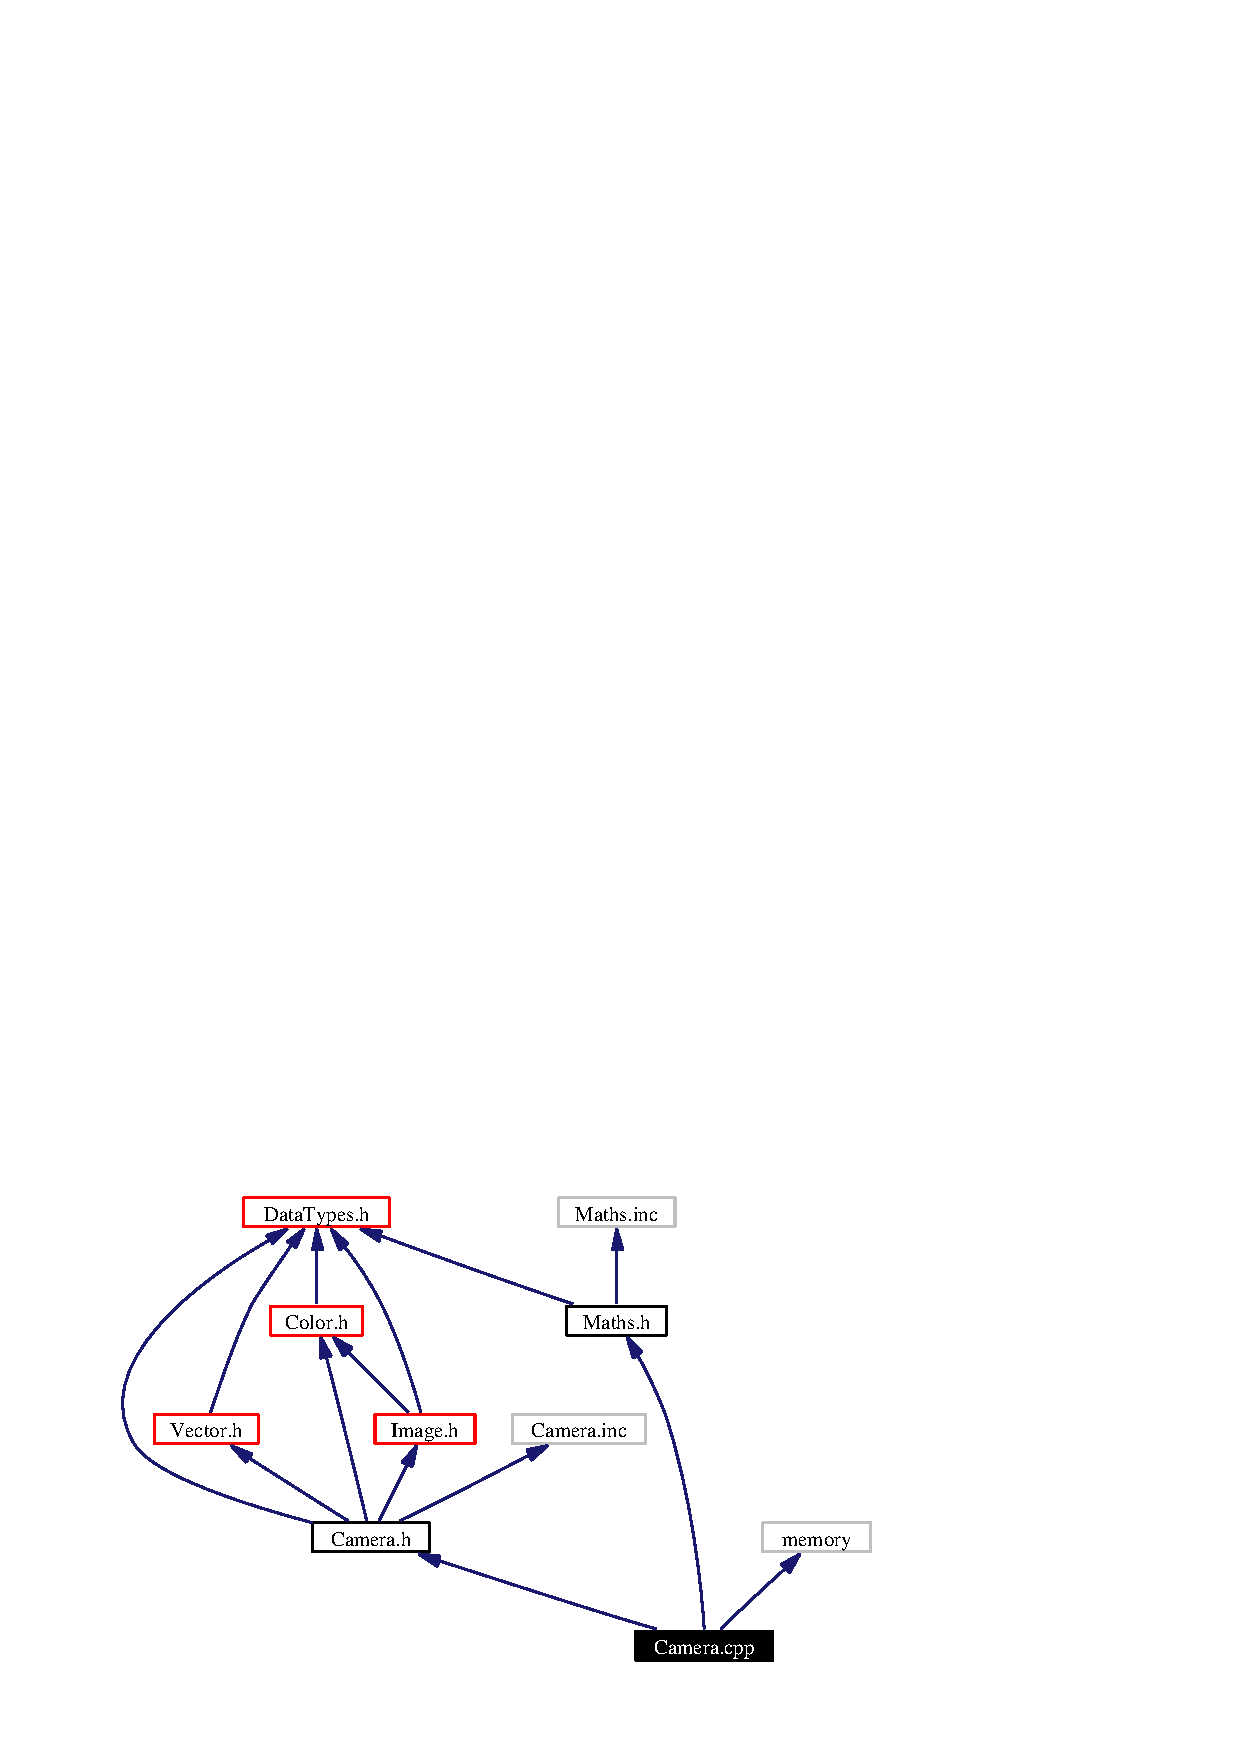
\includegraphics[width=209pt]{Camera_8cpp__incl}
\end{center}
\end{figure}

\section{Camera.h File Reference}
\label{Camera_8h}\index{Camera.h@{Camera.h}}
{\tt \#include \char`\"{}Data\-Types.h\char`\"{}}\par
{\tt \#include \char`\"{}Vector.h\char`\"{}}\par
{\tt \#include \char`\"{}Color.h\char`\"{}}\par
{\tt \#include \char`\"{}Image.h\char`\"{}}\par
{\tt \#include \char`\"{}Camera.inc\char`\"{}}\par


Include dependency graph for Camera.h:\begin{figure}[H]
\begin{center}
\leavevmode
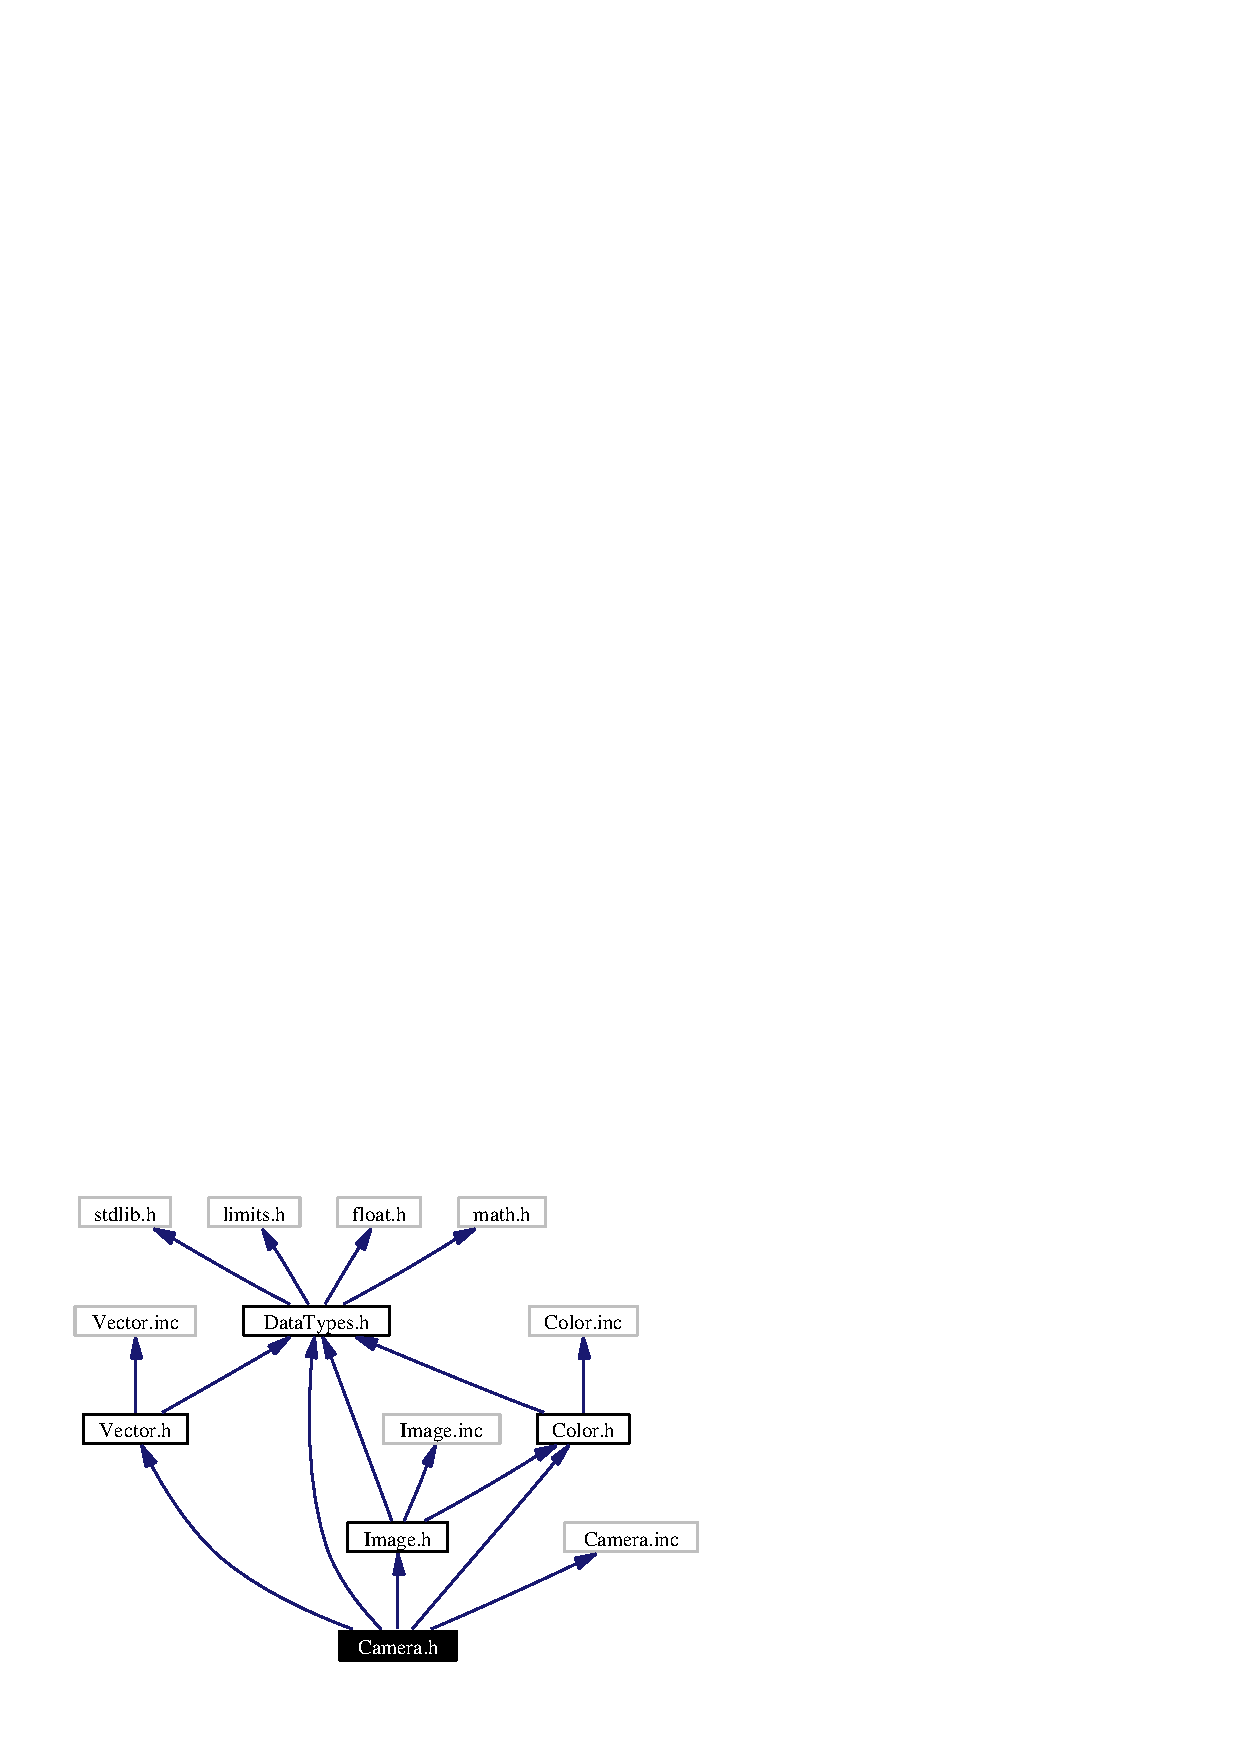
\includegraphics[width=168pt]{Camera_8h__incl}
\end{center}
\end{figure}


This graph shows which files directly or indirectly include this file:\begin{figure}[H]
\begin{center}
\leavevmode
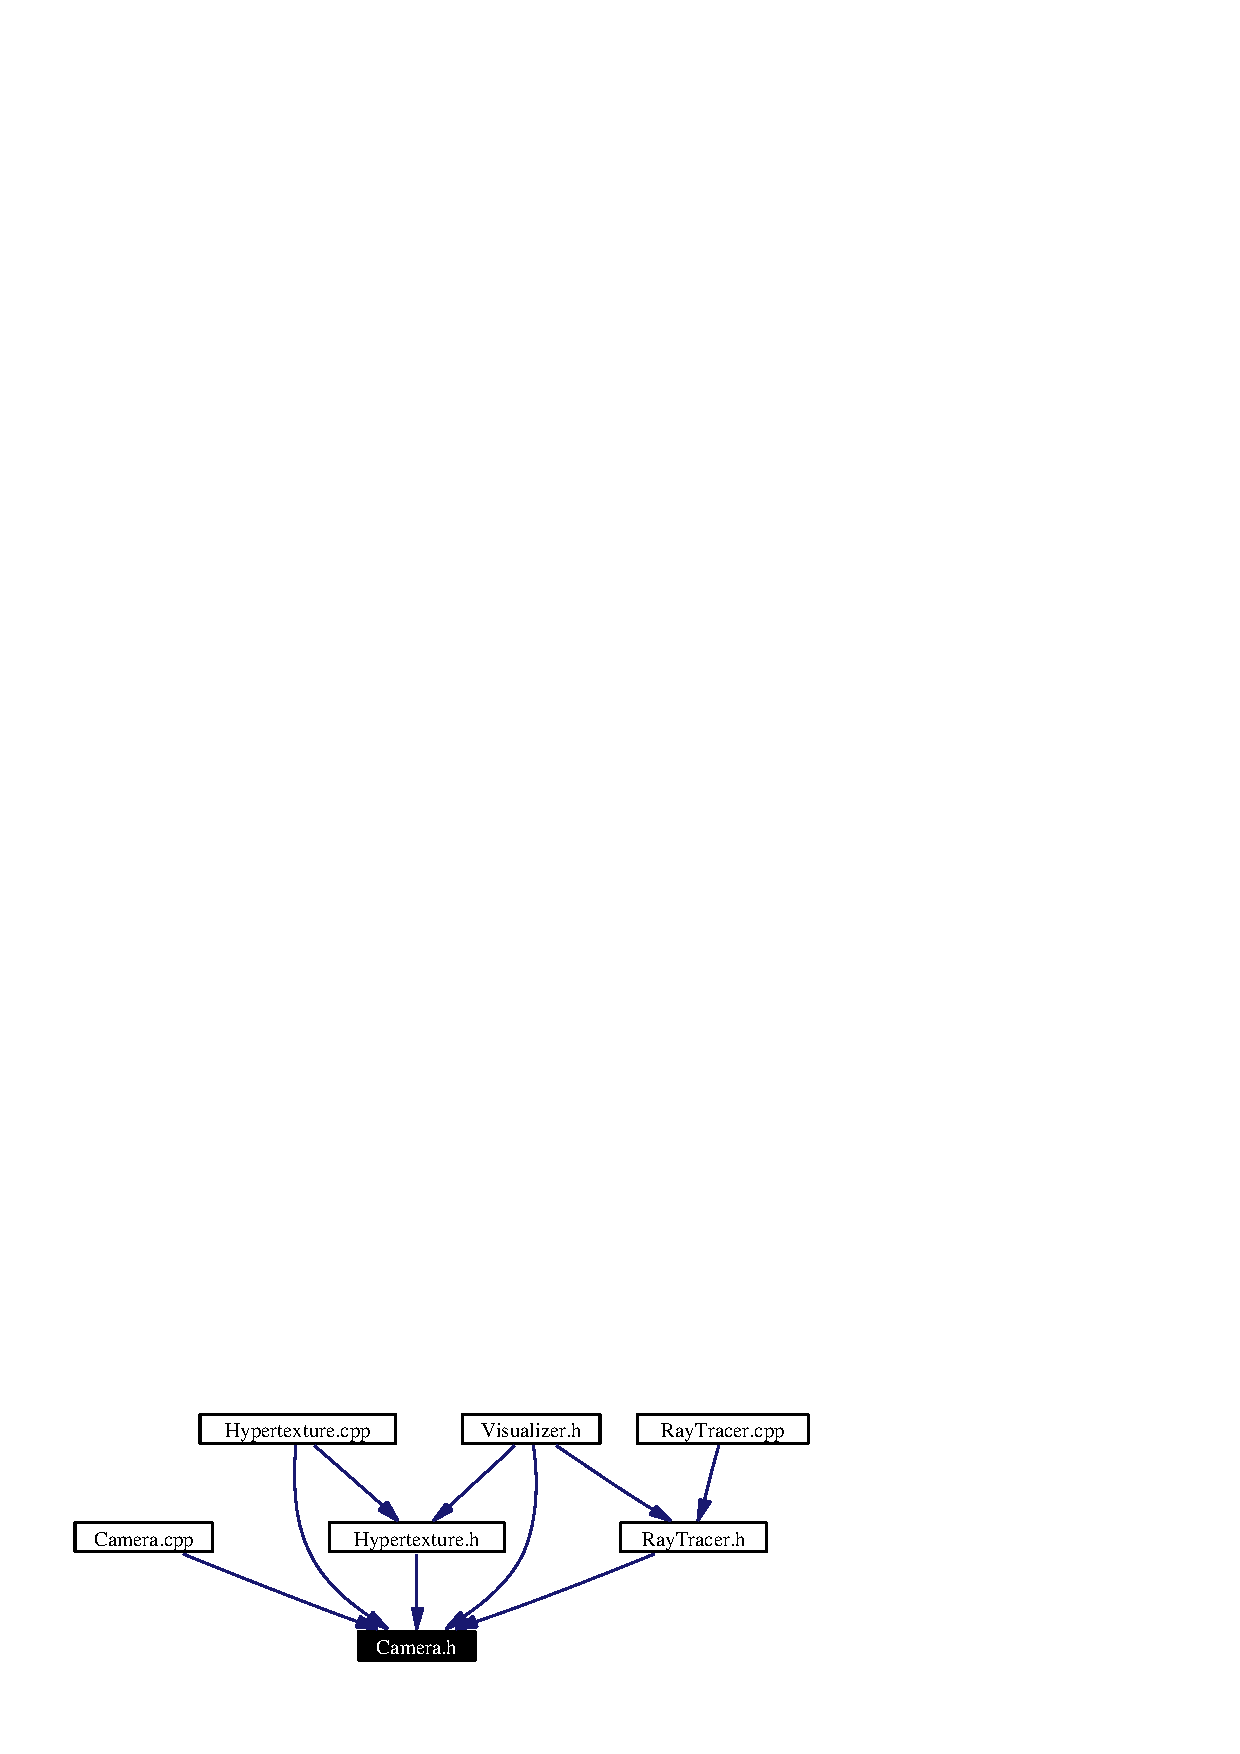
\includegraphics[width=194pt]{Camera_8h__dep__incl}
\end{center}
\end{figure}
\subsection*{Namespaces}
\begin{CompactItemize}
\item 
namespace {\bf dg}
\end{CompactItemize}

\section{Color.cpp File Reference}
\label{Color_8cpp}\index{Color.cpp@{Color.cpp}}
{\tt \#include \char`\"{}Color.h\char`\"{}}\par


Include dependency graph for Color.cpp:\begin{figure}[H]
\begin{center}
\leavevmode
\includegraphics[width=88pt]{Color_8cpp__incl}
\end{center}
\end{figure}

\section{Color.h File Reference}
\label{Color_8h}\index{Color.h@{Color.h}}
{\tt \#include \char`\"{}Data\-Types.h\char`\"{}}\par
{\tt \#include \char`\"{}Color.inc\char`\"{}}\par


Include dependency graph for Color.h:\begin{figure}[H]
\begin{center}
\leavevmode
\includegraphics[width=130pt]{Color_8h__incl}
\end{center}
\end{figure}


This graph shows which files directly or indirectly include this file:\begin{figure}[H]
\begin{center}
\leavevmode
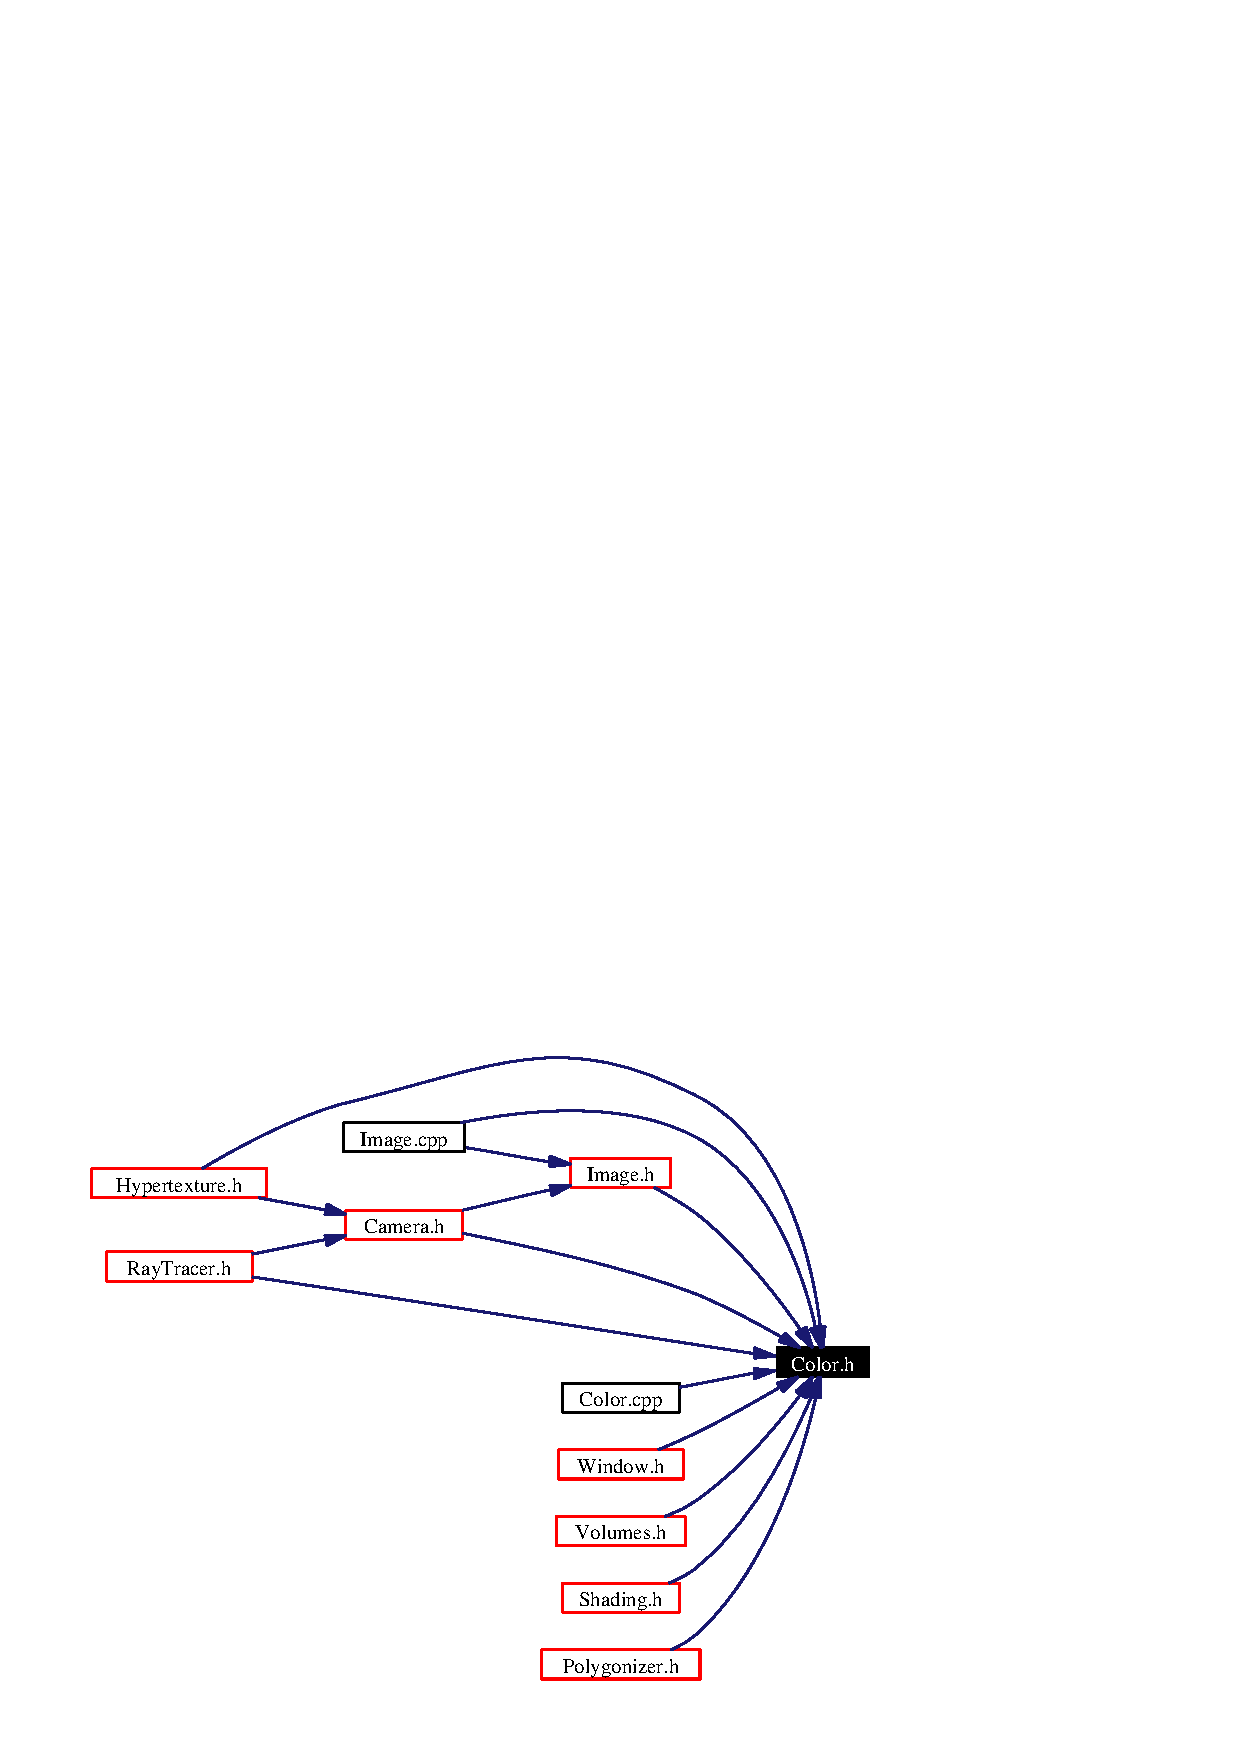
\includegraphics[width=213pt]{Color_8h__dep__incl}
\end{center}
\end{figure}
\subsection*{Namespaces}
\begin{CompactItemize}
\item 
namespace {\bf dg}
\end{CompactItemize}

\section{Cube\-Tables.h File Reference}
\label{CubeTables_8h}\index{CubeTables.h@{CubeTables.h}}


This graph shows which files directly or indirectly include this file:\begin{figure}[H]
\begin{center}
\leavevmode
\includegraphics[width=103pt]{CubeTables_8h__dep__incl}
\end{center}
\end{figure}
\subsection*{Namespaces}
\begin{CompactItemize}
\item 
namespace {\bf dg}
\end{CompactItemize}

\section{Data\-Types.h File Reference}
\label{DataTypes_8h}\index{DataTypes.h@{DataTypes.h}}
{\tt \#include $<$stdlib.h$>$}\par
{\tt \#include $<$limits.h$>$}\par
{\tt \#include $<$float.h$>$}\par
{\tt \#include $<$math.h$>$}\par


Include dependency graph for Data\-Types.h:\begin{figure}[H]
\begin{center}
\leavevmode
\includegraphics[width=130pt]{DataTypes_8h__incl}
\end{center}
\end{figure}


This graph shows which files directly or indirectly include this file:\begin{figure}[H]
\begin{center}
\leavevmode
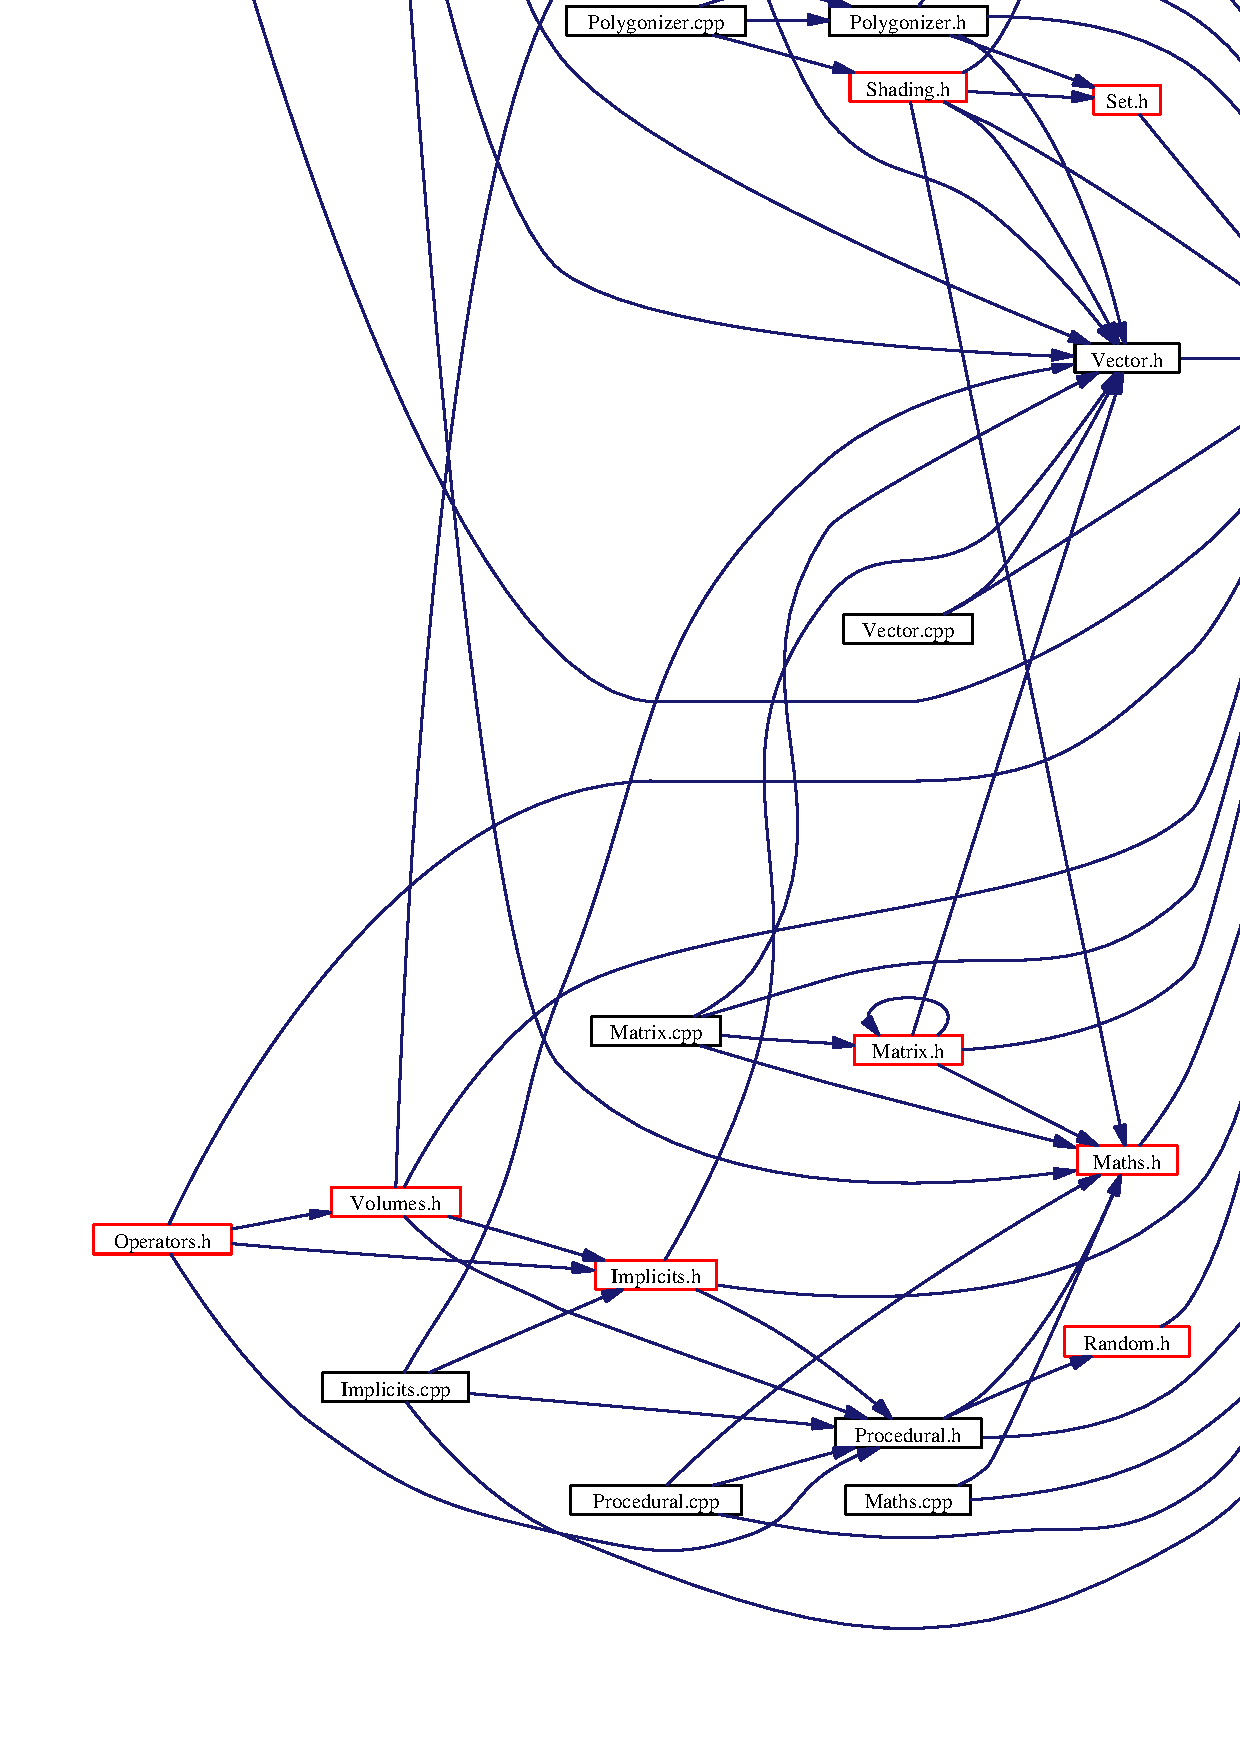
\includegraphics[width=344pt]{DataTypes_8h__dep__incl}
\end{center}
\end{figure}
\subsection*{Namespaces}
\begin{CompactItemize}
\item 
namespace {\bf dg}
\end{CompactItemize}

\section{Glut\-Headers.h File Reference}
\label{GlutHeaders_8h}\index{GlutHeaders.h@{GlutHeaders.h}}
{\tt \#include \char`\"{}Open\-GLHeaders.h\char`\"{}}\par
{\tt \#include $<$GL/glut.h$>$}\par


Include dependency graph for Glut\-Headers.h:\begin{figure}[H]
\begin{center}
\leavevmode
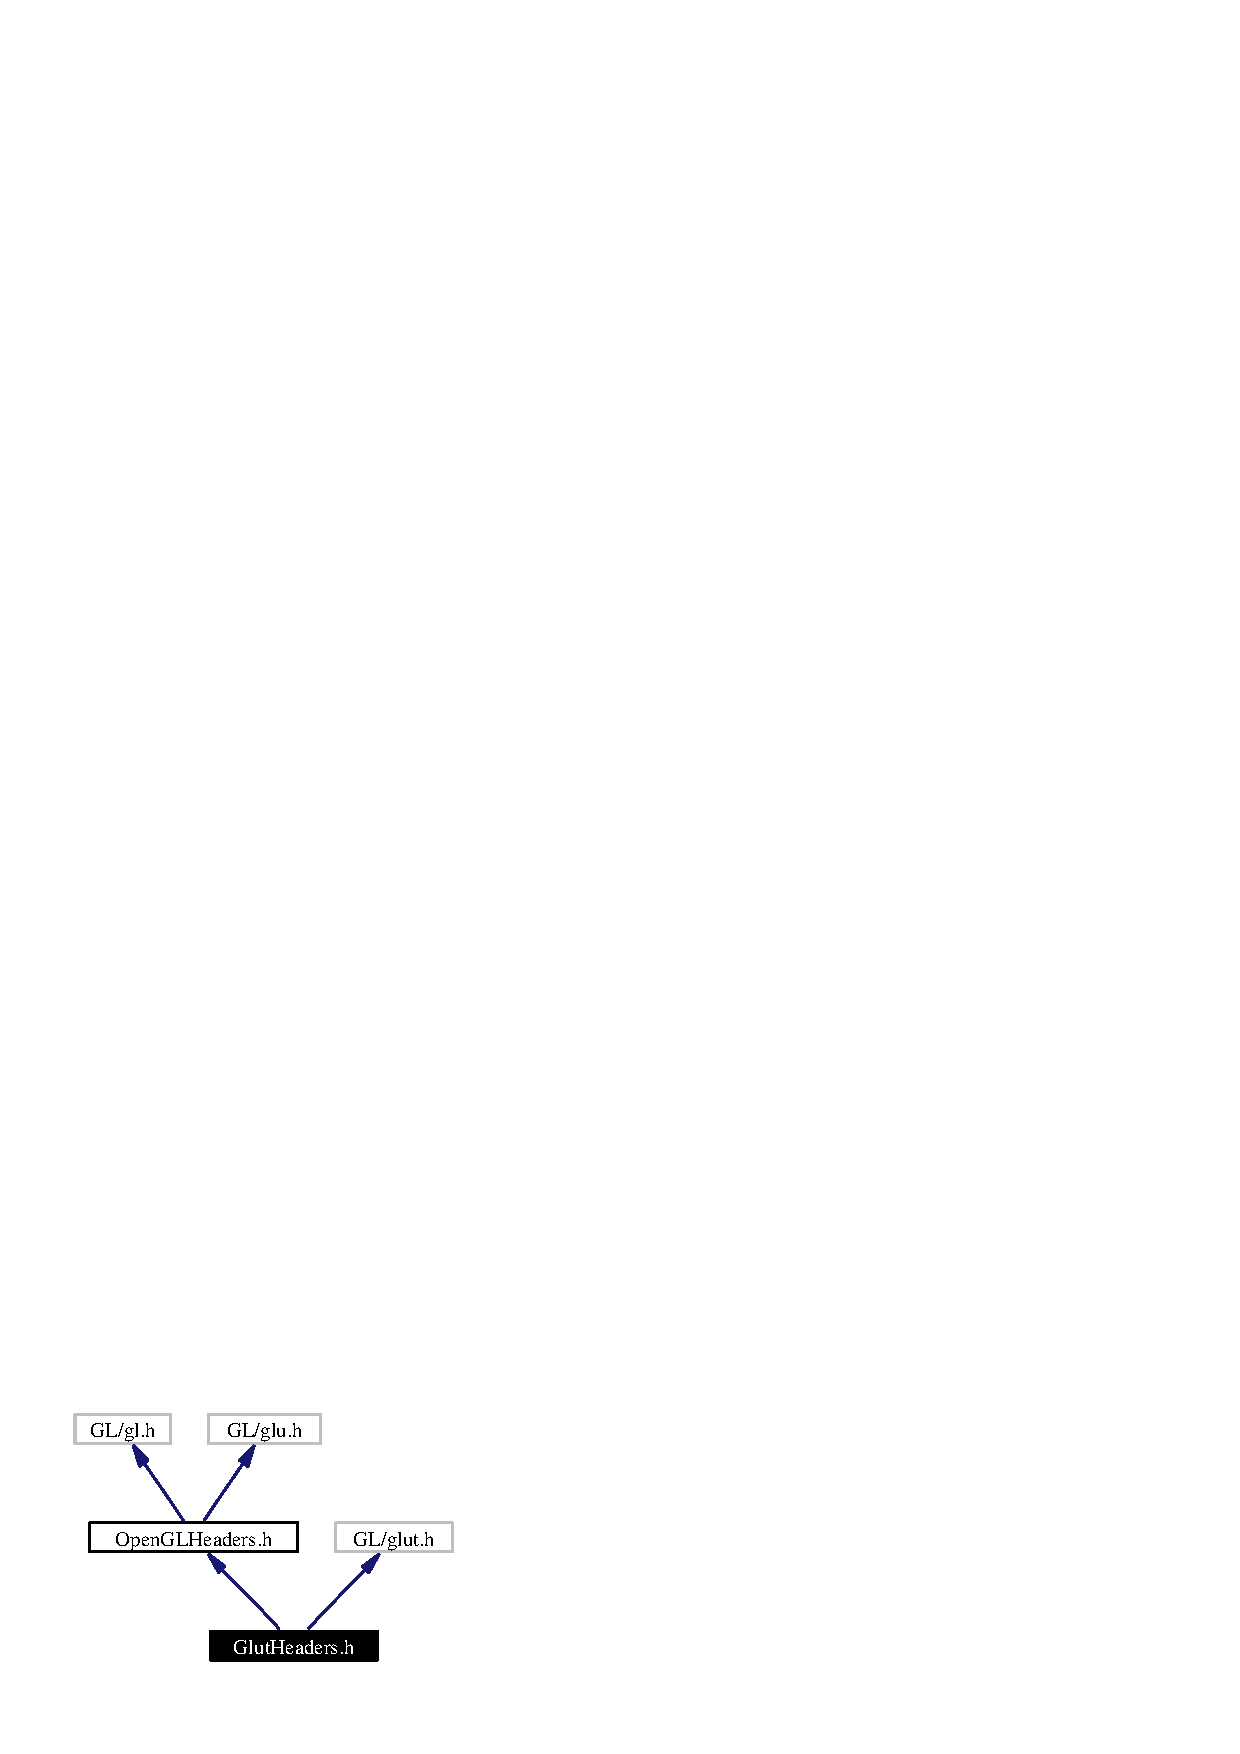
\includegraphics[width=109pt]{GlutHeaders_8h__incl}
\end{center}
\end{figure}


This graph shows which files directly or indirectly include this file:\begin{figure}[H]
\begin{center}
\leavevmode
\includegraphics[width=137pt]{GlutHeaders_8h__dep__incl}
\end{center}
\end{figure}

\section{Glut\-Key\-Bindings.h File Reference}
\label{GlutKeyBindings_8h}\index{GlutKeyBindings.h@{GlutKeyBindings.h}}
{\tt \#include \char`\"{}Glut\-Headers.h\char`\"{}}\par


Include dependency graph for Glut\-Key\-Bindings.h:\begin{figure}[H]
\begin{center}
\leavevmode
\includegraphics[width=105pt]{GlutKeyBindings_8h__incl}
\end{center}
\end{figure}


This graph shows which files directly or indirectly include this file:\begin{figure}[H]
\begin{center}
\leavevmode
\includegraphics[width=70pt]{GlutKeyBindings_8h__dep__incl}
\end{center}
\end{figure}

\section{Glut\-Window.cpp File Reference}
\label{GlutWindow_8cpp}\index{GlutWindow.cpp@{GlutWindow.cpp}}
{\tt \#include \char`\"{}Data\-Types.h\char`\"{}}\par
{\tt \#include \char`\"{}Window.h\char`\"{}}\par
{\tt \#include \char`\"{}Glut\-Key\-Bindings.h\char`\"{}}\par
{\tt \#include \char`\"{}Glut\-Headers.h\char`\"{}}\par


Include dependency graph for Glut\-Window.cpp:\begin{figure}[H]
\begin{center}
\leavevmode
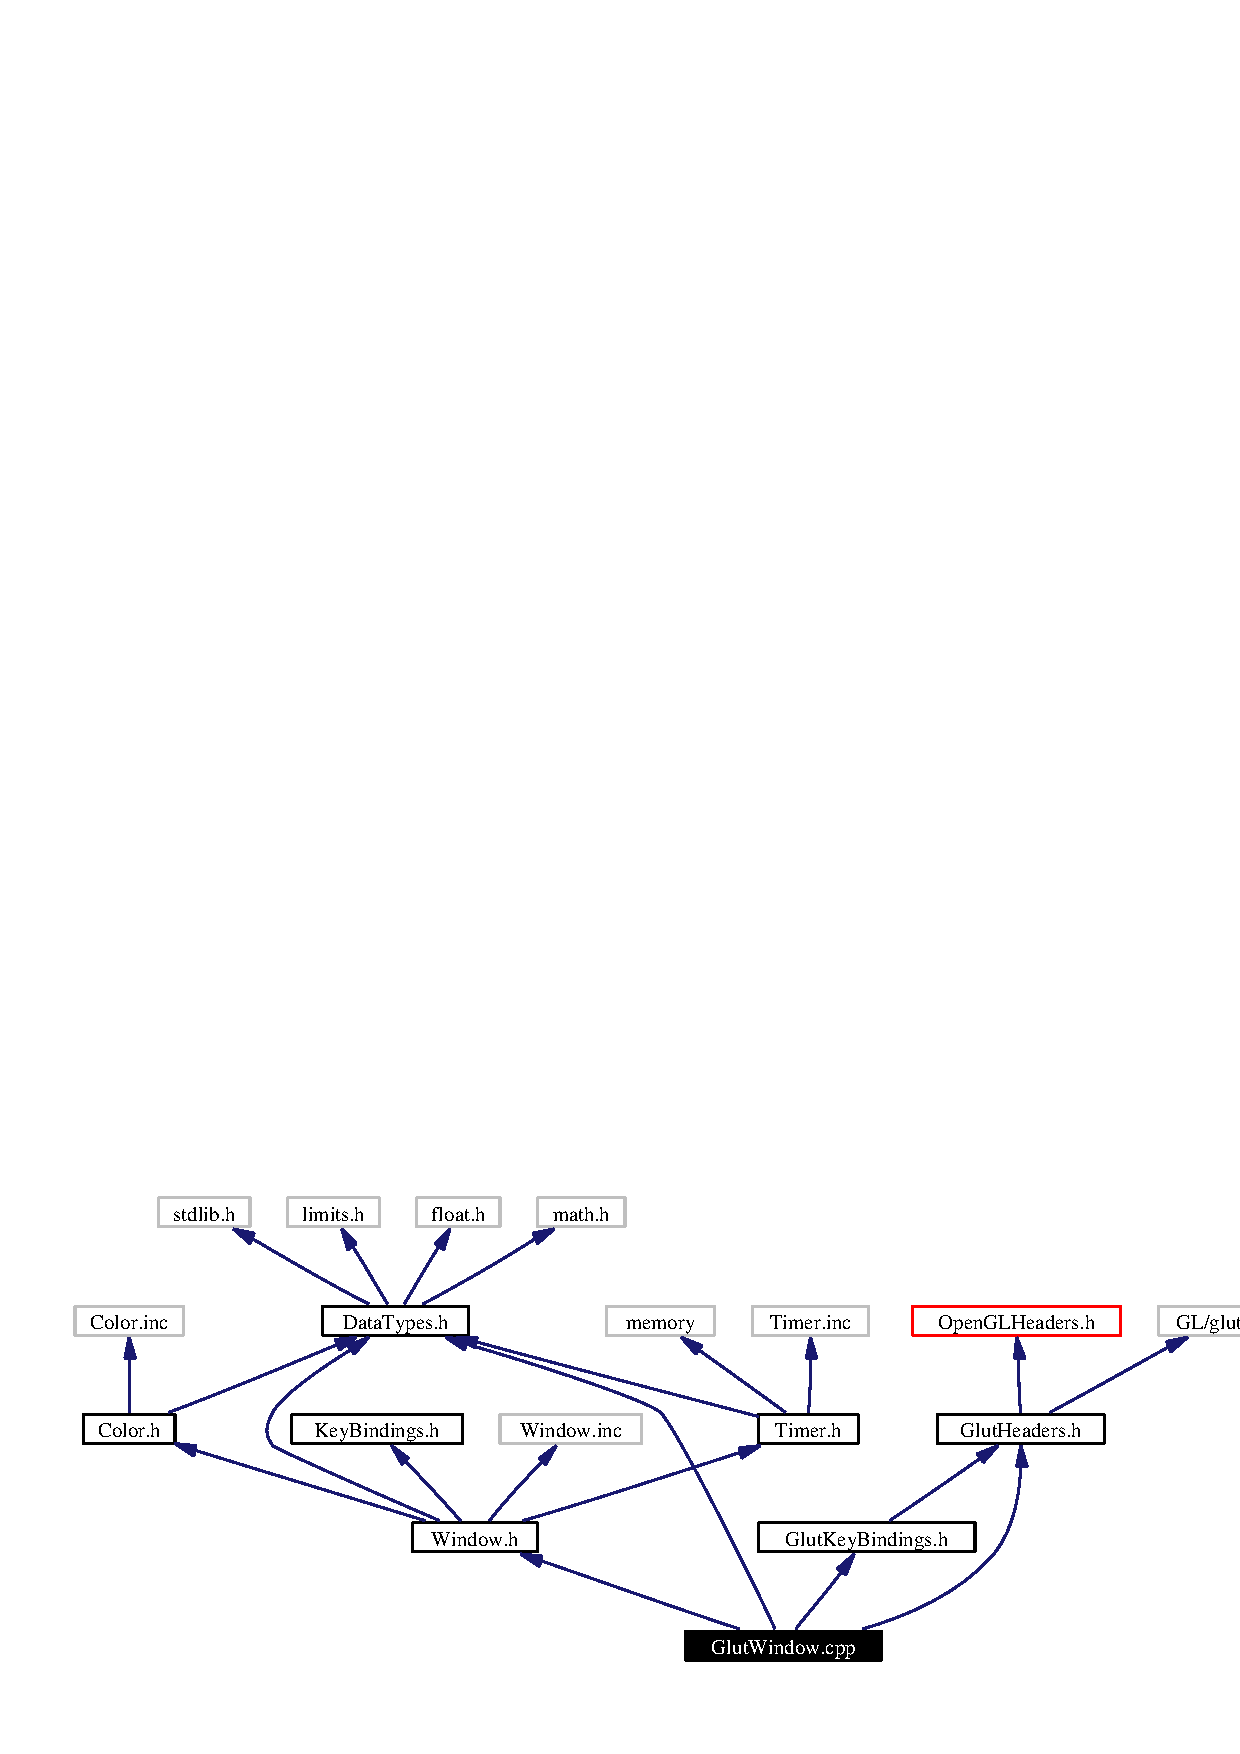
\includegraphics[width=306pt]{GlutWindow_8cpp__incl}
\end{center}
\end{figure}
\subsection*{Functions}
\begin{CompactItemize}
\item 
int {\bf main} (int argc, char $\ast$$\ast$argv)
\end{CompactItemize}


\subsection{Function Documentation}
\index{GlutWindow.cpp@{Glut\-Window.cpp}!main@{main}}
\index{main@{main}!GlutWindow.cpp@{Glut\-Window.cpp}}
\subsubsection{\setlength{\rightskip}{0pt plus 5cm}int main (int {\em argc}, char $\ast$$\ast$ {\em argv})}\label{GlutWindow_8cpp_a13}




Definition at line 271 of file Glut\-Window.cpp.
\section{Hypertexture.cpp File Reference}
\label{Hypertexture_8cpp}\index{Hypertexture.cpp@{Hypertexture.cpp}}
{\tt \#include \char`\"{}Hypertexture.h\char`\"{}}\par
{\tt \#include \char`\"{}Operators.h\char`\"{}}\par
{\tt \#include \char`\"{}Random.h\char`\"{}}\par
{\tt \#include \char`\"{}Camera.h\char`\"{}}\par
{\tt \#include \char`\"{}Image.h\char`\"{}}\par
{\tt \#include \char`\"{}Maths.h\char`\"{}}\par
{\tt \#include \char`\"{}Shading.h\char`\"{}}\par
{\tt \#include $<$memory$>$}\par


Include dependency graph for Hypertexture.cpp:\begin{figure}[H]
\begin{center}
\leavevmode
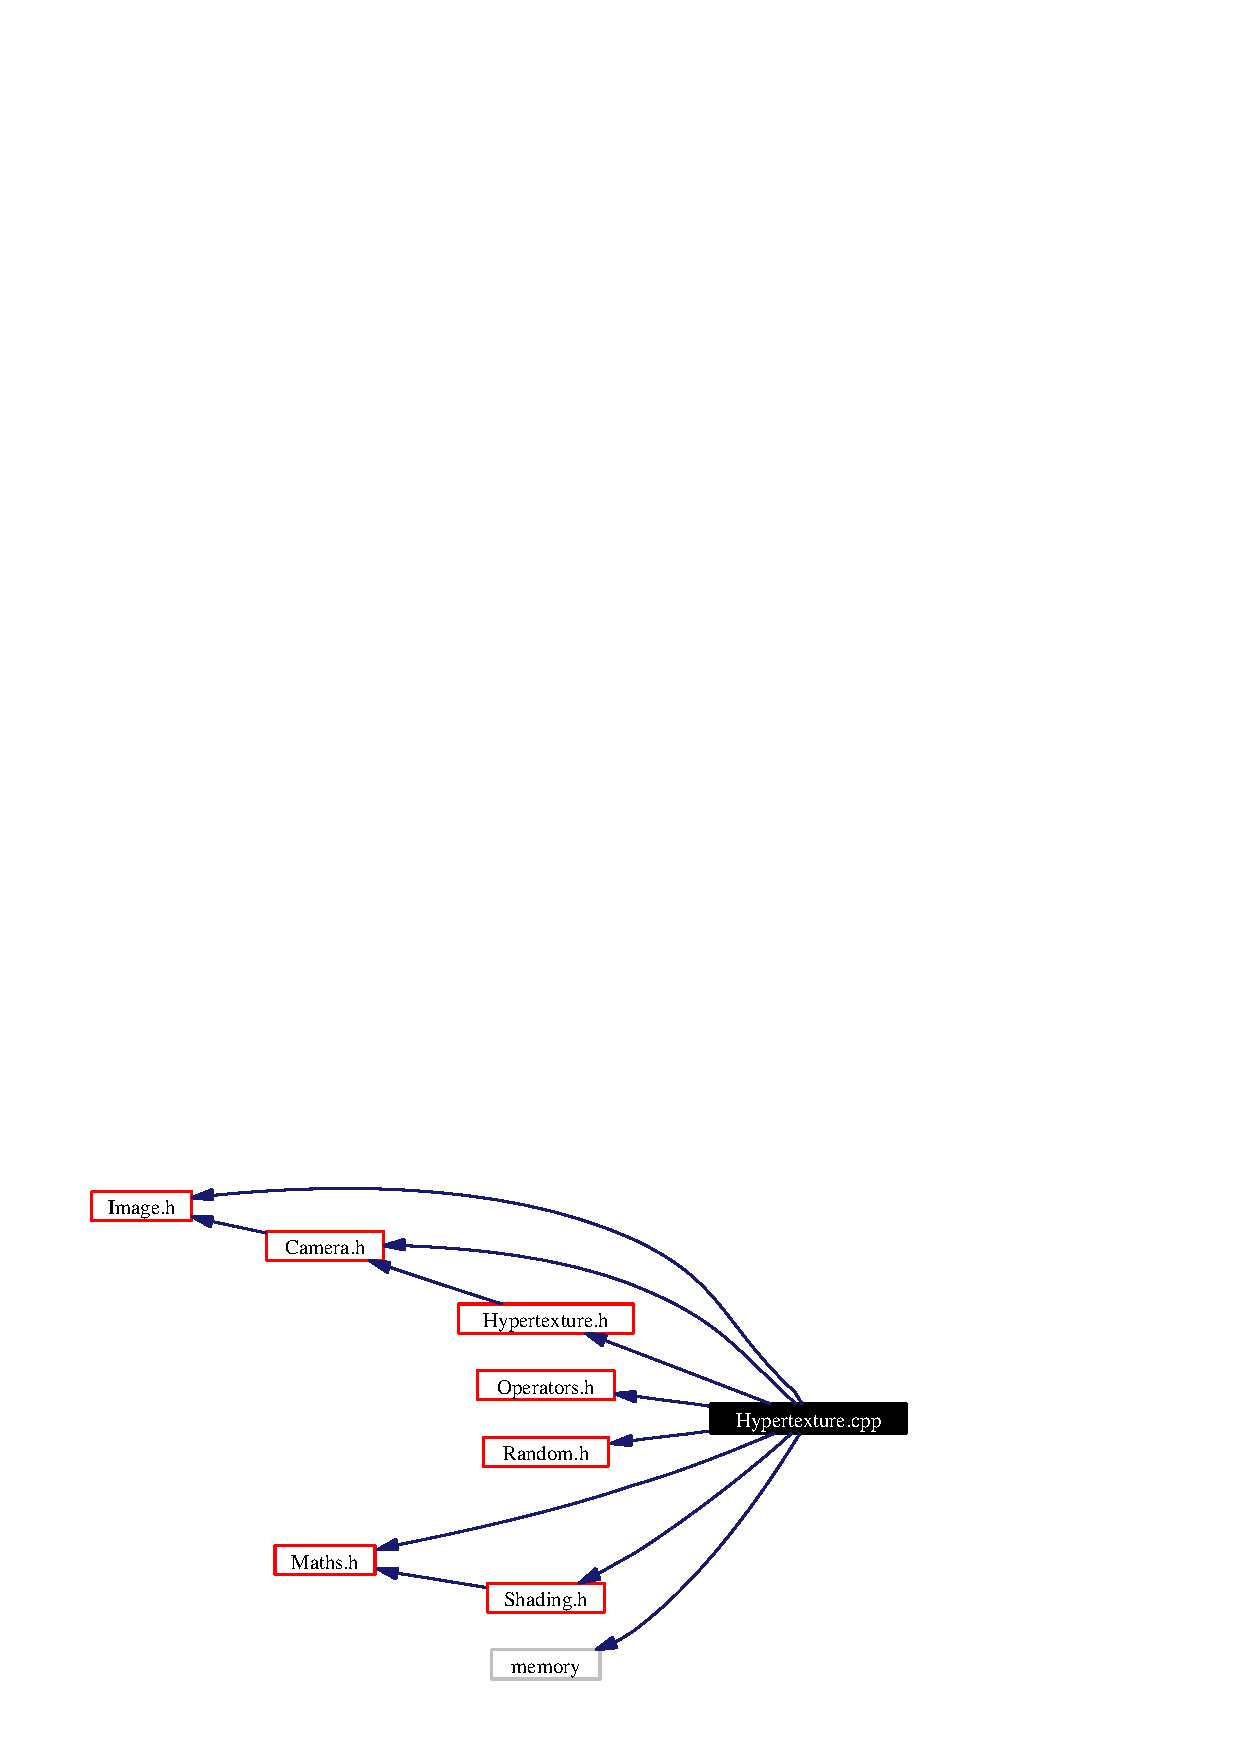
\includegraphics[width=222pt]{Hypertexture_8cpp__incl}
\end{center}
\end{figure}

\section{Hypertexture.h File Reference}
\label{Hypertexture_8h}\index{Hypertexture.h@{Hypertexture.h}}
{\tt \#include \char`\"{}Data\-Types.h\char`\"{}}\par
{\tt \#include \char`\"{}Camera.h\char`\"{}}\par
{\tt \#include \char`\"{}Vector.h\char`\"{}}\par
{\tt \#include \char`\"{}Color.h\char`\"{}}\par
{\tt \#include \char`\"{}Hypertexture.inc\char`\"{}}\par


Include dependency graph for Hypertexture.h:\begin{figure}[H]
\begin{center}
\leavevmode
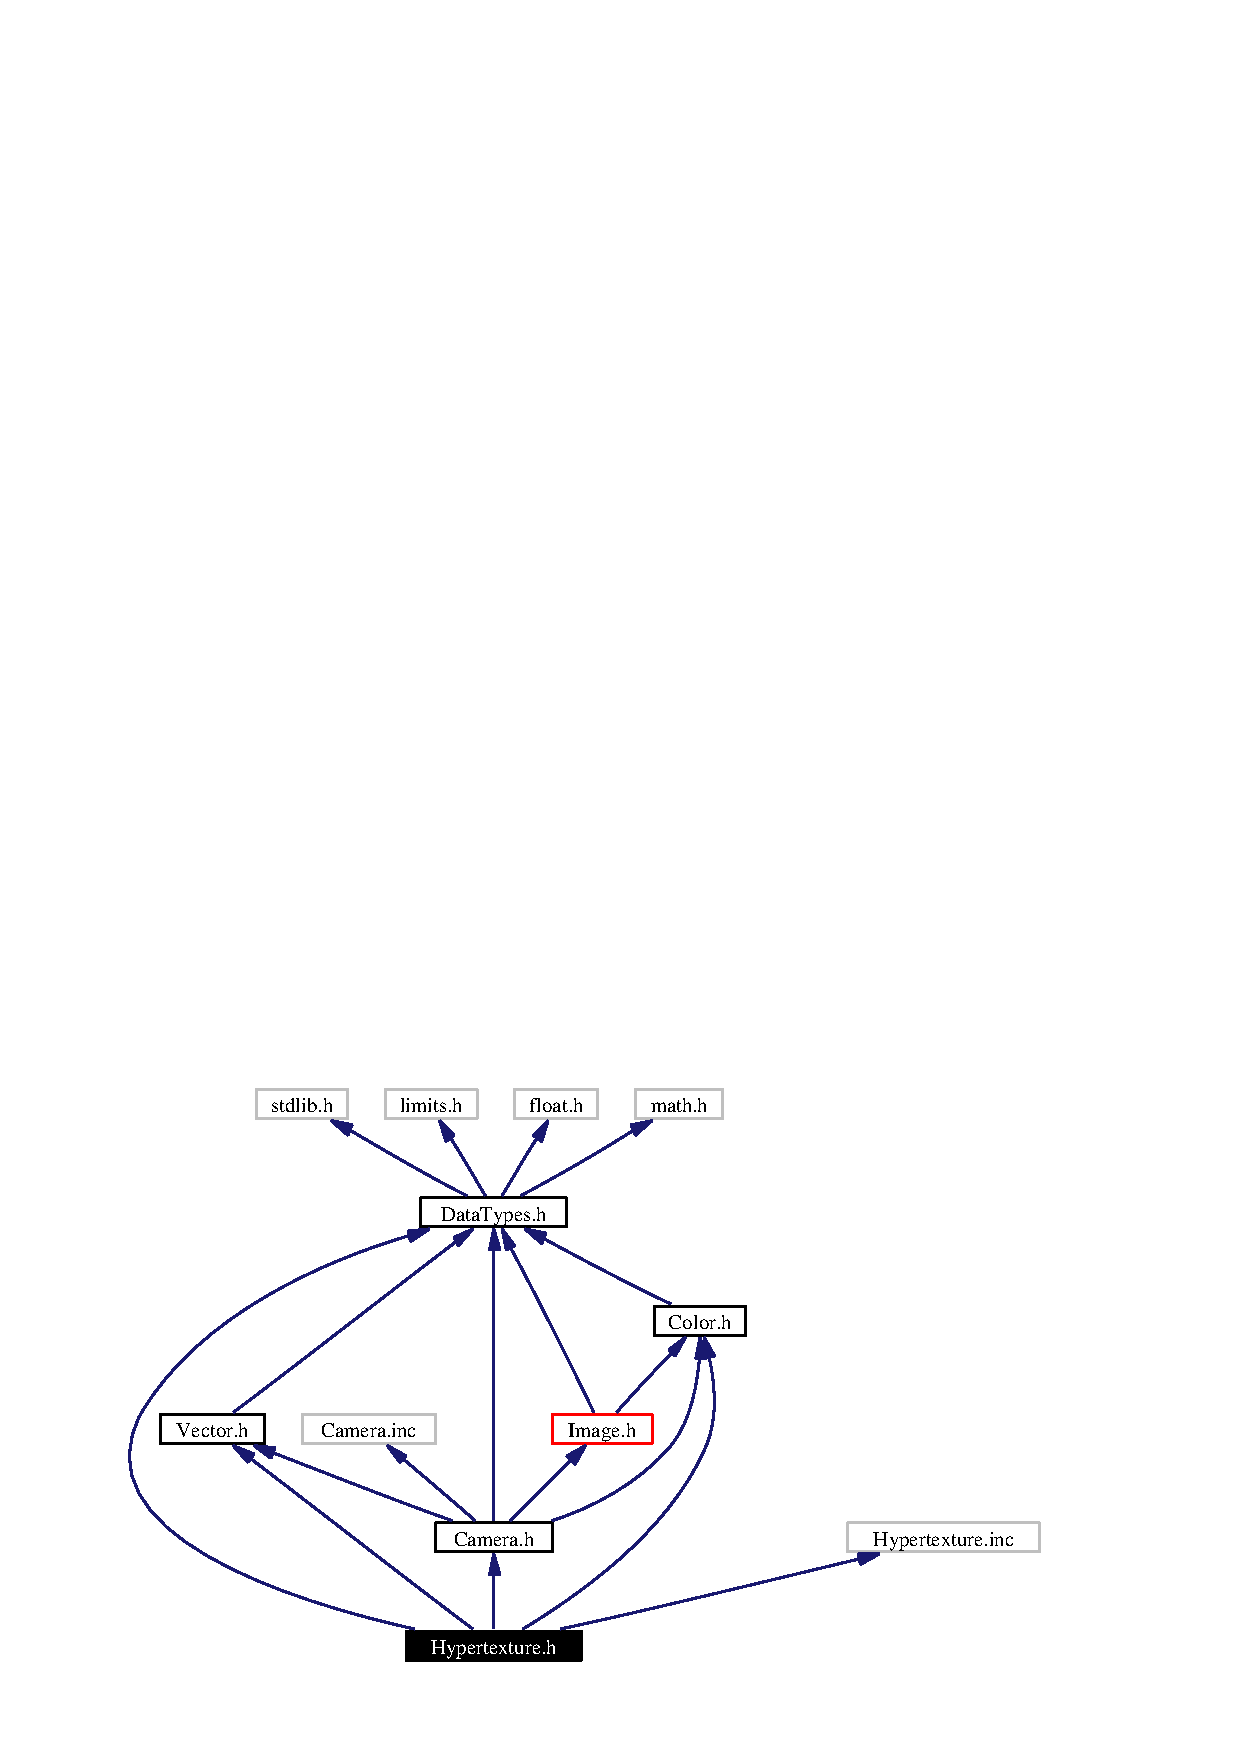
\includegraphics[width=250pt]{Hypertexture_8h__incl}
\end{center}
\end{figure}


This graph shows which files directly or indirectly include this file:\begin{figure}[H]
\begin{center}
\leavevmode
\includegraphics[width=110pt]{Hypertexture_8h__dep__incl}
\end{center}
\end{figure}
\subsection*{Namespaces}
\begin{CompactItemize}
\item 
namespace {\bf dg}
\end{CompactItemize}

\section{Image.cpp File Reference}
\label{Image_8cpp}\index{Image.cpp@{Image.cpp}}
{\tt \#include \char`\"{}Data\-Types.h\char`\"{}}\par
{\tt \#include \char`\"{}Image.h\char`\"{}}\par
{\tt \#include \char`\"{}Color.h\char`\"{}}\par
{\tt \#include $<$memory$>$}\par


Include dependency graph for Image.cpp:\begin{figure}[H]
\begin{center}
\leavevmode
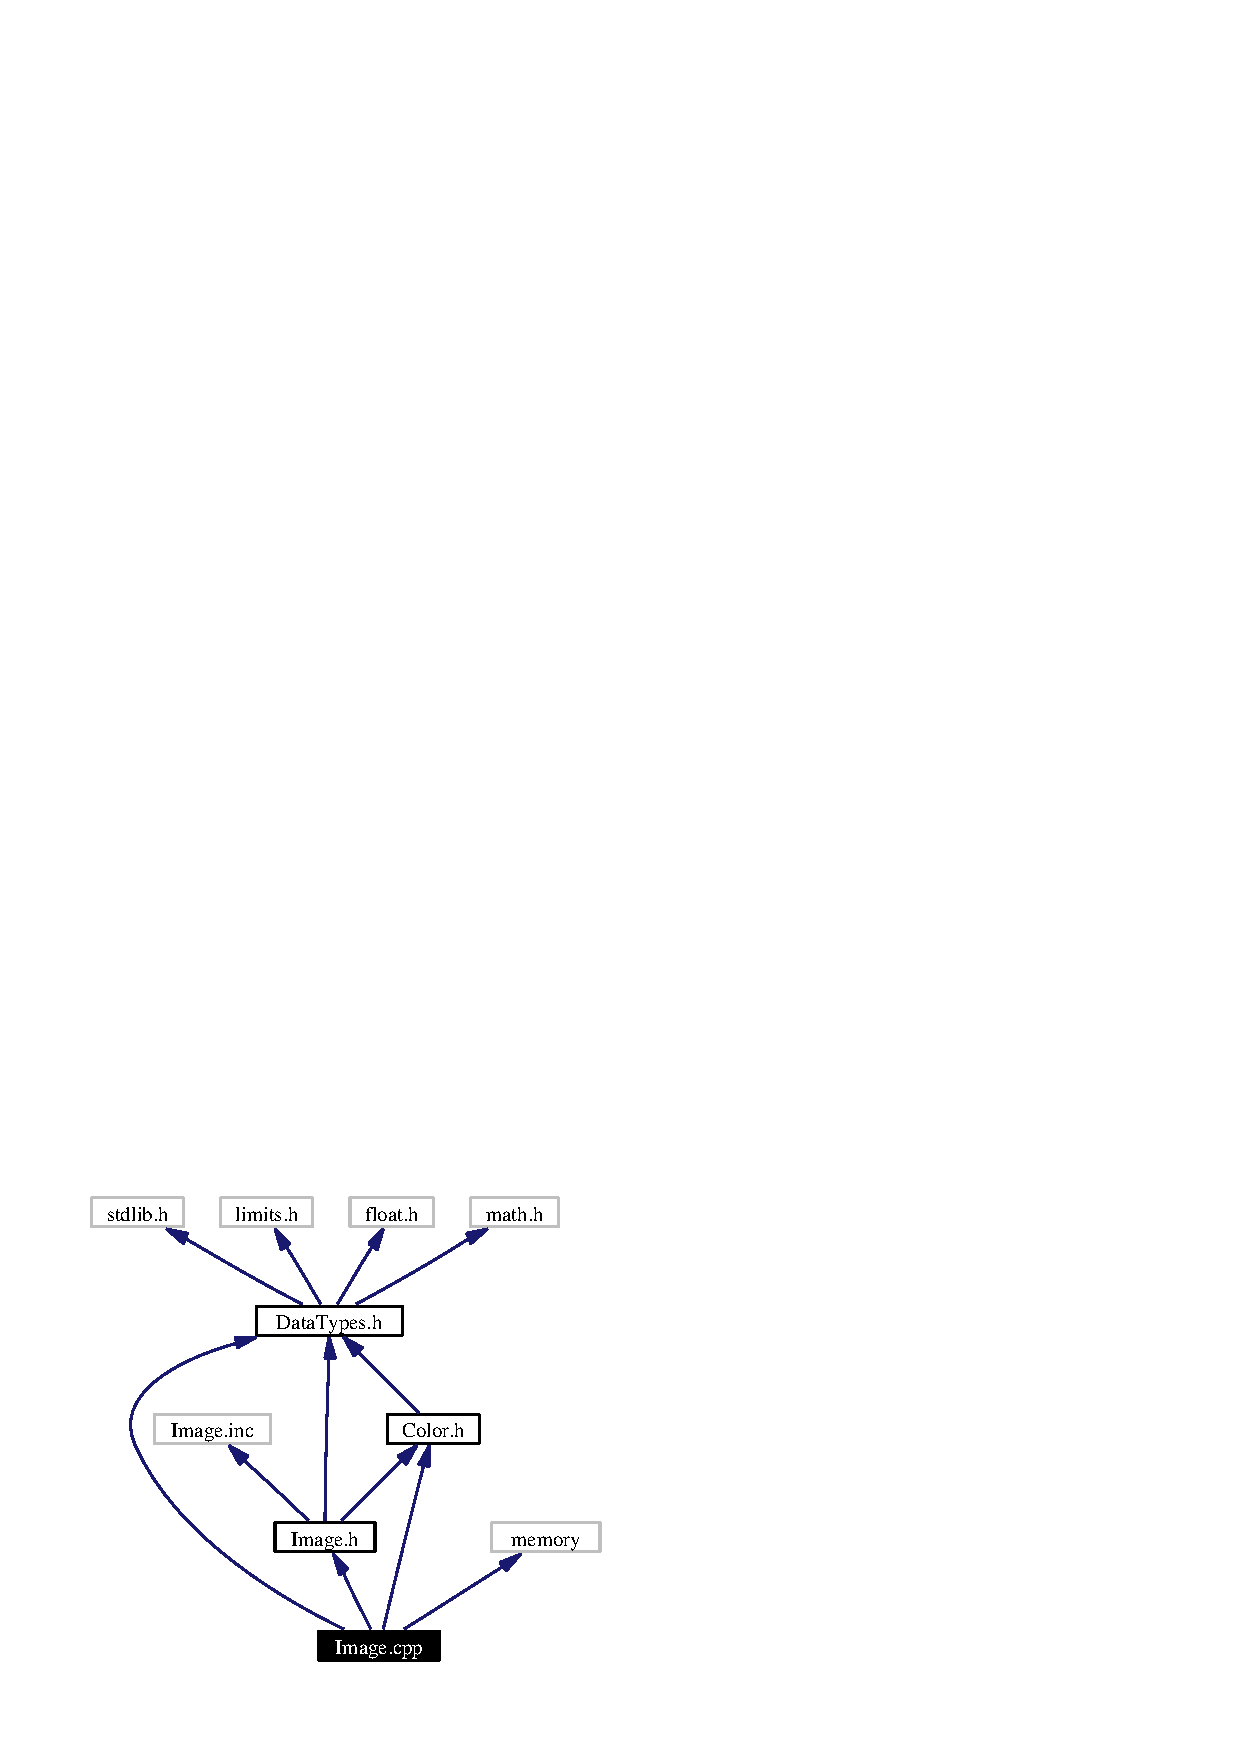
\includegraphics[width=144pt]{Image_8cpp__incl}
\end{center}
\end{figure}

\section{Image.h File Reference}
\label{Image_8h}\index{Image.h@{Image.h}}
{\tt \#include \char`\"{}Data\-Types.h\char`\"{}}\par
{\tt \#include \char`\"{}Color.h\char`\"{}}\par
{\tt \#include \char`\"{}Image.inc\char`\"{}}\par


Include dependency graph for Image.h:\begin{figure}[H]
\begin{center}
\leavevmode
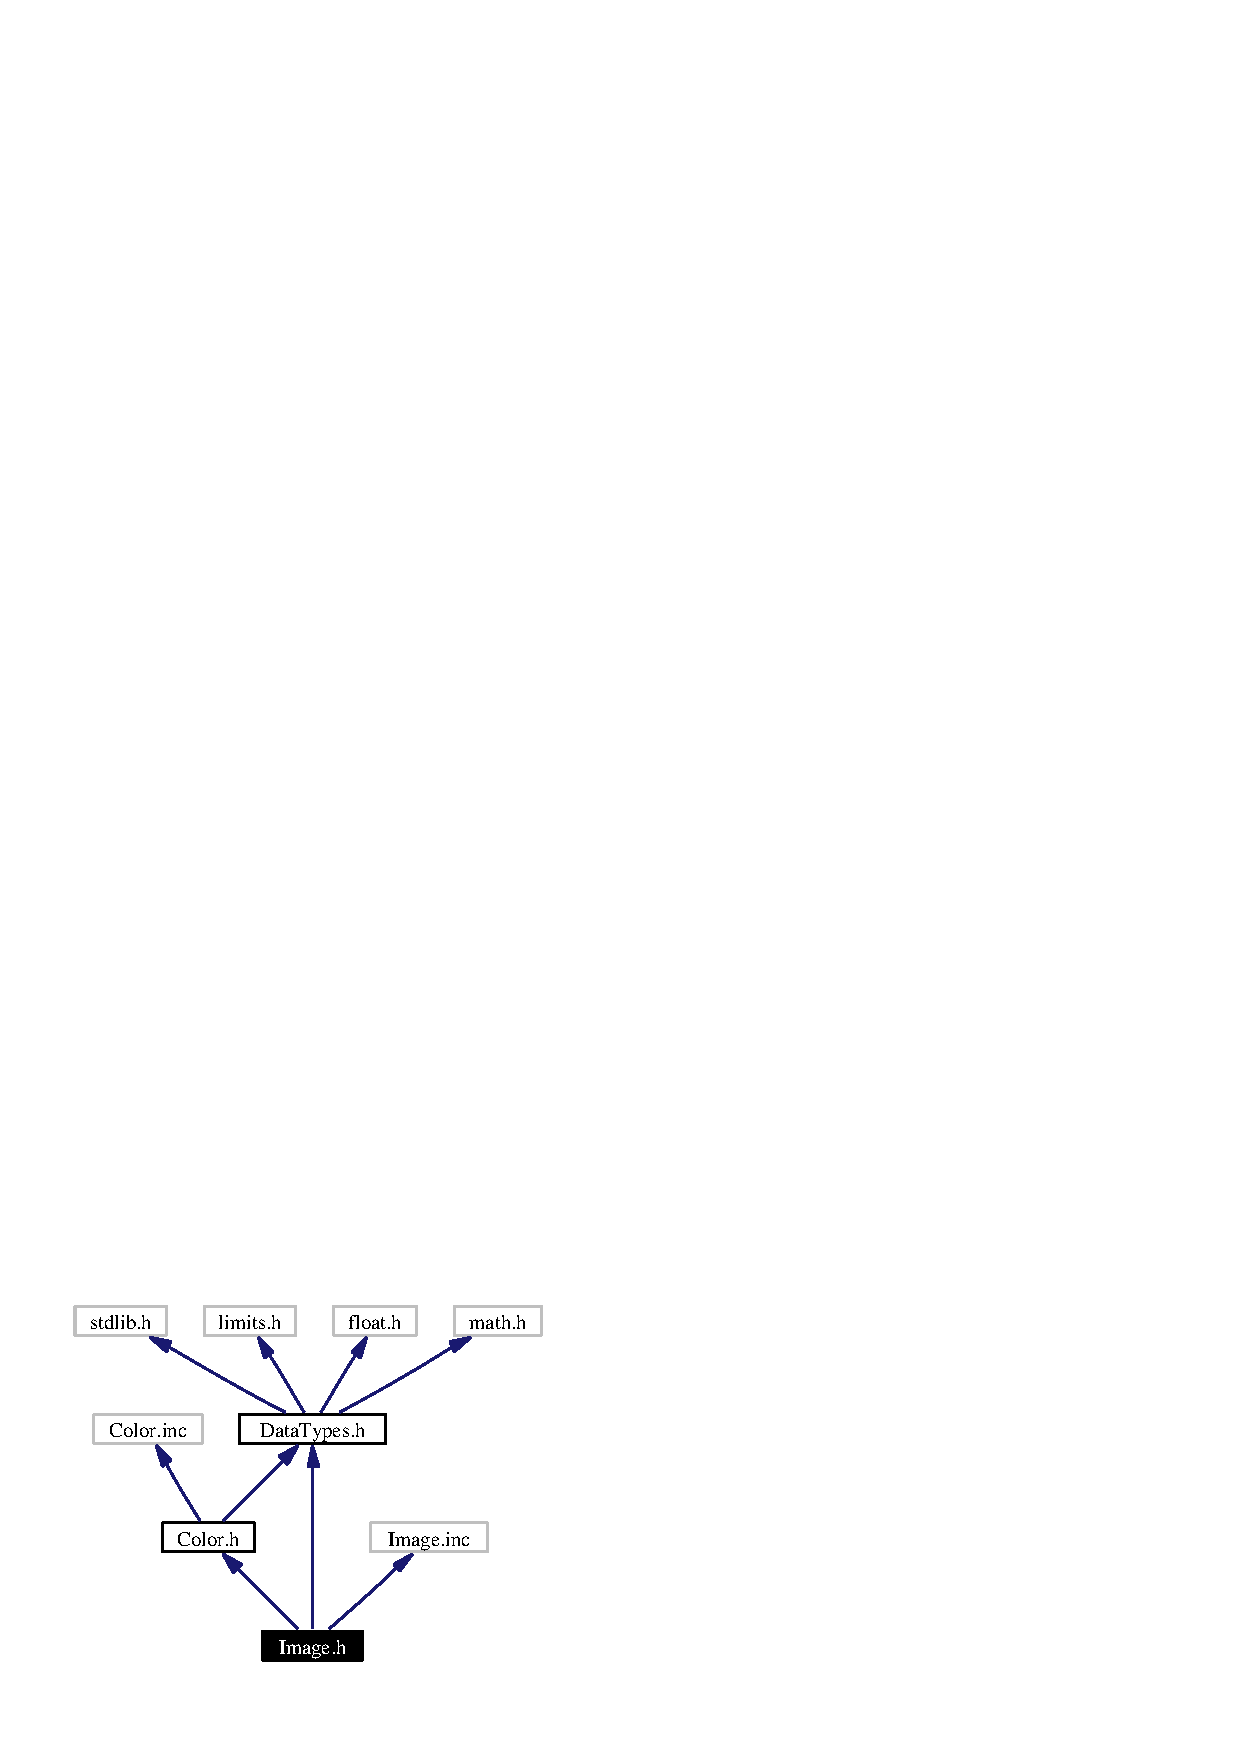
\includegraphics[width=130pt]{Image_8h__incl}
\end{center}
\end{figure}


This graph shows which files directly or indirectly include this file:\begin{figure}[H]
\begin{center}
\leavevmode
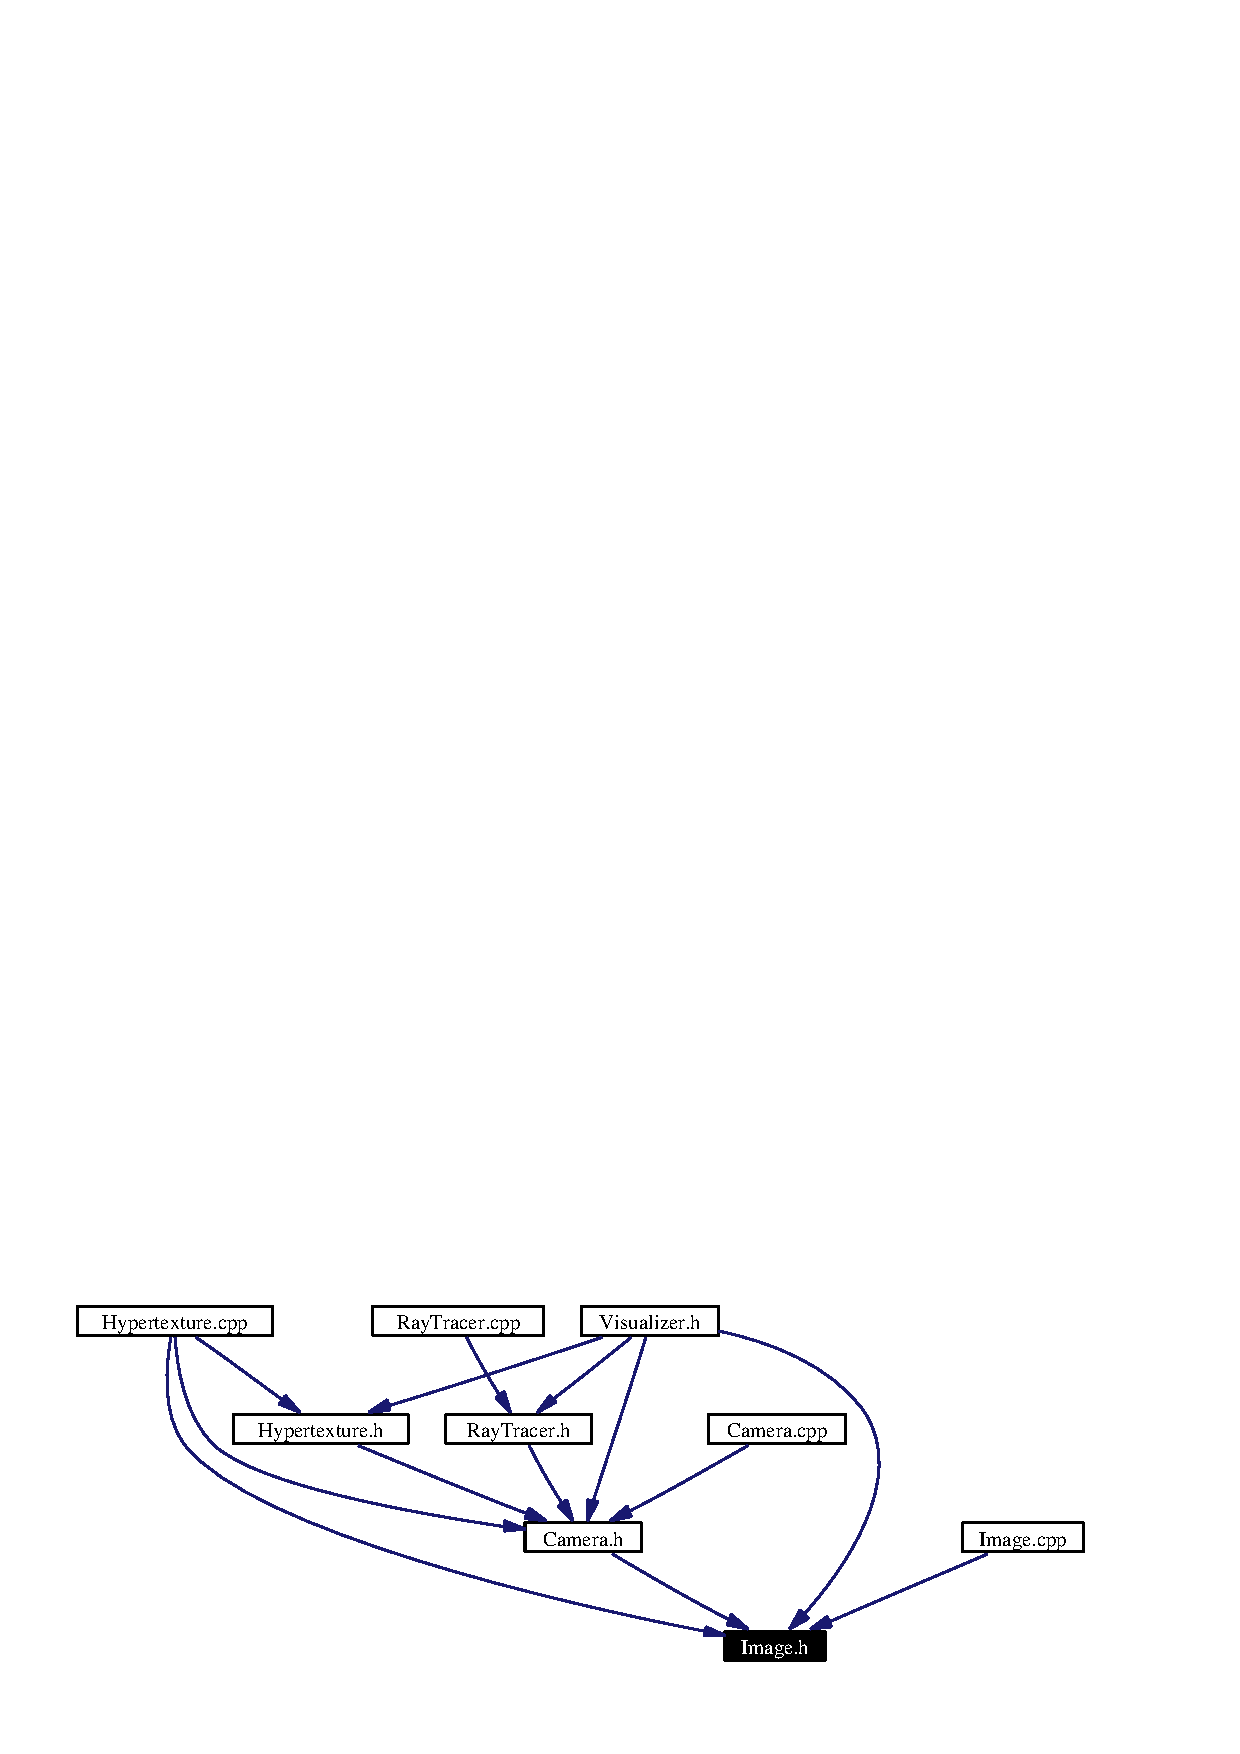
\includegraphics[width=260pt]{Image_8h__dep__incl}
\end{center}
\end{figure}
\subsection*{Namespaces}
\begin{CompactItemize}
\item 
namespace {\bf dg}
\end{CompactItemize}

\section{Implicits.cpp File Reference}
\label{Implicits_8cpp}\index{Implicits.cpp@{Implicits.cpp}}
{\tt \#include \char`\"{}Implicits.h\char`\"{}}\par
{\tt \#include \char`\"{}Data\-Types.h\char`\"{}}\par
{\tt \#include \char`\"{}Vector.h\char`\"{}}\par
{\tt \#include \char`\"{}Procedural.h\char`\"{}}\par
{\tt \#include $<$cstdio$>$}\par


Include dependency graph for Implicits.cpp:\begin{figure}[H]
\begin{center}
\leavevmode
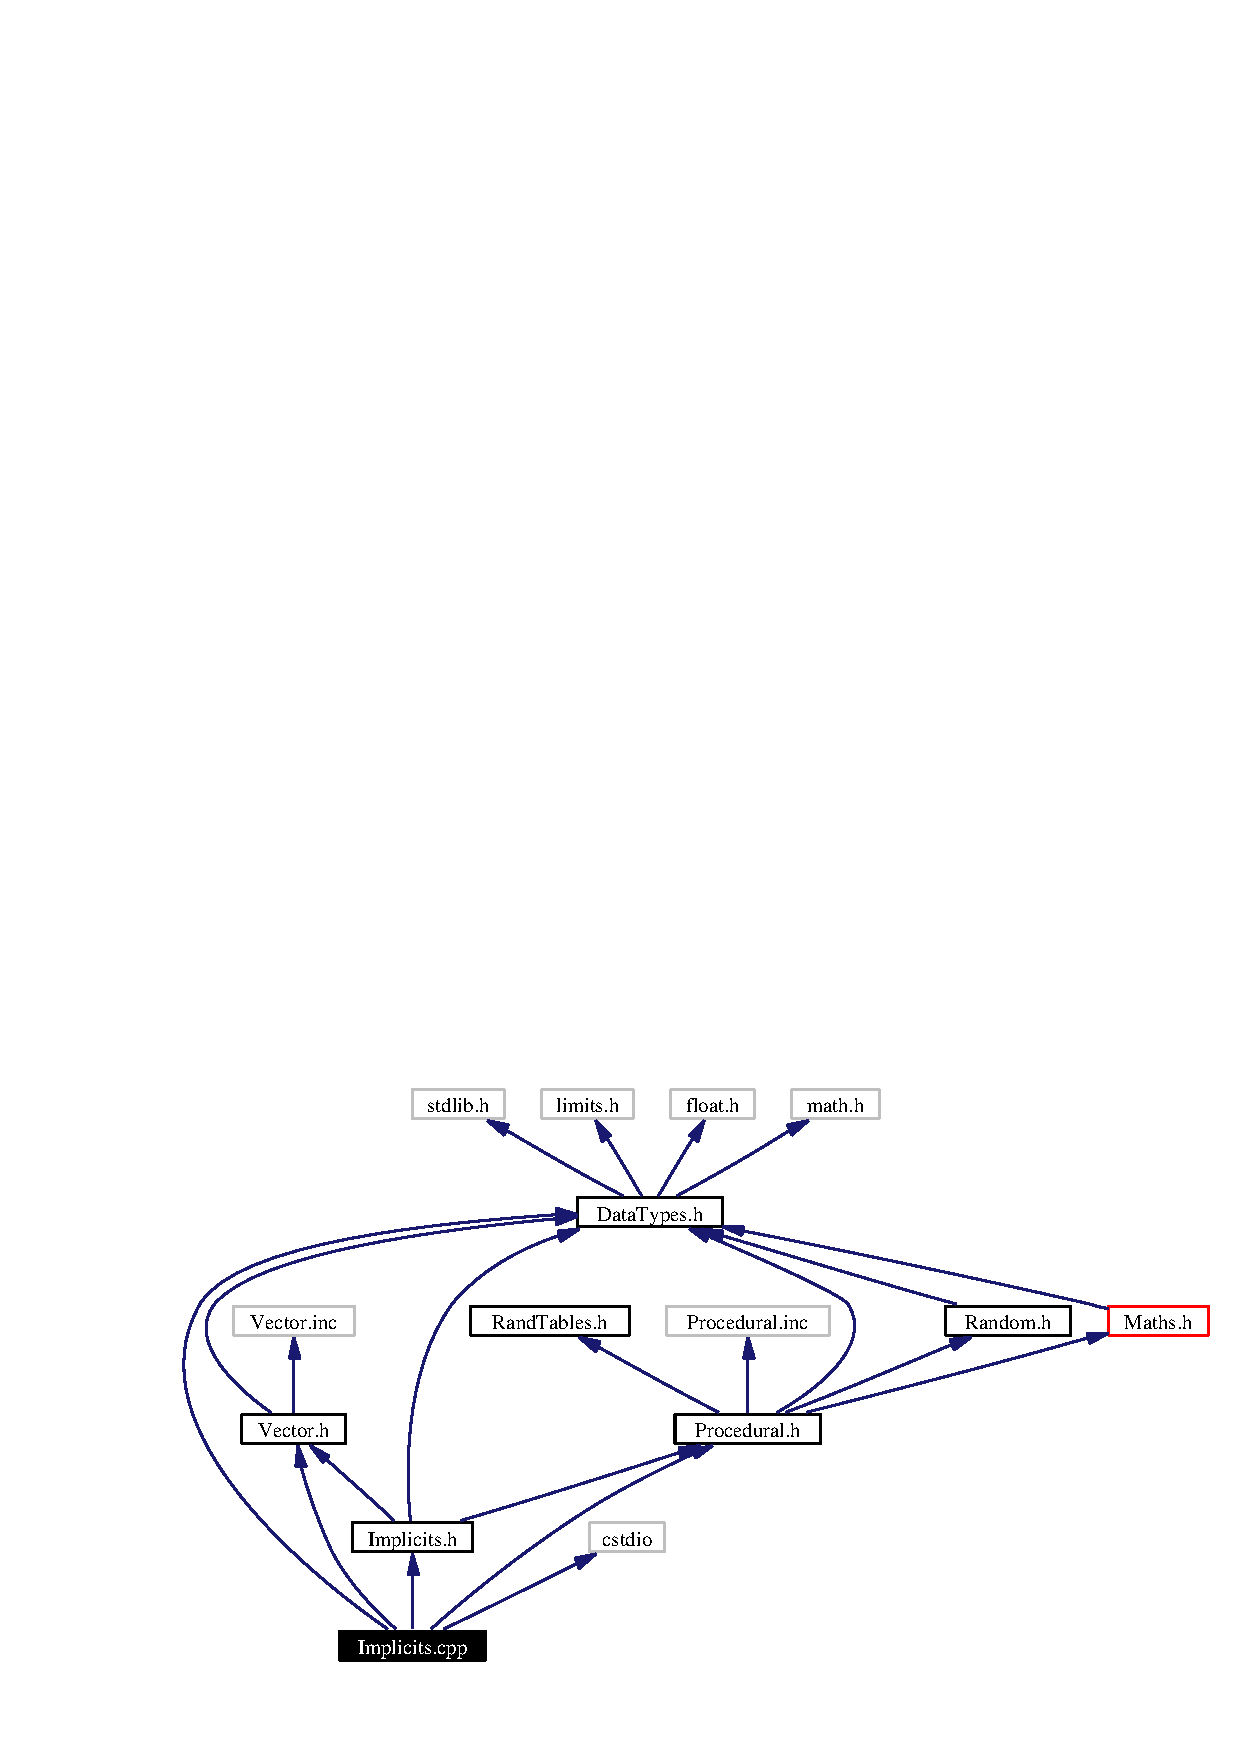
\includegraphics[width=290pt]{Implicits_8cpp__incl}
\end{center}
\end{figure}

\section{Implicits.h File Reference}
\label{Implicits_8h}\index{Implicits.h@{Implicits.h}}
{\tt \#include \char`\"{}Data\-Types.h\char`\"{}}\par
{\tt \#include \char`\"{}Procedural.h\char`\"{}}\par
{\tt \#include \char`\"{}Vector.h\char`\"{}}\par


Include dependency graph for Implicits.h:\begin{figure}[H]
\begin{center}
\leavevmode
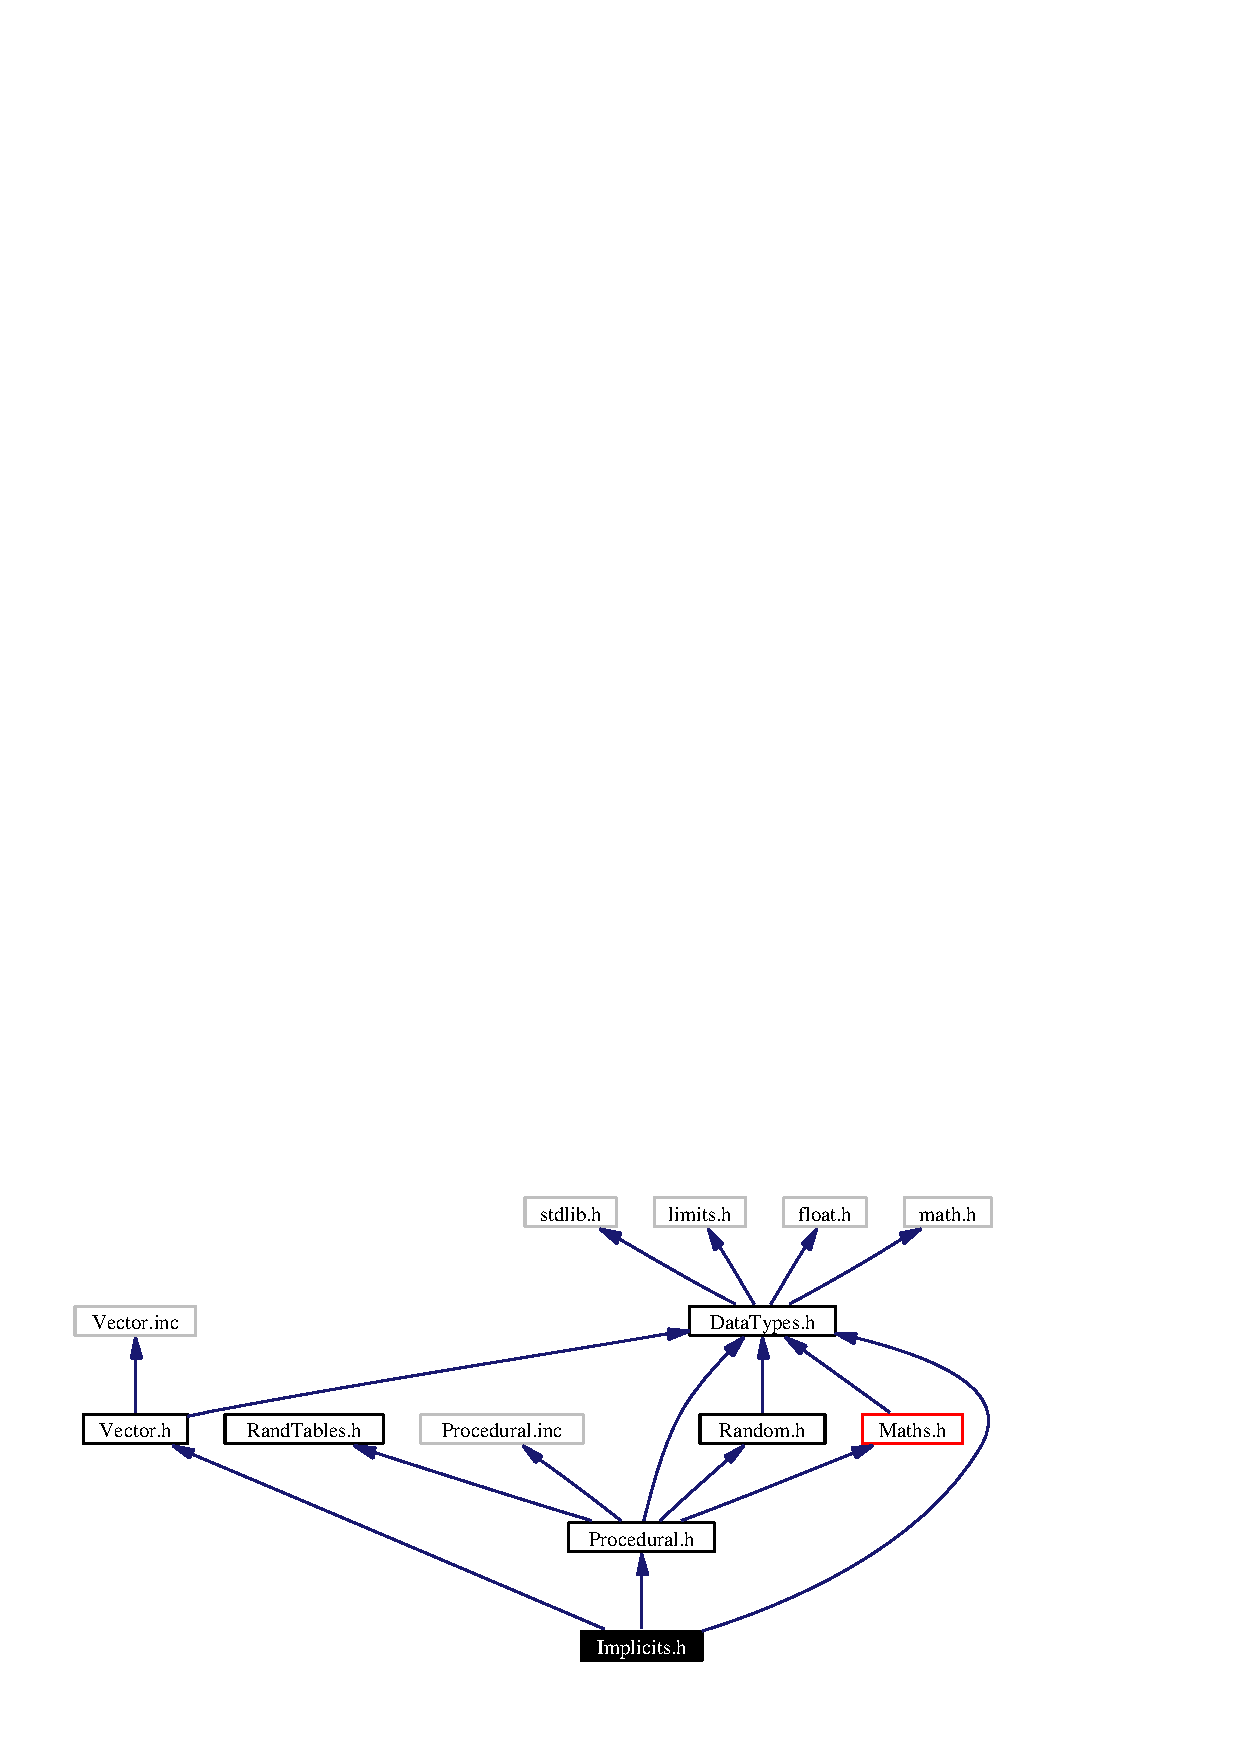
\includegraphics[width=250pt]{Implicits_8h__incl}
\end{center}
\end{figure}


This graph shows which files directly or indirectly include this file:\begin{figure}[H]
\begin{center}
\leavevmode
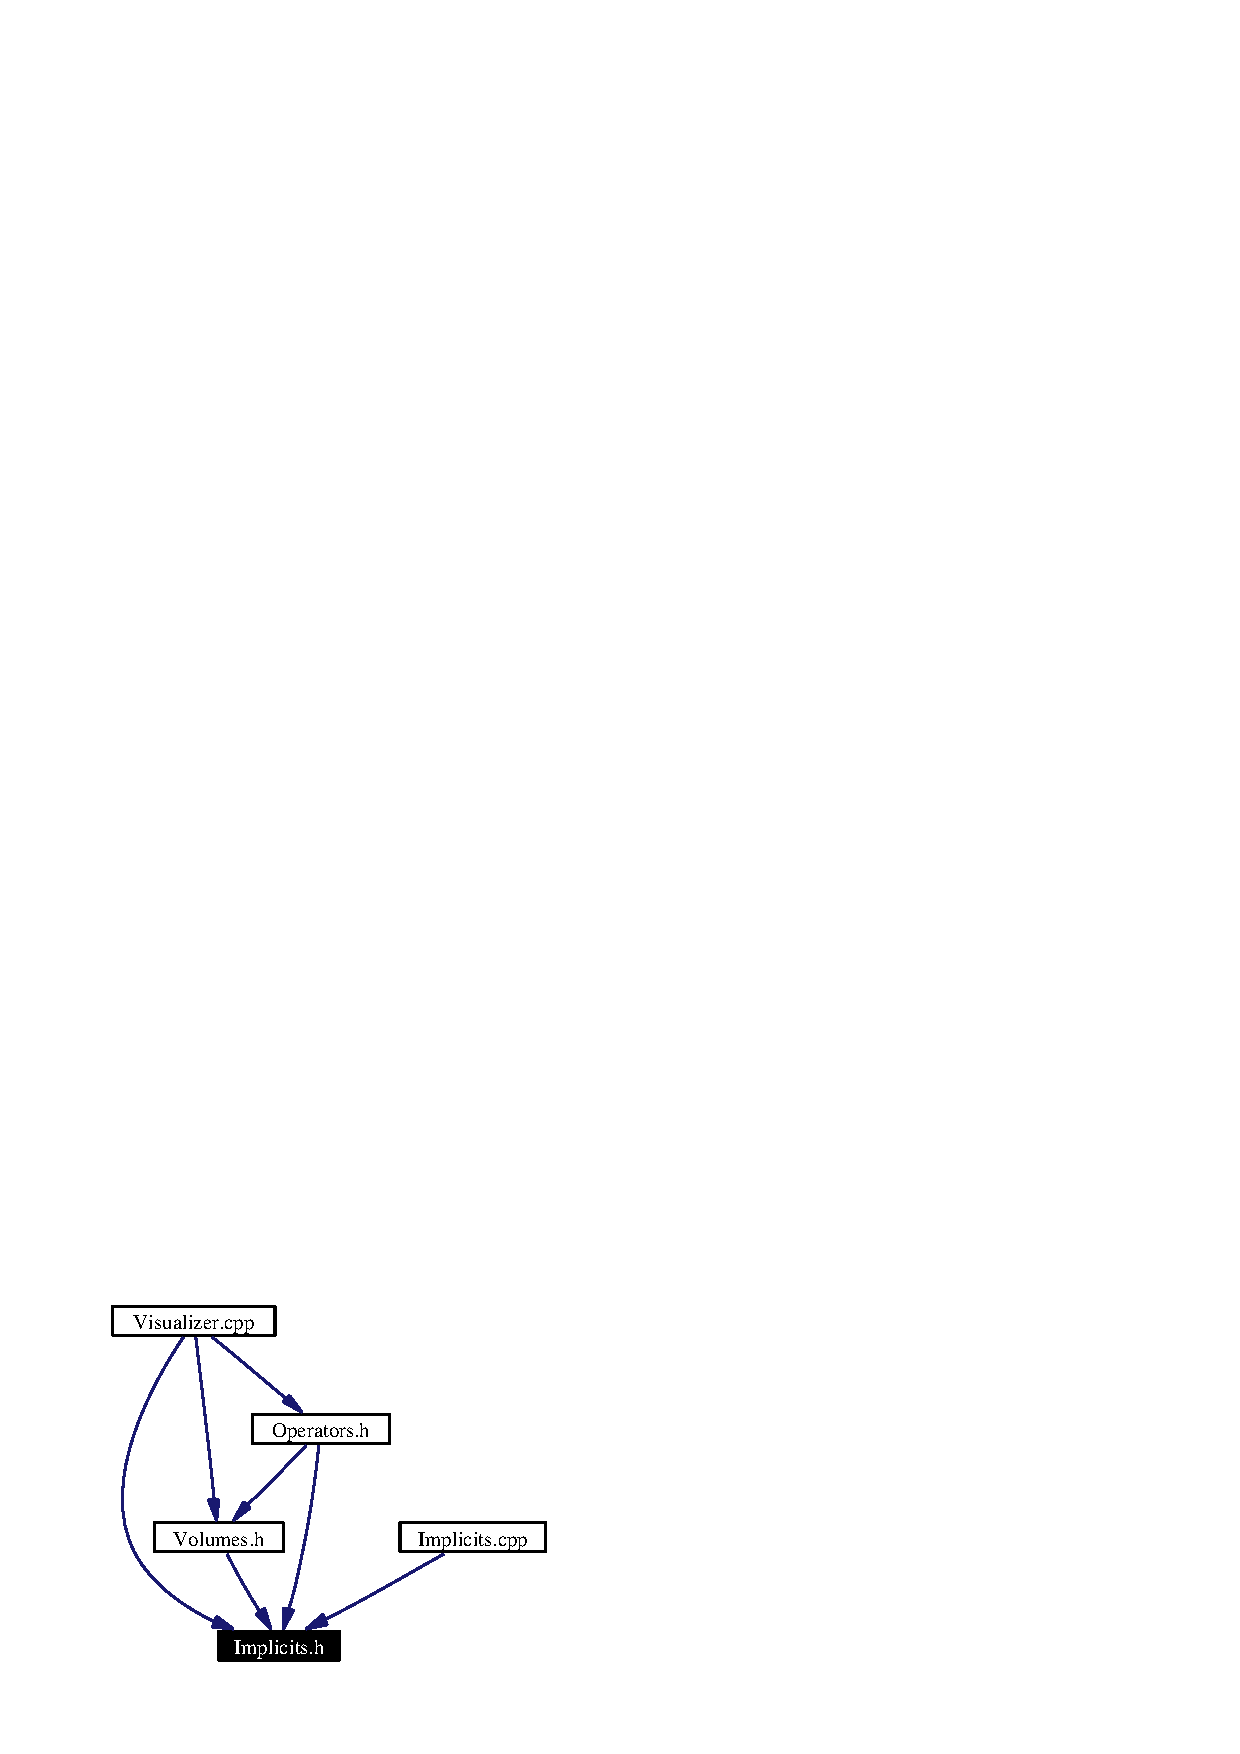
\includegraphics[width=131pt]{Implicits_8h__dep__incl}
\end{center}
\end{figure}
\subsection*{Namespaces}
\begin{CompactItemize}
\item 
namespace {\bf dg}
\end{CompactItemize}

\section{Key\-Bindings.h File Reference}
\label{KeyBindings_8h}\index{KeyBindings.h@{KeyBindings.h}}


This graph shows which files directly or indirectly include this file:\begin{figure}[H]
\begin{center}
\leavevmode
\includegraphics[width=171pt]{KeyBindings_8h__dep__incl}
\end{center}
\end{figure}

\section{Maths.cpp File Reference}
\label{Maths_8cpp}\index{Maths.cpp@{Maths.cpp}}
{\tt \#include \char`\"{}Data\-Types.h\char`\"{}}\par
{\tt \#include \char`\"{}Maths.h\char`\"{}}\par
{\tt \#include $<$cmath$>$}\par


Include dependency graph for Maths.cpp:\begin{figure}[H]
\begin{center}
\leavevmode
\includegraphics[width=130pt]{Maths_8cpp__incl}
\end{center}
\end{figure}

\section{Maths.h File Reference}
\label{Maths_8h}\index{Maths.h@{Maths.h}}
{\tt \#include \char`\"{}Data\-Types.h\char`\"{}}\par
{\tt \#include \char`\"{}Maths.inc\char`\"{}}\par


Include dependency graph for Maths.h:\begin{figure}[H]
\begin{center}
\leavevmode
\includegraphics[width=130pt]{Maths_8h__incl}
\end{center}
\end{figure}


This graph shows which files directly or indirectly include this file:\begin{figure}[H]
\begin{center}
\leavevmode
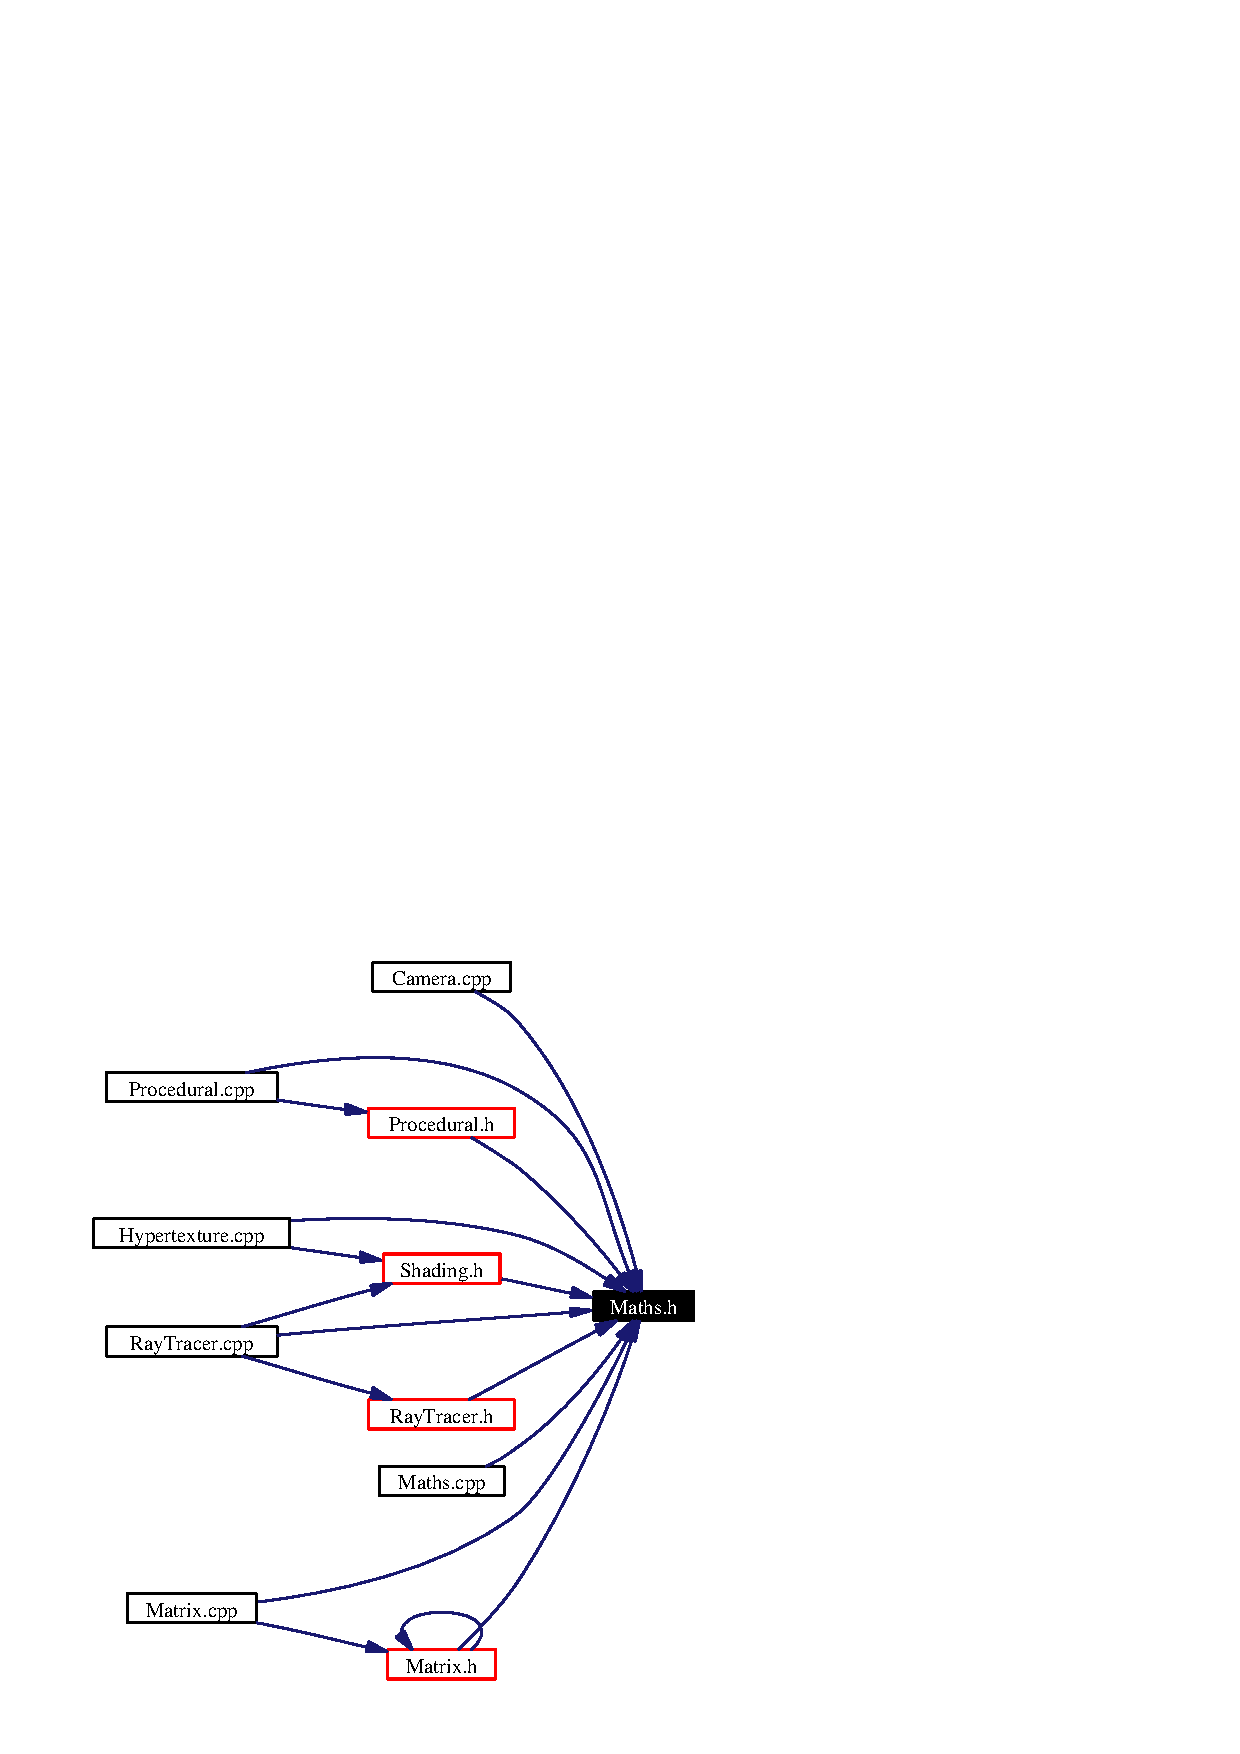
\includegraphics[width=171pt]{Maths_8h__dep__incl}
\end{center}
\end{figure}
\subsection*{Namespaces}
\begin{CompactItemize}
\item 
namespace {\bf dg}
\end{CompactItemize}

\section{Matrix.cpp File Reference}
\label{Matrix_8cpp}\index{Matrix.cpp@{Matrix.cpp}}
{\tt \#include \char`\"{}Matrix.h\char`\"{}}\par
{\tt \#include \char`\"{}Data\-Types.h\char`\"{}}\par
{\tt \#include \char`\"{}Maths.h\char`\"{}}\par
{\tt \#include \char`\"{}Vector.h\char`\"{}}\par
{\tt \#include $<$memory$>$}\par
{\tt \#include $<$algorithm$>$}\par


Include dependency graph for Matrix.cpp:\begin{figure}[H]
\begin{center}
\leavevmode
\includegraphics[width=190pt]{Matrix_8cpp__incl}
\end{center}
\end{figure}

\section{Matrix.h File Reference}
\label{Matrix_8h}\index{Matrix.h@{Matrix.h}}
{\tt \#include \char`\"{}Data\-Types.h\char`\"{}}\par
{\tt \#include \char`\"{}Maths.h\char`\"{}}\par
{\tt \#include \char`\"{}Vector.h\char`\"{}}\par
{\tt \#include \char`\"{}Matrix.h\char`\"{}}\par
{\tt \#include \char`\"{}Matrix.inc\char`\"{}}\par


Include dependency graph for Matrix.h:\begin{figure}[H]
\begin{center}
\leavevmode
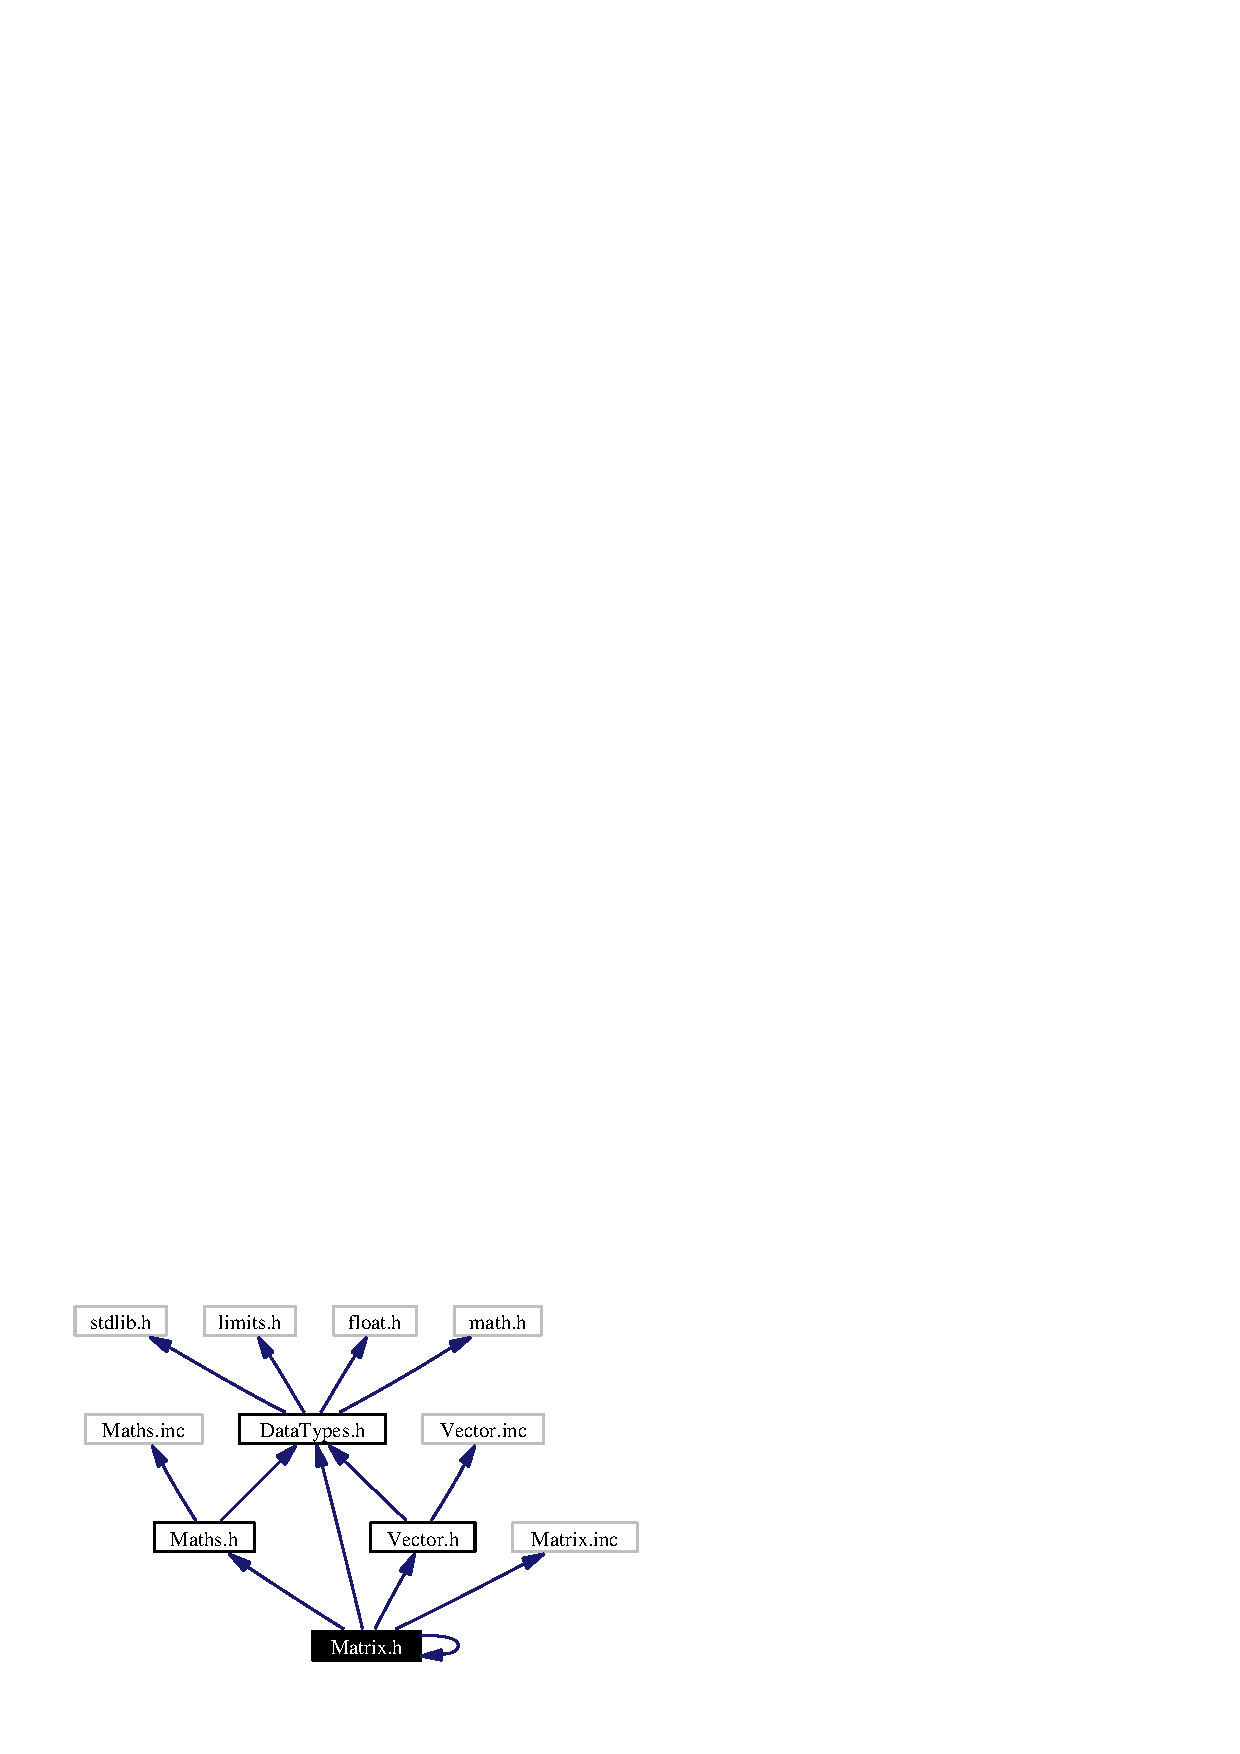
\includegraphics[width=153pt]{Matrix_8h__incl}
\end{center}
\end{figure}


This graph shows which files directly or indirectly include this file:\begin{figure}[H]
\begin{center}
\leavevmode
\includegraphics[width=97pt]{Matrix_8h__dep__incl}
\end{center}
\end{figure}
\subsection*{Namespaces}
\begin{CompactItemize}
\item 
namespace {\bf dg}
\end{CompactItemize}

\section{Messages.cpp File Reference}
\label{Messages_8cpp}\index{Messages.cpp@{Messages.cpp}}
{\tt \#include \char`\"{}Messages.h\char`\"{}}\par
{\tt \#include $<$cstdio$>$}\par
{\tt \#include $<$cstdlib$>$}\par


Include dependency graph for Messages.cpp:\begin{figure}[H]
\begin{center}
\leavevmode
\includegraphics[width=101pt]{Messages_8cpp__incl}
\end{center}
\end{figure}

\section{Messages.h File Reference}
\label{Messages_8h}\index{Messages.h@{Messages.h}}
{\tt \#include $<$cstdio$>$}\par
{\tt \#include $<$cstdarg$>$}\par


Include dependency graph for Messages.h:\begin{figure}[H]
\begin{center}
\leavevmode
\includegraphics[width=67pt]{Messages_8h__incl}
\end{center}
\end{figure}


This graph shows which files directly or indirectly include this file:\begin{figure}[H]
\begin{center}
\leavevmode
\includegraphics[width=105pt]{Messages_8h__dep__incl}
\end{center}
\end{figure}
\subsection*{Namespaces}
\begin{CompactItemize}
\item 
namespace {\bf dg}
\end{CompactItemize}
\subsection*{Defines}
\begin{CompactItemize}
\item 
\#define {\bf PRINT\_\-FUNC}
\end{CompactItemize}


\subsection{Define Documentation}
\index{Messages.h@{Messages.h}!PRINT_FUNC@{PRINT\_\-FUNC}}
\index{PRINT_FUNC@{PRINT\_\-FUNC}!Messages.h@{Messages.h}}
\subsubsection{\setlength{\rightskip}{0pt plus 5cm}\#define PRINT\_\-FUNC}\label{Messages_8h_a0}




Definition at line 30 of file Messages.h.
\section{Open\-GLHeaders.h File Reference}
\label{OpenGLHeaders_8h}\index{OpenGLHeaders.h@{OpenGLHeaders.h}}
{\tt \#include $<$GL/gl.h$>$}\par
{\tt \#include $<$GL/glu.h$>$}\par


Include dependency graph for Open\-GLHeaders.h:\begin{figure}[H]
\begin{center}
\leavevmode
\includegraphics[width=77pt]{OpenGLHeaders_8h__incl}
\end{center}
\end{figure}


This graph shows which files directly or indirectly include this file:\begin{figure}[H]
\begin{center}
\leavevmode
\includegraphics[width=137pt]{OpenGLHeaders_8h__dep__incl}
\end{center}
\end{figure}

\section{Operators.h File Reference}
\label{Operators_8h}\index{Operators.h@{Operators.h}}
{\tt \#include \char`\"{}Data\-Types.h\char`\"{}}\par
{\tt \#include \char`\"{}Volumes.h\char`\"{}}\par
{\tt \#include \char`\"{}Implicits.h\char`\"{}}\par
{\tt \#include \char`\"{}Procedural.h\char`\"{}}\par


Include dependency graph for Operators.h:\begin{figure}[H]
\begin{center}
\leavevmode
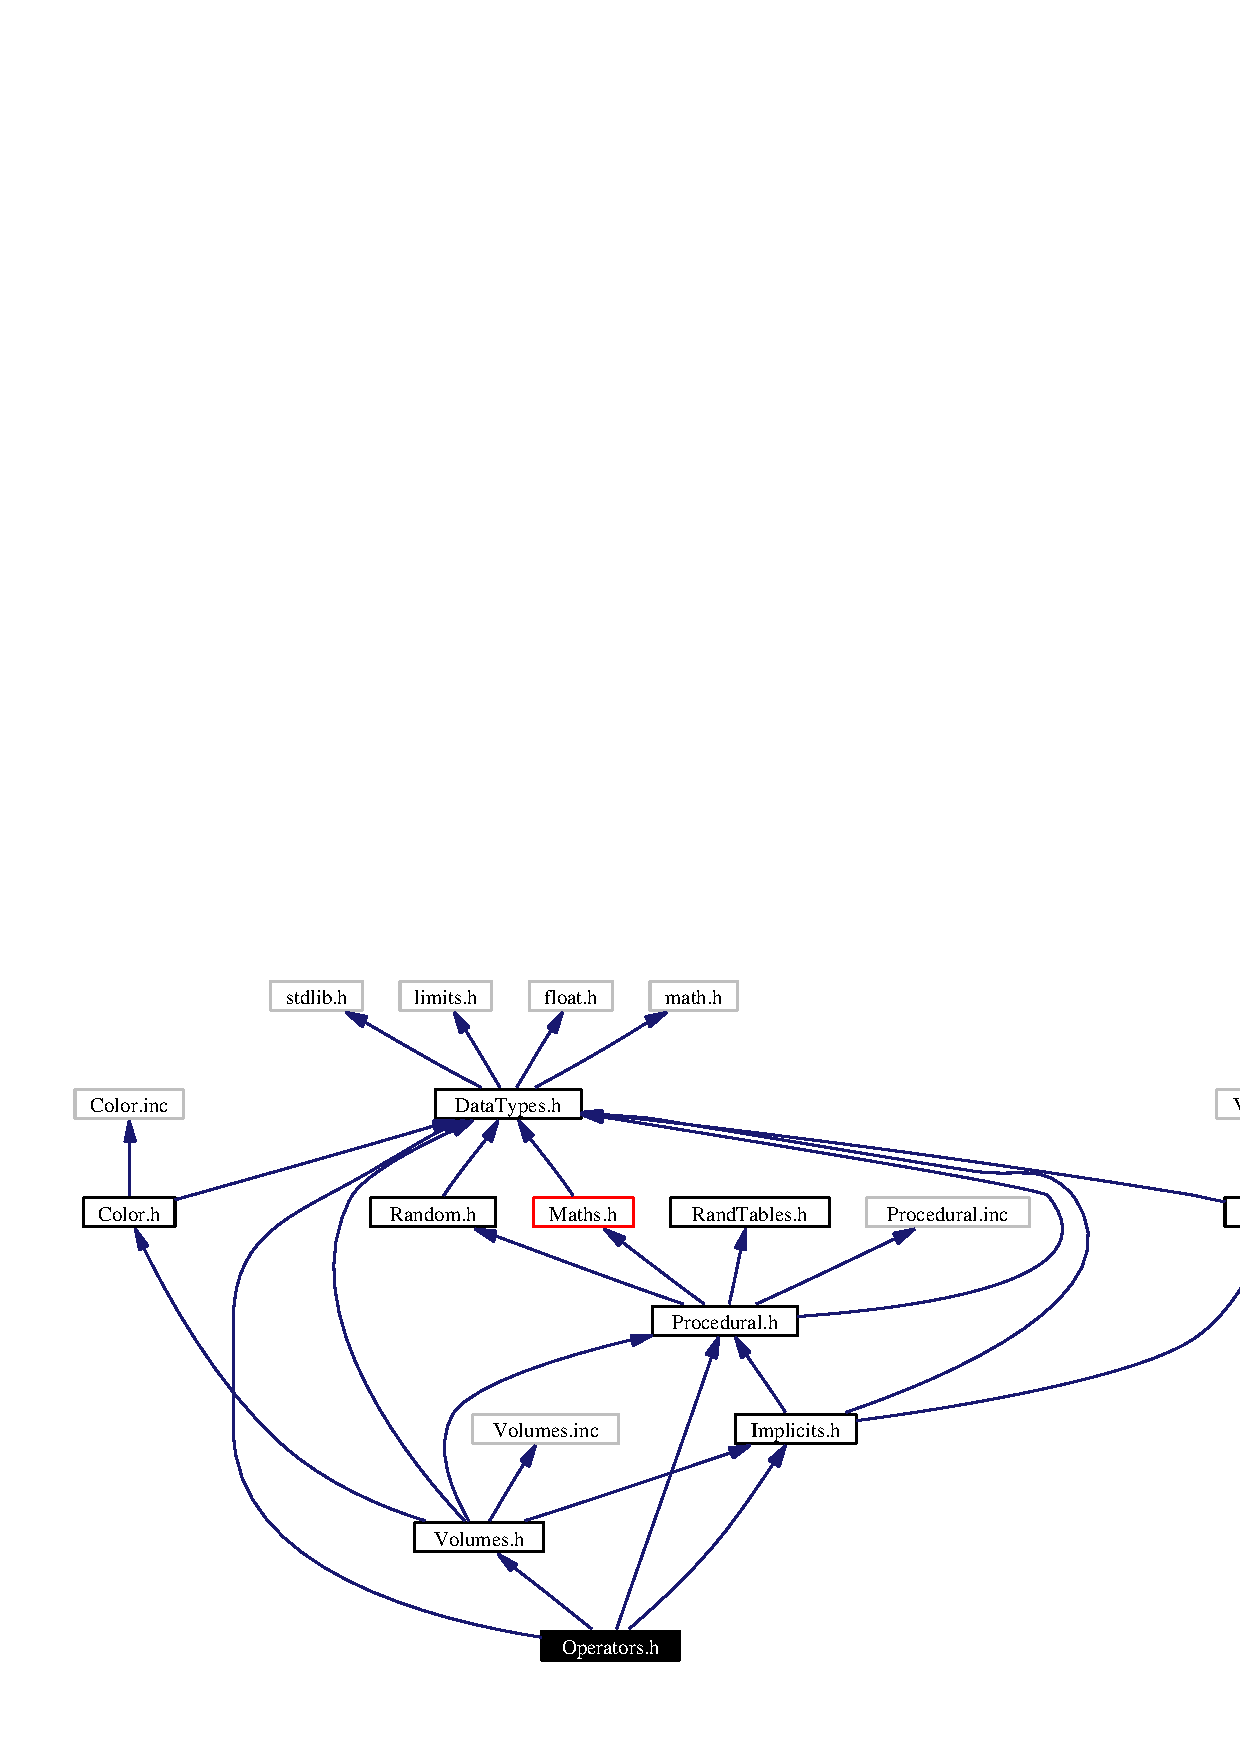
\includegraphics[width=321pt]{Operators_8h__incl}
\end{center}
\end{figure}


This graph shows which files directly or indirectly include this file:\begin{figure}[H]
\begin{center}
\leavevmode
\includegraphics[width=113pt]{Operators_8h__dep__incl}
\end{center}
\end{figure}
\subsection*{Namespaces}
\begin{CompactItemize}
\item 
namespace {\bf dg}
\end{CompactItemize}

\section{Polygonizer.cpp File Reference}
\label{Polygonizer_8cpp}\index{Polygonizer.cpp@{Polygonizer.cpp}}
{\tt \#include \char`\"{}Data\-Types.h\char`\"{}}\par
{\tt \#include \char`\"{}Polygonizer.h\char`\"{}}\par
{\tt \#include \char`\"{}Shading.h\char`\"{}}\par


Include dependency graph for Polygonizer.cpp:\begin{figure}[H]
\begin{center}
\leavevmode
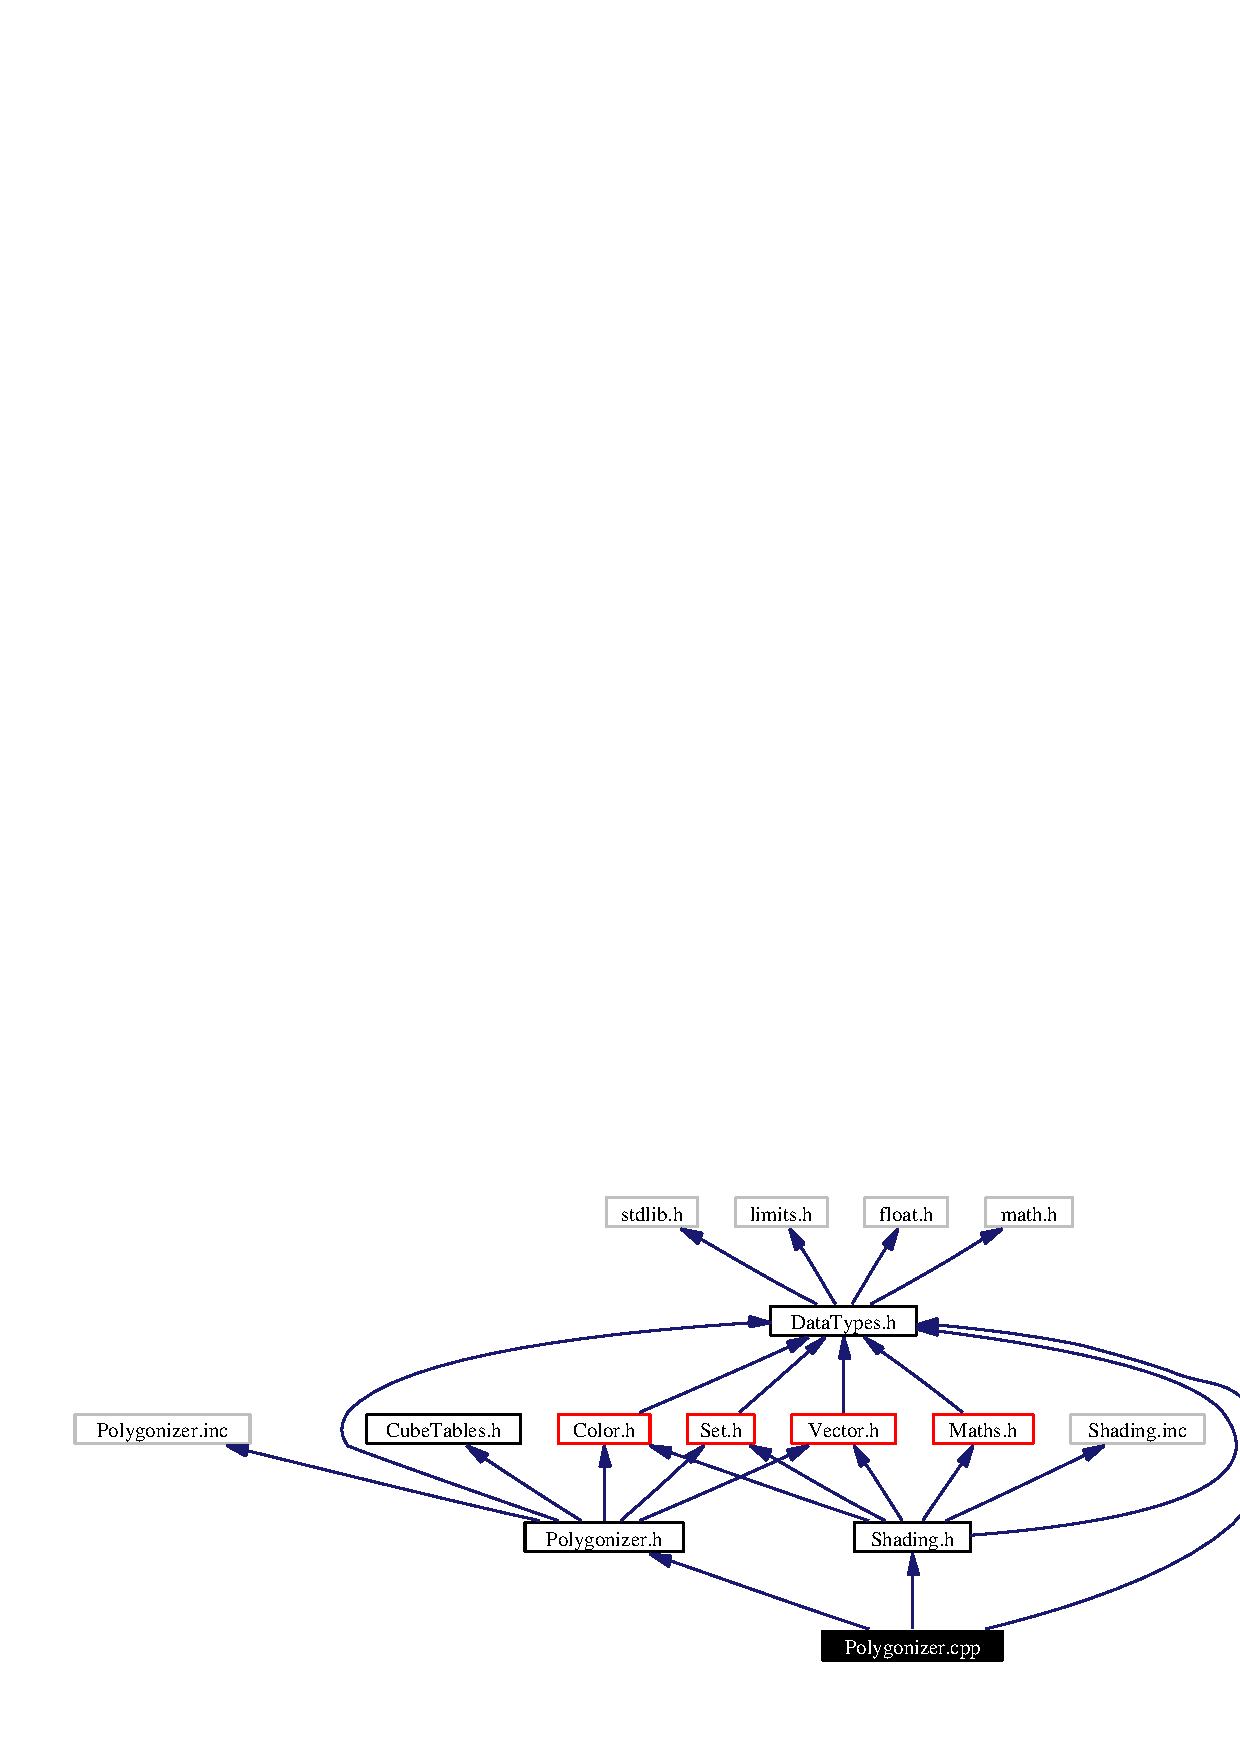
\includegraphics[width=327pt]{Polygonizer_8cpp__incl}
\end{center}
\end{figure}

\section{Polygonizer.h File Reference}
\label{Polygonizer_8h}\index{Polygonizer.h@{Polygonizer.h}}
{\tt \#include \char`\"{}Data\-Types.h\char`\"{}}\par
{\tt \#include \char`\"{}Cube\-Tables.h\char`\"{}}\par
{\tt \#include \char`\"{}Vector.h\char`\"{}}\par
{\tt \#include \char`\"{}Color.h\char`\"{}}\par
{\tt \#include \char`\"{}Set.h\char`\"{}}\par
{\tt \#include \char`\"{}Polygonizer.inc\char`\"{}}\par


Include dependency graph for Polygonizer.h:\begin{figure}[H]
\begin{center}
\leavevmode
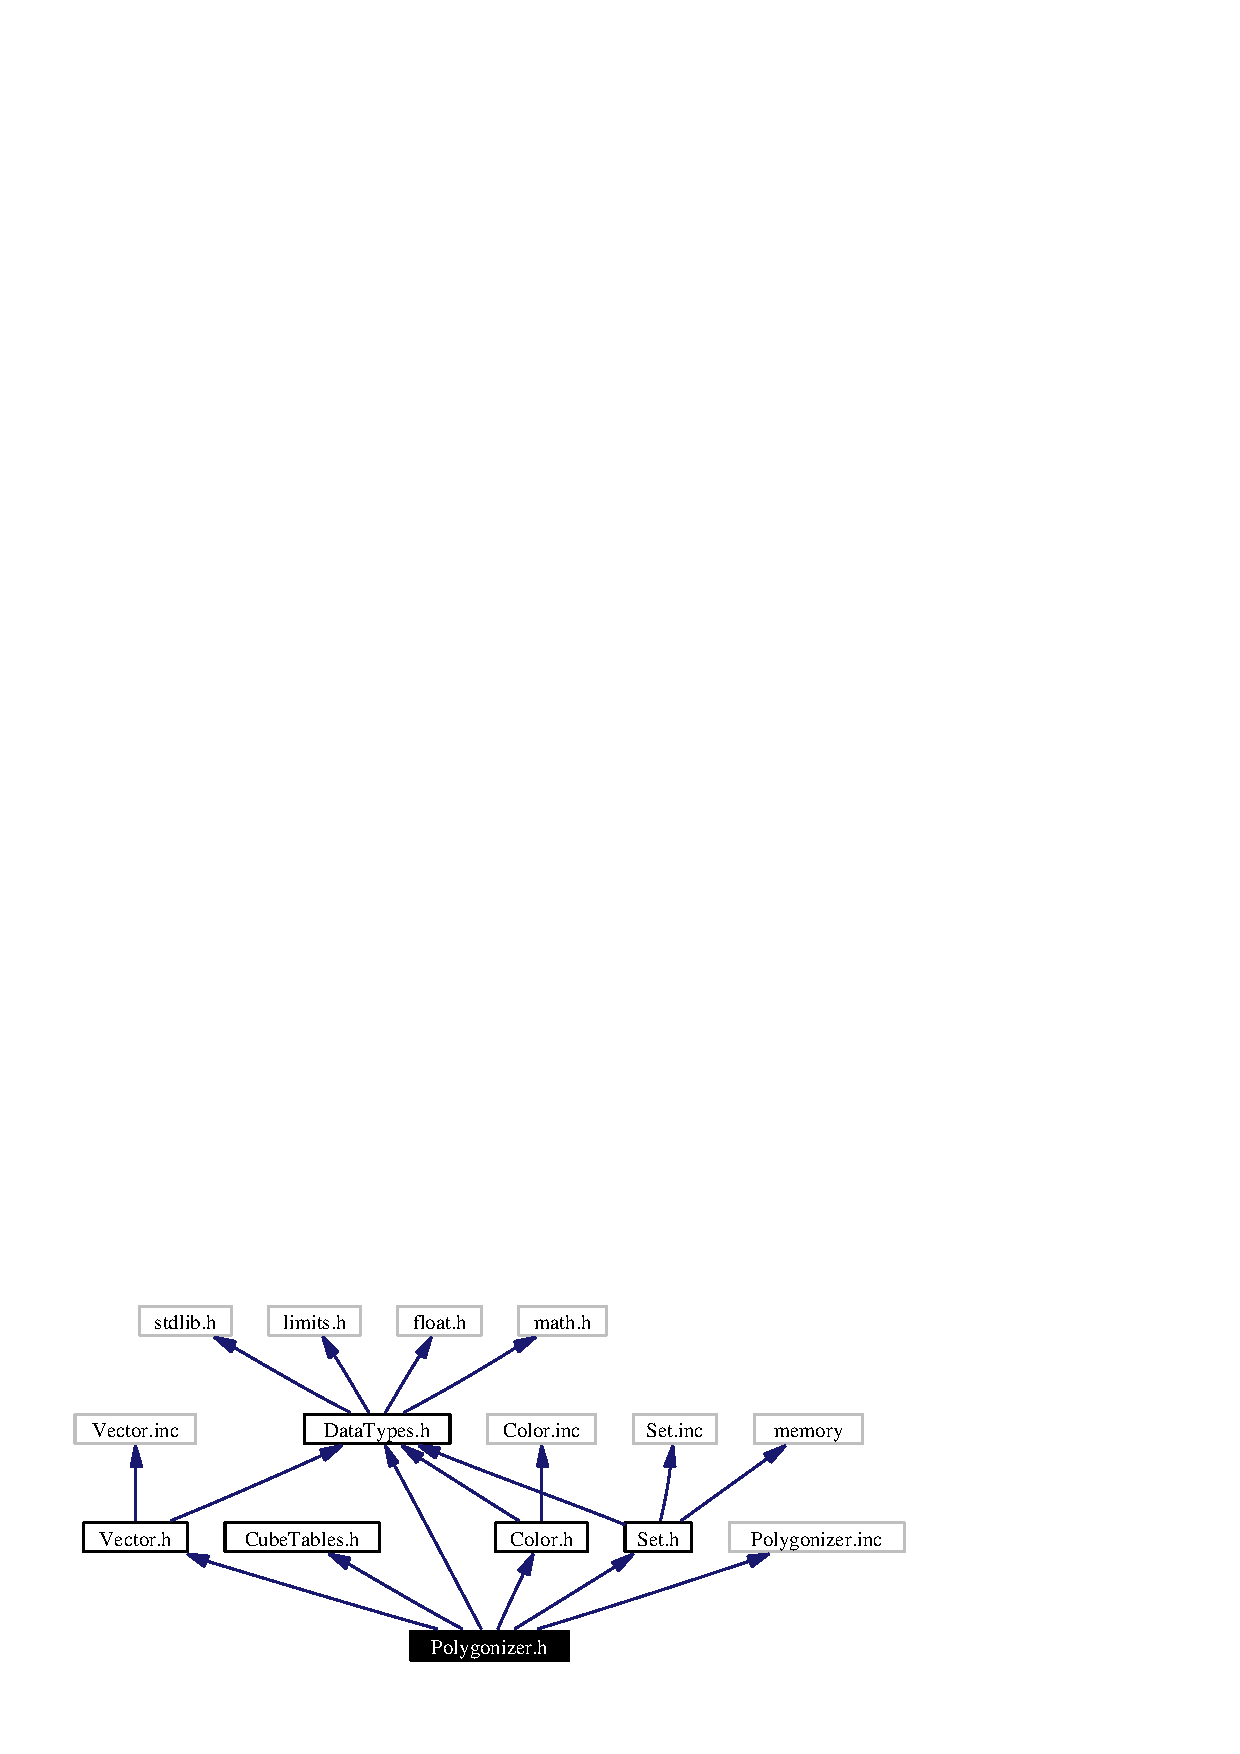
\includegraphics[width=217pt]{Polygonizer_8h__incl}
\end{center}
\end{figure}


This graph shows which files directly or indirectly include this file:\begin{figure}[H]
\begin{center}
\leavevmode
\includegraphics[width=106pt]{Polygonizer_8h__dep__incl}
\end{center}
\end{figure}
\subsection*{Namespaces}
\begin{CompactItemize}
\item 
namespace {\bf dg}
\end{CompactItemize}

\section{Procedural.cpp File Reference}
\label{Procedural_8cpp}\index{Procedural.cpp@{Procedural.cpp}}
{\tt \#include \char`\"{}Procedural.h\char`\"{}}\par
{\tt \#include \char`\"{}Data\-Types.h\char`\"{}}\par
{\tt \#include \char`\"{}Rand\-Tables.h\char`\"{}}\par
{\tt \#include \char`\"{}Messages.h\char`\"{}}\par
{\tt \#include \char`\"{}Maths.h\char`\"{}}\par


Include dependency graph for Procedural.cpp:\begin{figure}[H]
\begin{center}
\leavevmode
\includegraphics[width=277pt]{Procedural_8cpp__incl}
\end{center}
\end{figure}

\section{Procedural.h File Reference}
\label{Procedural_8h}\index{Procedural.h@{Procedural.h}}
{\tt \#include \char`\"{}Data\-Types.h\char`\"{}}\par
{\tt \#include \char`\"{}Rand\-Tables.h\char`\"{}}\par
{\tt \#include \char`\"{}Random.h\char`\"{}}\par
{\tt \#include \char`\"{}Maths.h\char`\"{}}\par
{\tt \#include \char`\"{}Procedural.inc\char`\"{}}\par


Include dependency graph for Procedural.h:\begin{figure}[H]
\begin{center}
\leavevmode
\includegraphics[width=207pt]{Procedural_8h__incl}
\end{center}
\end{figure}


This graph shows which files directly or indirectly include this file:\begin{figure}[H]
\begin{center}
\leavevmode
\includegraphics[width=202pt]{Procedural_8h__dep__incl}
\end{center}
\end{figure}
\subsection*{Namespaces}
\begin{CompactItemize}
\item 
namespace {\bf dg}
\end{CompactItemize}

\section{Random.cpp File Reference}
\label{Random_8cpp}\index{Random.cpp@{Random.cpp}}
{\tt \#include \char`\"{}Random.h\char`\"{}}\par


Include dependency graph for Random.cpp:\begin{figure}[H]
\begin{center}
\leavevmode
\includegraphics[width=54pt]{Random_8cpp__incl}
\end{center}
\end{figure}
\subsection*{Defines}
\begin{CompactItemize}
\item 
\#define {\bf N}\ 624
\item 
\#define {\bf M}\ 397
\item 
\#define {\bf MATRIX\_\-A}\ 0x9908b0df\-UL
\item 
\#define {\bf UPPER\_\-MASK}\ 0x80000000UL
\item 
\#define {\bf LOWER\_\-MASK}\ 0x7fffffff\-UL
\end{CompactItemize}


\subsection{Define Documentation}
\index{Random.cpp@{Random.cpp}!LOWER_MASK@{LOWER\_\-MASK}}
\index{LOWER_MASK@{LOWER\_\-MASK}!Random.cpp@{Random.cpp}}
\subsubsection{\setlength{\rightskip}{0pt plus 5cm}\#define LOWER\_\-MASK\ 0x7fffffff\-UL}\label{Random_8cpp_a4}




Definition at line 41 of file Random.cpp.

Referenced by dg::Random\-Int().\index{Random.cpp@{Random.cpp}!M@{M}}
\index{M@{M}!Random.cpp@{Random.cpp}}
\subsubsection{\setlength{\rightskip}{0pt plus 5cm}\#define M\ 397}\label{Random_8cpp_a1}




Definition at line 38 of file Random.cpp.

Referenced by dg::Random\-Int().\index{Random.cpp@{Random.cpp}!MATRIX_A@{MATRIX\_\-A}}
\index{MATRIX_A@{MATRIX\_\-A}!Random.cpp@{Random.cpp}}
\subsubsection{\setlength{\rightskip}{0pt plus 5cm}\#define MATRIX\_\-A\ 0x9908b0df\-UL}\label{Random_8cpp_a2}




Definition at line 39 of file Random.cpp.

Referenced by dg::Random\-Int().\index{Random.cpp@{Random.cpp}!N@{N}}
\index{N@{N}!Random.cpp@{Random.cpp}}
\subsubsection{\setlength{\rightskip}{0pt plus 5cm}\#define N\ 624}\label{Random_8cpp_a0}




Definition at line 37 of file Random.cpp.

Referenced by dg::Random\-Int(), and dg::Seed\-Random().\index{Random.cpp@{Random.cpp}!UPPER_MASK@{UPPER\_\-MASK}}
\index{UPPER_MASK@{UPPER\_\-MASK}!Random.cpp@{Random.cpp}}
\subsubsection{\setlength{\rightskip}{0pt plus 5cm}\#define UPPER\_\-MASK\ 0x80000000UL}\label{Random_8cpp_a3}




Definition at line 40 of file Random.cpp.

Referenced by dg::Random\-Int().
\section{Random.h File Reference}
\label{Random_8h}\index{Random.h@{Random.h}}
{\tt \#include \char`\"{}Data\-Types.h\char`\"{}}\par


Include dependency graph for Random.h:\begin{figure}[H]
\begin{center}
\leavevmode
\includegraphics[width=130pt]{Random_8h__incl}
\end{center}
\end{figure}


This graph shows which files directly or indirectly include this file:\begin{figure}[H]
\begin{center}
\leavevmode
\includegraphics[width=242pt]{Random_8h__dep__incl}
\end{center}
\end{figure}
\subsection*{Namespaces}
\begin{CompactItemize}
\item 
namespace {\bf dg}
\end{CompactItemize}

\section{Rand\-Tables.h File Reference}
\label{RandTables_8h}\index{RandTables.h@{RandTables.h}}


This graph shows which files directly or indirectly include this file:\begin{figure}[H]
\begin{center}
\leavevmode
\includegraphics[width=170pt]{RandTables_8h__dep__incl}
\end{center}
\end{figure}
\subsection*{Namespaces}
\begin{CompactItemize}
\item 
namespace {\bf dg}
\end{CompactItemize}

\section{Ray\-Tracer.cpp File Reference}
\label{RayTracer_8cpp}\index{RayTracer.cpp@{RayTracer.cpp}}
{\tt \#include \char`\"{}Ray\-Tracer.h\char`\"{}}\par
{\tt \#include \char`\"{}Maths.h\char`\"{}}\par
{\tt \#include \char`\"{}Shading.h\char`\"{}}\par
{\tt \#include $<$memory$>$}\par


Include dependency graph for Ray\-Tracer.cpp:\begin{figure}[H]
\begin{center}
\leavevmode
\includegraphics[width=363pt]{RayTracer_8cpp__incl}
\end{center}
\end{figure}

\section{Ray\-Tracer.h File Reference}
\label{RayTracer_8h}\index{RayTracer.h@{RayTracer.h}}
{\tt \#include \char`\"{}Data\-Types.h\char`\"{}}\par
{\tt \#include \char`\"{}Camera.h\char`\"{}}\par
{\tt \#include \char`\"{}Vector.h\char`\"{}}\par
{\tt \#include \char`\"{}Color.h\char`\"{}}\par
{\tt \#include \char`\"{}Maths.h\char`\"{}}\par
{\tt \#include \char`\"{}Ray\-Tracer.inc\char`\"{}}\par


Include dependency graph for Ray\-Tracer.h:\begin{figure}[H]
\begin{center}
\leavevmode
\includegraphics[width=260pt]{RayTracer_8h__incl}
\end{center}
\end{figure}


This graph shows which files directly or indirectly include this file:\begin{figure}[H]
\begin{center}
\leavevmode
\includegraphics[width=104pt]{RayTracer_8h__dep__incl}
\end{center}
\end{figure}
\subsection*{Namespaces}
\begin{CompactItemize}
\item 
namespace {\bf dg}
\end{CompactItemize}

\section{Set.cpp File Reference}
\label{Set_8cpp}\index{Set.cpp@{Set.cpp}}
{\tt \#include \char`\"{}Set.h\char`\"{}}\par


Include dependency graph for Set.cpp:\begin{figure}[H]
\begin{center}
\leavevmode
\includegraphics[width=117pt]{Set_8cpp__incl}
\end{center}
\end{figure}

\section{Set.h File Reference}
\label{Set_8h}\index{Set.h@{Set.h}}
{\tt \#include \char`\"{}Data\-Types.h\char`\"{}}\par
{\tt \#include $<$memory$>$}\par
{\tt \#include \char`\"{}Set.inc\char`\"{}}\par


Include dependency graph for Set.h:\begin{figure}[H]
\begin{center}
\leavevmode
\includegraphics[width=157pt]{Set_8h__incl}
\end{center}
\end{figure}


This graph shows which files directly or indirectly include this file:\begin{figure}[H]
\begin{center}
\leavevmode
\includegraphics[width=271pt]{Set_8h__dep__incl}
\end{center}
\end{figure}
\subsection*{Namespaces}
\begin{CompactItemize}
\item 
namespace {\bf dg}
\end{CompactItemize}

\section{Shading.cpp File Reference}
\label{Shading_8cpp}\index{Shading.cpp@{Shading.cpp}}
{\tt \#include \char`\"{}Shading.h\char`\"{}}\par


Include dependency graph for Shading.cpp:\begin{figure}[H]
\begin{center}
\leavevmode
\includegraphics[width=192pt]{Shading_8cpp__incl}
\end{center}
\end{figure}

\section{Shading.h File Reference}
\label{Shading_8h}\index{Shading.h@{Shading.h}}
{\tt \#include \char`\"{}Data\-Types.h\char`\"{}}\par
{\tt \#include \char`\"{}Vector.h\char`\"{}}\par
{\tt \#include \char`\"{}Color.h\char`\"{}}\par
{\tt \#include \char`\"{}Maths.h\char`\"{}}\par
{\tt \#include \char`\"{}Set.h\char`\"{}}\par
{\tt \#include \char`\"{}Shading.inc\char`\"{}}\par


Include dependency graph for Shading.h:\begin{figure}[H]
\begin{center}
\leavevmode
\includegraphics[width=227pt]{Shading_8h__incl}
\end{center}
\end{figure}


This graph shows which files directly or indirectly include this file:\begin{figure}[H]
\begin{center}
\leavevmode
\includegraphics[width=258pt]{Shading_8h__dep__incl}
\end{center}
\end{figure}
\subsection*{Namespaces}
\begin{CompactItemize}
\item 
namespace {\bf dg}
\end{CompactItemize}

\section{Timer.cpp File Reference}
\label{Timer_8cpp}\index{Timer.cpp@{Timer.cpp}}
{\tt \#include \char`\"{}Timer.h\char`\"{}}\par
{\tt \#include $<$sys/time.h$>$}\par


Include dependency graph for Timer.cpp:\begin{figure}[H]
\begin{center}
\leavevmode
\includegraphics[width=125pt]{Timer_8cpp__incl}
\end{center}
\end{figure}

\section{Timer.h File Reference}
\label{Timer_8h}\index{Timer.h@{Timer.h}}
{\tt \#include \char`\"{}Data\-Types.h\char`\"{}}\par
{\tt \#include $<$memory$>$}\par
{\tt \#include \char`\"{}Timer.inc\char`\"{}}\par


Include dependency graph for Timer.h:\begin{figure}[H]
\begin{center}
\leavevmode
\includegraphics[width=165pt]{Timer_8h__incl}
\end{center}
\end{figure}


This graph shows which files directly or indirectly include this file:\begin{figure}[H]
\begin{center}
\leavevmode
\includegraphics[width=171pt]{Timer_8h__dep__incl}
\end{center}
\end{figure}
\subsection*{Namespaces}
\begin{CompactItemize}
\item 
namespace {\bf dg}
\end{CompactItemize}

\section{Vector.cpp File Reference}
\label{Vector_8cpp}\index{Vector.cpp@{Vector.cpp}}
{\tt \#include \char`\"{}Vector.h\char`\"{}}\par
{\tt \#include \char`\"{}Data\-Types.h\char`\"{}}\par


Include dependency graph for Vector.cpp:\begin{figure}[H]
\begin{center}
\leavevmode
\includegraphics[width=91pt]{Vector_8cpp__incl}
\end{center}
\end{figure}

\section{Vector.h File Reference}
\label{Vector_8h}\index{Vector.h@{Vector.h}}
{\tt \#include \char`\"{}Data\-Types.h\char`\"{}}\par
{\tt \#include \char`\"{}Vector.inc\char`\"{}}\par


Include dependency graph for Vector.h:\begin{figure}[H]
\begin{center}
\leavevmode
\includegraphics[width=131pt]{Vector_8h__incl}
\end{center}
\end{figure}


This graph shows which files directly or indirectly include this file:\begin{figure}[H]
\begin{center}
\leavevmode
\includegraphics[width=168pt]{Vector_8h__dep__incl}
\end{center}
\end{figure}
\subsection*{Namespaces}
\begin{CompactItemize}
\item 
namespace {\bf dg}
\end{CompactItemize}

\section{Visualizer.cpp File Reference}
\label{Visualizer_8cpp}\index{Visualizer.cpp@{Visualizer.cpp}}
{\tt \#include \char`\"{}Window.h\char`\"{}}\par
{\tt \#include \char`\"{}Implicits.h\char`\"{}}\par
{\tt \#include \char`\"{}Operators.h\char`\"{}}\par
{\tt \#include \char`\"{}Shading.h\char`\"{}}\par
{\tt \#include \char`\"{}Volumes.h\char`\"{}}\par
{\tt \#include \char`\"{}Visualizer.h\char`\"{}}\par
{\tt \#include \char`\"{}Glut\-Headers.h\char`\"{}}\par
{\tt \#include \char`\"{}Random.h\char`\"{}}\par
{\tt \#include \char`\"{}Matrix.h\char`\"{}}\par


Include dependency graph for Visualizer.cpp:\begin{figure}[H]
\begin{center}
\leavevmode
\includegraphics[width=220pt]{Visualizer_8cpp__incl}
\end{center}
\end{figure}
\subsection*{Variables}
\begin{CompactItemize}
\item 
Visualizer {\bf sk\-App}
\end{CompactItemize}


\subsection{Variable Documentation}
\index{Visualizer.cpp@{Visualizer.cpp}!skApp@{skApp}}
\index{skApp@{skApp}!Visualizer.cpp@{Visualizer.cpp}}
\subsubsection{\setlength{\rightskip}{0pt plus 5cm}Visualizer sk\-App}\label{Visualizer_8cpp_a0}




Definition at line 13 of file Visualizer.cpp.
\section{Visualizer.h File Reference}
\label{Visualizer_8h}\index{Visualizer.h@{Visualizer.h}}
{\tt \#include \char`\"{}Data\-Types.h\char`\"{}}\par
{\tt \#include \char`\"{}Polygonizer.h\char`\"{}}\par
{\tt \#include \char`\"{}Hypertexture.h\char`\"{}}\par
{\tt \#include \char`\"{}Ray\-Tracer.h\char`\"{}}\par
{\tt \#include \char`\"{}Window.h\char`\"{}}\par
{\tt \#include \char`\"{}Camera.h\char`\"{}}\par
{\tt \#include \char`\"{}Image.h\char`\"{}}\par


Include dependency graph for Visualizer.h:\begin{figure}[H]
\begin{center}
\leavevmode
\includegraphics[width=279pt]{Visualizer_8h__incl}
\end{center}
\end{figure}


This graph shows which files directly or indirectly include this file:\begin{figure}[H]
\begin{center}
\leavevmode
\includegraphics[width=57pt]{Visualizer_8h__dep__incl}
\end{center}
\end{figure}
\subsection*{Namespaces}
\begin{CompactItemize}
\item 
namespace {\bf dg}
\end{CompactItemize}

\section{Volumes.h File Reference}
\label{Volumes_8h}\index{Volumes.h@{Volumes.h}}
{\tt \#include \char`\"{}Data\-Types.h\char`\"{}}\par
{\tt \#include \char`\"{}Implicits.h\char`\"{}}\par
{\tt \#include \char`\"{}Procedural.h\char`\"{}}\par
{\tt \#include \char`\"{}Color.h\char`\"{}}\par
{\tt \#include \char`\"{}Volumes.inc\char`\"{}}\par


Include dependency graph for Volumes.h:\begin{figure}[H]
\begin{center}
\leavevmode
\includegraphics[width=302pt]{Volumes_8h__incl}
\end{center}
\end{figure}


This graph shows which files directly or indirectly include this file:\begin{figure}[H]
\begin{center}
\leavevmode
\includegraphics[width=113pt]{Volumes_8h__dep__incl}
\end{center}
\end{figure}
\subsection*{Namespaces}
\begin{CompactItemize}
\item 
namespace {\bf dg}
\end{CompactItemize}

\section{Window.cpp File Reference}
\label{Window_8cpp}\index{Window.cpp@{Window.cpp}}
{\tt \#include \char`\"{}Window.h\char`\"{}}\par


Include dependency graph for Window.cpp:\begin{figure}[H]
\begin{center}
\leavevmode
\includegraphics[width=185pt]{Window_8cpp__incl}
\end{center}
\end{figure}

\section{Window.h File Reference}
\label{Window_8h}\index{Window.h@{Window.h}}
{\tt \#include \char`\"{}Data\-Types.h\char`\"{}}\par
{\tt \#include \char`\"{}Timer.h\char`\"{}}\par
{\tt \#include \char`\"{}Color.h\char`\"{}}\par
{\tt \#include \char`\"{}Key\-Bindings.h\char`\"{}}\par
{\tt \#include \char`\"{}Window.inc\char`\"{}}\par


Include dependency graph for Window.h:\begin{figure}[H]
\begin{center}
\leavevmode
\includegraphics[width=233pt]{Window_8h__incl}
\end{center}
\end{figure}


This graph shows which files directly or indirectly include this file:\begin{figure}[H]
\begin{center}
\leavevmode
\includegraphics[width=171pt]{Window_8h__dep__incl}
\end{center}
\end{figure}
\subsection*{Namespaces}
\begin{CompactItemize}
\item 
namespace {\bf dg}
\end{CompactItemize}

\printindex
\end{document}
